\documentclass[12pt,]{book}
%\usepackage{xcolor}
\usepackage{lmodern}
\usepackage{setspace}
\setstretch{1}
\usepackage{amssymb,amsmath}
\usepackage{ifxetex,ifluatex}
\usepackage{fixltx2e} % provides \textsubscript
\ifnum 0\ifxetex 1\fi\ifluatex 1\fi=0 % if pdftex
  \usepackage[T1]{fontenc}
  \usepackage[utf8]{inputenc}
\else % if luatex or xelatex
  \ifxetex
    \usepackage{mathspec}
  \else
    \usepackage{fontspec}
  \fi
  \defaultfontfeatures{Ligatures=TeX,Scale=MatchLowercase}
    \setmainfont[]{Montserrat}
\fi
% use upquote if available, for straight quotes in verbatim environments
\IfFileExists{upquote.sty}{\usepackage{upquote}}{}
% use microtype if available
\IfFileExists{microtype.sty}{%
\usepackage{microtype}
\UseMicrotypeSet[protrusion]{basicmath} % disable protrusion for tt fonts
}{}
\usepackage[marginpar=2cm, top=3cm, bottom=4cm]{geometry}
\usepackage{hyperref}
\PassOptionsToPackage{usenames,dvipsnames}{xcolor} % color is loaded by hyperref
\hypersetup{unicode=true,
            colorlinks=true,
            citecolor=teal,
            linkcolor=lime,
            urlcolor=blue,
            anchorcolor=red,
            breaklinks=true}
\urlstyle{same}  % don't use monospace font for urls
\usepackage[numbers]{natbib}
\bibliographystyle{plainnat}
\usepackage{longtable,booktabs}
\usepackage{graphicx,grffile}
\makeatletter
\def\maxwidth{\ifdim\Gin@nat@width>\linewidth\linewidth\else\Gin@nat@width\fi}
\def\maxheight{\ifdim\Gin@nat@height>\textheight\textheight\else\Gin@nat@height\fi}
\makeatother
% Scale images if necessary, so that they will not overflow the page
% margins by default, and it is still possible to overwrite the defaults
% using explicit options in \includegraphics[width, height, ...]{}
\setkeys{Gin}{width=\maxwidth,height=\maxheight,keepaspectratio}
\IfFileExists{parskip.sty}{%
\usepackage{parskip}
}{% else
\setlength{\parindent}{0pt}
\setlength{\parskip}{6pt plus 2pt minus 1pt}
}
\setlength{\emergencystretch}{3em}  % prevent overfull lines
\providecommand{\tightlist}{%
  \setlength{\itemsep}{0pt}\setlength{\parskip}{0pt}}
\setcounter{secnumdepth}{5}
% Redefines (sub)paragraphs to behave more like sections
\ifx\paragraph\undefined\else
\let\oldparagraph\paragraph
\renewcommand{\paragraph}[1]{\oldparagraph{#1}\mbox{}}
\fi
\ifx\subparagraph\undefined\else
\let\oldsubparagraph\subparagraph
\renewcommand{\subparagraph}[1]{\oldsubparagraph{#1}\mbox{}}
\fi

%%% Use protect on footnotes to avoid problems with footnotes in titles
\let\rmarkdownfootnote\footnote%
\def\footnote{\protect\rmarkdownfootnote}

%%% Change title format to be more compact
\usepackage{titling}

% Create subtitle command for use in maketitle
\newcommand{\subtitle}[1]{
  \posttitle{
    \begin{center}\large#1\end{center}
    }
}

\setlength{\droptitle}{-2em}
  \title{}
  \pretitle{\vspace{\droptitle}}
  \posttitle{}
  \author{}
  \preauthor{}\postauthor{}
  \date{}
  \predate{}\postdate{}

% Améliore l'esthétique de la police
\usepackage{lmodern}
%Packages pour créer des tableaux 
\usepackage{longtable} % Pour des tableaux dont la longueur dépasse une feuille A4
\usepackage{tabularx} % Pour des tableaux à largeur définie
\usepackage{array} % Pour améliorer la qualité typographique des tableaux.
\usepackage{siunitx}
\usepackage[font=small,labelfont=bf]{caption}

%%%%%
\usepackage{booktabs}
\usepackage{longtable}
\usepackage{array}
\usepackage{multirow}
\usepackage{wrapfig}
\usepackage{float}
\usepackage{colortbl}
\usepackage{pdflscape}
\usepackage{tabu}
\usepackage{threeparttable}
\usepackage{subfig}
\usepackage{fancyhdr}
\usepackage[export]{adjustbox}
\usepackage{algorithm,algpseudocode}
\algnewcommand\algorithmicinput{\textbf{Input:}}
\algnewcommand\INPUT{\item[\algorithmicinput]}
\algnewcommand\algorithmicoutput{\textbf{Output:}}
\algnewcommand\OUTPUT{\item[\algorithmicoutput]}
\usepackage{booktabs}
\usepackage{longtable}
\usepackage{array}
\usepackage{multirow}
\usepackage[table]{xcolor}
\usepackage{wrapfig}
\usepackage{float}
\usepackage{colortbl}
\usepackage{pdflscape}
\usepackage{tabu}
\usepackage{threeparttable}
\usepackage{threeparttablex}
\usepackage[normalem]{ulem}
\usepackage{makecell}
\usepackage{pdfpages}
\usepackage{amsthm}
\newtheorem{theorem}{Theorem}[chapter]
\newtheorem{lemma}{Lemma}[chapter]
\theoremstyle{definition}
\newtheorem{definition}{Definition}[chapter]
\newtheorem{corollary}{Corollary}[chapter]
\newtheorem{proposition}{Proposition}[chapter]
\theoremstyle{definition}
\newtheorem{example}{Example}[chapter]
\theoremstyle{definition}
\newtheorem{exercise}{Exercise}[chapter]
\theoremstyle{remark}
\newtheorem*{remark}{Remark}
\newtheorem*{solution}{Solution}
\begin{document}

%Page de garde
\begin{titlepage}
\frontmatter
%\begin{figure}[H]
%
\includegraphics[width=5cm, left]{figures-ext/LogoParisDescartes}
%
\includegraphics[width=5cm, right]{figures-ext/CURIE}
%\end{figure}
\begin{center}
\begin{figure}[!htb]
   \begin{minipage}{0.48\textwidth}
     \centering

\includegraphics[width=5cm, left]{figures-ext/LogoParisDescartes}
   \end{minipage}\hfill
   \begin {minipage}{0.48\textwidth}
     \centering

\includegraphics[width=5cm, right]{figures-ext/CURIE}
   \end{minipage}
\end{figure}

UNIVERSITÉ PARIS DESCARTES \\
\vspace*{0,5cm}
\textbf{ED 474 Frontières du vivant}\\
\vspace*{0,5cm}
\textit{Institut Curie, PSL Research University, Mines Paris Tech, Inserm U900 \\Centre de Recherches Interdisciplinaires\\Paris, France}\\
\vspace*{1cm}
\LARGE{\textbf{Unsupervised deconvolution of bulk omics profiles: methodology and application to characterize the immune landscape in tumors}}\\
\large{\textbf{par Urszula Czerwińska}}\\
\vspace*{0,5cm}
Thèse de doctorat Interdisciplinaire\\
\vspace*{0,5cm}
Thèse dirigée par Andrei Zinovyev et Vassili Soumelis\\
\vspace*{1cm}
\small{Présentée et soutenue publiquement le 2 octobre 2018}\\
\end{center}
\vspace*{0,2cm}
\begin{footnotesize}
Devant un jury composé de : \\
\begin{tabular}{lll}
Andrei ZINOVYEV & directeur de thèse - Paris 5 Descartes\\
Vassili SOUMELIS & directeur de thèse - Paris 7 Diderot\\
Christophe AMBROISE & rapporteur - Université d'Evry Val d'Essone\\
Aurélien DE REYNIÈS & rapporteur - Université Paris 6 Pierre et Marie Curie\\
Jean-Yves BLAY & examinateur - Université Lyon 1\\ 
Marielle CHIRON & examinatrice - Sanofi\\ 
Marie-Caroline DIEU-NOSJEAN & examinatrice - Université Paris 6 Pierre et Marie Curie\\ 
Daniel GAUTHERET & examinateur - Université Paris Sud\\ 
\end{tabular}
\end{footnotesize}

\begin{figure}[b]
\begin{center}

\includegraphics{figures-ext/creativecommons}
\end{center}
\end{figure}




\clearpage


%Abstract
\newpage
\thispagestyle{empty}
\noindent % Supprime le retrait de paragraphe

\textbf{Title: }
Déconvolution non supervisée des profils omiques de masse: méthodologie et application à la caractérisation du paysage immunitaire des tumeurs
\vskip 1cm
\textbf{Résumé (français) :}

Les tumeurs sont entourées d’un microenvironnement complexe comprenant des cellules tumorales, des fibroblastes et une diversité de cellules immunitaires. Avec le développement actuel des immunothérapies, la compréhension de la composition du microenvironnement tumoral est d'une importance critique pour effectuer un pronostic sur la progression tumorale et sa réponse au traitement. Cependant, nous manquons d'approches quantitatives fiables et validées pour caractériser le microenvironnement tumoral, facilitant ainsi le choix de la meilleure thérapie.

Une partie de ce défi consiste à quantifier la composition cellulaire d'un échantillon tumoral (appelé problème de déconvolution dans ce contexte), en utilisant son profil omique de masse (le profil quantitatif global de certains types de molécules, tels que l'ARNm ou les marqueurs épigénétiques). La plupart des méthodes existantes utilisent des signatures prédéfinies de types cellulaires et ensuite extrapolent cette information à des nouveaux contextes. Cela peut introduire un biais dans la quantification de microenvironnement tumoral dans les situations où le contexte étudié est significativement différent de la référence.

Sous certaines conditions, il est possible de séparer des mélanges de signaux complexes, en utilisant des méthodes de séparation de sources et de réduction des dimensions, sans définitions de sources préexistantes. Si une telle approche (déconvolution non supervisée) peut être appliquée à des profils omiques de masse de tumeurs, cela permettrait d'éviter les biais contextuels mentionnés précédemment et fournirait un aperçu des signatures cellulaires spécifiques au contexte.

Dans ce travail, j’ai développé une nouvelle méthode appelée DeconICA (Déconvolution de données omiques de masse par l'analyse en composantes immunitaires), basée sur la méthodologie de séparation aveugle de source. DeconICA a pour but l'interprétation et la quantification des signaux biologiques, façonnant les profils omiques d'échantillons tumoraux ou de tissus normaux, en mettant l'accent sur les signaux liés au système immunitaire et la découverte de nouvelles signatures.

Afin de rendre mon travail plus accessible, j'ai implémenté la méthode DeconICA en tant que librairie R. En appliquant ce logiciel aux jeux de données de référence, j'ai démontré qu’il est possible de quantifier les cellules immunitaires avec une précision comparable aux méthodes de pointe publiées, sans définir a priori des gènes spécifiques au type cellulaire. DeconICA peut fonctionner avec des techniques de factorisation matricielle telles que l'analyse indépendante des composants (ICA) ou la factorisation matricielle non négative (NMF).

Enfin, j’ai appliqué DeconICA à un grand volume de données : plus de 100 jeux de données, contenant au total plus de 28 000 échantillons de 40 types de tumeurs, générés par différentes technologies et traités indépendamment. Cette analyse a démontré que les signaux immunitaires basés sur l'ICA sont reproductibles entre les différents jeux de données. D’autre part, nous avons montré que les trois principaux types de cellules immunitaires, à savoir les lymphocytes T, les lymphocytes B et les cellules myéloïdes, peuvent y être identifiés et quantifiés.

Enfin, les métagènes dérivés de l'ICA, c’est-à-dire les valeurs de projection associées à une source, ont été utilisés comme des signatures spécifiques permettant d’étudier les caractéristiques des cellules immunitaires dans différents types de tumeurs. L'analyse a révélé une grande diversité de phénotypes cellulaires identifiés ainsi que la plasticité des cellules immunitaires, qu’elle soit dépendante ou indépendante du type de tumeur. Ces résultats pourraient être utilisés pour identifier des cibles médicamenteuses ou des biomarqueurs pour l'immunothérapie du cancer.

\vskip 1cm
\noindent
\textbf{Title: }
Unsupervised deconvolution of bulk omics profiles: methodology and application to characterize the immune landscape in tumors\vskip 1cm
\noindent
\textbf{Abstract:}
Tumors are engulfed in a complex microenvironment (TME) including tumor cells, fibroblasts, and a diversity of immune cells. Currently, a new generation of cancer therapies based on modulation of the immune system response is in active clinical development with first promising results. Therefore, understanding the composition of TME in each tumor case is critically important to make a prognosis on the tumor progression and its response to treatment. However, we lack reliable and validated quantitative approaches to characterize the TME in order to facilitate the choice of the best existing therapy. 

One part of this challenge is to be able to quantify the cellular composition of a tumor sample (called deconvolution problem in this context), using its bulk omics profile (global quantitative profiling of certain types of molecules, such as mRNA or epigenetic markers). In recent years, there was a remarkable explosion in the number of methods approaching this problem in several different ways. Most of them use pre-defined molecular signatures of specific cell types and extrapolate this information to previously unseen contexts. This can bias the TME quantification in those situations where the context under study is significantly different from the reference.

In theory, under certain assumptions, it is possible to separate complex signal mixtures, using classical and advanced methods of source separation and dimension reduction, without pre-existing source definitions. If such an approach (unsupervised deconvolution) is feasible to apply for bulk omic profiles of tumor samples, then this would make it possible to avoid the above mentioned contextual biases and provide insights into the context-specific signatures of cell types.

In this work, I developed a new method called DeconICA (Deconvolution of bulk omics datasets through Immune Component Analysis), based on the blind source separation methodology. DeconICA has an aim to decipher and quantify the biological signals shaping omics profiles of tumor samples or normal tissues. A particular focus of my study was on the immune system-related signals and discovering new signatures of immune cell types. 

In order to make my work more accessible, I implemented the DeconICA method as an R package named “DeconICA”.  By applying this software to the standard benchmark datasets, I demonstrated that DeconICA is able to quantify immune cells with accuracy comparable to published state-of-the-art methods but without a priori defining a cell type-specific signature genes. The implementation can work with existing deconvolution methods based on matrix factorization techniques such as Independent Component Analysis (ICA) or Non-Negative Matrix Factorization (NMF).

Finally, I applied DeconICA to a big corpus of data containing more than 100 transcriptomic datasets composed of, in total, over 28000 samples of 40 tumor types generated by different technologies and processed independently. This analysis demonstrated that ICA-based immune signals are reproducible between datasets and three major immune cell types: T-cells, B-cells and Myeloid cells can be reliably identified and quantified. 

Additionally, I used the ICA-derived metagenes as context-specific signatures in order to study the characteristics of immune cells in different tumor types. The analysis revealed a large diversity and plasticity of immune cells dependent and independent on tumor type. Some conclusions of the study can be helpful in identification of new drug targets or biomarkers for immunotherapy of cancer.

\vskip 0,5cm
\noindent
\textbf{Mots-clés (français) :} microenvironnement tumoral, biologie des systèmes de cancer, analyse de données omiques, analyse de données monocellulaires, bioinformatique, hétérogénéité,  séparation aveugle de source, apprentissage non supervisé, cancer, oncologie, immunologie
\vskip 0,5cm
\noindent
\textbf{Keywords:} tumor microenvironment, cancer systems biology, omic data analysis, single cell data analysis, bioinformatics, heterogeneity, blind sources separation, unsupervised learning, cancer, oncology, immunology


%Dédicace1
\newpage
\emph{Dédicace}
\vspace*{\fill}

\begin{quote}

\large{\centerline{\textit{À Richard}}}
 \end{quote}
 \vspace*{\fill}




%Avertissement
\newpage
\thispagestyle{empty}
\begin{center}
\large{\textbf{Avertissement}}
\end{center}
\vspace{2cm}
Cette thèse de doctorat est le fruit d’un travail approuvé par le jury de soutenance et
réalisé dans le but d’obtenir le diplôme d’Etat de docteur de philosophie. Ce document
est mis à disposition de l’ensemble de la communauté universitaire élargie.
Il est soumis à la propriété intellectuelle de l’auteur. Ceci implique une obligation de
citation et de référencement lors de l’utilisation de ce document.
D’autre part, toute contrefaçon, plagiat, reproduction illicite encourt toute poursuite
pénale.
\vspace*{\fill}

\emph{Code de la Propriété Intellectuelle. Articles L 122.4 \newline
Code de la Propriété Intellectuelle. Articles L 335.2-L 335.10}


\newpage
\thispagestyle{empty}
\begin{center}
%\large{\textbf{Remerciments}}
\large{\textbf{Remerciments}}
\end{center}
\vspace{2cm}
I would like to thank my supervisors Andrei Zinovyev and Vassili Soumelis for guiding this project and enabling me to interact with their teams and sharing the resources. 
I would also like to thank the U900 lab and his head Emmanuel Barillot to generously equip me with the professional environment, the place and the tools.

I address my gratitude to the TAC committee members Franck Pagès and Denis Thieffry for helping me organizing the jury and giving constructive comments along with my thesis, for being present, at least remotely despite severe weather conditions or travels. 

I would also like to express gratitude towards the jury for taking the time to assess this work.

This is also the place to thank the ITMO Cancer - AVIESAN for funding my Ph.D. scholarship and the Pharmacology Faculty of Paris Descartes and specifically Prof. Chantal Guihenneuc for giving me the opportunity to teach in parallel of my Ph.D. as a part of her pedagogical team.  I would also thank a lot Center of Interdisciplinary Research for equipping me with unusual skills through numerous courses and Bettencourt Foundation for financing part of the training and sponsoring travel expenses. Special thanks to FdV coordinators: Sofie Leon, David Manset, Elodie Kaslikowski and Maria Molina Calvita for their availability and dynamism. Also, I would express my gratitude for supporting my application for French nationality to François Taddei, director of the FdV Ph.D. school.

Thanks to all people I worked with in both teams: Arnau, Pauline, Gaelle, Paul, Cristobal, Luca, Laura, Laurence, Loredana, Jonas, Floriane, Maude, Philemon, Lilith, Paula, Mihaly, Louis, Caroline. To my FdV mates: Roberta, Juanma, Miza, Guillermo, Aamir and others. To other Ph.D. students of the unit I got along with: Peter, Jo, Hector and Benoît.

This work would never be possible without help and patience of my family, my partner Arnaud and his family. Especially, I would like to thank Arnaud, who managed to be with me on the daily basis, spent the endless hours correcting my writing and speaking, discussed about the code and good practices, was making me laugh when I was coming home tired, angry or unmotivated, and just for being him adorable self. This thesis is dedicated to his father that will not be able anymore to profit from any breakthrough in cancer research. 

I am proud to finish the thesis and face new professional adventures. I learned a lot about myself during this three years. I would like to thank very much everyone whom I crossed on this path. I hope to meet you again one day.

\end{titlepage}

%Dédicace2
\newpage
\emph{Motto}
\vspace*{\fill}

 \begin{quote}
\emph{\textbf{And now, let's repeat the Non-Conformist Oath!\\
I promise to be different!\\
I promise to be unique!\\
I promise not to repeat things other people say!}}\\
— Steve Martin, \textit{A Wild and Crazy Guy (1978)}\\
 \end{quote}

 \vspace*{\fill}
 
 %web
\newpage
\emph{Information}
\vspace*{\fill}



\large{\center{This thesis is also available online as a webpage at the address \url{http://urszulaczerwinska.github.io/UCzPhDThesis}. The web version contains interactive content (videos, figures, tables) that are static in the pdf version. Enjoy!}}

 \vspace*{\fill}


{
\hypersetup{linkcolor=black}
\setcounter{tocdepth}{3}
\tableofcontents
}
\hypersetup{linkcolor=black}
\listoftables

\hypersetup{linkcolor=black}
\listoffigures
\newpage\thispagestyle{empty}

\vskip 1cm \huge{\textbf{Abbreviations}} \vskip 1cm \normalsize{}

\begin{longtable}[]{@{}ll@{}}
\toprule
\begin{minipage}[t]{0.14\columnwidth}\raggedright
\textbf{ACSN}\strut
\end{minipage} & \begin{minipage}[t]{0.80\columnwidth}\raggedright
\textbf{A}tlas of \textbf{C}ancer \textbf{S}ignaling
\textbf{N}etworks\strut
\end{minipage}\tabularnewline
\begin{minipage}[t]{0.14\columnwidth}\raggedright
\textbf{AI}\strut
\end{minipage} & \begin{minipage}[t]{0.80\columnwidth}\raggedright
\textbf{A}rtificial \textbf{I}ntelligence\strut
\end{minipage}\tabularnewline
\begin{minipage}[t]{0.14\columnwidth}\raggedright
\textbf{BIODICA}\strut
\end{minipage} & \begin{minipage}[t]{0.80\columnwidth}\raggedright
\textbf{ICA} applied to \textbf{Bi}g \textbf{O}mics \textbf{D}ata\strut
\end{minipage}\tabularnewline
\begin{minipage}[t]{0.14\columnwidth}\raggedright
\textbf{BSS}\strut
\end{minipage} & \begin{minipage}[t]{0.80\columnwidth}\raggedright
\textbf{B}lind \textbf{S}ource \textbf{S}eparation\strut
\end{minipage}\tabularnewline
\begin{minipage}[t]{0.14\columnwidth}\raggedright
\textbf{CAF}\strut
\end{minipage} & \begin{minipage}[t]{0.80\columnwidth}\raggedright
\textbf{C}ancer-\textbf{A}ssociated \textbf{F}ibroblasts\strut
\end{minipage}\tabularnewline
\begin{minipage}[t]{0.14\columnwidth}\raggedright
\textbf{CNA}\strut
\end{minipage} & \begin{minipage}[t]{0.80\columnwidth}\raggedright
\textbf{C}opy \textbf{N}umber \textbf{A}lterations\strut
\end{minipage}\tabularnewline
\begin{minipage}[t]{0.14\columnwidth}\raggedright
\textbf{CNV}\strut
\end{minipage} & \begin{minipage}[t]{0.80\columnwidth}\raggedright
\textbf{C}opy \textbf{N}umber \textbf{V}ariation\strut
\end{minipage}\tabularnewline
\begin{minipage}[t]{0.14\columnwidth}\raggedright
\textbf{CRI}\strut
\end{minipage} & \begin{minipage}[t]{0.80\columnwidth}\raggedright
\textbf{C}enter for \textbf{I}nterdisciplinary \textbf{R}esearch\strut
\end{minipage}\tabularnewline
\begin{minipage}[t]{0.14\columnwidth}\raggedright
\textbf{DeconICA}\strut
\end{minipage} & \begin{minipage}[t]{0.80\columnwidth}\raggedright
\textbf{Decon}volution of omic data through \textbf{I}mmune
\textbf{C}omponents \textbf{A}nalysis\strut
\end{minipage}\tabularnewline
\begin{minipage}[t]{0.14\columnwidth}\raggedright
\textbf{DEG}\strut
\end{minipage} & \begin{minipage}[t]{0.80\columnwidth}\raggedright
\textbf{D}ifferentially \textbf{E}xpressed \textbf{G}enes\strut
\end{minipage}\tabularnewline
\begin{minipage}[t]{0.14\columnwidth}\raggedright
\textbf{DGE}\strut
\end{minipage} & \begin{minipage}[t]{0.80\columnwidth}\raggedright
\textbf{D}ifferential \textbf{G}ene \textbf{E}xpression\strut
\end{minipage}\tabularnewline
\begin{minipage}[t]{0.14\columnwidth}\raggedright
\textbf{EM}\strut
\end{minipage} & \begin{minipage}[t]{0.80\columnwidth}\raggedright
\textbf{E}xtracellular \textbf{M}atrix\strut
\end{minipage}\tabularnewline
\begin{minipage}[t]{0.14\columnwidth}\raggedright
\textbf{EWAS}\strut
\end{minipage} & \begin{minipage}[t]{0.80\columnwidth}\raggedright
\textbf{E}pigenome-\textbf{w}ide \textbf{a}ssociation
\textbf{s}tudy\strut
\end{minipage}\tabularnewline
\begin{minipage}[t]{0.14\columnwidth}\raggedright
\textbf{FACS}\strut
\end{minipage} & \begin{minipage}[t]{0.80\columnwidth}\raggedright
\textbf{F}luorescence-\textbf{a}ctivated \textbf{c}ell
\textbf{s}orting\strut
\end{minipage}\tabularnewline
\begin{minipage}[t]{0.14\columnwidth}\raggedright
\textbf{GSEA}\strut
\end{minipage} & \begin{minipage}[t]{0.80\columnwidth}\raggedright
\textbf{G}ene \textbf{S}et \textbf{E}nrichment \textbf{A}nalysis\strut
\end{minipage}\tabularnewline
\begin{minipage}[t]{0.14\columnwidth}\raggedright
\textbf{ICA}\strut
\end{minipage} & \begin{minipage}[t]{0.80\columnwidth}\raggedright
\textbf{I}ndependent \textbf{C}omponents \textbf{A}nalysis\strut
\end{minipage}\tabularnewline
\begin{minipage}[t]{0.14\columnwidth}\raggedright
\textbf{ML}\strut
\end{minipage} & \begin{minipage}[t]{0.80\columnwidth}\raggedright
\textbf{M}achine \textbf{L}earning\strut
\end{minipage}\tabularnewline
\begin{minipage}[t]{0.14\columnwidth}\raggedright
\textbf{mRNA}\strut
\end{minipage} & \begin{minipage}[t]{0.80\columnwidth}\raggedright
\textbf{m}essenger \textbf{RNA}\strut
\end{minipage}\tabularnewline
\begin{minipage}[t]{0.14\columnwidth}\raggedright
\textbf{MSTD}\strut
\end{minipage} & \begin{minipage}[t]{0.80\columnwidth}\raggedright
\textbf{M}ost \textbf{S}table \textbf{T}ranscriptomic
\textbf{D}imension\strut
\end{minipage}\tabularnewline
\begin{minipage}[t]{0.14\columnwidth}\raggedright
\textbf{NGS}\strut
\end{minipage} & \begin{minipage}[t]{0.80\columnwidth}\raggedright
\textbf{N}ew \textbf{G}eneration \textbf{S}equencing\strut
\end{minipage}\tabularnewline
\begin{minipage}[t]{0.14\columnwidth}\raggedright
\textbf{NK}\strut
\end{minipage} & \begin{minipage}[t]{0.80\columnwidth}\raggedright
\textbf{N}atural \textbf{K}iller\strut
\end{minipage}\tabularnewline
\begin{minipage}[t]{0.14\columnwidth}\raggedright
\textbf{NMF}\strut
\end{minipage} & \begin{minipage}[t]{0.80\columnwidth}\raggedright
\textbf{N}on-negative \textbf{M}atrix \textbf{F}actorisation\strut
\end{minipage}\tabularnewline
\begin{minipage}[t]{0.14\columnwidth}\raggedright
\textbf{PBMC}\strut
\end{minipage} & \begin{minipage}[t]{0.80\columnwidth}\raggedright
\textbf{P}eripheral \textbf{b}lood \textbf{m}ononuclear
\textbf{c}ell\strut
\end{minipage}\tabularnewline
\begin{minipage}[t]{0.14\columnwidth}\raggedright
\textbf{PCA}\strut
\end{minipage} & \begin{minipage}[t]{0.80\columnwidth}\raggedright
\textbf{P}rincipal \textbf{C}omponents \textbf{A}nalysis\strut
\end{minipage}\tabularnewline
\begin{minipage}[t]{0.14\columnwidth}\raggedright
\textbf{RNA-seq}\strut
\end{minipage} & \begin{minipage}[t]{0.80\columnwidth}\raggedright
\textbf{RNA} \textbf{seq}uencing\strut
\end{minipage}\tabularnewline
\begin{minipage}[t]{0.14\columnwidth}\raggedright
\textbf{scRNA-seq}\strut
\end{minipage} & \begin{minipage}[t]{0.80\columnwidth}\raggedright
\textbf{s}ingle \textbf{c}ell \textbf{RNA} \textbf{seq}uencing\strut
\end{minipage}\tabularnewline
\begin{minipage}[t]{0.14\columnwidth}\raggedright
\textbf{SVM}\strut
\end{minipage} & \begin{minipage}[t]{0.80\columnwidth}\raggedright
\textbf{S}upport \textbf{V}ector \textbf{M}achine\strut
\end{minipage}\tabularnewline
\begin{minipage}[t]{0.14\columnwidth}\raggedright
\textbf{SVR}\strut
\end{minipage} & \begin{minipage}[t]{0.80\columnwidth}\raggedright
\textbf{S}upport \textbf{V}ector \textbf{R}egression\strut
\end{minipage}\tabularnewline
\begin{minipage}[t]{0.14\columnwidth}\raggedright
\textbf{TCGA}\strut
\end{minipage} & \begin{minipage}[t]{0.80\columnwidth}\raggedright
\textbf{T}he \textbf{C}ancer \textbf{G}enome \textbf{A}tlas\strut
\end{minipage}\tabularnewline
\begin{minipage}[t]{0.14\columnwidth}\raggedright
\textbf{TIL}\strut
\end{minipage} & \begin{minipage}[t]{0.80\columnwidth}\raggedright
\textbf{T}umor \textbf{I}nfiltrating \textbf{L}eucocytes\strut
\end{minipage}\tabularnewline
\begin{minipage}[t]{0.14\columnwidth}\raggedright
\textbf{TMA}\strut
\end{minipage} & \begin{minipage}[t]{0.80\columnwidth}\raggedright
\textbf{T}issue \textbf{M}icroarrays\strut
\end{minipage}\tabularnewline
\begin{minipage}[t]{0.14\columnwidth}\raggedright
\textbf{TME }\strut
\end{minipage} & \begin{minipage}[t]{0.80\columnwidth}\raggedright
\textbf{T}umor \textbf{M}icroenvironment\strut
\end{minipage}\tabularnewline
\begin{minipage}[t]{0.14\columnwidth}\raggedright
\textbf{TPM}\strut
\end{minipage} & \begin{minipage}[t]{0.80\columnwidth}\raggedright
\textbf{T}ranscripts \textbf{P}er Kilobase \textbf{M}illion\strut
\end{minipage}\tabularnewline
\begin{minipage}[t]{0.14\columnwidth}\raggedright
\textbf{t-SNE}\strut
\end{minipage} & \begin{minipage}[t]{0.80\columnwidth}\raggedright
\textbf{T}-distributed \textbf{S}tochastic \textbf{N}eighbor
\textbf{E}mbedding\strut
\end{minipage}\tabularnewline
\begin{minipage}[t]{0.14\columnwidth}\raggedright
\textbf{UMAP}\strut
\end{minipage} & \begin{minipage}[t]{0.80\columnwidth}\raggedright
\textbf{U}niform \textbf{M}anifold \textbf{A}pproximation and
\textbf{P}rojection for Dimension Reduction\strut
\end{minipage}\tabularnewline
\bottomrule
\end{longtable}

\newpage\thispagestyle{empty}

\vskip 1cm \huge{\textbf{TCGA Study Abbreviations}} \vskip 1cm \small{}

\begin{longtable}[]{@{}ll@{}}
\toprule
Study Abbreviation & Study Name\tabularnewline
\midrule
\endhead
LAML & Acute Myeloid Leukemia\tabularnewline
ACC & Adrenocortical carcinoma\tabularnewline
BLCA & Bladder Urothelial Carcinoma\tabularnewline
LGG & Brain Lower Grade Glioma\tabularnewline
BRCA & Breast invasive carcinoma\tabularnewline
CESC & Cervical squamous cell carcinoma and endocervical
adenocarcinoma\tabularnewline
CHOL & Cholangiocarcinoma\tabularnewline
LCML & Chronic Myelogenous Leukemia\tabularnewline
COAD & Colon adenocarcinoma\tabularnewline
CNTL & Controls\tabularnewline
ESCA & Esophageal carcinoma\tabularnewline
FPPP & FFPE Pilot Phase II\tabularnewline
GBM & Glioblastoma multiforme\tabularnewline
HNSC & Head and Neck squamous cell carcinoma\tabularnewline
KICH & Kidney Chromophobe\tabularnewline
KIRC & Kidney renal clear cell carcinoma\tabularnewline
KIRP & Kidney renal papillary cell carcinoma\tabularnewline
LIHC & Liver hepatocellular carcinoma\tabularnewline
LUAD & Lung adenocarcinoma\tabularnewline
LUSC & Lung squamous cell carcinoma\tabularnewline
DLBC & Lymphoid Neoplasm Diffuse Large B-cell Lymphoma\tabularnewline
MESO & Mesothelioma\tabularnewline
MISC & Miscellaneous\tabularnewline
OV & Ovarian serous cystadenocarcinoma\tabularnewline
PAAD & Pancreatic adenocarcinoma\tabularnewline
PCPG & Pheochromocytoma and Paraganglioma\tabularnewline
PRAD & Prostate adenocarcinoma\tabularnewline
READ & Rectum adenocarcinoma\tabularnewline
SARC & Sarcoma\tabularnewline
SKCM & Skin Cutaneous Melanoma\tabularnewline
STAD & Stomach adenocarcinoma\tabularnewline
TGCT & Testicular Germ Cell Tumors\tabularnewline
THYM & Thymoma\tabularnewline
THCA & Thyroid carcinoma\tabularnewline
UCS & Uterine Carcinosarcoma\tabularnewline
UCEC & Uterine Corpus Endometrial Carcinoma\tabularnewline
UVM & Uveal Melanoma\tabularnewline
\bottomrule
\end{longtable}

\newpage\thispagestyle{empty}

\hypertarget{preamble-about-interdisciplinary-research}{%
\chapter*{Preamble about Interdisciplinary
Research}\label{preamble-about-interdisciplinary-research}}
\addcontentsline{toc}{chapter}{Preamble about Interdisciplinary
Research}

\chaptermark{Interdisciplinary research}\setcounter{page}{17}\renewcommand{\thepage}{\arabic{page}}

\begin{quote}
\emph{We are not students of some subject matter, but students of
problems. And problems may cut right across the borders of any subject
matter or discipline.} --- Karl Popper
\end{quote}

The piece of work you are reading should harvest the fruit of
interdisciplinary research conceived in an interdisciplinary environment
of Center for Interdisciplinary Research in Paris (CRI) in École
doctorale \emph{Frontières du Vivant} (FdV) and Institut Curie in groups
Computational Systems Biology of Cancer and Integrative Biology of Human
Dendritic Cells and T-cells. CRI's main mission can be formulated as
follows:

\begin{quote}
\emph{to empower the students to take initiative and develop their own
research projects \textbf{at the crossroads of life, learning, and
digital sciences}.} \citep{CRIweb}
\end{quote}

Interdisciplinarity has many definitions and meanings. According to the
book \emph{Facilitating Interdisciplinary Research} \citep{FIRbook}

\begin{quote}
\emph{Interdisciplinary research and education are inspired by the drive
to solve \textbf{complex questions} and problems, whether generated by
scientific curiosity or by society, and lead researchers in different
disciplines to meet at the \textbf{interfaces} and \textbf{frontiers} of
those disciplines and even to \textbf{cross frontiers} to \textbf{form
new disciplines}.}
\end{quote}

For me, the essence of interdisciplinarity is the need to solve a
complex problem, whatever expertise would be necessary to solve it. I
consider that fighting cancer disease, deciphering cancer heterogeneity
and interactions of the immune system are causes worth an
interdisciplinary effort. This is even truer in the era of big data when
the demand for quantitative tools is exponentially growing, in order to
extract information and knowledge.

Though this preamble I would like praise not only the interdisciplinary
research but also underline possible limitations and constraints that
come with it and which could affect this thesis.

\hypertarget{what-does-interdisciplinarity-in-science-mean-in-xxi-century}{%
\section*{What does interdisciplinarity in science mean in XXI
century?}\label{what-does-interdisciplinarity-in-science-mean-in-xxi-century}}
\addcontentsline{toc}{section}{What does interdisciplinarity in science
mean in XXI century?}

In the ancient history, being formed and practice multiple disciplines
was not anything unusual which is strongly reflected in Greek philosophy
initiating the dispute about the division and hierarchical
classification of knowledge. \citep{Slavicek2012}. Figures as Aristotle
and Leonardo Da Vinci that can be called \emph{homo universals} served
different disciplines from arts through history, natural sciences to
mathematics. With time human knowledge about the word, i.e., natural
sciences got bigger and bigger, to the point that it became hard to
master all the disciplines. The specialization would allow to study in
deep a certain subject and make possible discoveries about it. And even
if, interdisciplinary efforts never stopped, for a long time they were
not mainstream in scientific communities divided into academies, chairs,
and specialization.

Different fields differ in term of concept, method, tools, processes,
and theories \citep{Slavicek2012}. Thanks to division into scientific
disciplines a sort of order is conserved across space and time.
Hierarchical classification of knowledge comes from human nature.

It can be observed that there is an increasing gap between disciplines
along with specialization.

\begin{quote}
\emph{advancing specialisation leads to gaps in the level of
comprehension between individual disciplines and eventually gives rise
to the demand for interdisciplinarity - in order to close the gaps
between disciplines.}\citep{Slavicek2012}
\end{quote}

It is not really clear why this gap must happen. Would it somehow
reflect human nature, the strong need to divide things into discrete
categories rather than to see a continuum?

Nowadays, the knowledge is accessible, and we can profit from
achievements of different disciplines thanks to easy means of
communication. Two different terms can be defined to describe
initiatives that use the knowledge of different specialties:
multidisciplinarity which is a sum of efforts of different disciplines
and interdisciplinarity that allows profiting from the synergy of
multiple disciplines (Fig. \ref{fig:multidisc}). With interdisciplinary
research and education come flexibility, creativity, and novelty but
also limit of depth on ingested knowledge and possibilities of
cross-interactions between disciplines.

\begin{figure}

{\centering 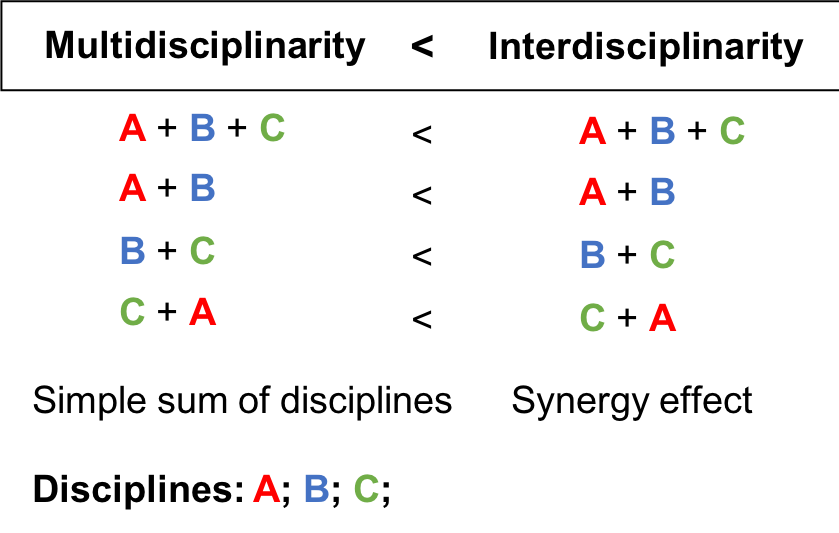
\includegraphics[width=0.6\linewidth]{figures-ext/multidisc} 

}

\caption[Symbolic illustration of a sum (multidisciplinarity) versus synergy (interdisciplinarity)]{\textbf{Symbolic illustration of a sum
(multidisciplinarity) versus synergy (interdisciplinarity)}, in an
interdisciplinary project sum of thee disciplines A, B, C should have
more value than a simple sum of disciplines: an interdisciplinary
project should have an added value compared to a multidisciplinary one.}\label{fig:multidisc}
\end{figure}







Why are not all of the labs interdisciplinary?

\begin{quote}
\emph{Scientists tend to resist interdisciplinary inquiries into their
own territory. In many instances, such parochialism is founded on the
fear that intrusion from other disciplines would compete unfairly for
limited financial resources and thus diminish their own opportunity for
research} ---
\href{http://www.azquotes.com/author/28130-Hannes_Alfven}{Hannes Alfvén}
\end{quote}

Crossing frontiers is not an easy task, and it was quite difficult in
the beginnings of modern interdisciplinarity. Some examples of early
interdisciplinary efforts of the 20th century are nicely described by
Ledford et al. \citep{Ledford2015} in \emph{Nature} special issue on
\href{https://www.nature.com/news/interdisciplinarity-1.18295}{Interdisciplinarity}.
It illustrates Theodore Brown in 1980s while trying to organize a new
interdisciplinary research project and reorganize university space to
engage an exchange between students of different faculties, and he
encounters a lot of reluctance.

\begin{quote}
\emph{And then there was the stigma. ``Interdisciplinary research is for
people who aren't good enough to make it in their own field,'' an
illustrious physicist chided} \citep{Ledford2015}.
\end{quote}

The story seems to end up with a happy ending of 40-million US dollars
grant and foundation of Beckman Institute for Advanced Science and
Technology. However, recruiting an open-minded director for leading this
unconventional organization was a struggle. Shortly, the structure
became a model for others and met a great scientific and technological
success.

Even though, since then the idea of interdisciplinary research spread
around the world. Yet, not all problems were overcome.

\begin{quote}
\emph{``There's a huge push to call your work interdisciplinary,'' says
David Wood, a bioengineer at the University of Minnesota in Minneapolis.
``But there's still resistance to doing actual interdisciplinary
science''.}
\end{quote}

First, the institutions, universities where research is performed should
equip scientist with a passport to other disciplines, facilitate
exchange, funding the interdisciplinary research, be accepting fusion of
disciplines as new ones. Then, proper communication between disciplines
is necessary. Finally, developing interdisciplinary research is
extremely challenging as it often requires extra effort from an
apprentice.

\emph{Are all the disciplines independent units nowadays?}

Can we do molecular biology without technical, mathematical and
computational support? Can we study cognitive science without knowledge
of biology, physics, and psychology? Can we advance medicine without
basic research in biology, physiology, electronics?

Bioinformatics and/or computational biology is an compelling case.
Working in this field is being between biology, medicine, computer
science, mathematics and statistics, the role of a computational
biologist is sometimes reduced to a service. A biological lab may need a
computational biologist to perform an analysis, restructure the data,
that is needed for the biological discovery. Often, there is not enough
space for research in computational biology itself, where the discovery
does not depend on the original data but tools and approaches to
complex, data-intensive biological problems. It may also happen the
other way round when a computational biologist asks a bench researcher
to perform an experiment to prove his theoretical model. In both cases,
the long-term interdisciplinary partnership would probably fail. Wet and
dry researchers should collaborate as equal with important research
advances on both sides to assure a long-term equilibrium.

\emph{How did interdisciplinarity change over the years? Are all
disciplines affected equally?}

From the chart (Fig. \ref{fig:interdisciplinary}), we can notice that
Social Studies of Medicine seems to be the most interdisciplinary field.
In general Biology, Health and Biomedical Sciences seem to be more open
into a flow of knowledge from other fields than humanities. On the
extreme opposite of health, Clinical Medicine appears to be a very
conservative field.

\begin{figure}

{\centering 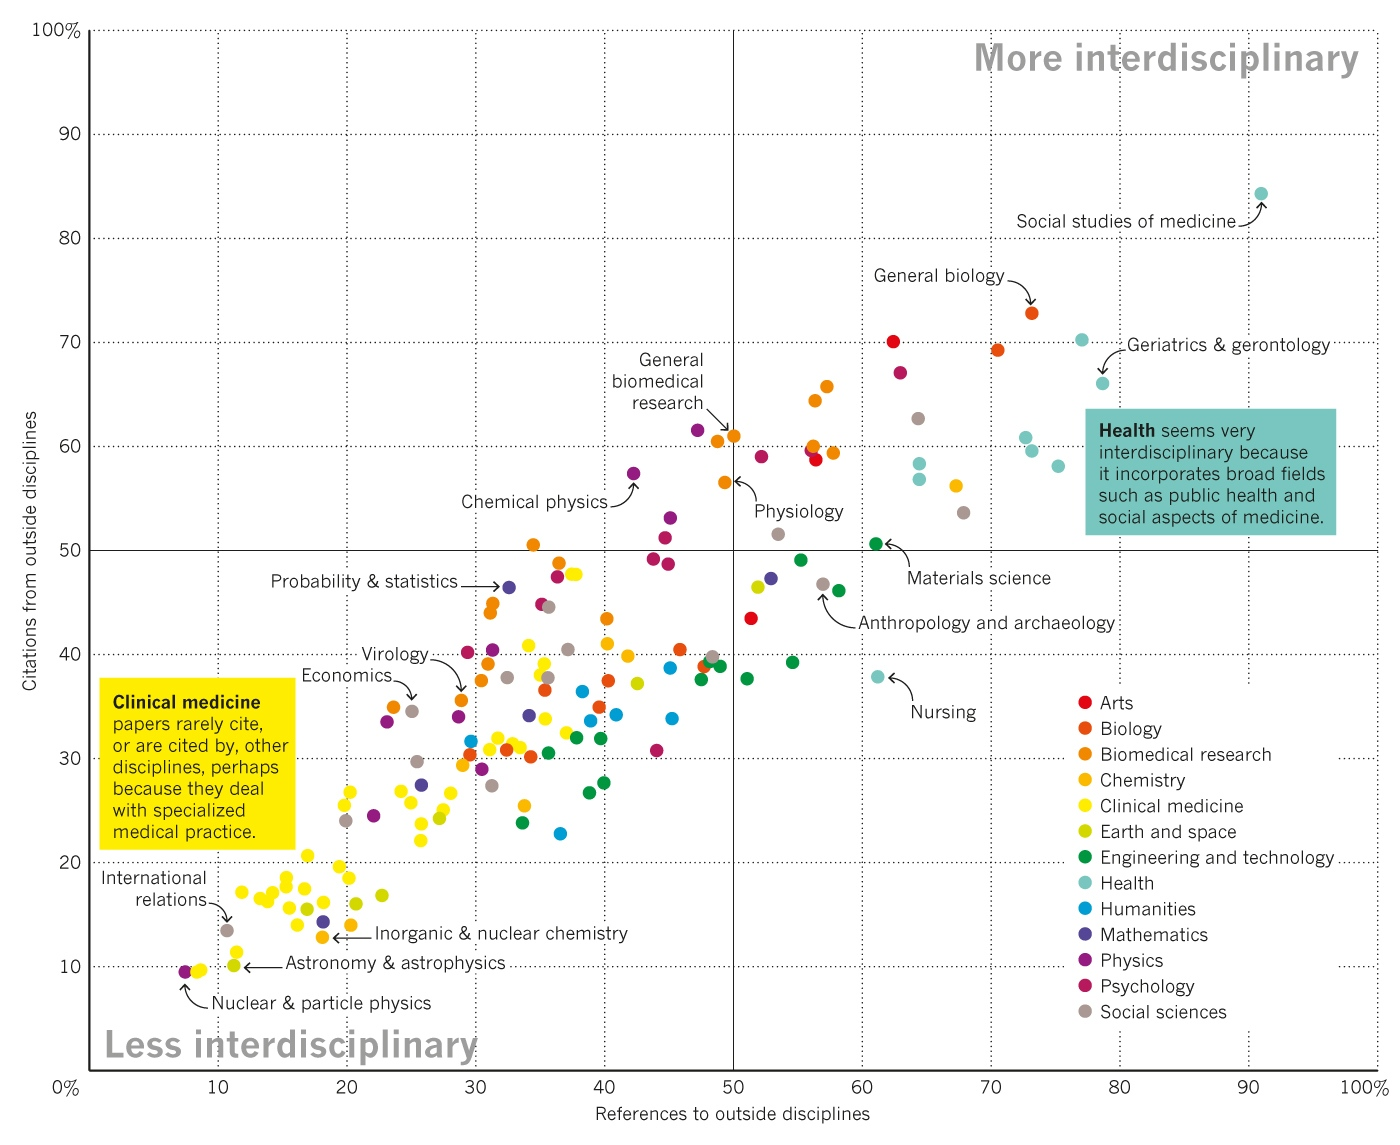
\includegraphics[width=0.9\linewidth]{figures-ext/interdisciplinary} 

}

\caption[Interdisciplinarity of different fields.]{\textbf{Interdisciplinarity of different
fields.} ``From 1950-2014, a field's position is determined by how much
its papers cite outside disciplines (x-axis), and by how much outside
disciplines subsequently cite its papers (y-axis). (Some years, certain
fields have too few references to be plotted.)''. Reprinted by
permission from Springer Nature \citep{VanNoorden2015} © 2015 Nature
America, Inc.~All rights reserved.}\label{fig:interdisciplinary}
\end{figure}









\hypertarget{strengths-weaknesses-opportunities-threats-swot-of-an-interdisciplinary-ph.d.---personal-perspective}{%
\section*{Strengths, Weaknesses Opportunities, Threats (SWOT) of an
interdisciplinary Ph.D. - personal
perspective}\label{strengths-weaknesses-opportunities-threats-swot-of-an-interdisciplinary-ph.d.---personal-perspective}}
\addcontentsline{toc}{section}{Strengths, Weaknesses Opportunities,
Threats (SWOT) of an interdisciplinary Ph.D. - personal perspective}

\begin{quote}
\emph{I'm not good enough to do well something I dislike. In fact, I
find it hard enough to do well something that I like} --- Jim Watson,
Succeeding In Science: Some Rules Of Thumb \citep{Csermely2007}
\end{quote}

Being formed first in a double major in biology and mathematics, then
participating in interdisciplinary research projects during my master
studies, I can witness that the learning curve of multiple disciplines
can be steep. It is also often associated with the frustration of not
going deep enough in all of the disciplines or the feeling of being
overwhelmed by the amount of knowledge.

Coming with the expertise in biology and mathematics, I got fascinated
by complex biological systems. One way of study high-dimensional data is
to reduce them into smaller interpretable units. This is what I tempted
to achieve in this thesis in order to enrich our knowledge about tumor
microenvironment and possibly contribute to orienting future research on
immunotherapies.

However, being an interdisciplinary researcher was not always a
privilege. \emph{To which category do I belong?} \emph{To whom should I
present my work?} I often asked myself these questions. I also often
encountered lack of understanding where my methodological results were
not bringing enough of \emph{biological insights}. Or the constraints of
my biological application seemed very obscured and complicated for
mathematicians, and my work often lacked \emph{important methodological
advances}.

\emph{Does it mean that my work is not accurate, useless?} Probably, for
many, it is not enough. However, I still hope that our findings will be
interesting to some. I enjoy working with data and statistics that serve
an actual purpose. The Tab. \ref{tab:SWOT} summarizes Strengths,
Weaknesses, Opportunities, and Threats (SWOT analysis) of an
interdisciplinary project, in the way I perceive it.

\rowcolors{2}{gray!6}{white}\begin{table}

\caption[SWOT analysis of Interdisciplinary research]{\label{tab:SWOT}\textbf{SWOT analysis of Interdisciplinary research}.
In SWOT analysis, Strengths, Weaknesses, Opportunities, and Threats are
enumerated. Strengths and Weaknesses are internal, and Opportunities and
Threats are external factors.}
\centering
\begin{tabular}[t]{|>{\centering\arraybackslash}p{9em}|>{\centering\arraybackslash}p{9em}|>{\centering\arraybackslash}p{9em}|>{\centering\arraybackslash}p{9em}|}
\hiderowcolors
\toprule
\rowcolor{Gray}  \textcolor{white}{\textbf{Strengths (internal, positive)}} & \textcolor{white}{\textbf{Weaknesses (internal, negative)}} & \textcolor{white}{\textbf{Opportunities (external, positive)}} & \textcolor{white}{\textbf{Threats (external, negative)}}\\
\midrule
\showrowcolors
Having a holistic view of the problem & Not seeing details of the problem & Mulitple possibilities to convey research & Spending too much time filling knowledge gap\\
Being supervised by multiple experts & Following multiple, sometimes contradictory,  advice on the same problem & Take advantage of synergistic effect of fields & Inhibiting effect of oppinions from different fields\\
Joining expertises of different fields & Not covering in details all the disciplines & Doing a new discovery & Obtaining too generic results\\
Using new/non standard approach & Experiencing steep learning curve & Raising interest in different expert domains & Not mastering the specific vocabulary of different fields\\
Having better understanding of complex processes & Being in constant need of help of domain experts & Making progress & Not being understood\\
\addlinespace
Higher creativity &  & Creating a new field & Being hard to classify/ fall into a category\\
Having great flexibility &  & Sovling many problems impossible to solve with traditional approach & Being considered as superficial\\
Feeling a thrill of adventure &  &  & \\
Being open &  &  & \\
\bottomrule
\end{tabular}
\end{table}\rowcolors{2}{white}{white}






Besides conducting research that crosses the boundaries of one
discipline, I also could meet and work with inspiring people coping like
me with filling the gap in understanding of interdisciplinary work,
multiple supervisors and report to many institutions. I gained (even if
only superficial) understanding of many topics in mathematics,
statistics, data science, immunology, cancer but also oral and written
presentation skills, time and work management

Is my thesis genuinely interdisciplinary? Does biology profits from
mathematics and mathematics from biology? I will let you judge it.

What impact had biology on the statistical/mathematical modeling? The
practical problems, systems that go beyond theoretical formulations
challenge the theoretical tools. In my work, I did my best to fuse
theory and practice that should serve a biological application. I can
image the project more complete if the results of my work would inspire
changes in biological experiments, uncover new paths to follow for
experimental biologists or translational researchers.

\hypertarget{the-origins-of-the-ph.d.topic}{%
\section*{The origins of the
Ph.D.~topic}\label{the-origins-of-the-ph.d.topic}}
\addcontentsline{toc}{section}{The origins of the Ph.D.~topic}

\begin{quote}
\emph{The universe will lead me where I need to go. I am like a leaf in
the stream of creation} --- Dirk Gently, Holistic detective
\end{quote}

When finishing my master, I was looking for an interdisciplinary topic
where I could deepen my quantitative skills and apply to a real-life
healthcare problem. I came across a project proposed by Andrei Zinovyev
in close collaboration with Vassili Soumelis. I was quite anxious that
my knowledge of cancer immunology would not be sufficient to lead the
project to a success. I recognize that the immune systems are very
complex and dynamic system and many years of expertise are needed to
grasp an understanding of it really. I had a great chance to work hand
in hand with domain experts that would suggest me the direction I should
take in my research.

The project started by causal exploration of different blind source
separation or dimension reduction techniques and their ability to
dissect bulk transcriptomic data into cell type-related units. We also
faced a vital problem of lack of gold standard validation data that
would define efficiency and accuracy of different methods.

I have spent fruitless efforts working on a bulk transcriptomic data
simulation framework, important statistical issues come our way and
probably another few years of a different Ph.D.~would be necessary to
solve them. In the meantime, many tools dissecting tumor bulk
transcriptome were published. Serving a similar purpose, they used
different means and assumptions, which left a space for my project to
continue. In my third year, I am finally publishing a tool that performs
the analysis I developed together with the Sysbio team members, and I
can apply it to a corpus of publicly available data to learn about the
actual question: the immune system infiltrating cancers and the
context-dependent signatures (see \protect\hyperlink{deconica}{Chapters
4 \& 5}).

In a parallel project, I worked on an exploration of a brand new data
type: single cell transcriptomic (RNAseq) in the context of tumor
microenvironment (see \protect\hyperlink{map}{Chapter 6}).

We have also participated in the Dream Idea Challenge, a project that
aimed to put closer experimental and theoretical researchers
(\protect\hyperlink{annex1}{Annexe 1}, \citep{Azencott2017}) .

I have collaborated in numerous projects within and outside my team.
Some of the projects resulted in publications, such as my work on
analyzing pDC subsets of breast cancer
\protect\hyperlink{annexe2}{Annexe2}. Some others are in still
preparation.

I have attended nine national, and international conferences, where I
presented posters, gave talks and I got awarded with distinctions for my
work.

Alongside with pursuing the compelling scientific research, I completed
a wide variety of courses and I was teaching IT, Statistics and
Mathematics at pharmacology faculty. Thanks to this extensive
(\textgreater{}300 hours) training over three years, I am equipped with
soft skills that not only helped me to shape my thesis project on the go
but also, I hope, will help me to succeed in my future career path.

\hypertarget{organisation-of-the-dissertation}{%
\chapter*{Organisation of the
dissertation}\label{organisation-of-the-dissertation}}
\addcontentsline{toc}{chapter}{Organisation of the dissertation}

\chaptermark{Organisation of the dissertation}

As it is a fruit of an interdisciplinary work, I decided to introduce
the topic from two perspectives: describe the biological and biomedical
dimension of the topic (see \protect\hyperlink{intro}{Chapter 1}), as
well as, the mathematical dimension of the problem of separation of
sources in complex mixtures (see \protect\hyperlink{methods}{Chapter
2}). I hope, it will make the subject of my thesis easy to understand
also for non-biologists or non-mathematicians. In the results part, I
introduce a study of ICA applied to transcriptomes
(\protect\hyperlink{mstd}{Chapter 3}). I also apply ICA-based
deconvolution to Breast cancer transcriptomes to prove its
reproducibility \protect\hyperlink{LVA}{Chapter 4}. I compare the
reproducibility of blind source separation methods NMF and ICA (see
\protect\hyperlink{nmfica}{Chapter 5}). Then I introduce the DeconICA R
package (see \protect\hyperlink{deconica}{Chapter 6} ) and finally
present results of an application of DeconICA and other tools to 118
transcriptomic datasets (see \protect\hyperlink{results}{Chapter 7}).
The second part of the results is dedicated to my work on cell type
heterogeneity (see \protect\hyperlink{map}{Chapter 8}). The manuscript
finishes with \protect\hyperlink{discussiongenerale}{Chapter 9} and
\protect\hyperlink{conclusions}{Chapter 10} that contain discussion,
conclusions, and perspectives. In annexes, you can find publications to
which I contributed during my doctorate that are not strictly linked
with the topic of this thesis. In the end, I included a glossary of
useful terms.

\textbf{INTRODUCTION}

\begin{itemize}
\item
  \protect\hyperlink{intro}{Chapter 1}: introduction to cancer biology
  and immunity, challenges in cancer immunotherapies and cancer immune
  phenotyping as well as data sources most commonly used to face the
  topic.
\item
  \protect\hyperlink{methods}{Chapter 2}: introduction to a problem of
  mixed sources in biological samples, an overview of blind source
  separation methods and supervised deconvolution methods, with focus on
  those applied to bulk transcriptome to uncover and quantify immune
  compartments
\end{itemize}

\textbf{RESULTS}

\begin{itemize}
\tightlist
\item
  \protect\hyperlink{mstd}{Chapter 3}: Most Reproducible Transcriptome
  Dimension (MSTD)
\item
  \href{}{Chapter 4}: application of ICA-based deconvolution to six
  breast transcriptomes
\item
  \protect\hyperlink{sens}{Chapter 5}: comparison of reproducibility of
  NMF and ICA methods
\item
  \href{}{Chapter 6}: DeconICA R package
\item
  \href{}{Chapter 7}: application of DeconICA R package and other tools
  to analyze \textgreater{}100 transcriptome datasets of bulk cancer
  transcriptomes
\item
  \protect\hyperlink{map}{Chapter 8}: study of immune cell types
  heterogeneity in tumor microenvironment using the innate immune map
  and scRNA-seq data
\end{itemize}

\textbf{DISCUSSION}

\begin{itemize}
\tightlist
\item
  \protect\hyperlink{discussiongenerale}{Chapter 9}: Discussion
\item
  \protect\hyperlink{conclusions}{Chapter 10}: Conclusions and
  perspectives
\end{itemize}

\textbf{ANNEXES}

\begin{itemize}
\tightlist
\item
  Other publications:

  \begin{itemize}
  \tightlist
  \item
    Adjustment of dendritic cells to the breast-cancer microenvironment
    is subset specific
  \item
    The inconvenience of data of convenience: computational research
    beyond post-mortem analyses
  \end{itemize}
\item
  DeconICA R package documentation:

  \begin{itemize}
  \tightlist
  \item
    Vignette 1: Introduction to deconICA
  \item
    Vignette 2: Running fastICA with icasso stabilization
  \item
    Manual
  \end{itemize}
\item
  Scientific CV (including a list of attended conferences and
  publications)
\end{itemize}

\textbf{GLOSSARY}

\hypertarget{part-introduction}{%
\part{Introduction}\label{part-introduction}}

\hypertarget{intro}{%
\chapter{Immuno-biology of cancer}\label{intro}}

This chapter will first introduce a short history of cancer with a focus
on discoveries linking cancer and its environment. It will also describe
the participation of TME in cancer development, progression and response
to treatment. Most important types of data used to study cancer
microenvironment will be discussed. I also introduce a link between
tumor immune-biology and cancer phenotyping for development of
immunotherapies.

\hypertarget{cancer-disease}{%
\section{Cancer disease}\label{cancer-disease}}

According to
\href{http://globocan.iarc.fr/Pages/fact_sheets_cancer.aspx}{GLOBOCAN
study} \citep{GLOBOCAN}, 14.1 million cancer cases were estimated to
happen around the world in 2012. It touched 7.4 million men and 6.7
million women. It is estimated that the cancer cases will increase
almost two-fold to 24 million by 2035.

In France only, in 2012 there were 349426 cases of cancer, of which
leading is Prostate cancer (16,3\%) followed by Breast (14\%) and Lung
(11,5\%).

For a long time studying tumor was focused on tumor cells, their
reprogramming, mutations. Cancer was seen as a disease of uncontrolled
cells by the mainstream research. At the same time, the idea of the
importance of the impact of other cells and structures on cancer cells
was present but often not believed. A recent success of immunotherapies
moved research focus to tumor cells in their context: tumor
microenvironment. We will describe here what is the composition and role
of the TME in tumor progression, diagnosis and response to treatment.

\hypertarget{hist}{%
\subsection{Historical understanding of cancer}\label{hist}}

Cancer was historically described by a physician Hippocrates (460--370
B.C) \citep{Sudhakar2009}. Even though there exist even earlier evidence
of the disease. Hippocrates stated that the body contained 4 humors
(body fluids): blood, phlegm, yellow bile and black bile. Any imbalance
of these fluids will result in disease. Particularly the excess of black
bile in an organ was meant to provoke cancer. For years, it was not
known what factors cause cancer and it was easily confounded with other
diseases. In the middle ages in the Renaissance Period, it was believed
cancer is a punishment for the sins they committed against their god,
that they deserved it to some extent.

Until the 18th century, it was believed that cancer is contagious and is
spread by parasites.

In the 19th century, tumor cells started to be analyzed by pathologists.
They were strike with their ability to proliferate uncontrollably,
ability to spread and destroy the original tissue \citep{NPR2010}.
Around the same time, leukocytes from the blood were first described by
Gabriel Andra and William Addison. Just a few years later, in 1845
Bennett and Virchow described blood cells in leukemia (Fig.
\ref{fig:Virchow-cell}). Virchow is also a father of Chronic irritation
theory (nowadays called chronic inflammation) that says that cancer is
caused by local ``irritation'' and, incorrectly, that cancer cells
spread like liquid resulting in metastasis.

\begin{figure}

{\centering 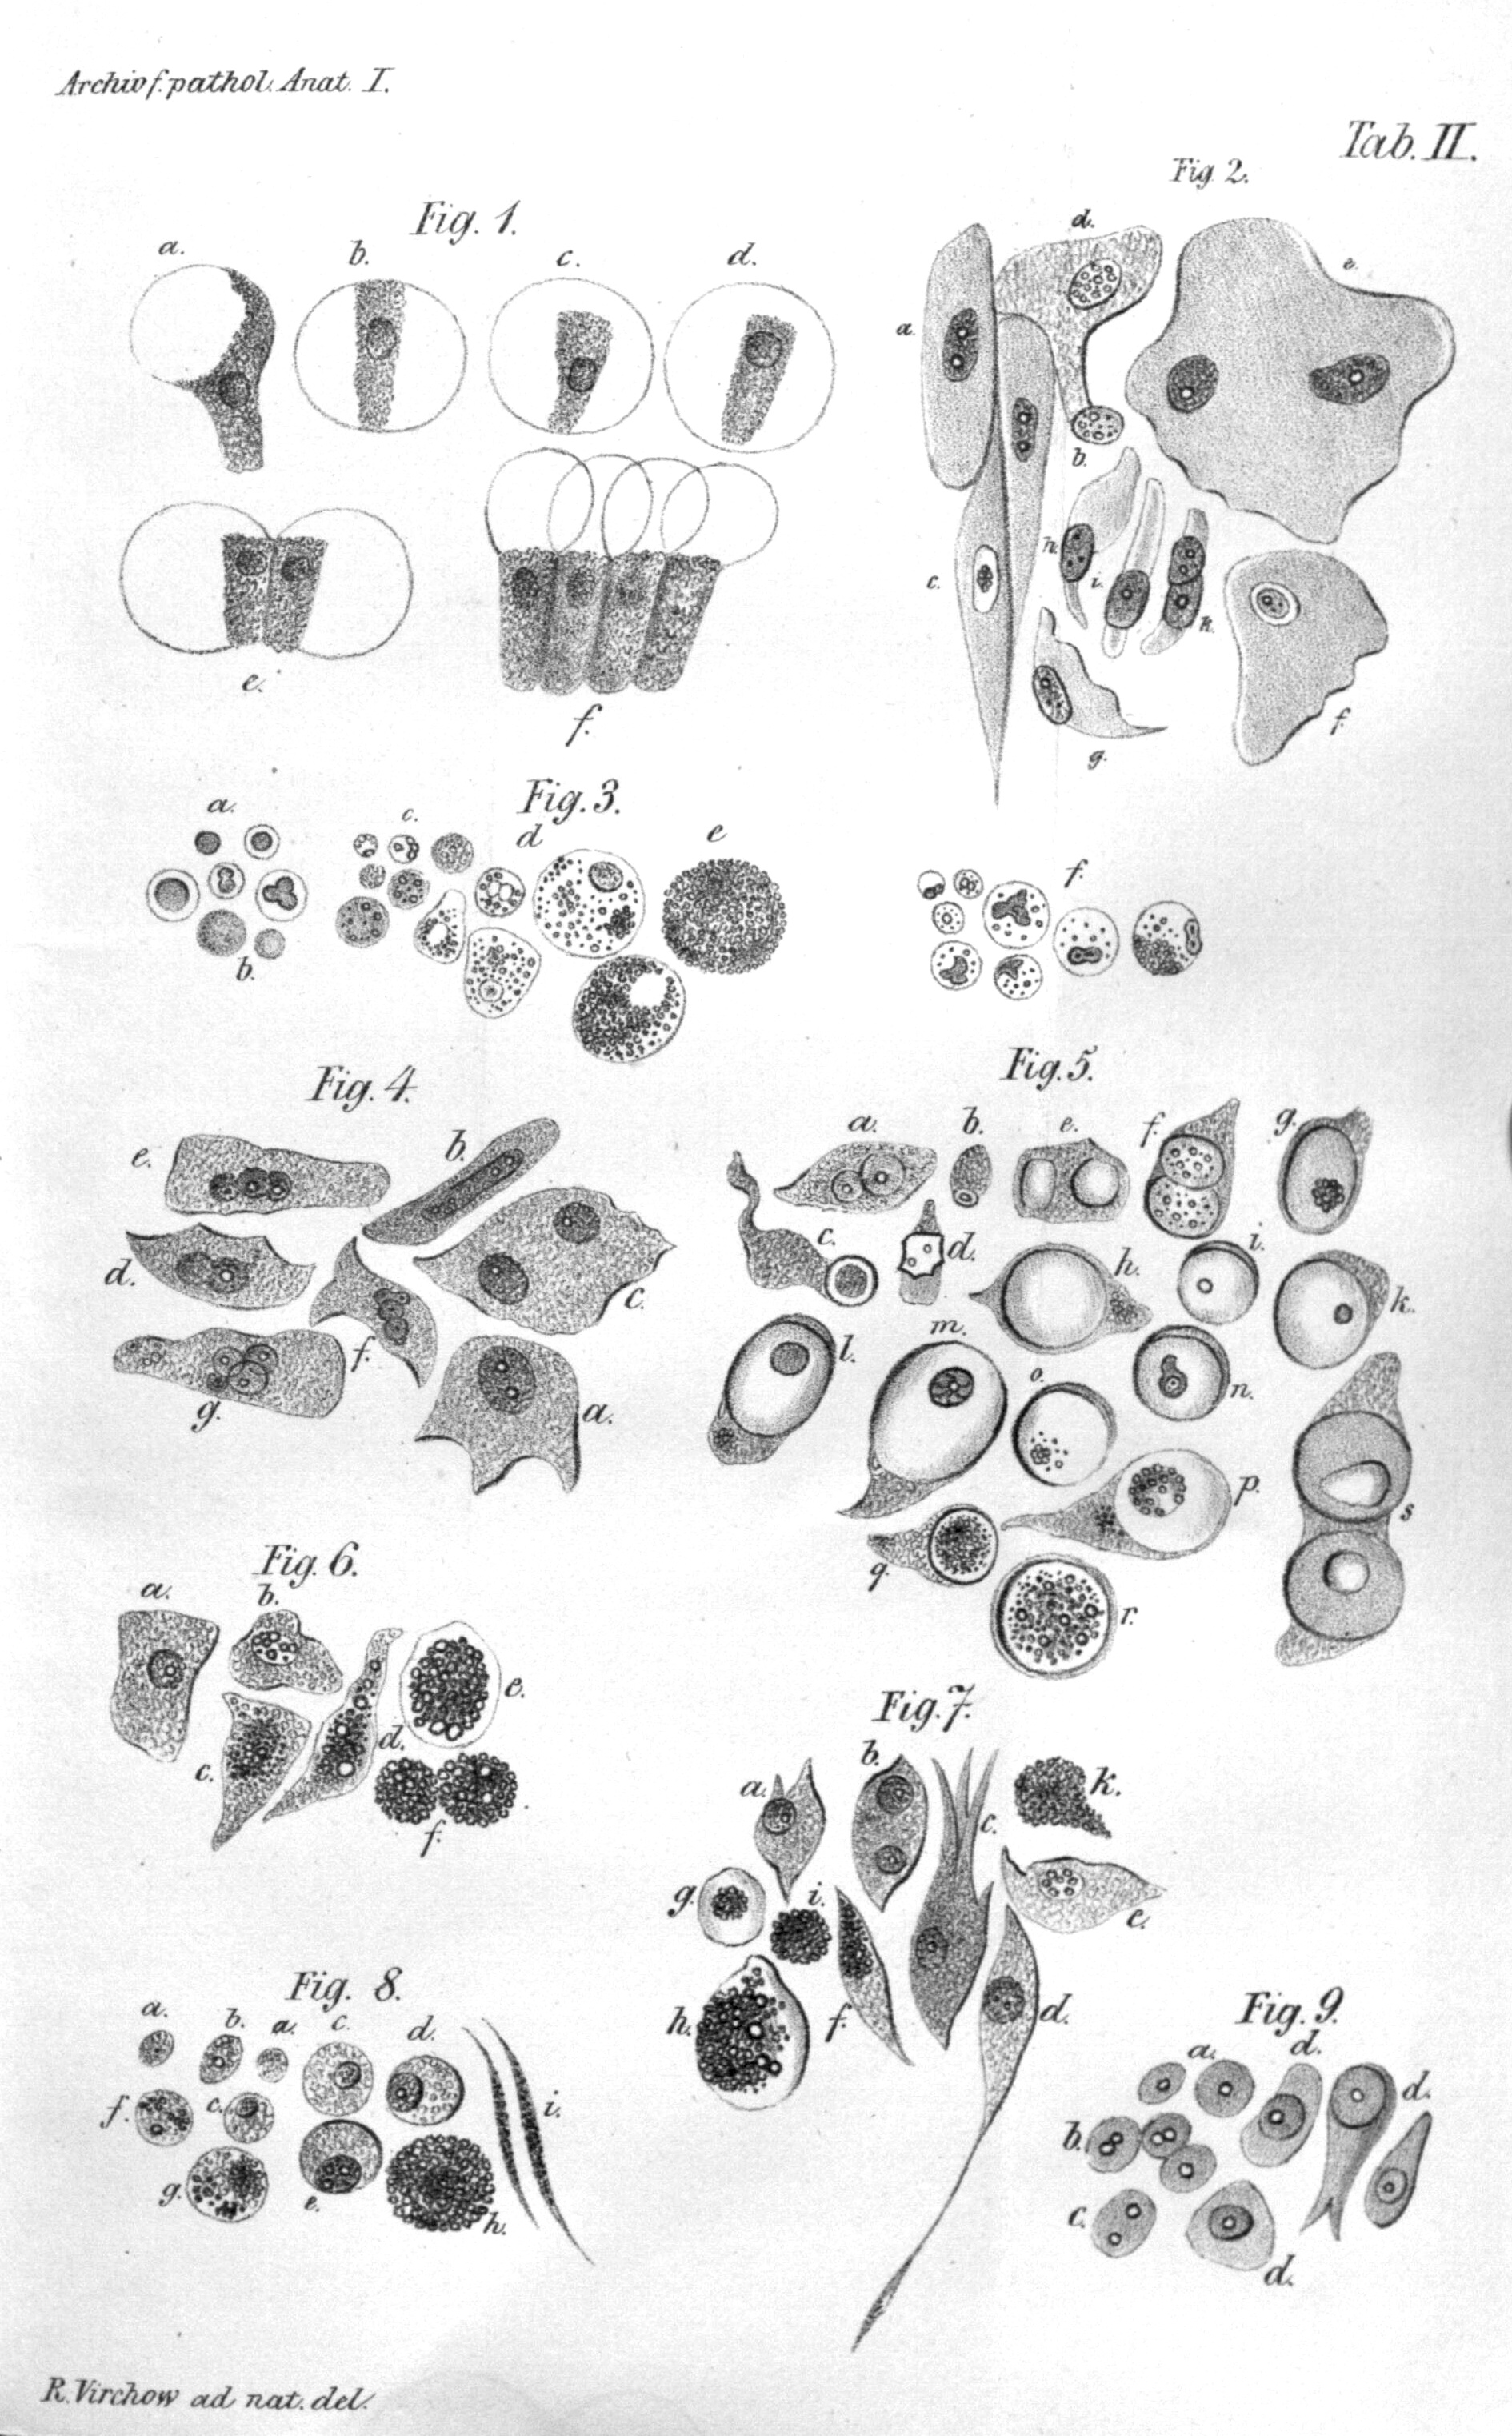
\includegraphics[width=1\linewidth]{figures-ext/01-Virchow-cell} 

}

\caption[Illustration of Virchow's cell theory]{\textbf{Illustration of Virchow's cell
theory}. Virchow depicted different cells transformation due to
irritation. \citep{VirchowRudolf1847}}\label{fig:Virchow-cell}
\end{figure}





In 1889, Stephen Paget introduced \emph{soil and seed} hypothesis of
metastases \citep{Paget1889}. He formulates it as follows

\begin{quote}
\emph{When a plant goes to seed, its seeds are carried in all
directions, but they can only live and grow if they fall on congenial
soil.}
\end{quote}

Which is parallel to cancer cells disseminated by body fluids, and they
can grow only tissues - ``soil'' that is predisposed to host the cancer
cell - ``the seed''. He focused on the importance of tissue
characteristics that favorize tumor development as opposed to most
researchers of his time that were focusing on the ``seed'' itself.

In the 20th century, molecular causes started to be investigated. It was
discovered that cancer could be caused by environmental factors,
i.e.~chemicals (carcinogens), radiation, viruses and also inherited from
ancestors. Those factors would damage but contrary to a healthy
condition they would not die.

Also in 1909, Paul Ehrlich, called one of fathers of immunology and
Nobel Prize laureate, indicated a link between immune system and tumor
suppression \citep{Ehrlich1909}. One of the remarkable first
immunotherapy attempts can be attributed to William Coley, that
practiced injecting streptococcus bacteria directly into patients after
cancer surgery in 1891, later called ``Colley vaccine''. However, the
impact of this procedure on patients recovery was judged by scientific
community as ``unclear''.

In 1968, Melvin Greenblatt and Philippe Shubik showed that tumor
transplants secrete a substance stimulating the growth of blood vessels
\citep{Greenblatt1968}, later identified as ``tumor angiogenic factor
(TAF)'' by Judah Folkman in 1971 \citep{Folkman1971}. Folkman also
suggested that TAF can be a target of a therapy itself. This was a
revolutionary idea, at the time, as it did not target the tumor cells
directly acted on their environment.

During the 1970s, oncogenes and tumor suppressor genes were discovered.
Oncogenes are genes that allow a cell to become a cancer cell, while the
tumor suppressor genes would repair DNA or execute cell death of a
damaged cell. A new dimension to cancer studies was added in the 1980s,
epigenetic changes were proven to occur to both oncogenes and tumor
suppressors \citep{Feinberg1983, Greger1989}, which are presently known
as epigenetic markers used for diagnostics and therapeutic targets for
cancer.

In 1982, Aline van Pel and Thierry Boon \citep{VanPel1982} discovered
that a specific immunity to spontaneous tumor cells could be induced by
vaccinating mice with mutagenized tumor cells. This raised an
inspiration for many years of immune therapy development.

In Napoleone Ferrara and colleagues identified the gene encoding
vascular endothelial growth factor (VEGF) that was shown to stimulate
the growth of endothelial cells proliferation \emph{in vitro} and
angiogenesis (blood vessels formation) \emph{in vivo} \citep{Leung1989}.

In 1999 for the first time, gene-expression was used to study cancer
(leukemia) by Todd Golub, Donna Slonim and colleagues \citep{Golub1999}.

Since the end of the 20th century, cancer screens are developed along
with multiple strategies to fight the tumor. Most classical ones are
based on the idea of removing tumor cells (surgery), killing tumor cells
with DNA-blocking drugs (chemotherapy), radiation, inhibit cancer growth
(hormonal therapy, adjuvant therapy and immunotherapy). As none of those
methods is fully efficient, often a combination of treatments is
proposed. Nowadays, science is aiming in the direction of targeted
therapies and personalized treatment.

The recent success of immunotherapies (discussed in
\protect\hyperlink{immunotherapies}{Immunotherapies section} attracted
the attention the scientific community again to the context in which
tumor cells are found. This context called Tumor Microenvironment, as
well as the communication that happens within it between different
agents nowadays studied differently with available knowledge of
molecular biology, have become a popular scientific topic of the 21st
century (Fig. \ref{fig:pubmedTME}).

\begin{figure}

{\centering 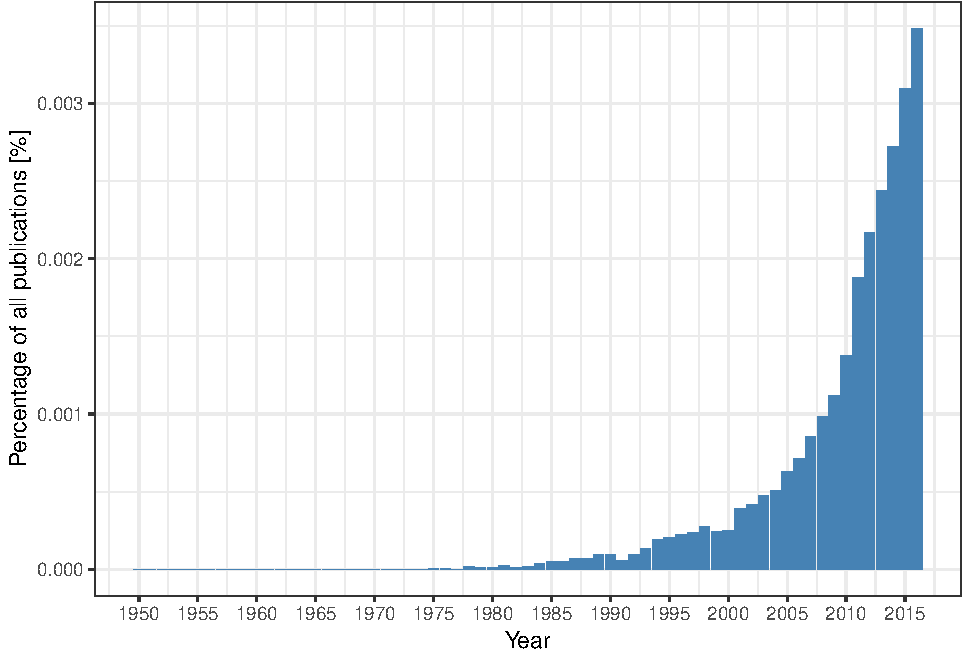
\includegraphics[width=0.7\linewidth]{UCzPhDThesis_files/figure-latex/pubmedTME-1} 

}

\caption[Percentage of publications containing the phrase "tumor immunotherapy" is growing]{\textbf{Percentage of publications containing
the phrase ``tumor immunotherapy'' is growing}, numbers retrieved on
17.01.2018 from \href{http://dan.corlan.net/medline-trend.html}{Medline
Trends} \citep{Corlan2004}}\label{fig:pubmedTME}
\end{figure}






\hypertarget{tumor-microenvironment-as-a-complex-system}{%
\subsection{Tumor Microenvironment as a complex
system}\label{tumor-microenvironment-as-a-complex-system}}

Tumor Microenvironment is a complex tissue that surrounds tumor cells.
It is composed of different compartments (in solid tumors):

\begin{itemize}
\tightlist
\item
  Stroma: blood and lymphatics vessels, epithelial cells, mesenchymal
  stem cells, fibroblasts, adipocytes supported by extracellular matrix
  (EM)
\item
  Immune cells: T cells, B cells, NK cells, Dendritic cells,
  Macrophages, Monocytes etc.
\end{itemize}

Their proportion and specific roles vary significantly with tumor type
and stage. Communication between the environmental cells and the tumor
is critical for tumor development and has an impact on patient's
response to treatment. This communication between different compartments
is bidirectional and all the players can influence each other. Depending
on the nature and prevailing direction of those interactions different
destiny is possible for each of the compartments, i.e.~immune cells can
be recruited to protect tumor cells or they can kill them directly. Many
of the signals can be contradictory, many can suppress each other. Then
is it possible to tilt this complex ecosystem into patients' favor? Can
we decipher the most important factors of this molecular knot and
manipulate it?

Next section describes different scenarios of interaction within TME in
order to illustrate the complexity of TME and possible targets for
cancer therapies.

\hypertarget{interactions-between-tme-and-tumor}{%
\subsubsection{Interactions between TME and
Tumor}\label{interactions-between-tme-and-tumor}}

Three scenarios can be considered to describe the relationship between
TME and tumor cells:

\begin{enumerate}
\def\labelenumi{\arabic{enumi}.}
\tightlist
\item
  TME stimulates tumor growth and/or progression and/or impact
  negatively the response to treatment
\item
  TME has no influence on tumor cells and disease development
\item
  TME has a tumor-suppressive role and impact positively the response to
  treatment
\end{enumerate}

As it is presented in \protect\hyperlink{hist}{Section 1.1.1} these
three hypotheses were gaining and losing popularity in the scientific
and medical community over the decades.

\hypertarget{tme-as-a-foe-inflammation}{%
\paragraph{TME as a foe: inflammation}\label{tme-as-a-foe-inflammation}}

In 1863 Rudolf Virchow observed a link between chronic inflammation and
tumorigenesis. According to Virchov theory, the genetic damage would be
the ``match that lights the fire'' of cancer, and the inflammation or
cytokines produced by immune cells should be the ``fuel that feeds the
flames'' \citep{Balkwill2001}. Therefore lymphocyte infiltration was
confirmed by subsequent studies as a hallmark o cancer. The question one
may ask is why our immune system is not enough to defend the organism
from tumor cells as it does efficiently in a range of bacterial and
viral infections? It is mainly because of the ability of tumor cells to
inhibit immune response through activation of negative regulatory
pathways (so-called immune checkpoints).

It is worth mentioning, that the immune system can be already disabled
and therefore cancer has more facility to develop. The immune system can
be less efficient for example because of drugs given to patients after
transplants of because of diseases like HIV/AIDS. These people have
higher probability to develop cancers caused by infectious agents
(viruses). These cancers are non-Hodgkin lymphoma (NHL) (caused by
\href{https://www.cancer.gov/Common/PopUps/popDefinition.aspx?id=CDR0000045684\&version=Patient\&language=English}{Epstein-Barr
virus} (EBV) infection), lung (no identified specific infectious agent),
kidney (no identified specific infectious agent) and liver (caused by
chronic infection with the
\href{https://www.cancer.gov/Common/PopUps/popDefinition.aspx?id=CDR0000046146\&version=Patient\&language=English}{hepatitis
B} (HBV) and
\href{https://www.cancer.gov/Common/PopUps/popDefinition.aspx?id=CDR0000044139\&version=Patient\&language=English}{hepatitis
C} (HCV) viruses) cancers. Human papillomavirus (HPV), can cause
cervical, anal, oropharyngeal, and other cancers.

In the case of non-infectious cancers in patients with no history of
immunosuppressive drugs intake or diseases, the question how tumor
manages to break natural defence remains even more interesting. Many
examples can be cited on how TME facilitates tumor development (Fig.
\ref{fig:met-dis}). For instance, in the early stages of tumorigenesis,
some macrophage phenotypes support tumor growth and mobility through
TGF-beta signaling. Also, it was shown that NK cells and myeloid-derived
suppressor cells (MDSCs) have an ability to suppress immune defence
i.e.~immunosurveillance by dendritic cells (DCs), T cell activation and
macrophage polarisation and they promote tumor vascularization as well.
\citep{Talmadge2013, Gabrilovich2012} They create so-called niches that
facilitate tumor colonization. T-regs and myeloid-derived suppressor
cells can negatively impact natural immune defense and by these means
allow growth and invasion of tumor cells \citep{Taube2017a}. Another
cell type, a part of EM, fibroblast, or more precisely Cancer-Associated
Fibroblasts (CAFs) have proven pro-tumor functions in breast cancer
where they enhance metastasis \citep{Dumont2013}. The blood and
lymphatic vessels maintain tumor growth providing necessary nutritive
compound to malignant cells.

\begin{figure}

{\centering \includegraphics[width=1\linewidth]{figures-ext/massive-dissemination} 

}

\caption[The microenvironment supports metastatic dissemination and colonization at secondary sites.]{\textbf{The microenvironment supports metastatic
dissemination and colonization at secondary sites.} Different tumor
sites can communicate through exosomes realized by tumor cells and also
immune and stromal cells such as NK cells, CAFs and DCs. Reprinted by
permission from Springer Nature \citep{Quail2013} © 2013 Nature America,
Inc.~All rights reserved.}\label{fig:met-dis}
\end{figure}








According to \citep{Hanahan2012} immune and stroma cells participate in
almost all of Cancer Hallmarks \citep{Hanahan2000, Hanahan2012}. Most of
the hallmarks of cancer are enabled and sustained to varying degrees
through contributions from repertoires of stromal cell types and
distinctive subcell types.

\hypertarget{tme-seen-as-neutral}{%
\paragraph{TME seen as neutral}\label{tme-seen-as-neutral}}

In front of lack of definitive proof that TME can positively or
negatively impact on tumor development, many scientists, in a long time,
ignored the importance of this factor. Until the early-mid eighties, the
TME research was mostly limited to angiogenesis and immune environment
and most areas that are now driving the field were not represented.

From the early 70s until the end of the 90s. the most accepted statement
was that genetic alterations in oncogenes and tumor suppressor genes are
both necessary and sufficient to initiate tumorigenesis and drive tumor
progression. Therefore TME was not seen as an important element of the
puzzle.

The cancer geneticists, at the time, had a lot of influence on
scientific community diminishing the work made on TME which were
considered as ``uninteresting'' and definitely not ``mainstream''.

After the 90s, with the discovery of signaling molecules involved in the
communication of TME like VEGF general opinion started to change.
Furthermore, discoveries made by developmental biology field supported
the hypothesis that microenvironment plays an important role in
development which was later shown for tumorigenesis. Additionally, the
success of immune vaccines starting with the tuberculosis vaccine
Bacille Calmette-Guérin (BCG) in 1976 and finishing, at the moment with
checkpoint inhibitors did not leave the scientific community
indifferent.

\hypertarget{tme-as-a-friend-immunosurveillance}{%
\paragraph{TME as a friend:
immunosurveillance}\label{tme-as-a-friend-immunosurveillance}}

As mentioned in \protect\hyperlink{hist}{Section 1.1.1} Paget proposed a
hypothesis of ``seed and soil'' where the TME in a certain tissue (the
soil) can either stimulate or suppress the metastasis (the seed).
William Coley tested a possibility to trigger tumor-suppressive effect
via stimulation of the immune system with bacteria. In the 1960s, the
immune surveillance theory hypothesized ``the ability to identify and
destroy nascent tumors as a central asset of the immune system''
\citep{Sebeok1976, Burnet1970}. Thus, the hypothesis that TME can have a
positive role in tumor prognosis is not new.

In modern immuno-oncology, the term \emph{immune-editing} was introduced
by \citet{Dunn2002} in 2002, to describe~the relationship between the
tumor cells and the immune system. The immunosurveillance through
immune-editing can be summarized in three processes: elimination,
equilibrium, and escape \citep{Dunn2002}.

The elimination is the direct killing of cancer cells or growth
inhibition by the immune system. The adoptive T cells and NK are
actively involved in tumor killing and stimulate other immune cells. The
CD8 + cytotoxic lymphocytes (CTLs) directly recognize tumor cells.
Employing perforin- and granzyme-dependent mechanisms they can lyse
tumor cells. The CD4 + T cells release factors to induce proliferation
of B cells and to promote their differentiation to the antibody
(Ab)-secreting plasma cells, activate macrophages. Macrophages use
phagocytosis to eliminate cancer cells \citep{Vesely2011}.

The tumor-infiltrating lymphocytes (TILs) have been associated with an
overall good prognosis and better survival in different cancer studies.
Moreover, abundance of CD3 + and CD8 + T cells, NK cells, and
\(\gamma\delta\)T cells correlate with improved outcomes in epithelial
ovarian cancers \citep{Marquez-Medina2012}. Several studies report that
the presence of the abundant immune infiltrates is correlated with a
good prognosis or better survival
\citep{Kornstein1983, Baxevanis1994, Naito1998, Pages2005}. Spontaneous
regression of human tumors has been reported in cutaneous melanoma,
retinoblastoma, osteosarcoma, etc. \citep{Aris2012}.

The equilibrium is the phase when cancer and immune cells coexist and
their crosstalk is preventing metastasis.

T cells are the main actor in maintaining the equilibrium.
Progressively, the tumor cells become more immunogenic as they are not
edited by the immune system \citep{Bhatia2011}. The state of tumor cells
is then identified as ``dormant'' and active scientific reports
investigate the possible molecular pathways that maintain dormancy or
lead to escape \citep{Teng2008}.

The immune escape is the final process when tumor cells impair the
immune response.

\hypertarget{two-faced-nature-of-immune-cells-context-dependent-functional-plasticity}{%
\subsubsection{Two-faced nature of immune cells: context-dependent
functional
plasticity}\label{two-faced-nature-of-immune-cells-context-dependent-functional-plasticity}}

A modern vision of TME-tumor interactions assumes that tumor can be
directed to several molecular pathways. This direction is decided by
signals that are native of tumor cell and/or coming from the
microenvironment.

Recent studies unveil ambivalent nature of immune cells in TME. While
some as cytotoxic T cells, B cells and macrophages can manage to
eliminate tumor cells. Treg cells role is to regulate expansion and
activation of T and B cells. Depending on cancer type, they can be
either pro- or anti-tumor. For example, as it has been shown for T-regs,
that are usually associated with bad prognosis, they can be equally
associated with improved survival (i.e.~in colorectal cancer
\citep{Frey2010}). For innate immunity, there are widely accepted M1
(anti-tumor) and M2 (pro-tumor) extreme macrophages phenotypes in TME
\citep{Qian2010}. Most of the statements seem to be context dependent
and not valid universally across all cancer types. We already mentioned
Macrophages phenotypic plasticity as well as the different behavior of
EMC depending on tumor stage.

From a more general point of view, it has been observed that
immunodeficiency can correlate with high cancer incidence. Results of
analysis based on observations of 25,914 female immunosuppressed organ
transplant recipients, the tumor incidence was higher than predicted for
multiple cancers. However, the number of breast cancer cases decreased
which can be really disturbing if we need to decide on the role of
immune defense in tumor progression \citep{Stewart1995}. This indicates
that immune microenvironment can be cancer stimulating or inhibiting
depending on the type of cancer and/or other factors.

\hypertarget{immune-cell-subtypes-in-tme}{%
\subsubsection{Immune cell (sub)types in
TME}\label{immune-cell-subtypes-in-tme}}

We are taught that a cell is the basic structural, functional, and
biological unit of all known living organisms. A human body contains
around \(10^{14}\) which is three orders of magnitude more than the
number of stars in the Milky Way. This ensemble of cells is
traditionally classified into cell types based on their phenotypical
variety.

\begin{quote}
\emph{for their immense number, the variety of cells is much smaller:
only about 200 different cell types are represented in the collection of
about \(10^{14}\) cells that make up our bodies. These cells have
diverse capabilities and, superficially, have remarkably different
shapes\ldots{}.} \citet{Boal2002}
\end{quote}

In the description of TME, I have referred to cell types of immune cells
as well-established entities of the immune system. However, the
definition of cell types remains controversial and there is no consensus
among researchers on how exactly a cell type should be defined. The
notion of the cell-subtypes is even vaguer. The problem does not only
concerns immune cells, most of the cell types of our organism,
classified initially according to their morphology, seem to fulfill
multiple functions. One can also relate cell-type problem to species
problem where scientist also debates about where to draw the borders
between species. This problem is widely generalized as ``theory of
types'' \citep{Slater2013} in many disciplines as philosophy,
linguistics, mathematics.

In this chapter, I will limit the description to immune cell types.

An immune cell can be described nowadays along many axes:

\begin{itemize}
\tightlist
\item
  Phenotype /surface markers
\item
  Morphology (expressed proteins)
\item
  Ultrastructure (electron microscopy)
\item
  Molecular data (gene expression, genotype, epigenome)
\item
  Cell fate
\item
  Cell of origin
\item
  Function
\end{itemize}

Depending on how well a cell is different from all other cells along
with those axes, it will (or not) be defined as a distinct cell type.
Each of these axes contains a pièce of information that can agree with
other axis or not. These features can be independent or can overlap
depending on cell types in question. Historically, there were given
different importance based on the technologies and general tendencies.
Thus, there is no available general recipe applicable to discriminate
all cell types from each other. Moreover, usually, it is not possible to
measure all these axes simultaneously (because of the experimental,
money or other constraints). Therefore, depending on the scientific
question, different researches will give different weights to these axes
and a combination of 2-3 \emph{most important} features will be used to
discriminate cell types in a given study.

Besides, the discrimination of the cell types comes with more or less
subjective threshold on where the cells become \emph{significantly
different}. These thresholds can be established computationally or by an
expert. The usual practice is a mix of both methods.

Since the beginning of immunology, there was disagreement between
pre-defined cell types and cell functions.

\begin{quote}
\emph{Cette espèce de leucocytes a une grande ressemblance avec certains
éléments fixes du tissu conjonctif, ainsi qu'avec des cellules
endothéliales et des cellules de la pulpe splénique. On est donc souvent
embarrassé, surtout lorsqu'on trouve ces leucocytes mononucléaires en
dehors des vaisseaux, pour les distinguer des autres espèces de cellules
mentionnées.} --- Elie Metchnikoff, Leçons sur la pathologie comparée de
l'inflammation, 1891
\end{quote}

The definition of cell types and subtypes is widely discussed today with
the arrival of single cell technologies that allow a change of paradigm
in cell classifications. Up to now, the top-down approach was mostly
used. A pre-defined set of parameters describing a cell was fixed in
order to select cells and then other parameters were measured. Now, it
is possible to practice bottom-up approach where all (or some)
parameters are measured for a single cell and then, depending on its
distance from other cells, cell types are defined \citep{Satija2014}.

\begin{quote}
\emph{The concept of ``cell type'' is poorly defined and incredibly
useful}\\
--- Allon Klein, Harvard Medical School
\end{quote}

Researchers recognize that the concept of cell type is artificial and a
continuum of cell types is closer to the reality. According to Susanne
Rafelski,

\begin{quote}
\emph{A useful way to classify cells might thus be a multiscale and
multi-parameter cell-type space that includes vectors for key
intracellular organizational, dynamic, and functional features as well
as tissue location, gene expression etc.}
\end{quote}

Some, as Allon Klein, propose to introduce a concept of \emph{cell
states} which would better describe a cell depending on its context and
function. However, an emerging challenge would be to connect \emph{cell
states} with historical \emph{cell types.}
\citep{EdiorialCellSystems2017} .

Another aspect of cells, that I am not approaching in this thesis, is
time. Cells are shaped by their environment, intrinsic and extrinsic
events and can change states, functions etc. Can one cell belong to
different cell types depending on its trajectory? How to include the
dynamic aspect of the cells into the classification?

Thus, most scientists agree that used convention of cell types is not
ideal and it is more matter of convenience than biological reality. This
leaves a room to study cells and challenge existing classification.
Describing cell types or cell states in the tumor microenvironment is
extremely interesting as still little is know about the diversity of
cell infiltrated in solid tissues.

\hypertarget{summary}{%
\subsubsection{Summary}\label{summary}}

Cancer is a disease concerning milliards of people with a long history.
Scientific community recognizes the role of the environment where the
tumor cells find themselves as an important factor influencing tumor
development, prognosis and response to treatment. TME is a complex
environment that constantly interacts with tumor cells, where both tumor
and TME influence and shape each other.

Over the years, many interactions are being discovered and cell types
re-defined and described in their context. However, lots of mechanisms
and interactions of TME remains unknown due to very heterogeneous nature
of this microenvironment. This leaves room for a more extensive
investigation of TME.

A therapeutic goal is target interactions that would be able to pivot
the essential processes in tumorigenesis or tumor escape in order to put
the cells ``back on track'' and facilitate anti-tumor therapies.

These goals can be met thanks to the improvement of investigation
methods, data quality and abundance. I will discuss the most important
data types used in this project to investigate the TME.

\hypertarget{quantifying-and-qualifying-immune-infiltration-data}{%
\section{Quantifying and qualifying immune infiltration
(data)}\label{quantifying-and-qualifying-immune-infiltration-data}}

Nowadays, more and more biological data is produced. However, this
proliferation of accessible resources is not proportional to generated
insights and wisdom. In this thesis, I aim to generate \emph{Knowledge}
and \emph{Insights} and we hope to generate some \emph{Wisdom} (Fig.
\ref{fig:information-power}). In this section, we will introduce the
foundation of our analysis: different data types that will be further
discussed and explored in chapters that follow.

\begin{figure}

{\centering 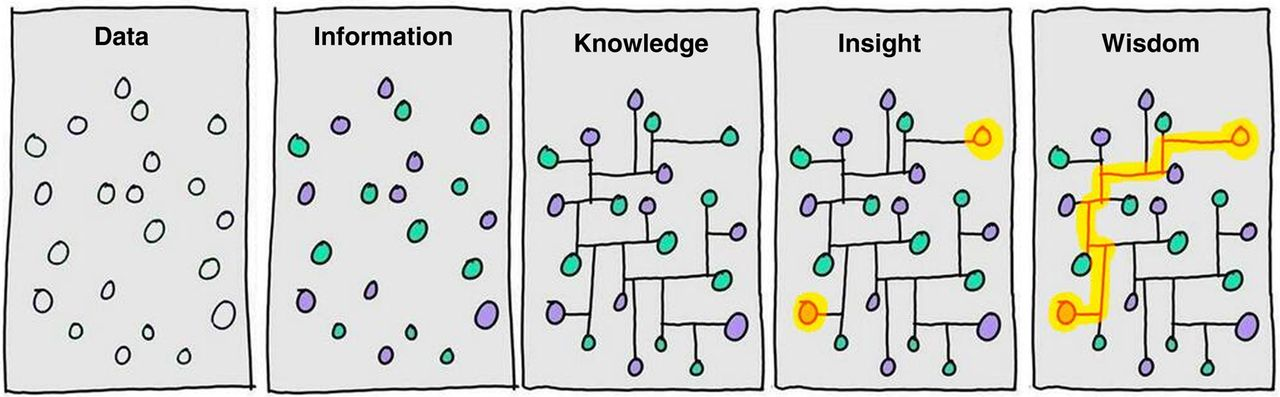
\includegraphics[width=0.8\linewidth]{figures-ext/01-Information_power} 

}

\caption[From Data to Wisdom]{\textbf{From \emph{Data} to
\emph{Wisdom}}. Illustration of different steps that it takes to go from
\emph{Data} to generating \emph{Wisdom}. It highlights that generating
data is not equal to understanding it and additional efforts are needed
to generate value. Image authored by Clifford Stoll and Gary Schubert
published by Portland Press Limited on behalf of the Biochemical Society
and the Royal Society of Biology and distributed under the
\href{https://creativecommons.org/licenses/by/4.0/}{Creative Commons
Attribution License 4.0 (CC-BY)} in \citep{Ponting2017}.}\label{fig:information-power}
\end{figure}











As discussed with the previous section cell-types, but also the whole
systems can be described at different levels (along different axes).
These different levels demand distinct technologies and strategies to be
developed to enable the measurements. For instance, a phenotypic
distinction between cells can be reached using FACS technology, for
molecular profiles omic methods were developed and for ultrastructure
microscopic methods. We need to approach biological systems from
different angles as no one of these axis provide a complete picture of
the studied system.

I will introduce most relevant data types that are used to study immune
infiltration of tumors.

\hypertarget{facs}{%
\subsection{Cell sorting}\label{facs}}

\hypertarget{flow-cytometry}{%
\subsubsection{Flow cytometry}\label{flow-cytometry}}

Flow cytometry is a laser-based technology. It uses marker genes: cell
surface proteins to sort cells in different compartments. Nowadays, it
permits quantification of the abundance of up to 17 cell surface
proteins using fluorescently labeled antibodies \citep{Papalexi2017}.
However this techniques is not free from bias, our knowledge about cell
markers is limited and several markers may not be relevant in some
context. Moreover, the scientific community did not clearly agree on the
marker choice even for popular and well-studied cell types which
introduced additional heterogeneity when independent studies are
compared. Also, the quality of antibodies may influence the results of
the FACs analysis. Besides those limitations FACs remains quite a
popular method for analyzing cells in complex tissues. It was among
first methods that allowed molecular phenotyping of immune cells, a
discovery of numerous subsets and their further functional
interpretation.

\hypertarget{mass-cytometry}{%
\subsubsection{Mass cytometry}\label{mass-cytometry}}

Mass cytometry (also known as CyTOF allows for the quantification of
cellular protein levels by using isotopes. It allows to quantify up to
40 proteins per cell \citep{Papalexi2017}. It also demands lower
starting number of cells (1000 - 1000000), a realistic number that can
be extracted from patient biopsy \citep{Lyons2017}.

\hypertarget{staining}{%
\subsection{Microscope Staining}\label{staining}}

Using microscope technics, histopathological cuts are analyzed. The
number of cells per a unit of area (i.e.~mm\(^2\)) is defined either
manually by a human or through diverse image analysis algorithms.

Current pathology practice utilizes chromogenic immunohistochemistry
(IHC) \citep{RamosVara2010}. Multiplexed approaches allow identifying
multiple markers in the same histopathology cut. Modern techniques like
imaging mass cytometry using FFPE tissue samples uses fluorescence and
mass cytometry to identify and quantify marker proteins
\citep{Giesen2014}.

The main advantage of aforementioned technics the number of cells that
can be analyzed and the information about the spatial distribution of
the different cell types. The limiting factor, as for
\protect\hyperlink{facs}{cell sorting methods}, is the number of markers
(\textasciitilde{}10-100) and consequently a number of cell types that
can be identified \citep{Schelker2017}.

The \protect\hyperlink{facs}{cell sorting methods} and
\protect\hyperlink{staining}{microscope staining} are usually considered
as a gold standard for multidimensional data techniques. The reason why
they are not applied at large scale is the cost but also quite laborious
and time-consuming sample preparation demanding a fresh sample. In
contrast, the \protect\hyperlink{omics}{omics methods} propose a more
scalable way to measure tumor microenvironment.

\hypertarget{tissue-microarrays}{%
\subsubsection{Tissue Microarrays}\label{tissue-microarrays}}

Tissue Microarrays aim to automatize ``staining'' techniques. A large
number of small tissue segments can be organized in a single paraffin
block where 100 tissue samples can be easily examined on one slide. A
variety of molecular or microscopic method can be then applied to FFPE
tissue including immunohistochemistry, FISH, and in situ hybridization
\citep{Wilczynski2009}. It is a technique in between traditional imaging
and omic high-throughput.

\hypertarget{omics}{%
\subsection{omics}\label{omics}}

In biological systems information is coded in the form of DNA that do
not vary a lot between different individuals of the same species. To
trigger a function in an organism, a part of the DNA is transcribed to
RNA, depending on the intrinsic and extrinsic factors, and after
additional modification messenger RNA (mRNA) is translated into a
protein (i.e., digestive enzyme) that fulfill a role in the organism.
The mRNA information (also called transcriptome) can be captured with
experimental methods at high throughput (transcriptomics) and provides
an approximation of the state of the studied system (i.e., a tissue).
There is also information, not coded on the DNA sequence but in a
pattern of chemical species that can regulate the state transition of
DNA information. These additional regulators are called epigenome
collectively and some of them, like methylation, can also be measured at
high-throughput.

\hypertarget{transcriptome}{%
\subsubsection{Transcriptome}\label{transcriptome}}

Transcriptomics measures the number of counts of mRNA molecules using
high-throughput techniques. mRNA is the part of the genetic information
that should be translated into proteins. It reflects the activity of
ongoing processes in a cell. In contrast to DNA, mRNA concentration can
be highly variable \citep{Velculescu1997}. This variability can be
either ``intrinsic'' that reflect the stochastic process of cell
machinery or ``extrinsic'' reflecting impact of factors upstream to mRNA
synthesis \citep{Satija2014}.

Transcriptome can be measured by microarrays or RNA-seq NGS technology.
Microarrays remain cost-efficient and popular technique designed in 90.
There exist two and one fluorescent color probes, both representing
different challenges in experimental design for batch effect removal.
RNA-seq, in contrast, uses sequenced RNA to quantify the expression. As
not only selected genes (probes) are quantified, it can be used to study
unknown parts of the genome. RNA-seq is also characterized by lower
background noise than microarrays.

Bulk transcriptome data are quite accessible nowadays. They can be
obtained from either flash-frozen or formalin-fixed, paraffin-embedded
(FFPE) tissue samples, including both surgically resected material and
core needle biopsies \citep{Schelker2017}.

The main flaw of transcriptomic data is that the reproducibility between
different platforms is limited. As a result, direct comparison (direct
merging, statistical difference tests) between two datasets produced by
different platforms is not advised. There are 12 thousand genes that are
matching between four sequencing platforms. Through gene names
conversions much information is lost, and bias is introduced.

Different strategies can be adapted to analyze bulk transcriptome.

\citet{Cieslik2017} describes five groups of most popular approaches
that can be applied to study transcriptome (Fig.
\ref{fig:transcriptome-methods}). Despite a diversity of bioinformatic
and statistical tools, the most popular differential approaches, mainly
differential gene expression (DGE) based on the difference between two
experimental conditions.

\begin{figure}

{\centering 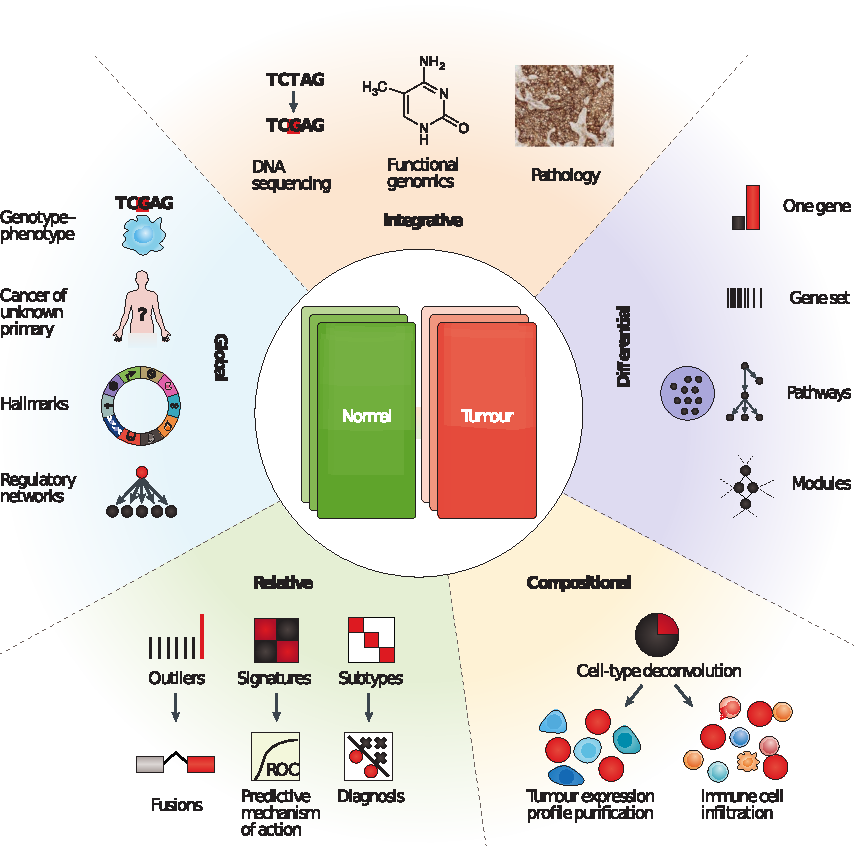
\includegraphics[width=1\linewidth]{figures-ext/transcriptome-methods} 

}

\caption[Five categories of RNA-seq data analysis.]{Five categories of RNA-seq data
analysis. Differential analyses: comparing two (or more) conditions,
Relative analyses: comparing to an internal reference (average, base
level), Compositional analyses: inferring cell types or groups of cell
types (i.e., tumor purity), Global analyses: pan-tissue and pan-cancer
analyses and Integrative analyses: compiling heterogeneous data types.
Reprinted by permission from Springer Nature \citep{Cieslik2017} © 2018
Macmillian Publishers Limited, part of Springer Nature. All rights
reserved.}\label{fig:transcriptome-methods}
\end{figure}











RNA-seq data was proven to be a useful indicator for clinical
applications \citep{Mody2015, Oberg2016, Robinson2017}. Its utility for
immune profiling was demonstrated in many studies through the use of
transcriptomic signatures to predict immunotherapy response or survival
\citep{Chen2016}.

In this work transcriptome data analysis falls into multiple categories:
Compositional, Relative and aims to construct Global-level conclusions.

\hypertarget{single-cell-rna-seq}{%
\subsubsection{Single cell RNA-seq}\label{single-cell-rna-seq}}

Described above methods of process DNA from hundreds of thousands of
cells simultaneously and report averaged gene expression of all cells.
In contrast, scRNA-seq technology allows getting results for each cell
individually. This is tremendous step forward enhancement of our
understanding of cell heterogeneity and opens new avenues of research
questions.

Continuous discovery of new immune subtypes has proven that cell surface
markers that are used for phenotyping by techniques like FACS and
immunohistochemistry cannot capture the full complexity. ScRNA-seq
methods allow clustering known cell types in subpopulations based on
their genetic features. ScRNA-seq is also able to capture particularly
rare cell types as it requires much less of RNA material (1 ng isolated
from 100-1000 cells) compared to `bulk' RNA-seq ( \textasciitilde{} 1 μg
of total mRNA transcripts ). It also allows studying cells at high
resolution capturing the phenotypes in much more refined scale than
previously \citep{Papalexi2017}.

This new data type also brings into the field new challenges related to
data processing due to the volume, distribution, noise, and biases.
Experts highlight as the most ``batch effect'', ``noise'' and ``dropout
effect'' \citep{Perkel2017}. So far, there are no official standards
that can be applied which makes data comparison and post-processing even
more challenging. Up to date, there are around 70 reported tools and
resources for single cell data processing \citep{Davis2016}. A limited
number of single-cell datasets of tumors are made publicly available,
and more are to come.

One can ask why then developing computational deconvolution of bulk
transcriptome if we can learn relevant information from single-cell
data. Firstly, that single cell data do not provide a straightforward
answer to the estimation of cell proportions. The coverage is not full
and sequenced single cells are not entirely representative of the actual
population. For instance, neutrophils are not found in scRNA-seq data
because of they are ``difficult to isolate, highly labile ex vivo and
therefore difficult to preserve with current single-cell methods''
\citep{Schelker2017}. Besides, a number of patients included in
published studies of range \textless{}100 cannot be compared to thousand
people cohorts sequenced with bulk transcriptome methods. This is mostly
because single cell experiments are challenging to perform, especially
in a clinical setting as fresh samples are needed \citep{Schelker2017}.
Today, single cell technology brings very interesting ``zoom in''
perspective, but it would be incautious to make fundings from a
restricted group of individuals universal to the whole population.
Primary brake to the use of single cell technology more broadly might be
as well the price that is nearly 10x higher for single cell sample
compared to bulk \citep{Cedar2018}.

In this work, we are using single cell data in two ways. Firstly, in
Chapter 5 we compare immune cell profiles defined by scRNA-seq, blood
and blind deconvolution (problem introduced in Immune signatures
section). Secondly, in Chapter 6 we use single call data of Metastatic
melanoma generated by \citet{Tirosh2016} to demonstrate heterogeneity of
subpopulations of Macrophages and NK cells.

\hypertarget{epi}{%
\subsubsection{Epigenome}\label{epi}}

An epigenome can be defined as a record of the chemical changes to the
\textbf{DNA and histone proteins} of an organism. Changes to the
epigenome can provoke changes to the structure of chromatin and changes
to the function of the genome \citep{Bernstein2007}. Epigenome data
usually contains information about methylation \textbf{CpG island
changes}. In cancer, global genomic hypomethylation, CpG island promoter
hypermethylation of tumor suppressor genes, an altered histone code for
critical genes, a global loss of monoacetylated and trimethylated
histone H4 were observed. Methylome profiles can also be used as a
molecular signature of disease and potential diagnostic or predictive
biomarker \citep{Jeschke2017}.

\hypertarget{copy-number-variation-cnv-and-copy-number-aberration-cna}{%
\subsubsection{Copy number variation (CNV) and Copy number aberration
(CNA)}\label{copy-number-variation-cnv-and-copy-number-aberration-cna}}

The differences between human genome come in the majority from
\textbf{Copy Number Variation }\citep{McCarroll2007}. CNV regions
constitute ~4.8--9.7\%~ of the whole human genome \citep{Zarrei2015}.
They can be reflected in structural variation that is duplication or
deletion of DNA bases. CNV can affect a lot of base pairs of DNA code
(deletion of more than 100 genes) and result in a phenotype change.

In addition, there can be distinguished, \textbf{Copy number
alterations/aberrations (CNAs)}~that are changes in copy number that
have arisen in~\textbf{somatic}~tissue (for example, just in a tumor),
in contrast to~CNV that~originated from changes in copy number
in~\textbf{germline}~cells (and are thus in all cells of the organism)
\citep{McCarroll2007}. CNV and CNA profiles can be associated with
diseases or cancer subtypes.

There exist disease-related exome panels that focus on regions with high
copy variation, or the full exome can be sequenced using whole-exome
sequencing (WES) \citep{Yamamoto2016}.

\hypertarget{spatial-transcriptomics}{%
\subsubsection{Spatial transcriptomics}\label{spatial-transcriptomics}}

\begin{quote}
Spatial transcriptomics provides quantitative gene expression data and
visualization of the distribution of mRNAs within tissue sections and
enables novel types of bioinformatics analyses, valuable in research and
diagnostics \citep{Stahl2016}
\end{quote}

It combines RNA-seq technology with spatial labeling which allows having
a bulk gene expression of 10-20 cells with given space coordinates
within the sample. It allows to localize regions of highest gene
expression and perform \emph{Spatially Variable Genes}
(\citet{Svensson2018}). Some attempts were already made to combine
Spatial Transcriptomics and scRNA-seq \citep{Moncada2018}. It remains an
early-stage technique, and so far it is not widely used, but it might be
a future of omics to add spatial information as it can be essential for
many research problems.

\hypertarget{immunotherapies}{%
\section{From cancer phenotyping to immune
therapies}\label{immunotherapies}}

This section outlines different methods of cancer immune phenotyping and
progress in cancer therapies with a focus on immune therapies. It will
link the ongoing research on TME with therapeutical potential.

\hypertarget{cancer-immune-phenotypes}{%
\subsection{Cancer immune phenotypes}\label{cancer-immune-phenotypes}}

Since 20s century physicians decided on common nomenclature that
classifies tumors into distinct groups that are relatively homogenous or
that share common characteristic important for treatment and prognosis.
Tumor typing should help to predict prognosis better, to adopt a therapy
to the clinical situation, to enable therapeutic studies which are
essential in proving any therapeutic progress.

Most of the classifications are based on clinical data. Most common
factors taken into account are the degree of local invasion, the degree
of remote invasion, histological types of cancer with specific grading
for each type of cancer, possibly various tumor markers, general status
of the patient.

However, cancers with similar morphological and histopathological
features reveal very distinct patterns of progression and response to
therapy \citep{Galon2014}. In the era of gene sequencing, gene and
protein expression, as well as epigenome, can provide valuable
complementary information. Therefore gene markers or proteomic
abnormalities can be integrated into classification panel. One famous
example is a gene signature \emph{PAM50} \citep{Parker2009} used for
prediction of patients' prognosis in breast cancer, patented as a tumor
profiling test.

Since the increase of importance of the immunotherapies, researches
proposed several ways to classify tumors based on their
microenvironment. Given different parameters describing TME, cancers can
be sorted into groups that show similar characteristics. We will discuss
most common frameworks that allow for phenotype cancers based on the
TME.

The localization of the immune cells can be an indicator of the state
and response to the therapy \citep{Bindea2013}.

The most standard approach is to convey an analysis of histopathological
cuts to asses the number of infiltrating lymphocytes (TILs). Two typical
patterns are usually identified: ``hot'' - immune inflamed and ``cold''
- no active immune response \citep{Berghoff2018}.

\citet{Chen2017} describe classification into inflamed and non-inflamed
tumors, where non-inflamed phenotypes: can be further split into the
immune-desert phenotype and the immune-excluded phenotype (Fig.
\ref{fig:immune-phenotypes}). The inflamed phenotype is characterized by
the abundant presence of immune cells: T cells, myeloid cells, monocytes
in tumor margin. Along with the immune cells, due to their
communication, a high expression of cytokines is characteristic for this
phenotype. According to \citet{Chen2017}, this is a mark that an
anti-tumor response was arrested by the tumor. The inflamed phenotype
has shown to be most responsive to immunotherapies. In the
immune-excluded phenotype, the immune cells are present as well but
located in the stroma \citep{Herbst2014}, sometimes penetrating inside
the tumor. However, when exposed to checkpoint immunotherapy, T cells do
not gain the ability to infiltrate the tumor; therefore the treatment is
inefficient. The immune-desert main features are little or no presence
of immune cells, especially T cells. Surprisingly, these tumors have
been proven to respond rarely to the checkpoint therapy
\citep{Herbst2014}. In non-inflamed tumors, cytokines associated with
immune suppression or tolerance are expressed.

\begin{figure}

{\centering 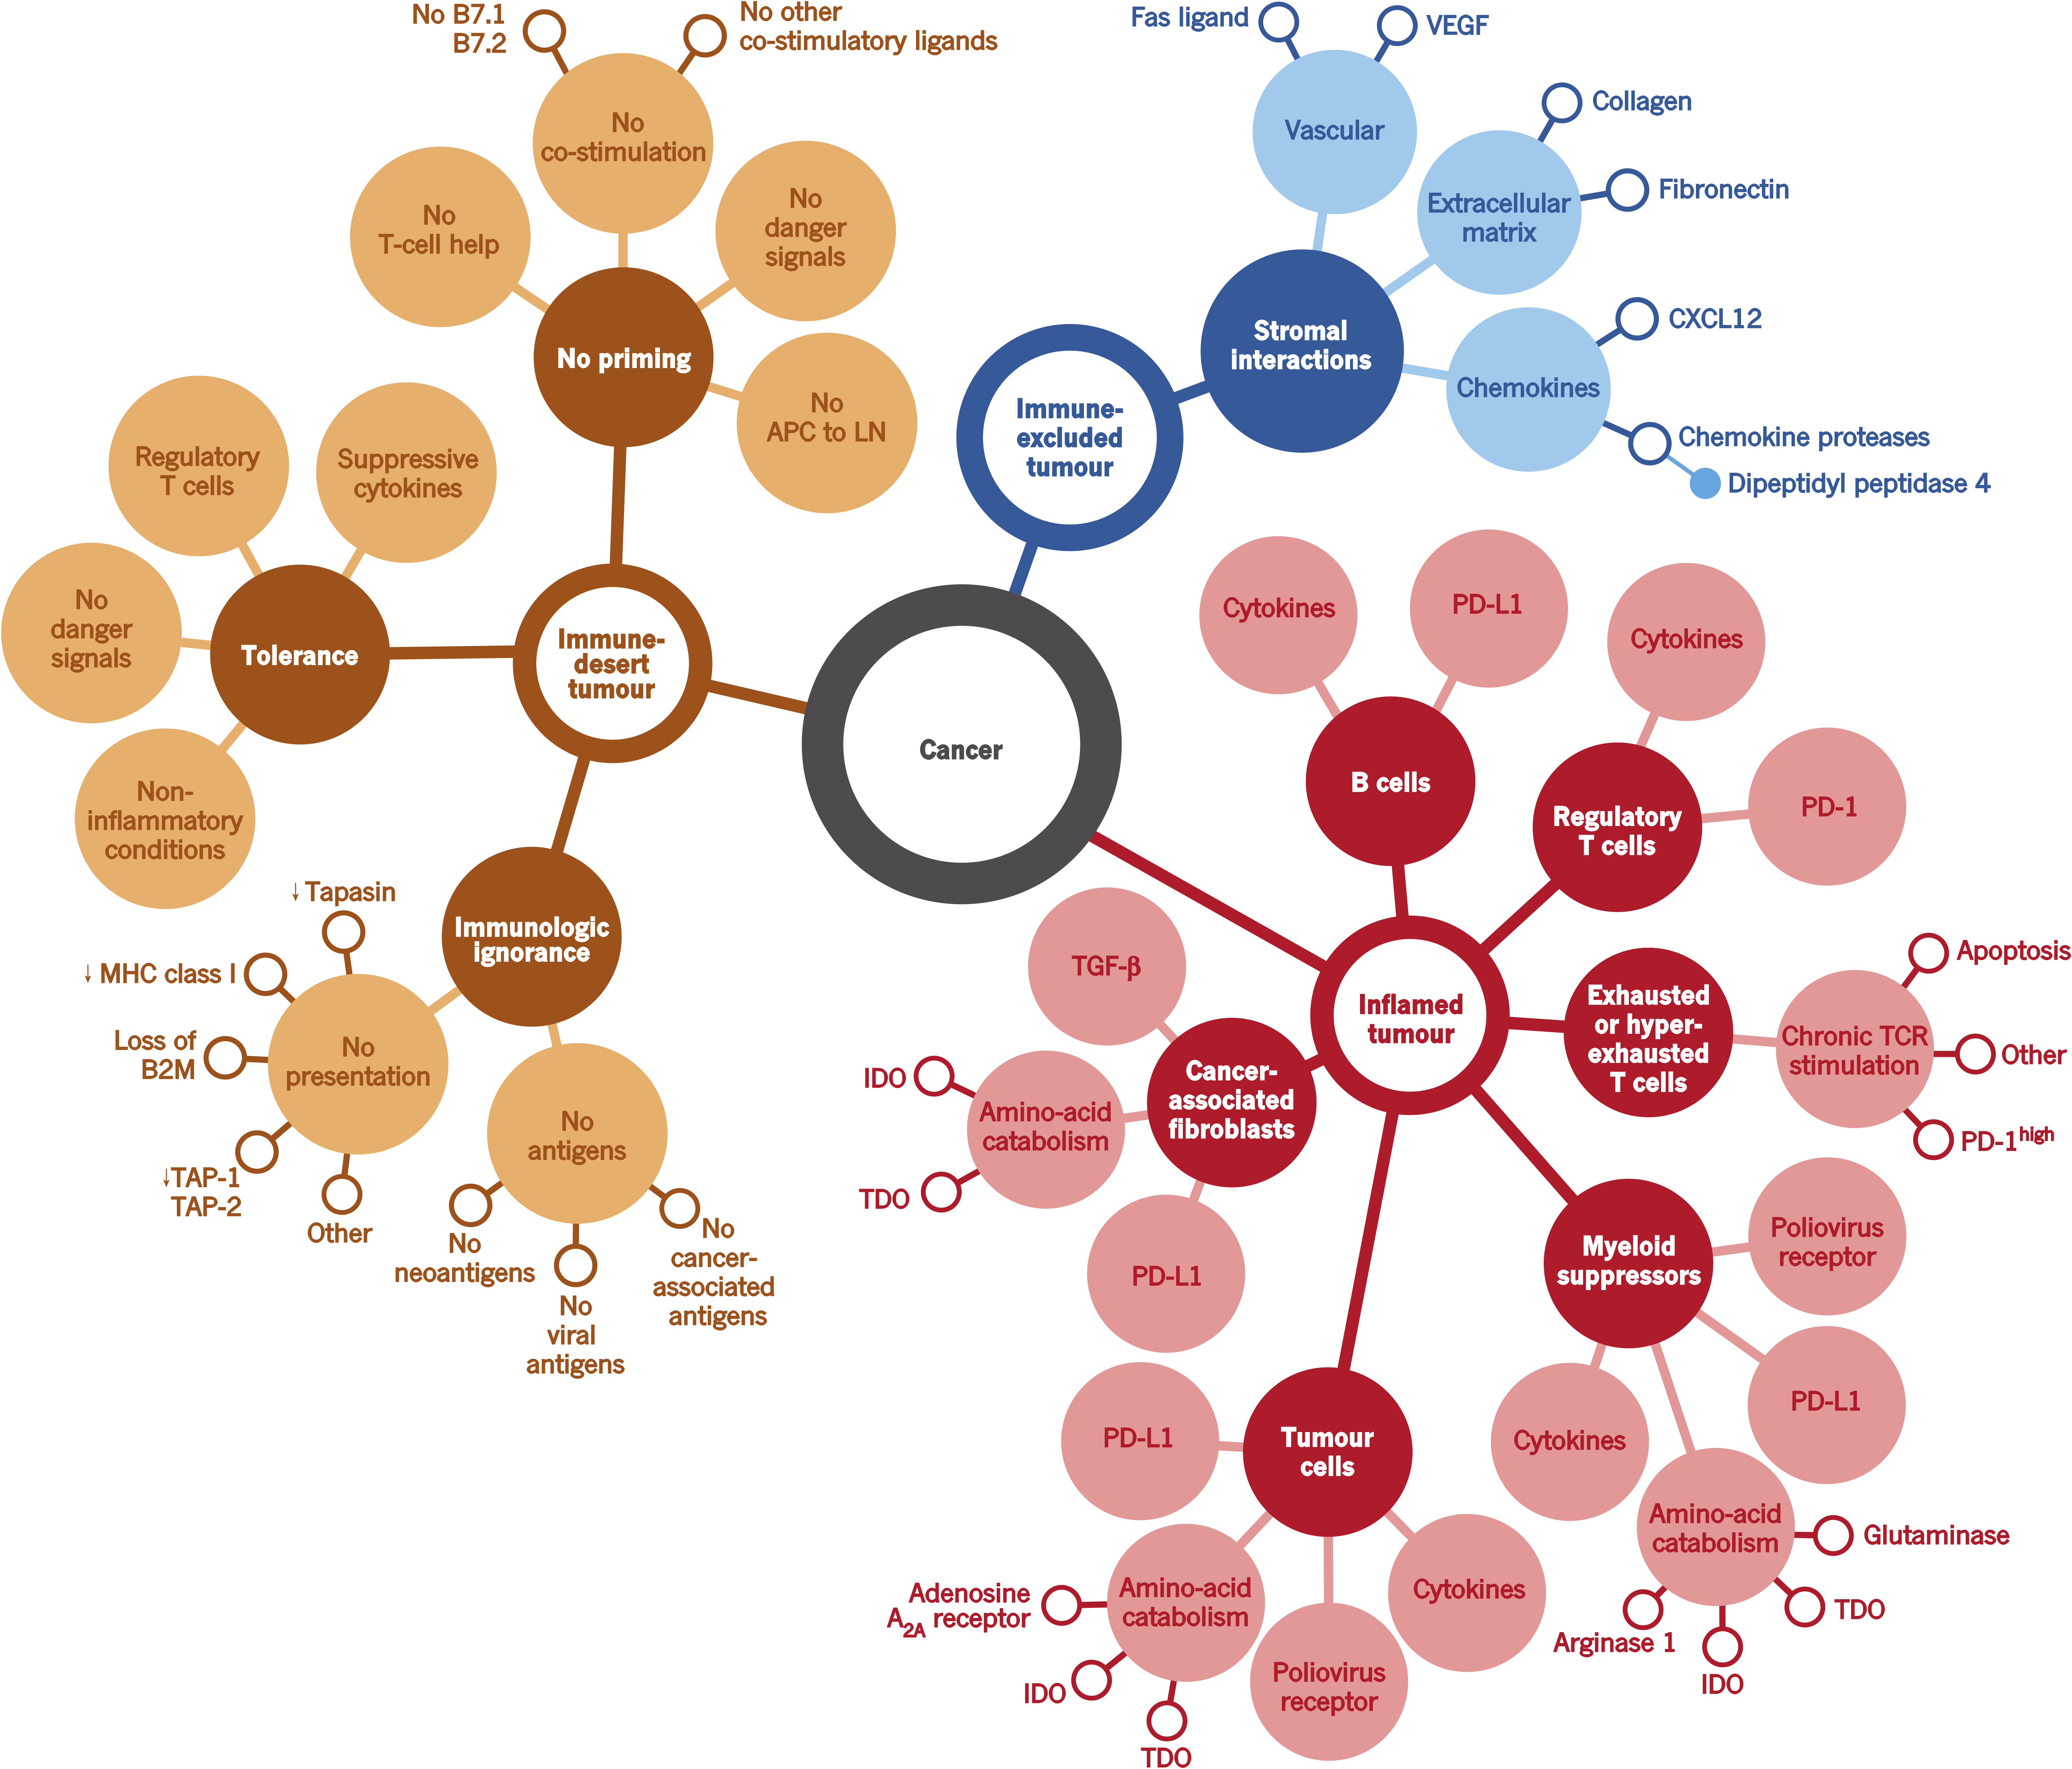
\includegraphics[width=1\linewidth]{figures-ext/immune-phenotypes} 

}

\caption[Cancer-immune phenotypes: the immune-desert phenotype, the immune-excluded phenotype and the inflamed phenotype.]{\textbf{Cancer-immune phenotypes: the
immune-desert phenotype (brown), the immune-excluded phenotype (blue)
and the inflamed phenotype (red).} The immune-desert phenotype is
characterized by a paucity of immune cells and cytokines. In the
immune-excluded phenotypes, the T cells are often present but trapped in
the stroma, enabled to migrate to the tumor site. The immune-inflamed
phenotype is rich in immune cells and the most responsive to the immune
checkpoint therapies. Reprinted by permission from Springer Nature
\citep{Chen2017} © 2017 Macmillian Publishers Limited, part of Springer
Nature. All rights reserved.}\label{fig:immune-phenotypes}
\end{figure}












A presence of immune phenotypes was confirmed by for example by
\citet{Becht2016} in colorectal cancer, where after deconvolution of
bulk tumor profiles, patterns of immune and stromal cells abundance was
matching four cancer subtypes. The good prognosis was related to
cytotoxic response and bad prognosis to lymphocytes and cells of
monocytic origin.

According to \citet{Gajewski2006}, the immunogenicity of the tumors can
be explained by tumor-intrinsic factors and tumor-extrinsic factors.
Tumor-intrinsic factors are the neoantigen load and frequency, the
mutational load, the expression of immunoinhibitors and
immunostimulators (e.i. PD-L1), and alteration of HLA class I molecules.
Tumor-extrinsic factors include chemokines regulating T cell
trafficking, infiltration of effector TILs and immunosuppressive TILs,
and soluble immunomodulatory factors (cytokines).

\hypertarget{scoring-the-immune-infiltration}{%
\subsection{Scoring the immune
infiltration}\label{scoring-the-immune-infiltration}}

Experimental techniques and computational tools enabled us to
characterize and classify TME with multi-omics data. Here I present
\textbf{a short list of most recent and influencing} analysis aiming to
redefine tumor phenotypes based on the immune infiltration, with a focus
on computational techniques.

\hypertarget{immunoscore}{%
\subsubsection{Immunoscore}\label{immunoscore}}

Jerôme Galon lab in Paris authors one of the most recognized scoring
method, based on fluorescent images and names
\href{http://www.haliodx.com/clinical-research-services/immunoscorer/}{Immunoscore}.
The Immunoscore ranges from 0 to 4 and it is based on the density of
lymphocyte populations CD3/CD45RO, CD3/CD8, or CD8/ CD45RO. It also
takes into account the spacial position of the cells: the tumor core and
margins \citep{Galon2012}. It was successfully applied to colorectal
cancer to predict patients' survival \citep{Anitei2014}. Since then, it
resulted in numerous application to many cancer types. Immunoscore has
been recently validated in a large cohort international independent
study (14 centers in 13 countries) as a relevant prognostic score of
time to recurrence, defined as the time from surgery to disease
recurrence \citep{Pages2018}.

The immunoscore is an interesting indicator, especially in the scope of
clinical applications, although it does not tell us a lot about
underlying biology. It is also limited to a few cell types while it may
be that in some cancer types or patients, the system requires more
detailed or rich analysis of a larger panel of cells.

\hypertarget{spatiotemporal-dynamics-of-intratumoral-immune-cells-of-colorectal-cancer}{%
\subsubsection{Spatiotemporal dynamics of Intratumoral Immune Cells of
Colorectal
Cancer}\label{spatiotemporal-dynamics-of-intratumoral-immune-cells-of-colorectal-cancer}}

\citet{Bindea2013} published a quite complete, and supported with strong
experimental evidence, immune landscape of colorectal cancer. Authors
introduced \emph{the immunome compendium} containing 577
cell-type-specific genes, derived from analysis of a significant corpus
of publicly available data. They used it to analyze CRC large
transcriptomic data (105 patients). Using qPCR (more sensitive technique
than microarray) expression of 81 ``representative'' genes from the
compendium was investigated in 153 CRC patients. This study validated
correlation of markers of the same type and also revealed the
correlation of different cell-type markers (i.e., T-cells and NK or Th
and macrophages). The data matrix was grouped into 3 clusters which were
corresponding to 1) tumor 2) adaptive 3) innate immune responses.
Besides, spatial positioning of markers was visualized thanks to Tissue
Microarray technology in samples from 107 CRC patients distinguishing
marker densities in tumor center and tumor margin areas. This was
followed by an in-depth study of chemokines expression and genomic
alterations. Also, authors validated potential prognostic biomarkers in
murine orthotopic CRC models.

In summary, using marker genes measured and visualized with different
data types of CRC, a high inter-patient heterogeneity was observed.
Adaptive immunity cells were associated with the core of the tumor and
the innate ones with the tumor margin. A mechanism involving CXCL13, Tfh
cells, B cells and IL-21 was identified as associated with good
prognosis.

Authors suggest a dynamic dimension of the study which is in practice
comparison between tumor stages. It can be argued that used time scale
is too discrete and true dynamics cannot be reflected only along tumor
stages in different patients. It is extremely challenging to access
truly dynamic data for human tumor biopsies, but some efforts are made
in the direction of inclusion of sequential biopsies \citep{Knebel2017}
that allow better time resolution. In brief, the field is still waiting
for the landscape of TME truly dynamic in space and time.

\hypertarget{immunophenoscore}{%
\subsubsection{Immunophenoscore}\label{immunophenoscore}}

Different approaches, sub-typing oriented, are based principally on gene
expression patterns. Most commonly, machine learning supervised
algorithms are trained to match known phenotype (established with
microscopy or with clinical features) to genetic patterns, or an
unsupervised clustering is used to discover new classification.

An example of well-formulated classification framework is
Immunophenoscore \citep{Charoentong2017}, based on the publication of
\citet{Angelova2015}, where methylome, transcriptome and mutation of
TCGA CRC dataset (n = 598) was used to describe \emph{immunophenotypes}.
Later on, it was reduced to gene expression indicator and summarised in
the form of a score. This scoring scheme is based on the data of 20
solid tumors, using the expression of marker genes selected by a machine
learning algorithm (random forest) for best prediction in each cancer.
These indicators can be grouped into four categories:

\begin{itemize}
\tightlist
\item
  MHC molecules (MHC)
\item
  Immunomodulators (CP)
\item
  Effector cells (EC)
\item
  Suppressor cells (SC)
\end{itemize}

The immunophenscore (IPS) is calculated on a 0-10 scale based on the
expression of genes in each category. Stimulatory factors (cell types)
impact the score positively and inhibitory factors (cell types)
negatively. Z-scores \(\geq\) three were designated as IPS10 and
z-scores \(\leq\) 0 are designated as IPS0. A similar conceptual
framework called \emph{cancer immunogram} was proposed by
\citet{Blank2016} included seven parameters: tumor foreignness
(Mutational load), general immune status (Lymphocyte count), immune cell
infiltration (Intratumoral T cells), absence of checkpoints (PD-L1),
absence of soluble inhibitors (IL--6, CRP), absence of inhibitory tumor
metabolism (LDH, glucose utilisation), tumor sensitivity to immune
effectors (MHC expression, IFN-\(\gamma\) sensitivity).
\citet{Charoentong2017} claim that the immunophenoscore can predict
response to CTLA-4 and anti-PD-1.

Nonetheless, the details of the use of \emph{cancer immunogram} in
practice remain unclear and the result could be sensitive to patients'
and data heterogeneity as no standardization was proposed. It should
also be validated in a systematic, independent study.

\hypertarget{the-immune-landscape-of-cancer}{%
\subsubsection{The immune landscape of
cancer}\label{the-immune-landscape-of-cancer}}

\rowcolors{2}{gray!6}{white}\begin{table}

\caption[Six immunological subtypes of cancer]{\label{tab:C6}\textbf{Six immunological subtypes of cancer}. The
general characteristic of subtypes generated by \citet{Thorsson2018} as
described in the original publication.}
\centering
\resizebox{\linewidth}{!}{
\begin{tabular}[t]{|>{}c|>{}c|>{}c|>{}c|>{}c|>{}c|>{}c|}
\hiderowcolors
\toprule
\rowcolor{Gray}  \textcolor{white}{\textbf{Cluster}} & \textcolor{white}{\textbf{Features}} & \textcolor{white}{\textbf{Macrophage..lymphocyte}} & \textcolor{white}{\textbf{Th1.Th2}} & \textcolor{white}{\textbf{Proliferation}} & \textcolor{white}{\textbf{Intratumoral.heterogeneity}} & \textcolor{white}{\textbf{Other}}\\
\midrule
\showrowcolors
C1 & Wound healing & Balanced & Low & High & High & \\
C2 & IFN-$\gamma$ dominant & Lowest & Lowest & High & Highest & Highest M1 and CD8 T cells\\
C3 & Inflammatory & Balanced & High & Low & Lowest & Highest Th17\\
C4 & Lymphocyte depleted & High & Minimal Th & Moderate & Moderate & \\
C5 & Immunologically quiet & Highest & Minimal Th & Low & Low & Highest M2\\
C6 & TGF-$\beta$ dominant & High & Balanced & Moderate & Moderate & Highest TGF-β signature\\
\bottomrule
\end{tabular}}
\end{table}\rowcolors{2}{white}{white}

\citet{Thorsson2018} performed a multi-omic analysis of TCGA datasets
that allowed them to define six subtypes that are valid across cancer
types (see Tab. \ref{tab:C6} ).





Authors selected eight indicators to define these six phenotypes:

\begin{enumerate}
\def\labelenumi{\arabic{enumi}.}
\tightlist
\item
  differences in macrophage or lymphocyte signatures
\item
  Th1:Th2 cell ratio
\item
  extent of intratumoral heterogeneity
\item
  aneuploidy
\item
  extent of neoantigen load
\item
  overall cell proliferation
\item
  expression of immunomodulatory genes
\item
  prognosis
\end{enumerate}

These indicators were selected among many other indicators though
machine learning (elastic net regression) for the best predictive power
of survival.

All the data and computed parameters can be accessed at
\href{https://isb-cgc.shinyapps.io/shiny-iatlas/}{CRI iAtlas Portal}.
Among the six phenotypes C3 (Inflammatory) has the best-associated
prognosis while C1 (wound healing) and C2 (IFN-\(\gamma\) dominant),
much less favorable outcome. This again illustrates the ambivalent
nature of the immune system as the best, and the worst prognosis is
associated with immunologically active tumors. C4 (lymphocyte depleted)
and C6 (TGF-\(\beta\) dominant) subtypes had the worst prognosis. The
content of immune cells was determined using different tools and data
types (expression, DNA methylation, images, etc.) We can learn a lot
from the study. However, it seems difficult to integrate the methods
into an ordinary practice because different data levels are necessary
for the same samples to compute all the indicators.

\hypertarget{a-pan-cancer-landscape-of-immune-cancer-interactions-in-solid-tumors}{%
\subsubsection{A pan-cancer landscape of immune-cancer interactions in
solid
tumors}\label{a-pan-cancer-landscape-of-immune-cancer-interactions-in-solid-tumors}}

A different classification was proposed by \citet{Tamborero2018}, also
using TCGA data. They distinguished 17 immune infiltration patterns
based on the immune cell proportions and 6 different clusters based on
cytotoxicity measure across all cancer types (named immune-phenotypes)
that were finally summarized in three groups: cytotoxic immune
infiltrate, infiltrate with more immune-suppressive component and poor
immune infiltrate. According to the analysis, one of the most critical
factors is cytotoxicity. Tumors with high cytotoxicity were
characterized by low clonal heterogeneity, with gene alterations
regulating epigenetic, antigen presentation and cell-cell communication.
The medium-level cytotoxic tumors had activated invasion and remodeling
of adjacent tissue, probably favorable to immune-suppressive cells. The
low cytotoxicity subgroup of tumors had altered: cell-cycle, hedgehog,
\(\beta\)- catenin and TGF-\(\beta\) pathways. This result roughly
overlaps with the one of \citet{Thorsson2018}. The survival analysis
based on the six immune-phenotypes revealed that for most cancer types,
high cytotoxic tumors are associated with better survival. To evaluate
tumor environment cells, authors used gene set variation analysis
\citep{Hanzelmann2013} with a set of pre-defined cell-type markers.
Another important conclusion of \citet{Tamborero2018} is that tissue of
origin is not the only important factor shaping cell-type patterns in
tumors. However, the least infiltrated tumors were lung, uterine and
bladder cancers, while the most infiltrated were pancreatic, kidney,
skin cancers and glioblastoma. They also analyzed cancer cell pathways
after computational purification of tumor samples (subtraction of the
immune signal) to better understand cancer signaling.

A different approach is to characterize tumors based on signaling
pathways organized in functional modules.

\hypertarget{immune-maps}{%
\subsubsection{Immune maps}\label{immune-maps}}

Another way to summarize tumor phenotype can be through the use of
molecular maps. \href{https://acsn.curie.fr/}{Atlas of Cancer Signaling
Network (ACSN)} \citep{Kuperstein2013, Kuperstein2015} is a pathway
database that contains a collection of interconnected cancer-related
signaling network maps. An additional feature is ACSN web-based
Google-maps-like visualization of the database. User data can be
projected on the molecular map (for example gene/protein expression from
user data can be paired with entities on the map ). ACSN 2.0 contains
Cancer cell map and TME map (at the time: angiogenesis, innate immune
map, T-cell signaling maps). All separate maps are available in
\href{https://navicell.curie.fr/pages/maps.html}{Navicell website}.
Through projection of the data on the innate immunity map, one can see
if a tumor sample is characterized by pro- or anti-tumor activated
pathways due to the organization of the map layout. Also, different CAF
subtypes were characterized by the CAF specific map in
\citep{Costa2018}. Kondratova and colleagues (including myself) used the
innate immune map to characterize NK and Macrophages subtypes
(\protect\hyperlink{map}{see Chapter Z}).

\hypertarget{summary-1}{%
\subsubsection{Summary}\label{summary-1}}

Despite all scientific efforts, the gene expression-based
classifications are not yet used in clinics. The measured multi-panel
mRNA expression, which can be included into the category of In Vitro
Diagnostic Multivariate Index Assay (IVDMIA)
\citep{Gyorffy2015, Ross2008}, may be a future of TME-based cancer
classification, diagnosis and treatment recommendation
\citep{Gnjatic2017}. For this best tools need to be used to evaluate the
state of TME and tumor-stroma-immune cells communication properly.

\hypertarget{immune-signatures}{%
\subsection{Immune signatures - biological
perspective}\label{immune-signatures}}

A gene signature is

\begin{quote}
\emph{a single or combined group of genes in with a uniquely
characteristic pattern of gene expression that occurs as a result of an
altered or unaltered biological process or pathogenic medical condition}
\citep{Itadani2008, Liu2008}.
\end{quote}

They can be classified based on their form:

\begin{itemize}
\tightlist
\item
  metagene
\item
  gene list
\item
  weighted gene list
\end{itemize}

A term \textbf{metagene} or \emph{eigen gene} describes an aggregated
pattern of gene expression. The aggregation can correspond to simple
mean of samples or can be obtained though matrix factorisation or source
separation techniques, clustering. A metagene usually provides values
for all measured genes (all probes) in contrast to a wighted gene list
where weights are associated with selected genes.

\textbf{Gene lists} are simple enumeration of transcripts names or gene
identifiers. Application of gene list is often limited to gene
enrichment analysis tools or gene selection from the data.

An alternative is a \textbf{weighted gene list} or ranked gene list,
where genes are ranked according to their importance. Often the ranks is
obtained though comparison between two conditions or test/control. They
can be also based on absolute gene expression values\citep{Lyons2017}.
One possible problem with this weighted gene list can be platform
dependence.

There exist a big choice of databases storing collections of signatures.
They contain gene expression and other genomic data such as genotype,
DNA methylation, and protein expression data attributed to some
condition of reference. A big collection of immune signatures are
regrouped by \href{https://www.immgen.org/}{Immunological Genome Project
(IGP, ImmGen)} \citep{Heng2008}. Gene expression of protein coding genes
measure in mice immune cells, ex vivo, in different conditions (drug
treatment, perturbations) were regrouped in this ressource. A different
ressource
\href{https://sysimm.ifrec.osaka-u.ac.jp/immuno-navigator/}{Immuno-navigator}
\citep{Vandenbon2016} that stores information about human and murine
immune genes and co-expression networks.
\href{http://software.broadinstitute.org/gsea/msigdb/collections.jsp}{ImmuneSigDB}
is a collection of gene-sets that describe immunity and inflammation in
transcriptomic data \citep{Godec2016} and a part of popular MSigDB
ressource used commonly for gene set enrichment analysis (GSEA)
\citep{Subramanian2005}.

They can also be classified based on their use:

\begin{itemize}
\tightlist
\item
  prognostic signatures
\item
  predictive signatures
\item
  diagnostic signatures
\item
  specific signatures
\end{itemize}

The \emph{prognostic} signatures can distinguish between patients with a
good or from patients with bad prognosis when deciding to assign a
patient to a therapy.

The \emph{predictive} signatures are able to predict treatment benefit
between experimental and/or nontraditional treatment groups vs.~control,
i.e.~in clinical trials \citep{Michiels2016}.

The \emph{diagnostic} signature, also called \emph{biomarkers} can be
used for detection of a disease in a patient, like for example in blood
tests.

The \emph{specific} signatures should describe with robustness and
reproducibility the same group of cells, or patients, or condition with
respect to other considered groups. For instance, in the context of
cell-types, among studied cell-types a specific signature will
distinguish only one cell type. In the context of cancer subtypes, it
will indicate clearly one subtype among others.

Examples of predictive and prognostic gene signatures, used in clinical
practice are Oncotype DX, EndoPredict, PAM50, and Breast Cancer Index
for breast cancer \citep{Harris2016}.

Studies discussed in this Chapter showed plausible importance of
immune-related signals in cancer therapy. However, there is no no
immune-related gene signatures used in clinical practice currently. This
can be because of the lack of consistency of genes, both within the same
tumor type and among different tumors that can be found in the
signatures \citep{Chifman2016}. Difference in gene expression of
different cell populations were found even intra- and interlabs. This
difference can be due to confounding factors like stress or to
contamination \citep{Heng2008}.

In many studies \emph{specifc} signatures of cell types are used. They
seem to be good in discriminating between broad lineages of cell type,
such as lymphoid and myeloid. Although thier capacity to describe cell
states and cell subtypes is more discutable \citep{Chifman2016}. Another
matter is that cell type signatures are often obtained in model
organisms or extracted from different tissue (i.e.~blood-derived
signatures vs cancer-derived signatures).

\begin{quote}
\emph{the gene expression profiles of tumour-associated immune cells
differ considerably from those of blood derived immune cells}
\citep{Schelker2017}
\end{quote}

With emergence of single-cell signatures, there are new horizons of gene
signatures to be discovered. Especially signatures of rare cell types in
solid tissues. Yet, it is up to researches to cross validate single cell
signatures with different types of data as scRNA-seq is not free of
platform and post-processing bias.

Immune signatures will be also discussed as a part of deconvolution
pipeline in the \protect\hyperlink{methods}{Chapter 2} under the section
about \emph{basis matrix} in mathematical terms.

\hypertarget{cancer_Therapies}{%
\subsection{Cancer therapies}\label{cancer_Therapies}}

Cancer is a complex disease. Up to date, no uniform and fully effective
treatment were proposed, and usually different strategies are tested to
kill tumor cells. \textbf{Surgery} is one of the oldest methods. The
cancer is removed from the patient body. There are different ways, more
or less invasive, that it can be performed. It is usually applied for
solid tumor contained in a small area. \textbf{Radiation Therapy} uses
high doses of radiation to eliminate tumor cells and shrink tumor mass.
It can be applied externally or internally. \textbf{Chemotherapy} uses a
drug (or a combination of drugs) that kill cancer cells, usually
altering cell proliferation and growth. The drawback of radiotherapy and
chemotherapy are substantial side effects. \textbf{Hormone therapy }
modulate hormone levels in the body in order to inhibit tumor growth in
breast and prostate cancers. In leukemia and lymphoma, can be applied
\textbf{stem cell transplants} that restore blood-forming stem cells
destroyed by the very high doses of chemotherapy or radiation therapy
that are used to treat certain cancers.

Alternatively, \textbf{targeted therapies} represent a more focused
strategy that aims to be more efficient and cause fewer side effects
than systematic therapies. Two main types of targeted therapies are
small-molecule drugs and monoclonal antibodies. Targeted therapies
usually aim to stimulate/inhibit a selected molecular function.
Particular types of targeted therapies are \textbf{Immunotherapies}.
Through activation/inhibition of immune regulatory pathways, it
stimulates the immune system to destroy malignant cells. A continuation
of targeted therapies is \textbf{precision medicine approach}. It is
based on genetic information to specify patient's profile and find a
suitable treatment. A number of innovative treatments targeting a
specific change in tumor ecosystem are being tested presently in
precision medicine clinical trials \citep{NCI2018}.

\hypertarget{recent-progress-in-immuno-therapies}{%
\subsection{Recent progress in
immuno-therapies}\label{recent-progress-in-immuno-therapies}}

The immunotherapies, in contrast with other types of cancers therapies
discussed in \protect\hyperlink{cancer_Therapies}{the previous section},
aim to trigger or restart the immune system to defend the organism and
attack the malignant cells without provoking persisting inflammation
state \citep{Predina2013}

The idea of stimulating the immune system to fight malignant cell was
not born recently. For a long time, a possibility of development of an
anti-cancer vaccine has been investigated. Unfortunately, this idea
faced two essential limitations 1) lack of knowledge of antigens that
should be used in a vaccine to stimulate cytotoxic T cells successfully)
the ability of cancer to block the immune response also called
\emph{immunostat}. Despite those impediments works on anti-tumor
vaccines do not cease \citep{Palucka2013}. A very recent promising an
in-situ anti-tumor vaccine was proposed by Sagiv-Barfi et al.
\citep{Sagiv-Barfi2018}. The therapy tested in mice would be based on
local injections of the combination of ``unmethylated CG-enriched
oligodeoxynucleotide (Cp-G) - a Toll-like receptor 9 (TLR9) ligand and
anti-OX40 antibody. Low doses of CpG injected into a tumor induce the
expression of OX40 on CD4+ T cells in the microenvironment in mouse or
human tumors. An agonistic anti-OX40 antibody can then trigger a T cell
immune response, which is specific to the antigens of the injected
tumor''. Sagiv-Barfi et al.~claim this therapy could be applied to all
tumor types, as long as they are leucocyte-infiltrated. As a local
therapy, in situ vaccination should have fewer side-effects than
systematic administration. It is now undergoing clinical trials to test
its efficiency in human patients.

Another idea involving using the immune system as a weapon to fight
cancer would be the use of genetically modified patient's T-cells,
carrying \emph{CARs} (chimeric antigen receptors) \citep{Jackson2016}.
After an extended period of small unsuccessful trials, recently in 2017,
two CAR T-cell therapies were accepted, one to ``treat adults with
certain type of large B-cell lymphoma'' \citep{FDACARTadult}, other to
treat ``children with acute lymphoblastic leukemia (ALL)''
\citep{FDACARTALL}, which are, at the same time, the first two gene
therapies accepted by FDA.

However, the two most promising immuno-related strategies with proven
clinical efficiency are based on blocking so-called immune checkpoint
inhibitors: cytotoxic T-lymphocyte protein 4 (CTLA4) and programmed cell
death protein 1 (PD-1). The anti-CLTA4 antibodies blocks repressive
action of CLTA4 on T-cells and they become therefore activated. It was
shown efficient in melanoma patients and accepted by FDA in 2015 as
adjuvant therapy for stage III metastatic melanoma patients
\citep{FDACTLA4}. PD-1 is a cell surface receptor of T cells, that binds
to PD-L1/PD-L2. After binding, an immunosuppressive pathway is activated
and T cells activity is dampened. An action of an anti-PD-L1 antibody is
to prevent this immune exhaustion \citep{Chen2017}. A stepping stone for
anti-PD-L1 therapies was approval of Tecentriq (atezolizumab) for
Bladder cancer \citep{FDAPDL1Bladder} and anti-PD1 Keytruda
(pembrolizumab) initially accepted for NSCLC and further extended to
head and neck cancer, Hodgkin's lymphoma, gastric cancer and
microsatellite instability-high cancer \citep{FDAPDL1NSCLC}. Since that
breakthrough, other anti-PD-L1 or anti-PD1 antibodies were accepted or
entered advanced stages of clinical trials \citep{Wolchok2015}. A short
history of immunotherapy FDA-accepted treatments can be found in Fig.
\ref{fig:timeline-immunotherapies}

\begin{figure}

{\centering 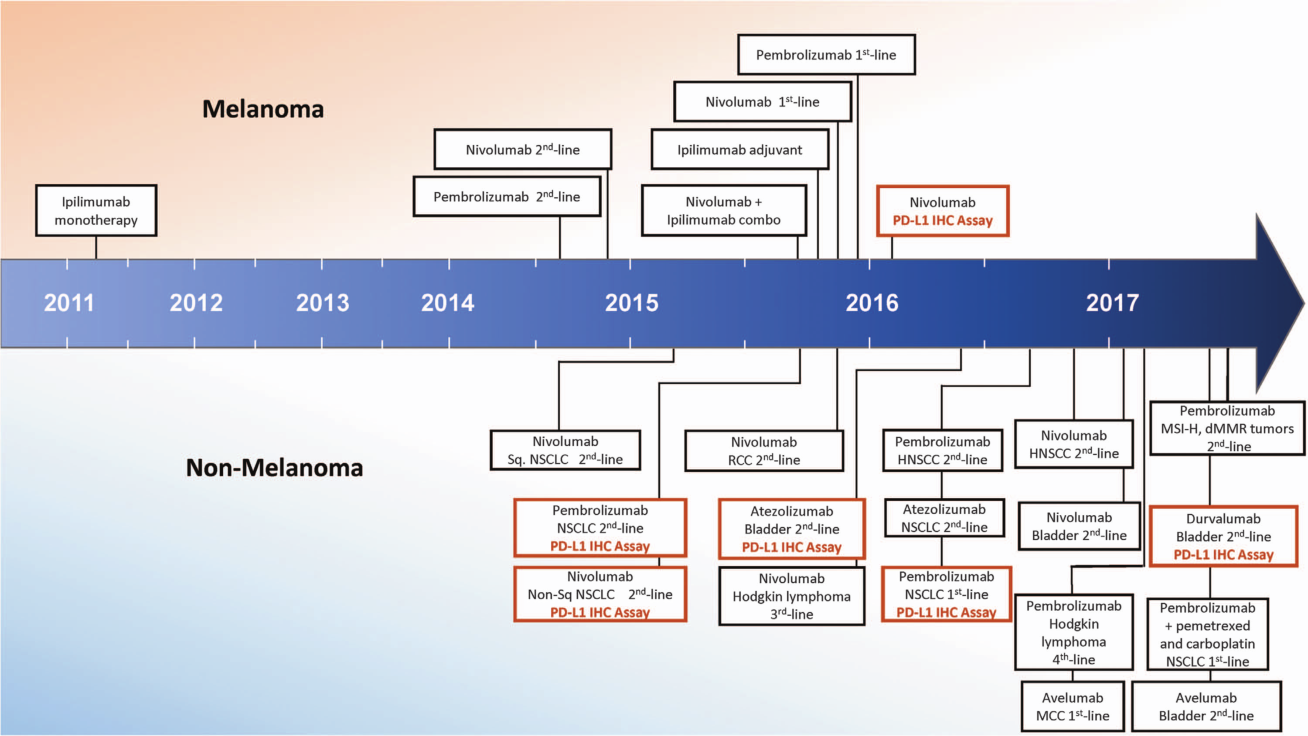
\includegraphics[width=1\linewidth]{figures-ext/02-timeline-immunotherapies} 

}

\caption[This timeline describes short history of FDA approval of checkpoint blocking immunotherapies up to 2017.]{\textbf{This timeline describes
short history of FDA approval of checkpoint blocking immunotherapies up
to 2017.} Reprinted by permission from Springer Nature
\citep{Taube2017a} Macmillan Publishers Limited, part of Springer
Nature. All Rights Reserved.}\label{fig:timeline-immunotherapies}
\end{figure}







The main drawback of immunotherapies is heterogeneity of response rate,
which can vary, i.e., from 10--40\% in case of PD-L1blocking
\citep{Zou2016}, suggesting that some patients can have more chances
than others to respond to immune therapy. So far, it has been shown that
anti PD-L1 therapies work more effectively in T cell infiltrated tumors
with the exclusion of Tregs because of lack of difference in expression
of FOXP3 in responding and the non-responding group of patients
\citep{Herbst2014}. Also, some light has been shade by \citet{Rizvi2015}
who connected mutational rate of cancer cells to the chances of response
to immunotherapy.

Despite those findings, the precise qualifications of patients that
should be sensitive to immunotherapy are not defined \citep{Pitt2016}.
As most patients do not answer to immunotherapies, it stimulates
researches to look for better biomarkers and patient stratifications,
and pharmaceutical industries to discover new immune checkpoints based
therapies.

\hypertarget{summary-of-the-chapter}{%
\section{Summary of the chapter}\label{summary-of-the-chapter}}

Cancer remains a critical health problem of our era that touches many
people. Tumor cells are interacting with their microenvironment (called
Tumor Microenvironment (TME)) including normal cell, stromal cells and a
variety of immune cells. These cells can have a role in disease
progression and response to treatment. A modern approach to modulate TME
was proposed through an application of immune therapies.

A new way to classify cancers based on their TME is called
immunophenotyping. Widely used TCGA data contains many different data
types, but not all of possible data types. Before entering a clinical
practice, the immunophenotyping approaches will need to face important
challenges. Would addition of a new data type (i.e., FACS) change the
patients classification? Can the similar results be found in
non-American patient cohorts? What if different technologies are used,
if data are not normalized uniformly, would it change the conclusions?
What if not all data types available in TCGA are not produced for other
patients? How these classification can be reproduced for smaller
cohorts? Can these complex classification schemes be reduced to a few
easy measurable indices? It is important to acknowledge the authors for
their remarkable work. However it is also crucial to remember we are
biased by the piece of the truth (type of data) we use, that can be on
the top biased with technical and experimental design.

To produce a very detailed system-level view of the TME with traditional
experimental techniques an uncountable amount of work and resources
would be necessary. Using omic techniques system approach is possible to
reduce the time and resources. However, to embrace fully the data
complexity, computational tools are indispensable. From the data
generation to the analysis, different statistical and mathematical
challenges need to be faced before arriving at valid biological results
and interpretations.

As I will present in the next chapter, in order to solve the problem of
extraction of cell-type heterogeneity from cancer bulk omic data, a
number of approaches were developed.

\hypertarget{methods}{%
\chapter{Mathematical foundation of cell-type deconvolution of
biological data}\label{methods}}

\chaptermark{Mathematical introduction}

In the previous chapter, I presented state-of-art of the current
immuno-oncology research that has to embrace the vast complexity of
cancer disease and the immune system. One part of this complexity can be
explained by the presence and quantities of tumor-infiltrating immune
cells, their interactions with each other and the tumor.

In this chapter, I will discuss how mathematical models can be used to
extract information about different cell-types from `bulk' omics data or
how to de-mix mixed sources composing the bulk samples. To start with, I
will introduce you to basic concepts of machine learning. Then I will
focus on approaches adapted for cell-type deconvolution. In a literature
overview, I will depict the evolution of the field as well as discuss
the particularities of different tools for estimating presence and
proportion of immune cells within cancer bulk omic data.

\hypertarget{introduction-to-supervised-and-unsupervised-learning}{%
\section{Introduction to supervised and unsupervised
learning}\label{introduction-to-supervised-and-unsupervised-learning}}

Machine learning (ML) is a field of computer science where a system can
learn and improve given an objective function and the data.

Mitchell gave a popular definition of machine learning in 1997:

\begin{quote}
Machine learning: \emph{A computer program is said to learn from
experience E with respect to some class of tasks T and performance
measure P if its performance at tasks in T, as measured by P, improves
with experience E}.

--- Mitchell in 1997 \citep{Mitchell1997}
\end{quote}

Term \emph{Artificial intelligence} (AI) is often used by the media or
the general public to describe machine learning. Indeed ML can be
considered as a branch of AI, together with computer vision and deep
neural networks applications. However, commonly ML and AI are used
interchangeably by the broad public.

ML is applied commonly in many fields of science and industry. I will
not discuss here subtle differences between machine learning,
statistical learning, computational statistics and mathematical
optimization.

In general, algorithms can be divided into groups given the application:

\begin{itemize}
\tightlist
\item
  classification - aims to assign observations to a group (discrete
  variable)
\item
  regression - aims to predict a continuous response of an input
  (continuous variable)
\item
  clustering - aims to divide data into groups that are related to each
  other based on a distance
\end{itemize}

Another critical distinction can be made given the inputs to the
algorithm. Here, I present the differences between supervised and
unsupervised learning.

\hypertarget{supervised-learning}{%
\subsection{Supervised learning}\label{supervised-learning}}

Supervised learning can be described as ``the analysis of data via a
focused structure'' \citep{Piegorsch}. The primary task is to predict an
output given the inputs. In the statistical language, the inputs are
often called the predictors or the independent variables. In the pattern
recognition literature, the term features are preferred. The outputs are
called the responses, or the dependent variables. \citep{Hastie2009}

The initial data is divided into two sets: training and test. First, the
model is trained with correct answers on the training data (learning to
minimize the error), and then its performance is evaluated on the test
data.

Among widely used classifiers there are Support Vector Machines (SVM),
partition trees (and their extension random forests), and neural
networks. For regression, it is common to encounter linear regression,
boosted trees regression,

\hypertarget{unsup}{%
\subsection{Unsupervised learning}\label{unsup}}

In Unsupervised learning is given the data and is asked to segment the
data given a particular constraint. However, the true segments of the
data are not known. Therefore an unsupervised algorithm aims to unveil
the ``hidden structure'' of the data or latent variables.

One group of unsupervised learning are descriptive statistic methods,
such as principal components, multidimensional scaling, self-organizing
maps, and principal curves. These methods aim to represent to the data
most adequately in low-dimensional space \citep{Hastie2009}.

Another group is clustering algorithms. Clustering is the way to create
groups (multiple convex regions) based on the intrinsic architecture of
the data. These groups are not necessarily known beforehand but can be
validated with the domain knowledge. Popular clustering algorithms are
k-means, hierarchical clustering, mixture density-based clustering
\citep{Xu2008}.

In both descriptive statistics and clustering, one important parameter
(i.e.~denoted \(k\)) is the number (number of factors, variables,
clusters) to which the data should be decomposed. Different algorithms
and applications can propose an automatic choice of \(k\) based on
formal indexes or previous knowledge, in others, the user needs to
provide the \(k\).

\hypertarget{low-dimensional-embeddingfor-visualization}{%
\subsection{Low-dimensional embedding~for
visualization}\label{low-dimensional-embeddingfor-visualization}}

There is a common confusion, often seen in computational biology,
between dimension reduction and clustering. This confusion is highly
pronounced with, a popular in biology, algorithm: T-distributed
Stochastic Neighbor Embedding (t-SNE) \citep{VanDerMaaten2008}. t-SNE
works in 2 main steps: (1) a~probability distribution~over pairs of
high-dimensional objects is computed in such a way that similar objects
have a high probability of being picked, whilst dissimilar points have
an extremely small probability of being picked, (2) t-SNE defines a
similar probability distribution over the points in the low-dimensional
map, and it minimizes the~Kullback--Leibler divergence between the two
distributions with respect to the locations of the points in the map. It
is not reliable to use t-SNE for clustering as it does not preserve
distances. It can also easily overfit the data and uncover `fake' or
`forced' patterns. Therefore, a clustering should not be applied to
t-sne reduced data. An alternative to the t-SNE method is recently
published Uniform Manifold Approximation and Projection for Dimension
Reduction (UMAP) \citep{Mcinnes2018}-- that is based on Laplacian
eigenmaps, highly scalable, reproducible and recently applied to
biological data \citep{Becht2018}. Older used alternatives are ISOMAPS
(non-linear dimension reduction) or PCA (Principal components analysis).
For any non-linear dimension reduction method, it is not recommended to
use clustering \emph{a posteriori}. Clusters should be computed on
original data, and then the cluster labels can be visualized in
low-dimensional embedding.

\hypertarget{types-of-deconvolution}{%
\section{Types of deconvolution}\label{types-of-deconvolution}}

One specific application of mathematical/statistical tools is
deconvolution of mixed signals.

According to a mathematical definition:

\begin{quote}
Deconvolution : \emph{the resolution of a convolution function into the
functions from which it was formed in order to separate their effects.}
\citep{deconvolution}
\end{quote}

Alternatively, in plain English:

\begin{quote}
\emph{a process of resolving something into its constituent elements or
removing complication} \citep{deconvolution}
\end{quote}

The similar problem of mixed sources can be encountered in other fields,
i.e., signal processing, also known under the name of ``\textbf{cocktail
party problem}.'' In the cocktail party problem, at a party with many
people and music, sound in recorded with several microphones. Through
blind source separation, it is possible to separate the voices of
different people and the musical background (Fig.
\ref{fig:cocktailparty}) \citep{Cherry1953}.

\begin{figure}

{\centering \includegraphics[width=1\linewidth]{figures-ext/cocktailparty} 

}

\caption[Illutration of the cocktail party problem]{\textbf{Illustration of the cocktail party
problem}. During a cocktail party voices of participants can be recorded
with a set of microphones and then recovered through blind source
separation. The illustration purposes only four sources are mixed with
three microphones, in reality, the analysis can be performed with many
sources. However, a number of samples (microphones) should be higher
than the number of sources (contrary to the illustration).}\label{fig:cocktailparty}
\end{figure}









The same concept can be transposed to the bulk omic data, each
biological species (like gene) is a cocktail party where each sample is
a microphone that gathers mixed signals of different nature. The signals
that form the mixtures can be different depending on the data type, and
the scientific question asked.

In general, the total bulk data can be affected by three abundance
components \citep{Shen-Orr2013}:

\begin{enumerate}
\def\labelenumi{\arabic{enumi}.}
\tightlist
\item
  sample characteristic (disease, clinical features)
\item
  individual variation, genotype-specific or technical variation
\item
  presence and abundance of different cell types expressing a set of
  characteristic genes
\end{enumerate}

Many scientists invested their efforts in order to dissect the bulk omic
data into interpretable biological components.

In scientific literature, there can be encountered three main
understanding of tumor deconvolution:

\begin{itemize}
\tightlist
\item
  \textbf{estimating clonality}: using genomic data is it possible to
  trace tumor phylogeny raised from mutations and aberrations in tumor
  cells; therefore it is dissecting \emph{intra}-tumor heterogeneity
  (i.e., using transcriptomic data \citep{Schwartz2010}, or more often
  CNA data (see \protect\hyperlink{otherDecon}{Section 2.4.2})
\item
  \textbf{estimating purity}: deconvolution into the tumor and
  immune/stroma compartments, often aiming to ``remove'' not-tumor
  signal from the expression data, can be performed with different data
  types, the most reliable estimations are usually obtained from CNA
  data (see \protect\hyperlink{otherDecon}{Section 2.4})
\item
  \textbf{estimating cell-type} proportions and/or profiles from bulk
  omics data, most of works were performed on transcriptome data (see
  \protect\hyperlink{cellTypeTrans}{Section 2.3}) and some on the
  methylome data (see \protect\hyperlink{otherDecon}{Section 2.4.1})
\end{itemize}

These three types of deconvolution can be performed on the bulk omics
data. Here we will focus on cell-type deconvolution models using bulk
transcriptome. I will also briefly introduce deconvolution models
applied to other data types (methylome and CNA).

\hypertarget{cellTypeTrans}{%
\section{Cell-type deconvolution of bulk
transcriptomes}\label{cellTypeTrans}}

The idea of un-mixing the bulk omic profiles is documented to first
appear in an article of \citet{Venet2001} as a way to

\begin{quote}
\emph{infer the gene expression profile of the various cell types
(\ldots{}) directly from the measurements taken on the whole sample}
\end{quote}

In the primary hypothesis \citep{Abbas2009}, a mixture of signals from
TME in transcriptomic samples can be described as a linear mixture.

\begin{equation}
X = SA  \label{eq:linear}
\end{equation}

Where in Equation \eqref{eq:linear} \(X\) is microarray data matrix of one
biological sample, \(A\) are mixing proportions, and \(S\) is the matrix
of expression of genes in each cell type.

Algebraically the same problem can be formalized as the latent variable
model:

\begin{equation}
\begin{aligned}
\forall i \in \{1,M\},  \forall  j \in \{1,N\} \\
x_{ij}= \sum_{k=1}^K a_{kj} *s_{ik}+ e_{ij} \label{eq:algebraic}
\end{aligned}
\end{equation}

Where \(x_{ij}\) is expression of gene \(i\) in sample \(j\), \(a_{kj}\)
is the proportion of cell type \(k\) in sample \(j\) and \(s_{ik}\) is
the expression of the gene \(i\) in the cell type \(k\), \(K\) total
number of cell types, \(N\) total number of samples, \(M\) total number
of genes. The error term \(e_{ij}\) cannot be directly measured.

The goal of deconvolution is to reverse these equations and starting
from the mixture infer the \(A\) (or \(a_{kj}\)) and \(S\) (or
\(s_{ik}\)).

Graphically the deconvolution of bulk gene expression can be depicted as
in Fig. \ref{fig:deconvolution-cartoon}.

\begin{figure}

{\centering 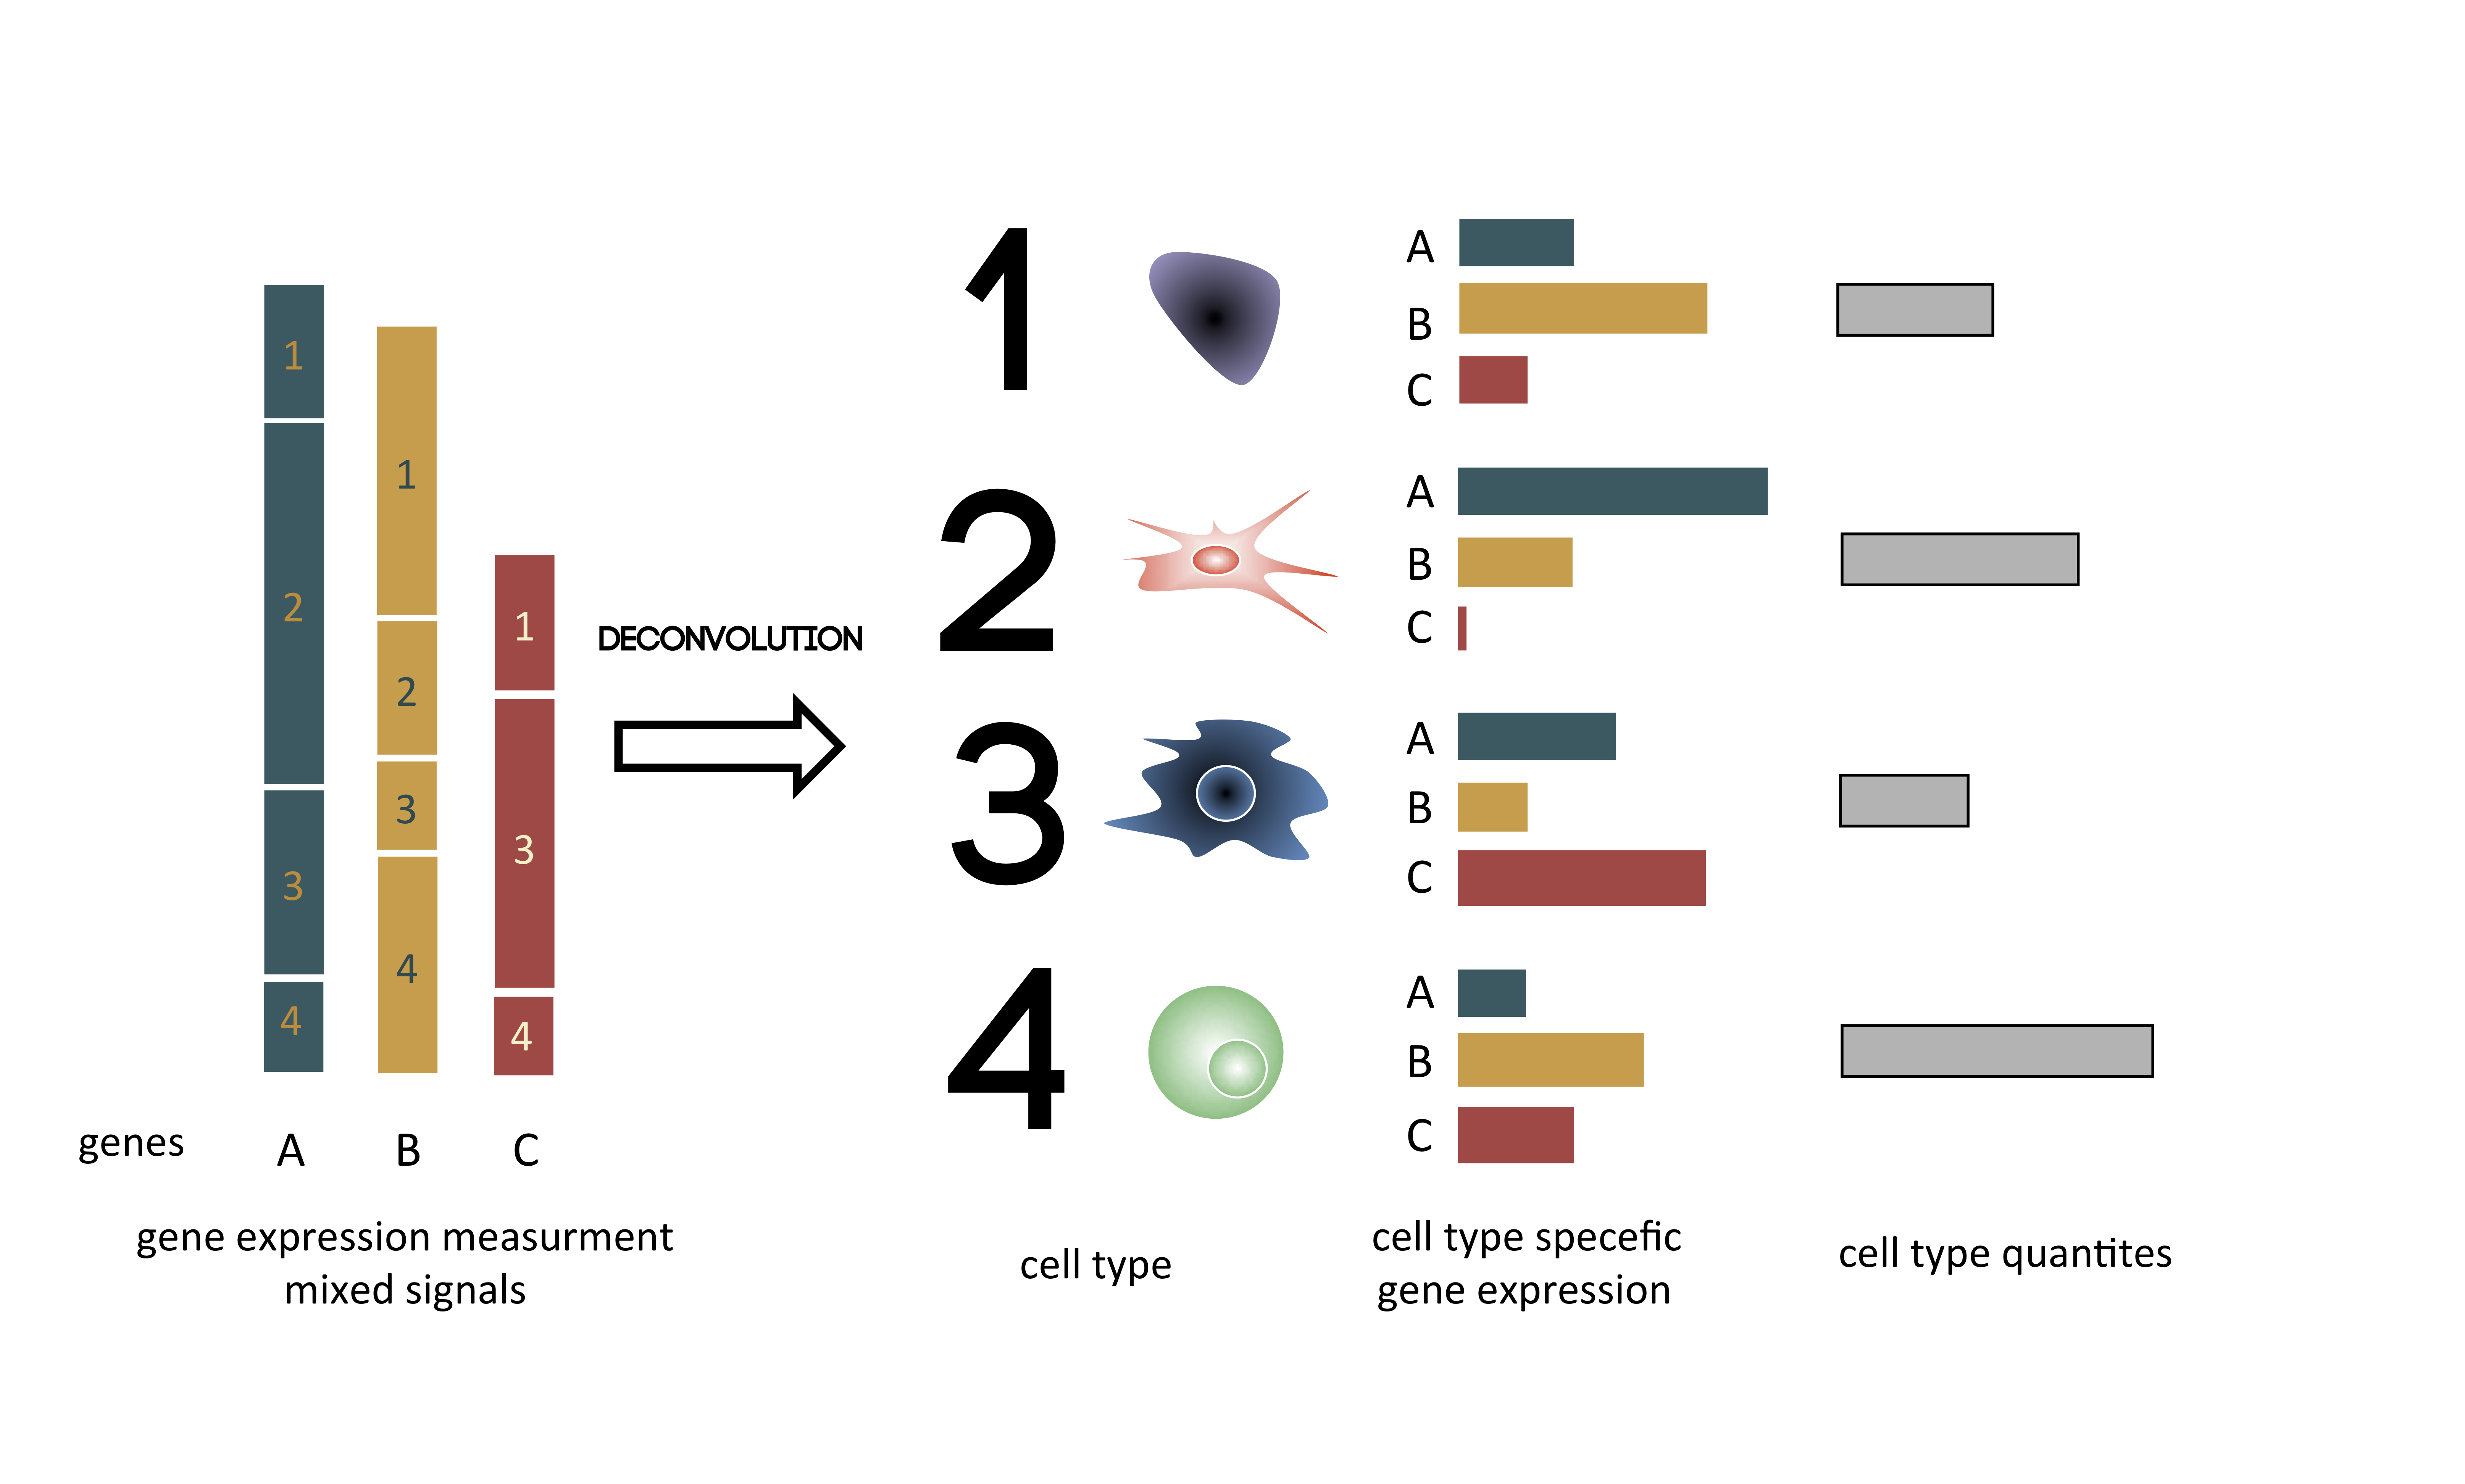
\includegraphics[width=1\linewidth]{figures-ext/deconv} 

}

\caption[Principle of the deconvolution applied to transcriptome]{\textbf{Principle of the
deconvolution applied to transcriptome} Graphical illustration of the
deconvolution of mixed samples. Starting from the left, gene expression
of genes A B C is a sum of expression of cell types 1, 2, 3, 4. After
deconvolution, cell types are separated, and gene expression of each
cell type is estimated taking into account cell type proportions.}\label{fig:deconvolution-cartoon}
\end{figure}








However, in this model, either the mixing proportions, number of mixing
sources or an array of specific genes need to be known. While, in the
real-life case, only \(X\) is truly known. Therefore, developed models
proposed various manners for estimating the number of mixing sources and
their proportions, or the specific cell type expression.

Why there is a need for cell-type deconvolution approaches?

\begin{itemize}
\tightlist
\item
  for differential gene expression analysis, to avoid confusion between
  a studied condition (i.e.~disease impact) and cell-type abundance
  (change in gene expression due to the change of cell proportions)
\item
  difference in gene expression in one cell type can be blurred by the
  presence of other cells expressing the gene
\item
  to obtain information about a fraction of given component in the
  sample
\item
  to study potential interactions between cell types in the studied
  context
\item
  to infer context-specific profile or signature
\end{itemize}

\hypertarget{literature-overview}{%
\subsection{Literature overview}\label{literature-overview}}

In order to answer general and specific need for cell-type deconvolution
of bulk transcriptomes researches produced a large collection of tools.
I have collected all (to my knowledge) articles published in journals or
as a pre-print (up to May 2018) that propose original models/tools of
\textbf{cell-type deconvolution of bulk transcriptomes} (Tab.
\ref{tab:mytab}). Therefore clonal deconvolution methods are not
included in this overview. The transcriptome-based purity estimation
methods are included as many of them proposed an initial 2-sources model
that could be, at least in theory, extended to multiple sources model.
Also, I did not include cell-type deconvolution methods of other data
types (such as methylome). A separate
\protect\hyperlink{otherDecon}{section 2.4} is dedicated to
non-transcriptome methods.

\#\#\#\#Growth of the field

The Table \ref{tab:mytab} contains 64 (including mine) deconvolution
methods. It can be observed (Fig. \ref{fig:pubyear}) that since the
begging of my thesis (2015) the number of publications has doubled (64
publications in 2018 vs.~33 in 2014). Also, from 2014 on, more methods
are published every year. In Fig. \ref{fig:pubyear} \emph{hallmark}
publications are indicated in red above their year of publication. The
three most popular methods (based on number of citations/number of years
since publication) are CIBERSORT \citep{Newman2015} (2015, total number
of citations: 343 and 88.75 citations per year), ESTIMATE
\citep{Yoshihara2013} (2013, total number of citations: 266 and 44.33
citations per year), and csSAM \citep{ShenOrr2010} (2010, total number
of citations: 286 and 31.77 citations per year). It can be noticed that
the high impact of the journal plays a role, the top 3 cited methods
were published in \emph{Nature Methods} and \emph{Nature Communications}
followed by Virtual Microdissection method \citep{Moffitt2015} (2015)
published in \emph{Nature Genetics}. However, the fifth most cited
publication \citet{Abbas2009} (2009, a total of 207 citations) appeared
in \emph{PLOS ONE}. As the index is a bit penalizing for recent
publications, among commonly cited tools after 2015 are MCPcounter with
42 citations (2016, 32 without self-citations) and xCell with 14
citations (2017, 11 without self-citations). A big number of
publications with a low number of citations were published in
\emph{Oxford Bioinformatics} or \emph{BMC Bioinformatics} which
underlines the importance of publishing a computational tool along with
an important biological message rather than in a technical journal in
order to increase a chance to be used by other researchers.

\hypertarget{availability}{%
\subsubsection{Availability}\label{availability}}

Another essential aspect is the availability of the tool. One-third (in
total 21) methods do not provide source code or a user-interface tool to
reproduce their results. Among those articles, 13 was published before
2015. Therefore, it can be concluded that the pressure of publishers and
research community on reproducibility and accessibility of bioinformatic
tools gives positive results. \citet{Shen-Orr2013}, authors of
semi-supervised NMF method \citep{Gaujoux2012}, published \emph{CellMIx:
a comprehensive toolbox for gene expression deconvolution} where he
implements most of previously published tools in R language and group
them in the same R-package. This work tremendously increased the
usability of previously published deconvolution methods. The CellMix
package is one of the state-of-the-art work on deconvolution that
regroups algorithms, signatures and benchmark datasets up to 2013.

\begin{landscape}\rowcolors{2}{gray!6}{white}
\begin{table}

\caption[Summary of methods for cell-type deconvolution of bulk transcriptome]{\label{tab:mytab}\textbf{Summary of methods for cell-type
deconvolution of bulk transcriptome}. Data gathered based on PubMed and
google scholar search in May 2018.}
\centering
\resizebox{\linewidth}{!}{
\begin{tabular}[t]{cccccccccccccc}
\hiderowcolors
\toprule
name & data & type & doi & year & application & availability & out.profiles & out.proportions & category & language & citations & pop.index & previously.covered\\
\midrule
\showrowcolors
GSVA scores & RNA-seq & supervised & https://doi.org/10.1158/1078-0432.CCR-17-3509 & 2018 & Cancer transcriptome & NA & FALSE & TRUE & enrichment & unknown & 1 & 1.00 & FALSE\\
MySort & MA & supervised & https://doi.org/10.1186/s12859-018-2069-6 & 2018 & Blood & https://testtoolshed.g2.bx.psu.edu/repository?repository\_id=6e9a9ab163e578e0\&changeset\_revision=e3afe097e80a & FALSE & TRUE & regression & R, web tool & 0 & 0.00 & FALSE\\
ADVOCATE & RNA-seq & supervised & https://doi.org/10.1101/288779 & 2018 & Cancer transcriptome & NA & TRUE & TRUE & probabilistic & R & 0 & 0.00 & FALSE\\
DTD & scRNA-seq & supervised & https://arxiv.org/abs/1801.08447v1 & 2018 & Cancer transcriptome & NA & FALSE & TRUE & regression & unknown & 0 & 0.00 & FALSE\\
CellDistinguisher & MA + RNA-seq & unsupervised & https://doi.org/10.1371/journal.pone.0193067 & 2018 & yeast cell cycle & https:// github.com/GeneralElectric/CcellDdistinguisher & TRUE & TRUE & convex hull & R & 0 & 0.00 & FALSE\\
\addlinespace
dtangle & MA + RNA-seq & supervised & https://doi.org/10.1101/290262 & 2018 & Blood & https://cran.r-project.org/package=dtangle & FALSE & TRUE & regression & R & 0 & 0.00 & FALSE\\
DeconICA & MA + RNA-seq & unsupervised & https://doi.org/10.5281/zenodo.1250069 & 2018 & Cancer transcriptome & https://urszulaczerwinska.github.io/DeconICA/ & TRUE & TRUE & matrix factorisation & R, matlab & 0 & 0.00 & FALSE\\
xCell & MA + RNA-seq & supervised & https://dx.doi.org/10.1186\%2Fs13059-017-1349-1 & 2017 & Cancer transcriptome & http://xcell.ucsf.edu/; https://github.com/dviraran/xCell & FALSE & TRUE & enrichment & R, web tool & 15 & 7.50 & FALSE\\
BioQC & MA + RNA-seq & supervised & https://doi.org/10.1186/s12864-017-3661-2 & 2017 & Gene expression & https://www.bioconductor.org/packages/release/bioc/html/BioQC.html & FALSE & FALSE & enrichment & R & 6 & 3.00 & TRUE\\
EPIC & RNA-seq & supervised & https://dx.doi.org/10.7554\%2FeLife.26476 & 2017 & Cancer transcriptome & https://github.com/GfellerLab/EPIC & FALSE & TRUE & regression & R & 4 & 2.00 & FALSE\\
\addlinespace
Estimation of immune cell content & scRNA-seq & supervised & https://doi.org/10.1038/s41467-017-02289-3 & 2017 & Cancer transcriptome & NA & FALSE & TRUE & regression & unknown & 3 & 1.50 & FALSE\\
Enumerateblood & MA & supervised & https://doi.org/10.1186/s12864-016-3460-1 & 2017 & Blood gene expression & https://github.com/cashoes/enumerateblood & TRUE & TRUE & probabilistic & R & 2 & 1.00 & TRUE\\
ImmunoStates & MA & supervised & https://doi.org/10.1101/206466 & 2017 & Blood, solid tissue, disease & NA & FALSE & TRUE & regression & R & 1 & 0.50 & FALSE\\
quanTIseq & RNA-seq + Images & supervised & https://doi.org/10.1101/223180 & 2017 & Cancer transcriptome & http://icbi.at/software/quantiseq/doc/index.html & FALSE & TRUE & regression & web tool & 1 & 0.50 & FALSE\\
SMC & MA & unsupervised & https://doi.org/10.1371/journal.pone.0186167 & 2017 & Tissue mixtures & https://github.com/moyanre/smcgenedeconv & TRUE & TRUE & probabilistic & matlab & 1 & 0.50 & FALSE\\
\addlinespace
Modular discrimination index & MA + RNA-seq & supervised & https://doi.org/10.1371/journal.pone.0169271 & 2017 & Skin tuberculosis & https://github.com/MJMurray1/MDIScoring & FALSE & TRUE & enrichment & R & 1 & 0.50 & FALSE\\
DemixT & MA + RNA-seq & supervised & https://doi.org/10.1101/146795 & 2017 & Cancer transcriptome & https://github.com/wwylab/DeMixT & TRUE & TRUE & probabilistic & R & 0 & 0.00 & FALSE\\
Post‐modified non‐negative matrix factorization & RNA-seq & unsupervised & https://doi.org/10.1002/cem.2929 & 2017 & Cancer transcriptome & NA & TRUE & TRUE & matrix factorisation & matlab & 0 & 0.00 & FALSE\\
Infino & RNA-seq & supervised & https://doi.org/10.1101/221671 & 2017 & Cancer transcriptome & https://github.com/hammerlab/infino & TRUE & TRUE & probabilistic & Stan & 0 & 0.00 & FALSE\\
MCPcounter & MA & supervised & https://doi.org/10.1186/s13059-016-1070-5 & 2016 & Cancer transcriptome & https://github.com/ebecht/MCPcounter & FALSE & TRUE & enrichment & R & 42 & 14.00 & TRUE\\
\addlinespace
ssGSEA applied to renal cell
carcinoma & RNA-seq & supervised & https://doi.org/10.1186/s13059-016-1092-z & 2016 & Cancer transcriptome & NA & FALSE & TRUE & enrichment & R & 40 & 13.33 & TRUE\\
CAM & MA & unsupervised & https://doi.org/10.1038/srep18909 & 2016 & yeast cell cycle & http://mloss.org/software/view/437, & TRUE & TRUE & convex hull & R-java & 12 & 4.00 & TRUE\\
Immune  Quant & undefined & supervised & https://doi.org/10.1093/bioinformatics/btw535 & 2016 & Human tissues & http://csgi.tau.ac.il/ImmQuant/ & FALSE & TRUE & regression & web tool & 5 & 1.67 & TRUE\\
VoCAL & MA, GWAS & supervised & https://doi.org/10.1371/journal.pcbi.1004856 & 2016 & Lung tissue & https://cran.r-project.org/web/packages/ComICS/index.html & FALSE & TRUE & regression & R & 5 & 1.67 & TRUE\\
CellMapper & MA & semi-supervised & https://doi.org/10.1186/s13059-016-1062-5 & 2016 & Brain tissue & http://bioconductor.org/packages/release/bioc/html/CellMapper.html & TRUE & FALSE & matrix factorisation & R & 5 & 1.67 & TRUE\\
\addlinespace
contamDE & RNA-seq & supervised & https://doi.org/10.1093/bioinformatics/btv657 & 2016 & Tumor purity & https://github.com/zhanghfd/contamDE/ & TRUE & TRUE & probabilistic & R & 4 & 1.33 & TRUE\\
ImSig & RNA-seq & supervised & https://doi.org/10.1101/077487 & 2016 & Cancer transcriptome & NA & FALSE & TRUE & enrichment & unknown & 0 & 0.00 & FALSE\\
CIBERSORT & MA & supervised & https://doi.org/10.1038/nmeth.3337 & 2015 & Cancer transcriptome & http://cibersort.stanford.edu/ & FALSE & TRUE & regression & R, web tool & 343 & 85.75 & TRUE\\
Virtual Microdissection & MA & unsupervised & https://doi.org/10.1038/ng.3398 & 2015 & detection of cancer and stroma in PDAC (TCGA) & NA & TRUE & TRUE & matrix factorisation & matlab & 86 & 21.50 & TRUE\\
CellCODE & MA & semi-supervised & https://doi.org/10.1093/bioinformatics/btv015 & 2015 & Blood & http://www.pitt.edu/\textasciitilde{}mchikina/CellCODE/ & TRUE & TRUE & matrix factorisation & R- C-C++- Fortran & 28 & 7.00 & TRUE\\
\addlinespace
CoD & RNA-seq & supervised & https://doi.org/10.1093/bioinformatics/btv498 & 2015 & Mice diseased tissues & http://www.csgi.tau.ac.il/CoD/ & FALSE & TRUE & regression & web tool & 4 & 1.00 & TRUE\\
DCQ & RNA-seq & supervised & https://dx.doi.org/10.1002\%2Fmsb.134947 & 2014 & Mice blood under flu infection & http://www.dcq.tau.ac.il/ & FALSE & TRUE & regression & web tool & 32 & 6.40 & TRUE\\
UNDO & MA & unsupervised & https://doi.org/10.1093/bioinformatics/btu607 & 2014 & Cancer transcriptome & https://www.bioconductor.org/packages/release/bioc/html/UNDO.html & TRUE & TRUE & matrix factorisation & R & 18 & 3.60 & TRUE\\
ESTIMATE & MA + RNA-seq & supervised & https://doi.org/10.1038/ncomms3612 & 2013 & Cancer transcriptome & https://sourceforge.net/projects/estimateproject/ & FALSE & TRUE & enrichment & R & 266 & 44.33 & TRUE\\
DeconRNASeq & RNA-seq & supervised & https://doi.org/10.1093/bioinformatics/btt090 & 2013 & Tissue mixtures & https://www.bioconductor.org/packages/release/bioc/html/DeconRNASeq.html & FALSE & TRUE & regression & R & 52 & 8.67 & TRUE\\
\addlinespace
DSA & MA & supervised & https://dx.doi.org/10.1186\%2F1471-2105-14-89 & 2013 & Cancer transcriptome & https://github.com/zhandong/DSA & TRUE & TRUE & regression & R & 52 & 8.67 & TRUE\\
ISOpure & MA & supervised & https://doi.org/10.1186/gm433 & 2013 & Cancer transcriptome & https://qlab.faculty.ucdavis.edu/isopure/ & TRUE & TRUE & probabilistic & matlab, R & 44 & 7.33 & TRUE\\
DeMix & MA & supervised & https://doi.org/10.1093/bioinformatics/btt301 & 2013 & Cancer purity & http://odin.mdacc.tmc.edu/∼wwang7/DeMix.html. & TRUE & TRUE & probabilistic & C, R & 38 & 6.33 & TRUE\\
Nanodissection & MA & supervised & https://doi.org/10.1101/gr.155697.113 & 2013 & Chronic kidney disease (Cell lineages) & http://nano.princeton.edu/ & FALSE & TRUE & regression & web tool & 33 & 5.50 & TRUE\\
TIMER & MA + RNA-seq & supervised & https://doi.org/10.1186/s13059-016-1028-7 & 2013 & Cancer transcriptome & http://cistrome.org/TIMER/ & FALSE & TRUE & regression & web tool & 33 & 5.50 & TRUE\\
\addlinespace
Self-directed Method for Cell-Type Identification & MA & unsupervised & https://doi.org/10.1371/journal.pcbi.1003189 & 2013 & Cancer transcriptome & NA & TRUE & TRUE & matrix factorisation & matlab & 18 & 3.00 & TRUE\\
MMAD & MA & BOTH & https://doi.org/10.1093/bioinformatics/btt566 & 2013 & in vitro tissue mlxtures & http://sourceforge.net/projects/mmad/ & TRUE & TRUE & regression & matlab & 11 & 1.83 & TRUE\\
Statical mechanics approach & undefined & unsupervised & https://arxiv.org/abs/1210.7508v1 & 2013 & Udefined & NA & TRUE & TRUE & probabilistic & unknown & 2 & 0.33 & FALSE\\
TEMT & RNAseq & supervised & https://bmcbioinformatics.biomedcentral.com/articles/10.1186/1471-2105-14-S5-S11 & 2013 & in vitro cell mixtures & https://github.com/uci-cbcl/TEMT & FALSE & TRUE & probabilistic & python & 0 & 0.00 & TRUE\\
Semi-supervised Nonnegative Matrix Factorization & MA & semi-supervised & https://doi.org/10.1016/j.meegid.2011.08.014 & 2012 & Blood & https://web.cbio.uct.ac.za/\textasciitilde{}renaud/CRAN/web/CellMix/ & TRUE & TRUE & matrix factorisation & R & 61 & 8.71 & TRUE\\
\addlinespace
PERT & MA & supervised & https://doi.org/10.1371/journal.pcbi.1002838 & 2012 & blood & https://github.com/gquon/PERT & TRUE & TRUE & probabilistic & octave & 33 & 4.71 & TRUE\\
CTen & MA & supervised & https://doi.org/10.1186/1471-2164-13-460 & 2012 & Infected lung tissue & http://www.influenza-x.org/\textasciitilde{}jshoemaker/cten/ & TRUE & FALSE & enrichment & web tool & 31 & 4.43 & TRUE\\
PSEA & MA & supervised & https://doi.org/10.1038/nmeth.1710 & 2011 & Brain tissue & https://bioconductor.org/packages/release/bioc/html/PSEA.html & FALSE & TRUE & regression & R & 96 & 12.00 & TRUE\\
Quadratic programming & MA & supervised & https://doi.org/10.1371/journal.pone.0027156 & 2011 & Blood & NA & FALSE & TRUE & regression & unknown & 76 & 9.50 & TRUE\\
SPEC & MA & supervised & https://doi.org/10.1186/1471-2105-12-258 & 2011 & Blood & http://clip.med.yale.edu/SPEC/ & FALSE & TRUE & enrichment & R & 39 & 4.88 & TRUE\\
\addlinespace
csSAM & MA & supervised & https://doi.org/10.1038/nmeth.1439 & 2010 & Blood & https://github.com/shenorrLab/csSAM & TRUE & FALSE & regression & R & 286 & 31.78 & TRUE\\
Statistical expression deconvolution & MA & supervised & https://doi.org/10.1093/bioinformatics/btq097 & 2010 & Cancer xenografts & NA & FALSE & TRUE & regression & unknown & 53 & 5.89 & TRUE\\
DSection & MA & supervised & https://doi.org/10.1093/bioinformatics/btq406 & 2010 & Tissue mixtures & http://informatics.systemsbiology.net/DSection & TRUE & FALSE & probabilistic & matlab & 52 & 5.78 & TRUE\\
deconf & MA & unsupervised & https://doi.org/10.1186/1471-2105-11-27 & 2010 & Blood & https://static-content.springer.com/esm/art\%3A10.1186\%2F1471-2105-11-27/MediaObjects/12859\_2009\_3484\_MOESM1\_ESM.ZIP & TRUE & TRUE & matrix factorisation & R & 41 & 4.56 & TRUE\\
Abbas regression & MA & supervised & https://doi.org/10.1371/journal.pone.0006098 & 2009 & Blood & NA & FALSE & TRUE & regression & R & 207 & 20.70 & TRUE\\
\addlinespace
ISOLATE & MA & supervised & https://dx.doi.org/10.1093\%2Fbioinformatics\%2Fbtp378 & 2009 & Cancer transcriptome & https://qlab.faculty.ucdavis.edu/isolate/ & TRUE & TRUE & matrix factorisation & matlab & 37 & 3.70 & TRUE\\
Electronical substraction & MA & supervised & https://doi.org/10.1093/bioinformatics/btm508 & 2007 & Infected macrophages & NA & TRUE & TRUE & regression & unknown & 30 & 2.50 & TRUE\\
Computational expression deconvolution & MA & supervised & https://doi.org/10.1186/1471-2105-7-328 & 2006 & Murine mammary gland & NA & FALSE & TRUE & regression & unknown & 36 & 2.77 & TRUE\\
Robust Computational Reconstitution & MA & supervised & https://doi.org/10.1186/1471-2105-7-369 & 2006 & Synovial tissue (cell types in silico) & NA & FALSE & TRUE & regression & unknown & 6 & 0.46 & TRUE\\
MHMM & MA & unsupervised & https://doi.org/10.1089/cmb.2006.13.1749 & 2006 & Yeast cell cycle & NA & TRUE & TRUE & probabilistic & unknown & 4 & 0.31 & TRUE\\
\addlinespace
In silico microdissection & MA & unsupervised & https://doi.org/10.1186/1471-2105-6-54 & 2005 & In vitro tissue mixtures & NA & TRUE & TRUE & probabilistic & unknown & 45 & 3.21 & TRUE\\
Mixture models & MA & supervised & https://doi.org/10.1093/bioinformatics/bth139 & 2004 & Cancer transcriptome & broken link & TRUE & TRUE & probabilistic & R & 66 & 4.40 & TRUE\\
DECONVOLUTE & MA & supervised & https://doi.org/10.1073/pnas.1832361100 & 2003 & yeast cell cycle & broken link & FALSE & TRUE & regression & Java 2 & 135 & 8.44 & TRUE\\
Direct method & MA & unsupervised & https://www.ncbi.nlm.nih.gov/pubmed/11473019 & 2001 & cander and normal tissue & NA & TRUE & TRUE & matrix factorisation & unknown & 96 & 5.33 & TRUE\\
\bottomrule
\end{tabular}}
\end{table}
\rowcolors{2}{white}{white}
\end{landscape}





The most popular language of implementation of published methods is R
(49.2 \%), followed by Matlab (11.11\%), only one tool so far was
published in Python.

\hypertarget{data-type}{%
\subsubsection{Data type}\label{data-type}}

Also, most of the methods were designed to work with microarray data.
There is a high chance that some of them are adaptable to RNA-seq.
However, a little number of older methods was tested in a different
setup. For some method, as CIBERSORT, demonstrated to work with
microarray and applied commonly to RNA-seq by other researchers, the
validity of results remains unclear as some studies claim that CIBERSORT
performs accurately applied to RNA-seq \citep{Thorsson2018} and other
opt against it \citep{Li2017, Tamborero2018}. Most of newer methods
(i.e.~EPIC \citep{Racle2017}, quanTIseq \citep{Finotello2017} or Infino
\citep{Zaslavsky2017}) are specifically designed for RNA-seq
TPM-normalized data. Some methods, mostly enrichment-based methods, are
applicable to both technologies (i.e.~xCell \citep{Aran2017}).

\hypertarget{objectives-of-the-cell-type-deconvolution}{%
\subsubsection{Objectives of the cell-type
deconvolution}\label{objectives-of-the-cell-type-deconvolution}}

It is remarkable that the general aim of the cell-type deconvolution
changed with time. The earlier methods aimed to improve the power of
differential expression analysis though \emph{purification} of the gene
expression. For example, to compare differentially expressed genes (DEG)
in T-cell from the blood under two conditions. However, the obtained
purified profiles from complex mixtures were often uncertain
\citep{Onuchic2016}. Recently, the most mentioned goal of deconvolution
is a quantification of proportions of different cell types, especially
in the context of cancer transcriptomes motivated by redefinition of
immunophenotypes discussed in the previous chapter. The most popular
tissue of interest for deconvolution algorithms are cancer tissues and
blood. Other applications are cell-cycle time-dependent fluctuations of
yeast, brain cells, and glands .

\hypertarget{differences-between-approaches}{%
\subsubsection{Differences between
approaches}\label{differences-between-approaches}}

Mathematically speaking, I have divided methods into four categories:
probabilistic, regression, matrix factorisation and convex hull
depending on the nature of the approach. Most of the methods (48 -
74.6\%) are working within a supervised framework, and only 20\% (14)
are unsupervised. The approaches will be described in detail in the
following section.

There are numerous practical differences between the methods.
\citet{Shen-Orr2013} in their review of deconvolution tools grouped the
tools depending on their inputs and outputs. Given the type of outputs,
deconvolution can be considered as complete (proportions and cell
profiles) or partial (one of those). Moreover, the inputs of the
algorithms can be important to evaluate how practical the tool is. The
most popular tools and the most recent tools ask for minimal input from
the user: the bulk gene expression matrix, or even raw sequencing data
\citep{Finotello2017}. Older methods usually request either at least
approximative proportions of mixed cells or purified profiles to be
provided. The newer methods include the reference profiles in the tool
if necessary. Some tools, including most of purity estimation tools,
demand an additional data input as normal samples or another data type
such as CNA data (Timer \citep{Li2013}, VoCAL \citep{Steuerman2016}) or
image data (quanTIseq \citep{Finotello2017}). An important parameter is
also a number of sources (\(k\)) to which the algorithm deconvolutes the
mixture. In many methods, it should be provided by the user, which can
be difficult in a case of complex mixtures of human tissues. Besides,
type of method can also limit the number of sources, for example, a
probabilistic framework privilege lower number of sources (2-3) due to
the theoretical constraints. In regression depending on provided
reference the output number of estimated sources is imposed. Because of
the problem of collinearity and similarity of immune cell profiles, it
is hard to distinguish between cell sub-types, deconvolution into
fine-grain cell subtypes is often called often deep deconvolution. Some
methods (i.e., CIBERSORT, Infino, xCell) give specific attention to
deconvolution of cell-subtypes. An absolute presence of a cell type in
the mixture can also be an essential factor. If it is too low it can
reach a detection limit, Electronic subtraction \citep{Gosink2007}
discuss specifically the detection of rare cel-types.

\hypertarget{computational-efficiency}{%
\subsubsection{Computational
efficiency}\label{computational-efficiency}}

Running time and the necessary infrastructure are another way to
characterize the methods. Although it is hard to compare the running
time objectively simultaneously of all the tools because of the
heterogeneity of methods and different datasets analysed, some
tendencies can be observed. If one thinks about applying deconvolution
methods to big cohorts, regression and enrichment-based methods should
be well suited. As far as matrix factorisation is concerned, it depends
on the implementation (i.e.~R vs Matlab) and if the number of sources
needs to be estimated (multiple runs for different \(k\) parameter) or
if a stabilisation needs to applied (multiple runs for the same \(k\)
parameter). Finally, probabilistic tools seem to be challenging to
scale, i.e.~authors of Infino admit that their pipeline is not yet
applicable at high-throughput.

In order to let user better understand the differences between different
mathematical approaches, I will introduce shortly the types of
approaches used for cell-type deconvolution of transcriptomes as well as
their strong and weak points.

\begin{figure}

{\centering 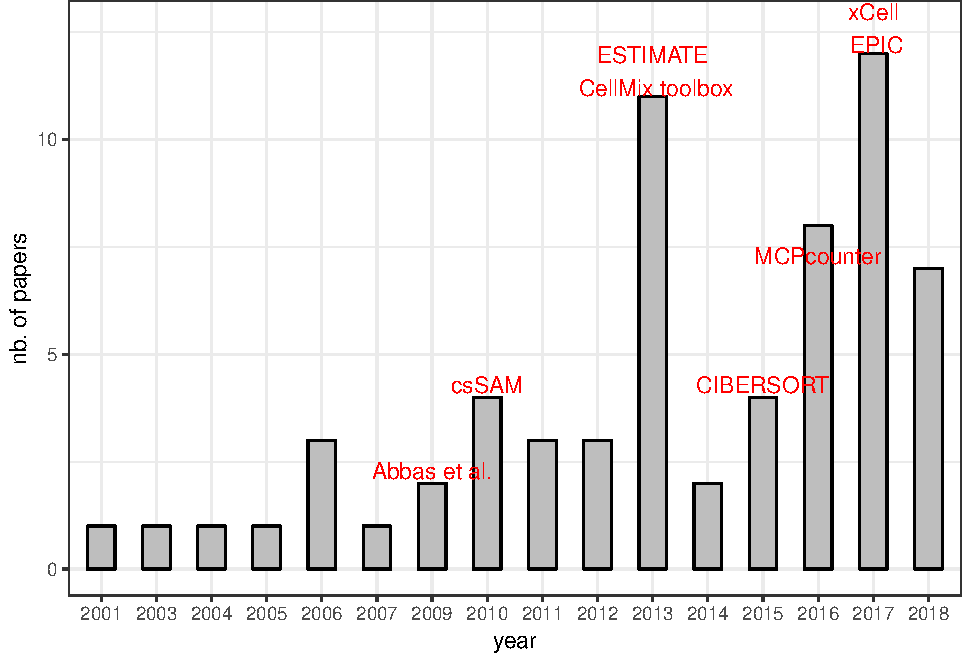
\includegraphics[width=0.7\linewidth]{UCzPhDThesis_files/figure-latex/pubyear-1} 

}

\caption[Distribution of publications of cell-type deconvolution of bulk transcriptome over the years]{\textbf{Distribution of publications of cell-type
deconvolution of bulk transcriptome over the years}. In red: hallmark
publications. Data gathered based on PubMed and google scholar search in
May 2018.}\label{fig:pubyear}
\end{figure}






\begin{figure}
\subfloat[approach type\label{fig:languages1}]{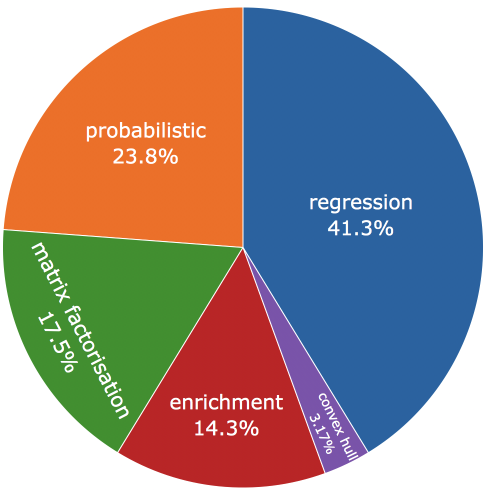
\includegraphics[width=0.33\linewidth]{./figures-ext/piechartA} }\subfloat[supervised/unsupervised\label{fig:languages2}]{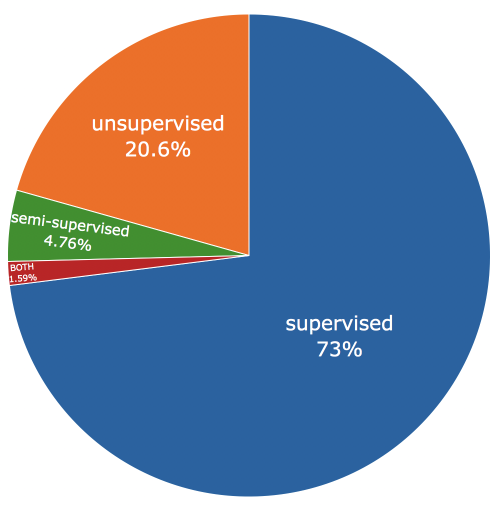
\includegraphics[width=0.33\linewidth]{./figures-ext/pichartB} }\subfloat[programming language\label{fig:languages3}]{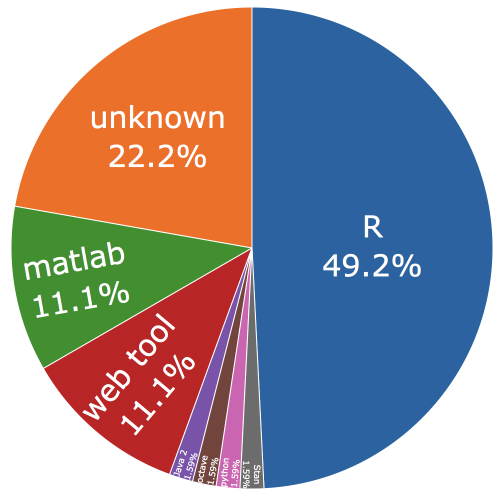
\includegraphics[width=0.33\linewidth]{./figures-ext/pirChart} }\caption[Simple statistics illustrating characteristics of published cell-type deconvolution tools]{\textbf{Simple statistics illustrating
characteristics of published cell-type deconvolution tools}:
\ref{fig:languages1} - Percentage of used approach type,
\ref{fig:languages2} - Percentage of supervised/unsupervised tools,
\ref{fig:languages3} - Percentage of the programming languages of
implementation. Data gathered based on pubmed and google scholar search
in May 2018.}\label{fig:languages}
\end{figure}









\hypertarget{regression-based-methods}{%
\subsection{Regression-based methods}\label{regression-based-methods}}

Regression models are the most popular methods for bulk gene expression
deconvolution. They use estimated pure cell profiles as depending
variables (or selected signature genes) that should explain the mixed
profiles choosing best \(\beta\) parameters (Eq. \eqref{eq:regLin}) that
can be interpreted as cell proportions.

A standard type of regression is called linear regression. It reflects
linear dependence between independent and dependent variables. The
linear regression was developed in the \emph{precomputer age of
statistics} \citep{Hastie2009}.

In linear regression, we want to predict a real-valued output \(Y\),
given a vector \(X^T = (X_1,X_2,… ,X_p)\). The linear regression model
has the form:

\begin{equation}
f(X) = \beta_0 + \sum_{j=1}^{p} X_j\beta_j \label{eq:regLin}
\end{equation}

Where the \(\beta_j\)s are unknown parameters or coefficients, and
\(X_j\)s are the explaining variables. Given pairs of
(\(x_1\),\(y_1\))\ldots{}(\(x_N\) ,\(y_N\) ), one can estimate
coefficients \(\beta\) with an optimization of an objective function
(also called cost function).

The most popular estimation method is \textbf{least squares}, the
coefficients \(\beta = (\beta_0, \beta_1, ..., \beta_n)\) are computed
to minimize the residual sum of squares (RSS):

\begin{equation}
RSS(\beta) = \sum_{i = 1}^{N}(y_i - f(x_i))^2 = \sum_{i = 1}^{N}(y_i - \beta_0 - \sum_{j=1}^p x_i\beta_j)^2 \label{eq:rss}
\end{equation}

\textbf{Ordinary least squares regression} is using Eq.\eqref{eq:rss} to
compute \(\beta\).

\textbf{Ridge regression} (Eq.\eqref{eq:ridge}) (aka Tikhonov
regularization) adds a regularizer (called \(L2\) norm) to shrink the
coefficients (\(\lambda \geq 1\)) through imposing a penalty on their
size.

\begin{equation}
\hat{\beta}^{ridge} = \underset{\beta}{\text{argmin}}\{\sum_{i = 1}^{N}(y_i - f(x_i))^2 + \lambda\sum_{j=1}^{p}\beta^2_j\}\label{eq:ridge}
\end{equation}

Similarly \textbf{Lasso regression} (Equation \eqref{eq:lasso}) adds a
regularization term to RSS (called \(L1\) norm), it may set coefficients
to 0 and therefore perform feature selection.

\begin{equation}
\hat{\beta}^{ridge} = \underset{\beta}{\text{argmin}}\{\sum_{i = 1}^{N}(y_i - f(x_i))^2 + \lambda\sum_{j=1}^{p}\lvert\beta_j\rvert\}\label{eq:lasso}
\end{equation}

In \textbf{Elastic net regression} both penalties are applied.

\textbf{Support Vector Regression (SVR)} is regression using
\textbf{Supported Vector Machines (SVM)}. In SVR \(\beta\) can be
estimated as follows:

\begin{equation}
H(\beta,\beta_0) = \sum_{i=1}^{N} V (y_i − f(x_i)) +\frac{λ}2\lVert\beta\rVert^2 \label{eq:svr1}
\end{equation}

where error is measured as follows:

\begin{equation}
V_\epsilon(r) = \begin{cases}
    0, & \text{if $\lvert r \rvert < \epsilon$,}\\
    \rvert r\lvert - \epsilon, & \text{otherwise}.
  \end{cases}  \label{eq:svr2}
\end{equation}

with \(\epsilon\) being the limit of error measure, meaning errors of
size less than \(\epsilon\) are ignored.

In the SVM vocabulary, a subset of the input data that determine
hyperplane boundaries are called the \textbf{support vectors}
(Fig.\ref{fig:svr}). SVR discovers a hyperplane that fits the maximal
possible number of points within a constant distance, \(\epsilon\), thus
performing a regression.

In brief, in SVR, RSS is replaced by a linear \(\epsilon\)-insensitive
loss function and uses \emph{L}2-norm penalty function. There exist
variants of SVR algorithm, i.e. \(\epsilon\)-SVR \citep{drucker1997} and
\(\nu\)-SVR \citep{Scholkopf2000}. \(\epsilon\)-SVR allows to control
the error; this favors more complex models. In the \(\nu\)-SVR the
distance of the \(\epsilon\) margin can be controlled and therefore the
number of data points used for regression can be controlled.
\citet{Ju2013} used an SVM-based method to define cell type-specific
genes. A model using \(\nu\)-SVR with linear kernel was used by
\citet{Newman2015} in CIBERSORT.

\begin{figure}

{\centering 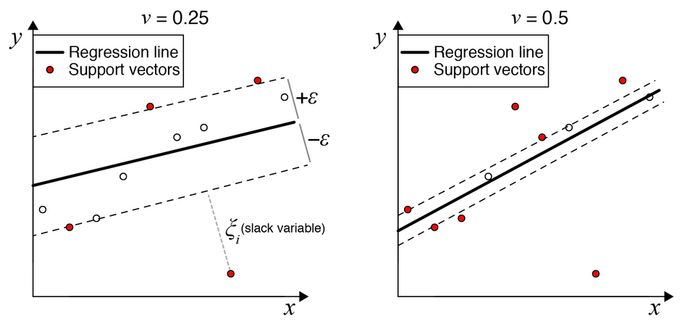
\includegraphics[width=1\linewidth]{figures-ext/vSVR} 

}

\caption[Priciple of the SVR regression]{\textbf{Principle of the SVR regression}. In SVR
regression \(\epsilon\) represents the limit of error measure, input
data points higher than \(+\epsilon\) or lower than \(-\epsilon\) are
called support vectors. The \(\nu\) parameter in \(\nu\)-SVR regression
controls the distance of training error bonds: left - lower \(\nu\)
value larger bound, right - higher \(v\) margin, smaller bound.
Reprinted by permission from Springer Nature \citep{Newman2015} © 2018
Macmillan Publishers Limited, part of Springer Nature. All rights
reserved.}\label{fig:svr}
\end{figure}











As unconstrained optimization of the objective function can result in
negative coefficients, in the context of cell-type deconvolution,
authors often aim to avoid as it complicates the interpretation.
Therefore, different constraints can be imposed on the \(\beta\)
coefficients. The most common conditions are
\(\beta_0 +\beta_1+ ...+\beta_n =1\) and \(\forall\beta_i \geq 0\).
Solution respecting the non-negativity condition is also called
non-negative least squares (NNLS) to contrast with ordinary least
squares (OLS). NNLS was adopted by many authors
\citep{Venet2001, Abbas2009, Repsilber2010, Zuckerman2013, Wang2016}.

The task can also be solved differently from the computational
perspective. \citet{Lu2003} and \citet{Wang2006} propose to use
simulated annealing to minimize the cost function. \citet{Gong2011}
proposed to solve the task using quadratic programming.

An extensive review on optimization of the objective function for
regression methods in cell-type deconvolution was published by
\citet{Mohammadi2017}. Authors carefully consider different
possibilities of parameter choice in the loss and regularization
formulations and its performance. They present as well recommendations
for construction of basis matrix and data pre- and post-processing.
Digital tissue deconvolution (DTD) \citep{Gortler2018} aims to train the
loss function with \emph{in silico} mixtures of single cell profiles
resulting in improved performance of rare cell types (present in a small
proportion). However, the training is computationally heavy, and the
proper training data for bulk transcriptomes are not available.

Since the publication of CIBERSORT \citep{Newman2015} some authors
\citep{Chen2018, Schelker2017} used the \citet{Newman2015}
implementation directly with pre/post modifications or with different
basis matrix or they re-implemented the SVR regression in their tools
\citep{Chen2018}.

Another recent method EPIC \citep{Racle2017} introduced weights related
to gene variability. In their constrained regression, they add it
explicitly in the cost function modifying RSS (Eq.\eqref{eq:rss}):

\begin{equation}
RSS^{weighted} (\beta) = \sum_{i = 1}^{N}(y_i - \beta_0 - w_i \sum_{j=1}^p x_i\beta_j)^2  \label{eq:epic}
\end{equation}

with the non-negativity and the sum constraints, we discussed above. The
\(w_i\) weights are corresponding to the variance of the given gene
measure in the same cell type. It aims to give less importance to the
genes variant between different measurements of the same cell-type. EPIC
also allows a cell type that is not a referenced in the signature matrix
with an assumption that the non-referenced cell type is equal to 1- a
sum of proportions of other cell types (Eq.\eqref{eq:tumorcoeff}). Authors
interpret this non-referenced cell type as the tumor fraction:

\begin{equation}
\beta_m = 1 - \sum_{j=1}^{m-1}\beta_j \label{eq:tumorcoeff}
\end{equation}

An additional feature of EPIC is advanced data normalization and
estimation of mRNA produced by each cell to adjust cell proportions,
which was previously proposed by \citet{Liebner2014} in the context of
microarray data:

\begin{equation}
p_j=\alpha \frac{\beta_j}{r_j} \label{eq:norm}
\end{equation}

where \(p_j\) are actual cell proportions that are `normalized' with
empirically derived coefficient \(\alpha\) and measured \(r_j\) is the
number of RNA nucleotides in cell type~\(j\).

Recently CIBERSORT proposed an \emph{absolute mode} where the
proportions are not relative to the leucocyte infiltration but to the
sample. It can be obtained with an assumption that the estimation of the
proportion of all genes in CIBERSORT matrix is corresponding to sample
purity. This functionality was not yet officially published, and it is
still in experimental phase \citep{Newman}.

Regression methods combined with pre- and post-processing of data can
result in estimation of proportions that can be interpreted directly as
a percentage of cells in a mixed sample. It is an important feature hard
to achieve with other methods. Some methods provide relative proportions
of the immune infiltrate \citep{Newman2015} and another aim to provide
absolute abundance \citep{Racle2017}. The absolute proportions are
easily comparable between data sets and cell types. Regression-based
methods are usually quite fast and can process large transcriptomic
cohorts. However, as I will discuss in
\protect\hyperlink{Validation}{Validation} section, they pose on the
hypothesis that the reference profiles available in some context (i.e.,
blood) are valid in a different one (i.e., tumor) or that profiles
extracted from one data type (scRNA-seq) are adapted to deconvolute bulk
RNAseq. Most of the recent regression methods focused on estimating
proportions and do not estimate context-specific profiles and can
process as little as one sample.

\hypertarget{enrichment-based-methods}{%
\subsection{Enrichment-based methods}\label{enrichment-based-methods}}

\rowcolors{2}{gray!6}{white}\begin{table}

\caption[Contangency table]{\label{tab:contangency}\textbf{Contingency table} is the count of overlap of
genes present in a certain condition (Y) vs.~not present (Y-Z) and
association to a pathway X (in X or not in X). The contingency table is
used in the frequency based test as Fisher exact test.}
\centering
\begin{tabular}[t]{|>{}l|>{}c|c}
\hiderowcolors
\toprule
\rowcolor{Gray}  \textcolor{white}{\textbf{ }} & \textcolor{white}{\textbf{Y}} & \textcolor{white}{\textbf{Z-Y}}\\
\midrule
\showrowcolors
in X & a & b\\
not in X & c & d\\
\bottomrule
\end{tabular}
\end{table}\rowcolors{2}{white}{white}






Enrichment-based methods aim to evaluate an amount of activity of a
given list of genes within the data. This can be obtained by calculating
a score based on gene expression. Traditionally enrichment methods were
used to analyze set of DEG. Different statistical approaches were
adapted: like Fisher exact test giving a p-value that estimated the
chance a given list of genes is over/under present in the input list of
DEGs and therefore characterize the condition vs.~control expressed
genes.

Let's take an example; if one wants to compute enrichment in pathway X
of the list of DEG genes Y with the total number of tested genes Z, a
contingency table need to be constructed (Tab. \ref{tab:contangency}).

In the Fisher exact test formula (Eq. \eqref{eq:fisher}) the \(a\),
\(b\),\(c\) and \(d\) are the individual frequencies, i.e.~number of
genes in of the 2X2 contingency table, and \(N\) is the total frequency
(\(a + b + c + d\)).

\begin{equation}
p= \frac{( ( a + b ) ! ( c + d ) ! ( a + c ) ! ( b + d ) ! )}{a ! b ! c ! d ! N ! } \label{eq:fisher}
\end{equation}

Another important (\textgreater{}14000 citations) algorithm computing
such a score (enrichment score ES) is named gene set enrichment analysis
(GSEA) \citep{Subramanian2005} uses sum-statistics. The list of genes
user wants to test for enrichment is usually ranked by fold change odd
or p-value of DGE analysis.

The high score indicated high activity of genes included in the list.
GSEA can also indicate an anti-activity of correlation. A variant of
GSEA, single sample GSEA (ssGSEA) \citep{Barbie2009} was used by
\citet{Senbabaoglu2016}, \citet{Yoshihara2013} and \citet{Aran2017} to
compute infiltration scores. In the ssGSEA genes are ranked by their
absolute expression. A variance-based variant of GSEA - GSVA
\citep{Hanzelmann2013} was used by \citet{Tamborero2018} for the same
purpose. MCPcounter \citep{Becht2016} uses an arithmetic mean of gene
expression of highly specific signature genes to compute a score.

In this way obtained scores, are not comparable between different cell
types and datasets. Therefore some authors propose normalization
procedures that make the score more comparable. For instance, xCell uses
a platform-specific transformation of enrichment scores. Similarly,
Estimate transforms scores for TCGA though an empirically derived
formula. MCPcounter authors use z-scoring to minimize platform-related
differences. Unfortunately, the normalization is not directly included
in the R package

Even though enrichment methods do not try to fit the linear model and
derived scores are not mathematically conditioned to represent cell
proportions; usually there can be observed a strong linear dependence.
An advantage of the enrichment-based methods is the speed and
possibility to include distinct signatures that can characterize
cell-types and cell-states of different pathways.

\hypertarget{probabilistic-methods}{%
\subsection{Probabilistic methods}\label{probabilistic-methods}}

The probabilistic methods share a common denominator: they aim to
minimise a likelihood function of Bayes' theorem:

\begin{equation}
p(y|\theta) = \frac{p(\theta|y )* p(y)}{p(\theta)} \label{eq:Bayes}
\end{equation}

In Eq.\eqref{eq:Bayes} \(y\) is our data, \(\theta\) a parameter,
\(p(y|\theta)\) \emph{posterior}, \(p(\theta|y )\) \emph{likelihood} and
\(p(\theta)\) \emph{prior}. Prior distribution is what we know about the
data before it was generated and combined with a probability
distribution of the observed data is called posterior distribution. The
likelihood describes how likely it is to observe the data (\(y\)) given
the parameter \(\theta\) (probability of \(y\) given \(\theta\) -
\(p(y|\theta)\)). A parameter is characteristic of a chosen model and a
hyperparameter is a parameter of prior distribution.

In the literature, there are mainly different types of probabilistic
models, one that assumes some type of distribution of mixed sources
(i.e., Gaussian or Poisson), others that learn the distribution
parameters empirically from a training set, another that try to find the
parameters of the distribution given the number of given sources. Then
in each case, there are different ways of constructing different priors
and posteriors functions. Among used techniques are Markov Chain Monte
Carlo or Expectation-Maximisation, which themselves can be implemented
in different ways
\citep[\citet{Zaslavsky2017}]{Erkkila2010, Ghosh2004, Lahdesmaki2005, Li2013, Roy2006}.

The probabilistic approaches are the most popular for purity estimation
(2 components models), that seems to be possible to extend to
3-components model \citep{Wang2017}. As far as cell-type decomposition
into a number of cells is concerned, a method published on BioRxiv
\emph{Infino} uses Bayesian inference with a generative model, trained
on cell type pure profiles. Authors claim their method is notably suited
for deep deconvolution that is able to build cell type similarities and
estimate the confidence of the estimated proportions which help to
interpret the results better.

A probabilistic framework is an attractive approach with solid
statistical bases. It can be suited to many specific cases. The pitfalls
are (1) the need of prior profiles or correct hypothesis on the
distribution parameters (2) reduced performance when applied to high
dimensional datasets due to extensive parameters search.

\hypertarget{convex-hull-based-methods}{%
\subsection{Convex-hull based methods}\label{convex-hull-based-methods}}

An emerging family of BSS methods is convex geometry (CG)-based methods.
Here, the \emph{sources} are found by searching the facets of the convex
hull spanned by the mapped observations solving a classical convex
optimization problem \citep{Yang2015}. It can be implemented in many
ways \citep{Preparata1985}.

\textbf{Convex hull} can be defined as follows \citep{Erickson2018}:

\begin{quote}
\emph{We are given a set \(P\) of \(n\) points in the plane. We want to
compute something called the \textbf{convex hull} of \(P\). Intuitively,
the convex hull is what you get by driving a nail into the plane at each
point and then wrapping a piece of string around the nails. More
formally, the convex hull is the smallest convex polygon containing the
points:}
\end{quote}

\begin{quote}
\begin{itemize}
\item
  \emph{\textbf{polygon}}: \emph{A region of the plane bounded by a
  cycle of line segments, called \textbf{edges}, joined end-to-end in a
  cycle. Points, where two successive edges meet, are called
  \textbf{vertices}.}
\item
  \emph{\textbf{convex}: For any two points \(p\), \(q\) inside the
  polygon, the line segment \(pq\) is completely inside the polygon.}
\item
  \emph{\textbf{smallest}}: \emph{Any convex proper subset of the convex
  hull excludes at least one point in \(P\). This implies that every
  vertex of the convex hull is a point in \(P\).}
\end{itemize}
\end{quote}

\begin{figure}

{\centering 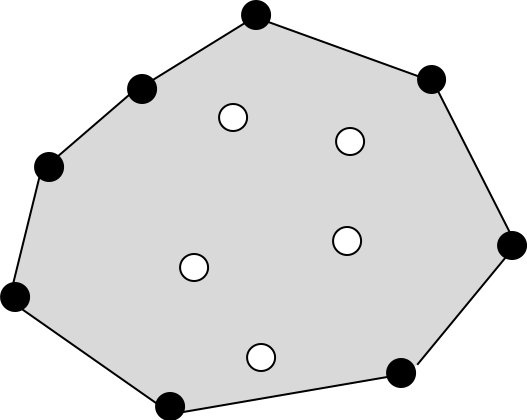
\includegraphics[width=0.5\linewidth]{figures-ext/convexhull} 

}

\caption[Convex hull illustration]{\textbf{Convex hull illustration}. A set of
points and its convex hull (line). Convex hull vertices are black, and
interior points are white. Image reproduced after \citet{Erickson2018}.}\label{fig:convexhull}
\end{figure}





Convex hull methods have been used in many fields, from economics and
engineering, I will discuss it with a focus on biological context to
link tightly to cell-type deconvolution.

The central assumptions of Convex hull optimization are that the gene
expression of pure cell types is non-negative and that cell type
proportions are linearly independent.

The shapes can be fitted to a cloud of points in many ways in order to
respond to given optimality criteria. A popular method introduced by
\citet{Shoval2012} and applied to gene expression and morphological
phenotypes of biological species employ the \textbf{Pareto front}
concept which aims to find a set of designs that are the best trade-offs
between different requirements.

Visually Pareto front correspond to the edge of the convex hull.

\citet{Wang2013} proposed Complex Analysis of Mixtures (CAM) method to
find the Pareto front (the vertices of \(X\) mixed matrix (a convex
set)). In the context of the cell-type deconvolution, it can be said
that ``the scatter simplex of pure subpopulation expressions is
compressed and rotated to form the scatter simplex of mixed expressions
whose vertices coincide with cell proportions''\citep{Wang2016}. In
respect to the assumptions, under a noise-free scenario, novel
\emph{marker genes} can be blindly identified by locating
the~\emph{vertices}~of the mixed expression scatter simplex
\citep{Wang2010}. In the figure (Fig. \ref{fig:cam}), the \(a_i\)'s are
cell-type proportions of \(k\) cell types, \(s_i\) pure cell type
expression and \(x_j\) mixed expression in sample \(j\). Therefore the
vertices correspond to the column vectors of the matrix \(A\) (Eq.
\eqref{eq:linear}). The genes placed in a distance \(d\) from the vertices
can be interpreted as marker genes.

\begin{figure}

{\centering 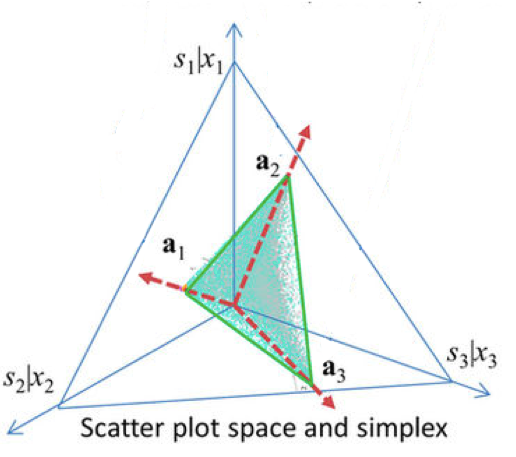
\includegraphics[width=0.5\linewidth]{figures-ext/cam} 

}

\caption[Fitting gene expression data of mixed populations to a convex hull shape]{\textbf{Fitting gene expression data of mixed
populations to a convex hull shape}. The geometry of the mixing
operation in scatter space that produces a compressed and rotated
scatter simplex whose vertices host subpopulation-specific marker genes
and corresponding to mixing proportions.}\label{fig:cam}
\end{figure}







In the procedure suggested by \citet{Wang2013}, before performing CAM,
clustering (more precisely affinity propagation clustering (APC) ) is
applied to the matrix in order to select genes representing clusters,
called cluster centers \(g_m\) and dimension reduction(PCA) is applied
to the sample space. Then in order to fit a convex set, a
margin-of-error should be minimized. The Eq. \eqref{eq:camErr} explains
the computation of the error which computes \(L2\) norm of the
difference between \(g_m\) possible vertices and remaining exterior
clusters. All possibilities of combinations drew from \(C^M_K\), \(M\)
number of clusters and \(K\) true vertices, are tested.

\begin{equation}
\begin{aligned}
\text{given }\alpha_k \geq 0, \sum^K_{k=1}\alpha_k=1 \\
\delta_{m, \{1,...,K\} \in C^M_K }= \underset{\alpha_k}{min} \sqrt{{g_m} - \sum^K_{k=1}\alpha_kg_k} \label{eq:camErr}
\end{aligned}
\end{equation}

Once optimal configuration is found, the proportions are computed using
standardised averaging: \begin{equation}
\hat{\alpha_k} = \frac{1}{n_{markers}} \sum_{i \in markers} \frac {x(i)}{\rVert x(i)\lVert}
\end{equation} where \(\hat{\alpha_k}\) is proportion of cell type
\(k\), \(n_{markers}\) number of marker genes (obtained from CAM), and
\(\rVert x(i)\lVert\) is the \(L1\) or \(L2\) norm of a given marker
gene \(x_i\).

Then the cell-type specific profiles are obtained with linear
regression. Authors of CAM also propose a minimum description length
(MDL) index that determines the number of sources in the mixture. It
selects the \(K\) minimizing the total description code length.

So far, the published R-Java package \emph{CAM} does not allow to
extract gene specific signatures, and it is not scalable to large
cohorts (many samples). In the article, authors apply essential
pre-processing steps that are not trivial to reproduce and which are not
included in their tool. Authors apply CAM and validate on rather simple
mixtures (tissue \emph{in vitro} mixtures and yeast cell cycle).

A slightly different approach was proposed by \citet{Newberg2018}. It
does not require initial dimension reduction steps or clustering before
fitting the convex hull, and it is based on a probabilistic framework.
The toll \emph{CellDistinguisher} was inspired by topic modeling
algorithm \citep{Arora2013}. It first computes \(Q\) matrix (Eq.
\eqref{eq:q}). Then each row vector of \(Q\) is normalized to 1 giving
\(\overline{Q}\) matrix. Every row of \(\overline{Q}\) lies in the
convex hull of the rows indexed by the cell-type specific genes. Then
\(L_2\) norm of each row is computes. Genes which rows have the highest
norm can be used as \emph{distinguishers} or \emph{marker} genes. Then
other runs of selections are applied after recentering the matrix to
find more markers.

\begin{equation}
Q=XX^T \label{eq:q}
\end{equation}

Once the set of possible distinguishers is defined, proportions and cell
profiles are computed using a Bayesian framework to fit the convex hull.
Authors provide a
\href{https://github.com/GeneralElectric/CellDistinguisher}{user-friendly
R package \emph{CellDistinguisher}}. Unfortunately, they do not provide
any method for estimation of some sources, which is critical for source
separation of complex tissues. Additionally, quantitative weights are
provided only for signature genes which number can vary for different
sources, and can be as small as one gene. Authors do not apply their
algorithm to complex mixtures as tumor transcriptome; they establish a
proof of concept with \emph{in vitro} mixtures of tissues.

The convex hull-based method does not require the independence of cell
types assumption, nor the non-correlation assumption which can be
interesting in the setup of closely related cell types. In theory, they
also allow \(k>j\) (more sources than samples). So far, the existing
tools are not directly applicable to tumor transcriptomes.

\hypertarget{matrix-factorization-methods}{%
\subsection{Matrix factorization
methods}\label{matrix-factorization-methods}}

Matrix factorization is a general problem not specific to cell types
deconvolution. It has been extensively used for signal processing
\citep{Zinovyev2013}and extraction of features from images
\citep{Hastie2009}. Matrix factorization can also be called BSS or
dimension reduction. Despite quite simple statistical bases they have
been proven to be able to solve quite complex problems. Many matrix
factorization methods can solve the problem of Eq. \eqref{eq:linear}. They
can solve it in different ways and concern different hypotheses.

Naturally, matrix factorization methods estimate simultaneously \(A\)
and \(S\) matrices (cell proportions and profiles) given \(X\)
rectangular matrix (genes \(\times\) samples) without any additional
input.

\begin{figure}

{\centering 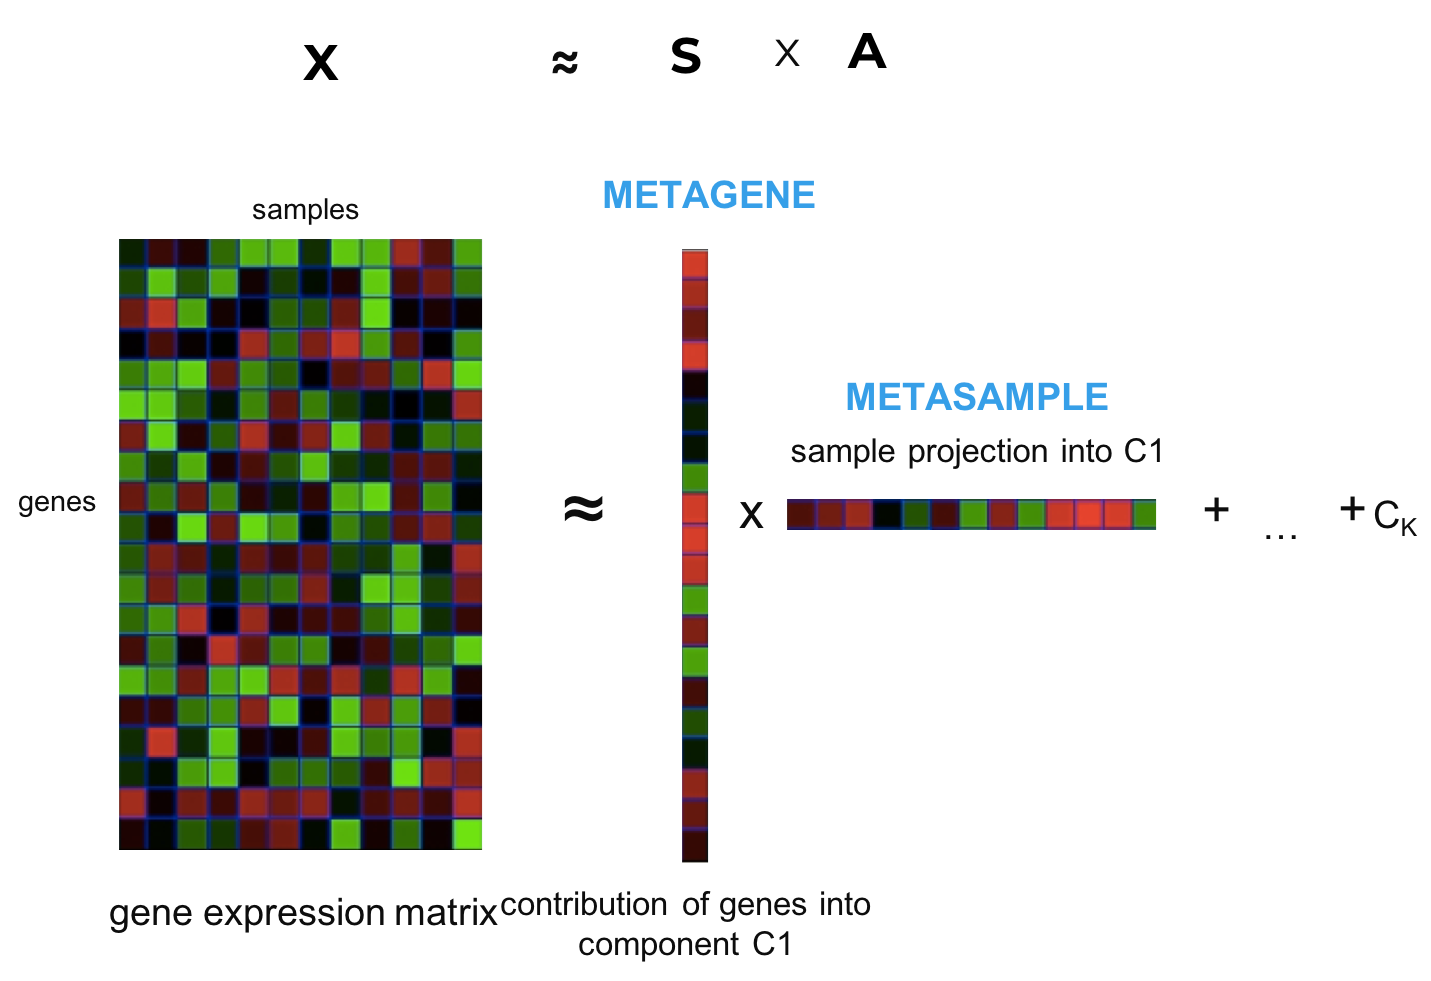
\includegraphics[width=1\linewidth]{figures-ext/factor} 

}

\caption[Principle of matrix factorisation of gene expression]{\textbf{Principle of matrix factorisation of gene
expression}. The gene expression matrix \(X\) is decomposed into a set
of \emph{metagenes} \(S\) matrix and \emph{metasamples} \(A\). Number of
components \emph{C} is defined with parametre \(k\).}\label{fig:fact}
\end{figure}






\hypertarget{principal-components-analysis}{%
\subsubsection{Principal Components
Analysis}\label{principal-components-analysis}}

One of the most popular methods, \textbf{Principal Components Analysis}
(PCA) computes projections of the variables onto the space of the
eigenvectors of the empirical covariance matrix, the projections are
mutually uncorrelated and ordered in variance. The principal components
provide a sequence of best linear approximations to that data.

PCA can be computed through eigen decomposition of the covariance
matrix. Covariance matrix is computed as follows:

\begin{equation}
\Sigma = \frac{1}{n-1}((X-\bar{x})^T(X-\bar{x})) \label{eq:covPCA}
\end{equation}

where \(\bar{x}\) is mean vector of the feature column in the data
\(X\).

Then the matrix is decomposed to eigenvalues: \begin{equation}
\mathbf{V^{-1}\Sigma V=D} \label{eq:eigenvecPCA}
\end{equation}

where \(\mathbf{V}\) is the matrix of eigenvectors and the
\(\mathbf{D}\) diagonal matrix of eigenvalues.

It can be also computed using \textbf{singular value decomposition}
(SVD) (computationally more efficient way):

\begin{equation}
X= UDV^T \label{eq:svd}
\end{equation}

Here \(U\) is an \(N \times p\) orthogonal matrix (\(U^T U = I_p\))
whose columns \(u_j\) are called the left singular vectors; \(V\) is a
\(p \times p\) orthogonal matrix (\(V^T V = I_p\)) with columns \(v_j\)
called the right singular vectors, and \(D\) is a \(p \times p\)
diagonal matrix, with diagonal elements
\(d_1 \geq d_2 \geq ... \geq d_p \geq 0\) known as the singular values.
The columns of \(UD\) are called the projections of principal components
of \(X\) on axes.

PCA finds directions in which the samples are dispersed to define
Principal Components. This dispersion is measured with variance, and
resulting PCA components are variance-ordered.

As nicely described in \citep{Rutledge2013}

\begin{quote}
\emph{The first PC is the vector describing the direction of maximum
sample dispersion. Each following PC describes the maximal remaining
variability, with the additional constraint that it must be orthogonal
to all the earlier PCs to avoid it contains any of the information
already extracted from the data matrix. In other words, each PC extracts
as much remaining variance from the data as possible. The calculated PCs
are weighted sums of the original variables, the weights being elements
of a so-called loadings vector. Inspection of these loadings vectors may
help determine which original variables contribute most to this PC
direction. However, PCs being mathematical constructs describing the
directions of greatest dispersion of the samples, there is no reason for
the loadings vectors to corresponding to underlying signals in the
dataset. Most of the time, PCs are combinations of pure source signals
and do not describe physical reality. For this reason, their
interpretation can be fraught with danger.}
\end{quote}

Especially in the context of the cell-type deconvolution, it can imagine
that different cell-types contribute to the variance, but one PC could
explain the joint variance of many cell types.

\citet{Wang2015} used SVD to compute matrix inversion in order to
separate tumor from the stroma. The method was applied to tumor
transcriptomes and gives purity estimation quite different from other
popular enrichment-based method ESTIMATE \citep{Yoshihara2013}.

\citet{Nelms2016} in CellMapper uses a semi-supervised approach based on
SVD decomposition to dissect human brain bulk transcriptome. Authors
define a query gene (a specific known gene), and then they decompose
transcriptome into components (eigenvectors) and multiply by weights
that are higher for the components correlated with the query gene. Then
the matrix is transformed back to gene \(\times\) samples matrix, but
query signal is amplified. The point is to find marker genes that
characterize the same cell-type as the query gene. Authors did not aim
at the identification of cell-type proportions or cell types profiles
but identification of cell-type specific markers. They underline
applicability of the method to rare cell types where many markers are
not available. This approach was proposed by authors to be used to
prioritize candidate genes in disease susceptibility loci identified by
GWAS.

\hypertarget{non-negative-matrix-factorisation}{%
\subsubsection{Non-negative matrix
factorisation}\label{non-negative-matrix-factorisation}}

Non-negative matrix factorization \citep{Seung1999} is an alternative
approach to principal components analysis. It requires data are
non-negative and it estimates components that are non-negative as well.
It finds its application in image analysis and gene expression analysis
where analyzed data are non-negative. The \(N \times p\) data matrix
\(X\) is approximated by

\[X \approx WH \]

where \(W\) is \(N \times r\) and \(H\) is \(r \times p\),
\(r ≤ max(N,p)\). We assume that \(x_{ij}\) ,\(w_{ik}\),
\(h_{kj}\)\(\geq 0\).

Which is a special case of Eq. \eqref{eq:linear}.

The matrices \(W\) and \(H\) are found by maximizing \begin{equation}
\mathcal{L}(W, H) = \sum^N_{i=1}\sum^{p}_{j=1}[x_{ij} log(WH)_{ij} − (WH)_{ij} ] \label{eq:nmf}
\end{equation}

The log-likelihood from a model in which \(x_{ij}\) is drawn from a
pre-defined distribution (i.e., Poisson) with a mean \((WH)_{ij}\).

This formula can be maximized through minimization of divergence:

\begin{equation}
\underset{W,H}{min} f(W,H)  = \frac{1}{2}\rVert X-WH\rVert^2_F \label{eq:divNMF}
\end{equation}

Where \(\rVert .\rVert_F\) is Frobenius norm, which can be replaced by
Kullback-Leibler divergence.

The optimization can be done employing different methods:

\begin{itemize}
\tightlist
\item
  \textbf{euclidean} update with multiplicative update rules, it is the
  classic NMF \citep{Seung1999} \begin{equation}
  \begin{aligned}
  W \leftarrow W \frac{XH^T}{WHH^T}\\H \leftarrow H\frac{W^TX}{W^TWH}  \label{eq:euclidNMF} 
  \end{aligned}
  \end{equation}
\item
  \textbf{alternating least squares} \citep{Paatero1994} where the
  matrices W and H are fixed alternatively
\item
  \textbf{alternating non-negative least squares} using projected
  gradients (\citet{Lin2007})
\item
  \textbf{convex-NMF }\citep{Ding2010} imposes a constraint that the
  columns of \(W\) must lie within the column space of~\(X\),
  i.e.~\(W = XA\)~(where~\(A\)~is an auxiliary adaptative weight matrix
  that fully determines~\(W\)), so that \(X=XAH\).~In this method only
  \(H\) must be non-negative.
\end{itemize}

The NMF algorithms can differ in initialization method as well and even
in situations where \(X = WH\) holds exactly, and the decomposition may
not be unique. This implies that the solution found by NMF depends on
the starting values. The performance of different combinations applied
to MRS data from human brain tumors can be found in
\citet{OrtegaMartorell2012}.

\citet{Brunet2004} created an NMF Matlab toolbox and demonstrated
applicability of NMF (using Kullback-Leibler divergence and euclidean
multiplicative update \citep{Lee2000} to cancer transcriptomes with
focus on cancer subtyping (focusing on the \(H\) matrix).
\citet{Brunet2004} also proposed a way to evaluate the optimal number of
factors (sources) to which matrix should be decomposed.

NMF as imposing non-negativity in the context of decomposition of
transcriptomes seems as an attractive concept as both cell profiles and
cell proportions should be non-negative. It is not surprising then that
some authors used NMF to perform cell-type deconvolution.

To my knowledge, \emph{deconf} \citep{Repsilber2010} was the first tool
proposing NMF cell-type deconvolution of PBMC transcriptome, of
considerable dimensions, 80 samples (40 control and 40 cases) of
Tuberculosis. \citet{Repsilber2010} employed random initialization and
alternating non-negative least squares to minimize the model divergence.
The complete deconvolution of the transcriptome was used to perform DEG
analysis on the deconvoluted profiles.

\citet{Shen-Orr2013}, not only presented exhaustive literature review
through implementing cell-type deconvolution methods in an R package
\emph{CellMix} \citep{Gaujoux2013} but also proposed a semi-supervised
NMF for cell-type deconvolution and published an R package implementing
different NMF methods \citep{Gaujoux2010}. The semi-supervised version
of NMF proposed by \citet{Gaujoux2013}, need a set of specific marker
genes for each desired cell type. Then at initialization and after each
iteration of the chosen NMF algorithm (applies to some versions of NMF
\citep{Seung1999, Brunet2004, PascualMontano2006}, ``each cell type
signature has the values corresponding to markers of other cell types
set to zero. The values for its own markers are left free to be updated
by the algorithm's own iterative schema''. Applying their algorithm to
\emph{in vitro} controlled dataset {[}GSE11058 \citep{Abbas2009},
testing selected NMF implementations and a varying number of markers per
cell, authors observed the best performance with guided version of
\emph{brunet} \citep{Brunet2004} implementation.

\citet{Moffitt2015} applied NMF to separate tumor from stroma in
pancreatic ductal carcinoma (PDAC) using multiplicative update NMF. They
scaled \(H\) matrix rows to 1 so that the values correspond to the
proportions. Authors tested different possibilities of the number of
sources (\(k\)), the final number of factors was defined through
hierarchical clustering on gene-by-gene consensus matrix of top 50 genes
of each component.

Finally \citet{Liu2017} proposed post-modified NMF in order to separate
\emph{in vitro} mixtures of different tissues.

In brief, NMF is a popular, in biology, algorithm performing source
separation with non-negativity constraint. It was applied to \emph{in
vitro} cell-mixtures and blood transcriptomes, showing a satisfying
accuracy of cell-type \emph{in silico} dissection and evaluating
proportions. It was also applied in cancer context. However, it did not
recover cell-type specific signals but rather groups of signals that
could be associated with cancer or stroma.

\hypertarget{independent-components-analysis}{%
\subsubsection{Independent Components
Analysis}\label{independent-components-analysis}}

Independent Components Analysis is written as in Eq. \eqref{eq:linear}
maximizing \emph{independence} and \emph{non-Gaussianity} of columns of
\(S\): \(S_i\). It was first formulated by \citet{Herault1986}

The independence can be measured with entropy, kurtosis, mutual
information or negentropy measure \(J(Y_j )\) \citep{Hyvarinen2000}
defined by

\begin{equation}
J(Y_j ) = H(Z_j ) - H(Y_j ) \label{eq:negentropy}
\end{equation}

where \(H(Y_j )\) is entropy, \(Z_j\) is a Gaussian random variable with
the same variance as \(Y_j\). Negentropy is non-negative and measures
the deviation of \(Y_j\) from Gaussianity. An approximation of
negentropy is used in popular implementation of \textbf{FastICA}
\citep{Hyvarinen2000}. Other existing implementations of ICA are

\begin{itemize}
\tightlist
\item
  Infomax \citep{Bell1995} using Information-Maximization that maximizes
  the joint entropy
\item
  JADE (\citet{Cardoso1993}) on the construction of a fourth-order
  cumulants array from the data
\end{itemize}

However, they are usually a lot slower which limits their application to
a large corpus of data and \citet{Teschendorff2007} demonstrated that
\emph{FastICA} gives the most interpretable results.

Therefore, I will focus on FastICA implementation as it will be
extensively used in the \protect\hyperlink{results}{Results} part.

FastICA requires \emph{prewhitening} of the data (centering and
whitening). Centering is removing mean from each row of \(X\) (input
data). Whitening is a linear transformation that columns are not
correlated and have variance equal to 1.

\textbf{Prewhitenning }

\begin{enumerate}
\def\labelenumi{\arabic{enumi}.}
\tightlist
\item
  Data centering \begin{equation}
    x_{ij} \leftarrow x_{ij} - {\frac {1}{M}}\sum_{j^{\prime }}x_{ij^{\prime }}  \label{eq:cent}
    \end{equation} \(x_{ij}\): data point
\item
  Whitenning \begin{equation}
   \mathbf {X} \leftarrow \mathbf {E}\mathbf {D} ^{-\frac{1}{2}}\mathbf {E} ^{T}\mathbf {X} \label{eq:whit}
   \end{equation} Where \(\mathbf {X}\) - centered data, \(\mathbf {E}\)
  is the matrix of eigenvectors, \(\mathbf{D}\) is the diagonal matrix
  of eigenvalues
\end{enumerate}

\begin{algorithm}
\caption{ FastICA multiple component extraction}
\begin{algorithmic}[1]
\INPUT{$K $ Number of desired components}
\INPUT{$X \in \mathbb{R}^{N \times M}$ Prewhitened matrix, where each column represents an $N$-dimensional sample, where $K \leq N$ }
\OUTPUT{$A \in \mathbb{R}^{N \times K}$ Un-mixing matrix where each column projects  $\mathbf {X}$ onto independent component.}
\OUTPUT{$S \in \mathbb{R}^{K \times M}$ Independent components matrix, with $M$ columns representing a sample with $K$ dimensions.}
\begin{equation}\label{eq:fasticaMul}\end{equation}
\For{$p\gets 1, K$}
\State $\mathbf{w}_{p} \gets$ \emph{Random vector of length} $N$
\While{$\mathbf{w_{p}}$ \emph{ changes}}
\State $\mathbf{w}_p \gets \frac{1}{M}Xg(\mathbf{w}_p^TX)^T - \frac{1}{M}g'(\mathbf{w}_p^TX)1w_p$
\State $\mathbf{w}_p \gets \mathbf{w}_p - (\sum_{j=1}^{p-1}\mathbf{w}_p^T\mathbf{w}_j\mathbf{w}_j^T)^T$
\State $\mathbf{w}_p \gets \frac{\mathbf{w}_p}{\lVert \mathbf{w}_p \rVert}$
\EndWhile
\EndFor
\State where $\mathbf {1}$  is a column vector of 1's of dimension $M$
\OUTPUT{$A = [\mathbf{w}_1, ..., \mathbf{w}_K]$}
\OUTPUT{$S = \mathbf{A}^T\mathbf{X}$}
\end{algorithmic}
\end{algorithm}

However, the results of this algorithm (Alg. 1. \eqref{eq:fasticaMul}) are
not deterministic, as the \(\mathbf{w}_{p}\) initial vector of weights
is generated at random in the iterations of fastICA. If ICA is run
multiple times, one can measure \textbf{stability} of a component.
Stability of an independent component, regarding varying the initial
starts of the ICA algorithm, is a measure of internal compactness of a
cluster of matched independent components produced in multiple ICA runs
for the same dataset and with the same parameter set but with random
initialization \citep{Himberg2003}.

The Icasso procedure can be summarized in a few steps :

\begin{enumerate}
\def\labelenumi{\arabic{enumi}.}
\tightlist
\item
  applying multiple runs of ICA with different initializations
\item
  clustering the resulting components
\item
  defining the final result as cluster centroids
\item
  estimating the compactness of the clusters
\end{enumerate}

In brief, ICA looks for a sequence of orthogonal projections such that
the projected data look as far from Gaussian as possible. ICA starts
from a factor analysis solution and looks for rotations that lead to
independent components.

So far, ICA was used to deconvolute transcriptomes into biological
functions
\citep{Biton2014, Engreitz2010, Gorban2007, Teschendorff2007, Zinovyev2013}.
However, it has never been used for cell-type deconvolution.

In theory, ICA outputs: \(S\) could be interpreted as sources and \(A\)
as proportions in the cell-type deconvolution context. In practice, the
fact that the ICA allows negative weights of projections, it makes the
interpretation less trivial.

To my knowledge, my \protect\hyperlink{DeconICA}{DeconICA} R-package
(that will be described in the results part) is the first method
allowing interpretation of ICA-based signals as cell-type
context-specific signatures and quantify their abundance in the
transcriptome.

\begin{figure}

{\centering 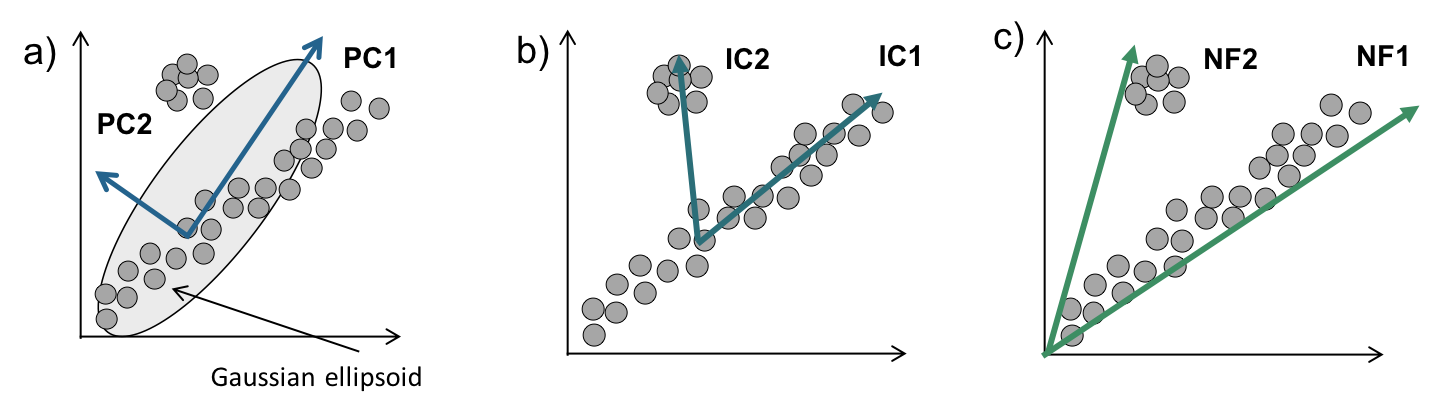
\includegraphics[width=0.8\linewidth]{figures-ext/bss} 

}

\caption[Simple illustration of matrix factorisation methods]{\textbf{Simple illustration of matrix
factorisation methods}. Adapted with permision from \citep{Zinovyev2013}}\label{fig:matrixfact}
\end{figure}




All in all, matrix factorization methods are able to decompose a gene
expression matrix into a weighted set of genes (metagene)(\(S\)) and
weighted set of samples (metasample \(A\)). Discussed here PCA, NMF and
ICA differ in constraints and starting hypotheses. PCA components are
ordered by variance and are orthogonal in the initial space of data
(Fig. \ref{fig:matrixfact} ). NMF impose non-negativity constraint and
ICA independence of sources hypothesis. Components of NMF and ICA are
not ordered. For all the matrix factorization methods number of
components (or factors) (\(k\)) needs to be given to the algorithm. Some
authors propose a way to estimate the optimal number of components
usually justified in a specific context. NMF and SVD were applied in the
context of cell-type deconvolution while ICA, so far, was used to
dissect transcriptome into factors related to signaling pathways,
technical biases or clinical features. Also, ICA was proven to find
reproducible signals between different datasets
\citep{Cantini2018, Teschendorff2007}. I am going to discuss this aspect
of the \protect\hyperlink{results-1}{Results} section.

\hypertarget{attractor-metagenes}{%
\subsection{Attractor metagenes}\label{attractor-metagenes}}

A method proposed by \citet{Cheng2013} that can be run in
semi-supervised or unsupervised mode is called attractor metagenes.
Authors describe their rationale as follows:

\begin{quote}
\emph{We can first define a consensus metagene from the average
expression levels of all genes in the cluster, and rank all the
individual genes in terms of their association (defined numerically by
some form of correlation) with that metagene. We can then replace the
member genes of the cluster with an equal number of the top-ranked
genes. Some of the original genes may naturally remain as members of the
cluster, but some may be replaced, as this process will ``attract'' some
other genes that are more strongly correlated with the cluster. We can
now define a new metagene defined by the average expression levels of
the genes in the newly defined cluster, and re-rank all the individual
genes concerning their association with that new metagene; and so on. It
is intuitively reasonable to expect that this iterative process will
eventually converge to a cluster that contains precisely the genes that
are most associated with the metagene of the same cluster so that any
other individual genes will be less strongly associated with the
metagene. We can think of this particular cluster defined by the
convergence of this iterative process as an ``attractor,'' i.e., a
module of co-expressed genes to which many other gene sets with close
but not identical membership will converge using the same computational
methodology.}
\end{quote}

Which in pseudocode works as described in Algorithm 2 \eqref{eq:attr} and
it is implemented in R code is available online in
\href{https://www.synapse.org/\#!Synapse:syn1446295}{Synapse portal}.

\begin{algorithm}
\caption{Attractor metagenes algorithm}
\begin{algorithmic}[2]
\INPUT{$\alpha$ shrinkage parameter}
\INPUT{$X \in \mathbb{R}^{N \times M}$ gene expression matrix}
\OUTPUT{$m_j$ metagene of $g_{seed}$ }
\begin{equation}\label{eq:attr}\end{equation}
\State{$g_{seed} \gets$ \emph{a gene from} $1:N$ }
 \State{$I^{\alpha}(g_{seed}; g_i)$} \Comment{compute association beteen $g_{seed}$ and $g_i$}
\State{$w_i = f(I^{\alpha}(g_{seed}; g_i))$} \Comment{compute weights for each gene}
\State{$m_0 = \frac{\sum^N-1_{i=1}(g_iw_i)}{\sum^N-1_{i=1}w_i} $}\Comment{compute metagene as weighted average of all genes}
\State{$I^{\alpha}(m_0; g_i)$} \Comment{compute association between metagene $m_0$ and each gene $g_i$}
 \Repeat
\State{$w_i = f(I^{\alpha}(m_0; g_i))$}
 \State{$m_j = \frac{\sum^N-1_{i=1}(m_0w_i)}{\sum^N-1_{i=1}w_i} $}
\Until {$m_{j+1} =  m_j$}
\end{algorithmic}
\end{algorithm}

The produced signatures' weights are non-negative. In the original
paper, the generation of tumor signatures leads to three reproducible
signatures among different tumor types, including \emph{leucocyte}
metagene. Typically with the essential parameter \(\alpha=5\), they
discovered typically approximately 50 to 150 resulting attractors.

This method was further to study breast cancer \citep{AlEjeh2014} and to
SNP data \citep{Elmas2016}.

There is a possibility to tune the \(\alpha\) parameter in order to
obtain more or less metagenes that would be possibly interpretable as
cell-type signatures.

\hypertarget{others-aspects}{%
\subsection{Others aspects}\label{others-aspects}}

Here I will discuss transversal aspects common to most deconvolution
methods. They play the critical role in the final results and are often
omitted while algorithms are published which impacts the reproducibility
significantly.

\hypertarget{types-of-biological-reference}{%
\subsubsection{Types of biological
reference}\label{types-of-biological-reference}}

Let us consider the case of the deconvolution where neither \(A\) or
\(S\) are not known (Eq. \eqref{eq:linear}) (as in the case of cancer
transcriptomes), and we would like to estimate cell proportions or both
cell proportions and cell profiles. No matter if the method is
supervised or unsupervised at some point of the protocol the biological
knowledge about cell types is necessary in order to either derive the
model or interpret the data. I discussed signatures from the biological
perspective in Section \ref{immune-signatures}. Here, I would like to
stress the importance of the design of gene signatures which aim is to
facilitate cell-type deconvolution.

Depending on chosen solution different type of reference can be used. In
regression algorithms, a way to approximate the individual cell-type
profiles is necessary to estimate proportions. However, the genes that
are the most variant between cell types are enough for regression, and
not all profiles are necessary. A matrix containing gene expression
characteristic for a set of cell-types, often for selected, most
discriminative, genes is called \textbf{basis matrix}. The choice of the
genes and the number of the genes impact the outcome
\citep{Vallania2017} significantly. Therefore, most of the regression
methods come together with a new basis matrix, ranging from hundreds to
tens of genes. Typically, genes selected for basis matrix should be
cell-type specific in respect to other estimated cell types, validated
across many biological conditions \citep{Hoffmann2006}.
\citet{Racle2017} adds a weight directly in the regression formula (see
Eq. \eqref{eq:epic} ) that corresponds to the variability of a signature
gene between independent measurements of the same cell type so that the
least inter-cell type variable genes have more weight in the model.
\emph{CellMix} \citep{Gaujoux2013} regroups different indexes to select
the most specific genes based on signal-to-noise ratio. However, the
most popular method is the selection of differentially expressed genes
between pure populations. Often criteria for the optimal number of genes
in the basis matrix are not knowledge-based but data-driven.
\citet{Abbas2009} uses matrix mathematical property - condition number
of basis matrix (\emph{kappa}) in order to select the number of genes.
CIBERSORT and many other regression methods follow the same approach.
\citet{Newman2015} also added another step while constructing the basis
matrix, and it preselects reference profiles having maximal
discriminatory power. Some authors \citep{Ju2013, Nelms2016} propose to
find marker genes through correlation with a provided marker gene (a
single one or a group of genes).

In enrichment methods, \textbf{gene list} can be enough to estimate cell
abundance, sometimes (i.e., GSEA) ranked gene list is necessary. The
choice of extremely specific markers is crucial for accurate call-type
abundance estimation. The choice of markers can also be
platform-dependent, this point is strongly underlined in
\citep{Becht2016}. An interesting possibility is the use of gene list of
different \emph{cell states} in order obtain coarse-grain resolution.

The impact of missing gene from a signature in the bulk dataset remains
an unanswered question. It would be logical that shorter the gene list
for a specific cell, a lack of a gene can have more impact on the
result. There is a need for an accurate threshold between robustness and
accuracy of the method.

In unsupervised methods, purified cell-profiles, signatures or list of
genes can be used \emph{\textbf{a posteriori}} to interpret the obtained
sources. Even though the choice of reference does not affect the
original deconvolution, it affects the interpretation. The advantage of
\emph{a posteriori} interpretation is a possibility to use different
sources and types of signatures in order to provide the most plausible
interpretation. It is common that the way of interpretation of
components is not included in the deconvolution tool
\citep[\citet{Newberg2018}, \citet{Moffitt2015}]{Wang2016}, even though
it is a crucial part of the analysis.

For the deconvolution of tumoral biopsies, most of the reference
profiles, up to now, are coming from the blood, which is the most
available resource. Therefore most of the methods make a hypothesis that
blood cell-type profiles/signatures are a correct approximation of
cancer infiltrating immune cells. Rare models like PERT \citep{Qiao2012}
or ImmuneStates \citep{Vallania2017} discuss the perturbation of the
blood-derived profiles in diseases.

With the availability of single-cell RNA-seq of human cancers
\citep{Chung2017, Lavin2017, Li2017, Puram2017, Schelker2017, Tirosh2016, Zheng2017},
we gain more knowledge on immune cells in TME, and there is growing
evidence that they differ importantly from blood immune cells.
\citet{Racle2017} show that lymph node-resident immune cells have
expression profile closer to blood immune cells than cancer immune
cells. \citet{Schelker2017} shows, using a synthetic bulk dataset that
using single cell profiles with existing regression methods (CIBERSORT)
can improve their performance in the cancer context. However,
availability of scRNA-seq remains succinct and probably do not embrace
the patient heterogeneity that can be found in large bulk transcriptome
cohorts.

\hypertarget{data-processing}{%
\subsubsection{Data processing}\label{data-processing}}

Data pre- and post-processing can have a substantial impact on the
deconvolution. Many authors apply strong filtering of genes
\citep{Wang2016}, removing probes with the lowest and the highest
expression (potential outliers). In many cases, data preprocessing is
not detailed and therefore impossible to reproduce.

There is also a debate on the data normalization.

In microarray analysis pipeline, data are transformed into log-space,
usually \(log_2(x+1)\) in order to make the distribution closer to
Gaussian and therefore facilitate statistical hypothesis testing
\citep{Hoyle2002}. It also stabilizes the variance \citep{Tsai2003}.

Most of the authors suggest to use counts (not transformed into
log-space) for estimating cell abundance as log-transformed data violate
the linearity assumption \citep{Zhong2013}, some opt against it
\citep{Shannon2017, Clarke2010}, and some envisage both possibilities
\citep{Erkkila2010, Repsilber2010}.

For the RNA-seq data TPM (transcripts per million) normalization is
preferred or even required by most methods
\citep{Chen2018, Finotello2017, Racle2017}. \citet{Jin2017} performed an
extensive analysis of RNA-seq data processing that preserves best the
linearity for deconvolution suggesting that TPM normalization for
deconvolution studies.

For matrix factorization: PCA, ICA the data are usually log-transformed
and centred to reduce the influence of extreme values or outliers. NMF
for cell-type deconvolution is usually applied in non-log space.

\hypertarget{Validation}{%
\subsubsection{Validation}\label{Validation}}

Most of algorithm validation starts with \emph{in silico} mixtures (Fig.
\ref{fig:dataVal}). In published articles, the bulk transcriptome is
simulated in two ways (1) mixing numerically simulated sources at
defined proportions of given distribution (i.e.~uniform) using linear
model (for instance NMF) (2) using sampling (for instance Monte Carlo)
to randomly select existing pure profiles and mixing them (additive
model) at random proportions. To the obtained bulk samples, noise can be
added at different steps of the simulation. Additional parameters can be
defined in \emph{in silico} mixtures, for instance, CellMix allows
defining the number of marker genes (specific to only one source) for
each cell type. The simulated benchmark based on single cell data was
used in \citet{Schelker2017} and \citet{Gortler2018}. In this framework,
simulated data was obtained through summing single cell profiles at
known proportions. The main pitfall of those methods is that in the
proposed simulations the gene covariance structure is not preserved. In
reality, the proportions of cell types are usually not random, and some
immune cell types can be correlated or anti-correlated. In addition,
these simulations create a simple additive model which perfectly agrees
with the linear deconvolution model. This is probably not the case of
the real bulk data affected by different factors as cell cycle,
technical biases, patients heterogeneity and especially cell-cell
interactions.

\begin{figure}

{\centering \includegraphics[width=1\linewidth]{figures-ext/dataVal} 

}

\caption[From theory to practice: simplified pipeline of model validation]{\textbf{From theory to practice: a simplified
pipeline of model validation}. The scheme reflects pipeline of data
validation commonly used in transcriptome deconvolution methods
validation. The project can be started from a biological problem (A) and
then a way to solve the problem in mathematical model (C) is tested.
Most commonly, the project starts with the model (C) then it is tested
on simulated data (D). Next level of difficulty is testing the model
with real data, so-called, benchmark data (B) that were generated in
some biological context different from initial problem. They need to be
usually normalized (E) before the model is challenged. B data are widely
used as they are easily available and there is some validation available
facilitating comparison. Lastly, it is assumed that if the method works
fine in the context B, it will work as well in the context A, preferably
accompanied by some partial validation. One can replace A by cancer
transcriptomics, B by blood data or \emph{in vitro} mixtures if the
focus is TME bulk transcriptomics deconvolution.}\label{fig:dataVal}
\end{figure}


















Naturally, algorithms validated with simulated mixtures are then
validated with controlled \emph{in vitro} mixtures of cell types or
tissues mixed in known proportions. The most popular benchmark datasets
are:

\begin{itemize}
\tightlist
\item
  mix of human cell lines Jurkat, THP-1, IM-9 and Raji in four different
  concentration in triplicates and the pure cell-line profiles
  (\href{https://www.ncbi.nlm.nih.gov/geo/query/acc.cgi?acc=GSE11058}{GSE11058})
  \citep{Abbas2009};
\item
  mix of rat tissues: liver, brain, lung mixed in 11 different
  concentrations in triplicates and the pure tissues
  expression(\href{https://www.ncbi.nlm.nih.gov/geo/query/acc.cgi?acc=GSE19830}{GSE19830})
  \citep{ShenOrr2010}
\end{itemize}

Similar simple mixtures are also proposed by other authors
\citep[\citet{Kuhn2011}]{Becht2016}. This type of benchmark adds the
complexity of possible data processing and experimental noise. However,
it still follows an almost perfect additive model as the cell/tissues do
not interact and they are only constituents of the mixture.

Several tools performed systematic benchmark using PBMC or whole blood
datasets, where for a number of patients (that can be over one hundred)
FACS measured proportions of selected cell types and bulk transcriptomes
are available. Many such datasets can be found at
\href{http://www.immport.org/immport-open/public/home/home}{IMMPORT}
database. \citet{Aran2017} kindly shared with scientific community two
datasets with a considerable number of patients (\(\sim80\) and
\(\sim110\)) and processed FACS data (actual proportions) on their
\href{https://github.com/dviraran/xCell/blob/master/Dev_scripts/xCell_ImmPort.zip}{github
repository}. It is still important to remember that liquid tissues are
easier to deconvolute and for the tools using \emph{a priori} reference,
the reference profiles are obtained from the blood. Therefore the
context remains consistent.

For the solid cancer tissues deconvolution, some of the tools were
validated with the stained histopathology cuts using in
situ-hybridisation (ISH) \citep{Kuhn2011} or immunohistochemistry (IHC)
(\citet{Becht2016}). Often this method estimates a limited number of
cell types and the measured abundance of pictures can also be biased by
the technical issues (image/ staining quality).

Authors of EPIC validated their tool with paired RNAseq and Lymph node
FACS-derived proportions in 4 patients
(\href{https://www.ncbi.nlm.nih.gov/geo/query/acc.cgi?acc=GSE93722}{GSE93722}).
They also noticed that it is more straightforward to correctly evaluate
lymph node immune cell types than cancer infiltrating cell types as
lymph node-resident cells are more similar to the blood immune cells.

FACS and gene expression of blood cancer (Follicular lymphoma) were also
used by \citet{Newman2015} for 14 patients (unpublished data). For solid
tissues, \citet{Newman2015} used paired FACS and expression datasets of
normal lung tissues for B-cell and CD8 and CD4 T cells of 11 patients
(unpublished data).

Some authors proposed to cross-validate estimated proportions with
estimated proportions based on a different data input (i.e., methylome)
\citep[\citet{Senbabaoglu2016}]{Li2016} or CNA
(\citet{Senbabaoglu2016}). This type of validation is interesting, even
though in many projects only one type of data types are available for
the same samples. TCGA data is one of few exceptions.

Finally, a validation of deconvolution of solid cancer tissues remains
incomplete as no paired expression and FACS data is available up to
date.

\hypertarget{statistical-significance}{%
\subsubsection{Statistical
significance}\label{statistical-significance}}

A little number of tools propose a statistical significance assessment.
CIBERSORT computes empirical p-values using Monte Carlo sampling. Infino
authors \citep{Zaslavsky2017} provide a confidence interval for the
proportion estimations. This allows knowing which proportion estimation
are more trustful than other.

Most tools compare themselves to others measuring the accuracy of the
prediction, or Pearson correlation, on the benchmark datasets (described
above). Often, in the idealized mixtures, methods perform well.
Evaluation of their performance in cancer tissues remains unanswered
without proper statistical evaluation.

\hypertarget{summary-2}{%
\subsection{Summary}\label{summary-2}}

The field of computational transcriptome deconvolution is continuously
growing. Initially used to solve simple in vitro or simulated mixtures
of quite distinct ingredients, then to deconvolute blood expression
data, finally applied to solid cancer tissues. In cancer research,
digital quantification of cancer purity becomes a routine part of big
cancer research projects \citep{Yoshihara2013}. Cell-type
quantification, even though the validation framework and statistical
significance of deconvolution tools can still be improved, seems to be
considered as a popular part of an analytical pipeline of bulk tumor
transcriptomes \citep{Cieslik2017}. Different types of approaches try to
solve the deconvolution problem, focusing on different aspects of the
quantification, or proposing methodologically different approaches.
Methods proposing an unsupervised solution to the deconvolution problem
of transcriptomes are still underrepresented. All the tools assume a
linear additive model without explicitly including the impact of
possible interactions on the cell-type quantification. The tools that
met the most prominent success were proven by the authors to be readily
applicable to a variety of cancer datasets and reusable without an extra
effort (through a programming library or web interface). The field is
still waiting for a gold standard validation benchmark that would allow
a fair comparison of all the tools in solid cancer tissues. It is also
remarkable that the recent methods focus on quantification of the
abundance of an average representation of cell-types without aspiring to
deconvolute the cell-type context-specific profiles. Thanks to various
cancer single-cell data and big-scale projects \citep{Regev2017}, we
will be able to improve the existing deconvolution approaches and
finally replace the collection of bulk transcriptomes by a collection of
scRNA-seq ones.

\hypertarget{otherDecon}{%
\section{Deconvolution of other data types}\label{otherDecon}}

The transcriptome data is not the unique omic data type that can be used
to infer cell type proportions. Genomic and epigenomic data was used in
numerous publications to perform cell-type deconvolution or estimate
sample purity. I will present a general landscape of the tools and
methods used for this purpose.

\hypertarget{dna-methylation-data}{%
\subsection{DNA methylation data}\label{dna-methylation-data}}

Cell-type composition can be computed from DNA methylation data
(described in \protect\hyperlink{epi}{Section X}). In EWAS (Epigenome
Wide Association Studies) variation origination from cell types is
considered as an important confounding factor that should be removed
before comparing cases and controls and defining Differentially
Methylated Positions (DMPs). \citet{Teschendorff2017} reviewed ten tools
for epigenome deconvolution. Authors identify six of the described
methods as reference-free (which I called in this Chapter
\emph{unsupervised}), three are regression-based, and one is
semi-supervised. Another review on this topic was authored by
\citet{Titus2017}.

Unsupervised methods employed in methylome cell-type deconvolution are
RefFreeEWAS \citep{Houseman2014}, SVA \citep{Leek2007} are based on SVD,
ISVA based on ICA {[}\citet{Teschendorff2011}) are more general methods
that aim to detect and remove confounders from the data (that do not
need to be necessary the cell types). RUVm \citep{Maksimovic2015} is a
semi-supervised method using generalized least squares (GLS) regression
with negative reference also used to remove \emph{unwanted variation}
from the data and could be potentially adapted to cell-type
deconvolution. EWASher (\citet{Zou2014}) is linear mixed model and PCA
based method that corrects for cell-type composition. Similarly,
ReFACTor \citep{Rahmani2016} use sparse PCA to remove the variation due
to cell-type proportions. \citet{Houseman2016} proposed RefFreeCellMix:
an NMF model with convex constraints to estimate factors representing
cell types and cell-type proportions and a likelihood-based method of
estimating the underlying dimensionality~(\(k\) number of factors). A
different tool MeDeCom \citep{Lutsik2017} uses alternating non-negative
least squares to fit a convex hull.

As far as supervised methods are concerned, EPiDISH
(\emph{E}pigenetic~\emph{D}issection
of~\emph{I}ntra-\emph{S}ample-\emph{H}eterogeneity) R-package
\citep{Teschendorff2017} includes previously published tools: Quadratic
programming method using reference specific DNAse hypersensitive sites
{[}Constrained Projection (CP) \citep{Houseman2012}), adapted to
methylome deconvolution CIBERSORT algorithm (\(\nu\)-SVR) and robust
partial correlations~(RPC) method (a form of linear regression).
Reference cell-type specific profiles were obtained from the blood.

eFORGE \citep{Breeze2016} can detect in a list of DMPs if there is a
significant cell-type effect.

EDec \citep{Onuchic2016} uses DNAm to infer factors proportions using
NMF and then derives factors profiles though linear regression of
transcriptome data of cancer datasets. Authors identify the tumor and
stroma compartments and profiles. However, they admit the error rate for
profiles is quite high for most genes.

\citet{Wen2016} focused on intra-tumor heterogeneity (clonal evolution)
based on DNAm data. Profiles obtained from cell lines were used in a
regression model to identify the proportions of sub-clones in breast
cancer data. InfiniumPurify \citep{Zheng2017} and LUMP \citep{Aran2015}
uses DNAm to estimate sample purity.

The validation framework for methylation deconvolution is very similar
to transcriptome ones: in silico mixtures and FACS-measured proportions
of the blood. Most of the tools assume the cell composition is a factor
the most contributing to the variability and therefore SVD/PCA based
approaches are sufficient to correct for the variability. According to
\citet{Teschendorff2017}, this assumption was not proven to hold true in
solid tissues like cancer. Supervised methods have the same drawback as
in the case of the transcriptome, and they use purified profiles from
one context to derive cell proportions in a different context. In
overall, it seems that no study proposed cell-type quantification based
on methylome profiles in a pan-cancer manner.

\hypertarget{copy-number-aberrations-cna}{%
\subsection{Copy number aberrations
(CNA)}\label{copy-number-aberrations-cna}}

To my knowledge there is no method using CNA data in order to estimate
cell-type composition, as CNA occur in tumor tissue and natural
distinction can be made between tumor and normal cells and within tumor
cells (intra-tumor).

Therefore, copy number aberrations can be used to estimate tumor purity
and clonality. BACOM 2.0 \citep{Fu2015}, ABSOLUTE \citep{Carter2012},
CloneCNA \citep{Yu2016}, PureBayes \citep{Larson2013}, CHAT
\citep{Li2014}, ThetA \citep{Oesper2013}, SciClone \citep{Miller2014},
Canopy \citep{Jiang2016}, PyClone \citep{Roth2014}, EXPANDS
\citep{Andor2014} estimate tumor purity and quantify true copy numbers.
\href{https://omictools.com/tumor-purity-and-heterogeneity-category}{OmicTools
website} reports 70 tools serving this purpose and their review goes
beyond the scope of my work. Most tools use tumor and normal samples,
paired if possible.
\href{https://github.com/DeveauP/QuantumClone/}{QuantumClone} seem to be
the only tool that requires a few samples from the same tumor (in time
or space dimension).

\citet{Aran2015} published Consensus measurement of purity estimation
that combines purity estimations based on different data types
(available in \href{http://www.cbioportal.org/}{cBioportal}) using:
ESTIMATE \citep{Yoshihara2013} (gene expression data), ABSOLUTE
\citep{Carter2012} (CNA), LUMP \citep{Aran2015} (DNAm and IHC of stained
slides. Authors concluded that the estimation based on different data
types highly correlate with each other, besides the IHC estimates, which
suggests that IHC provides a qualitative estimation of purity.

\hypertarget{summary-of-the-chapter-1}{%
\section{Summary of the chapter}\label{summary-of-the-chapter-1}}

A plethora of machine learning solutions has been developed to solve
problems of different nature. Supervised and Unsupervised approaches can
be distinguished depending if a model is provided a set of training data
with known response or the algorithm works blindly trying to find
patterns in the data. Some of the algorithms found an essential
application in healthcare and are included in the clinical routine.

One of the critical problems that can, in theory, be solved with ML, is
bulk omic data deconvolution. Different types of deconvolution of cancer
samples can be distinguished: clonal, purity and cell-type
deconvolution. Here I focused on cell-type deconvolution of
transcriptome data. Through an extensive review, I presented 64 tools
and divided them into categories depending on the adapted type of
approach. I distinguished probabilistic, enrichment-based,
regression-based, convex hull, matrix factorization and attractor
metagene approaches that can be used for cell-type deconvolution. I
detailed the basis of the different models and highlighted the most
important features counting for cell-type deconvolution.

DNAm data were also used to estimate cell-type proportions. However, the
heterogeneity found in methylome data resulting from the difference in
cell type proportions is usually seen as a confounding factor to be
removed. CNA data can be used for estimation of tumor purity and
clonality.

In brief, for the transcriptome cell-type deconvolution, it can be
observed that just a limited number of tools are usable in practice in
order to deconvolute large cancer cohorts and without the need to
provide hard to estimate parameters. Supervised methods applied to
cancer use reference-profiles coming from a different context.
Unsupervised tools, so far, are somewhat underrepresented in the field
and do not offer a solution directly applicable to cancer transcriptomes
of high dimensions. All of the presented methods are still waiting for
consistent validation with the gold standard benchmark. This could be
done if systematic data of bulk transcriptome paired with FACS-measured
cell-type proportions information for many cells and in many samples
were generated. Another unanswered question is the validity of the
linear mixture model in the presence of cell-cell interactions.

There is still a room for improvement in the field in order to provide
more user-friendly, accurate and precise cell-type abundance
estimations.

A question can be asked, \textbf{are cell-type proportions enough to
understand tumor immune phenotypes?} Can we extract more valuable
information from the bulk omic data that would give useful insight to
biological functions of the \emph{in silico} dissected cells?

\hypertarget{objectives}{%
\chapter*{Objectives}\label{objectives}}
\addcontentsline{toc}{chapter}{Objectives}

In the introduction, I have described two sides of studying TME
complexity. I placed in the context of cancer research and cancer
therapy the most recent studies of tumor immunity with a focus on
system-level computational approaches. I have also introduced a wide
array of available approaches to address deconvolution of bulk omic
data. I reviewed their strong and weak points, and I presented general
trends since the field was established.

Answers to important questions on \emph{how TME modulates tumor},
\emph{how to propose better cancer subtyping for immune therapies} and
\emph{how to predict better response to treatment} are perhaps
\textbf{hidden in already generated bulk omic data}. However, new
methodological tools and a more overall view is needed to uncover hidden
patterns better.

In this thesis, I aim to bring new insights into composition and
function of TME. It is clear that complex information is necessary to
understand the role of different immune cells in cancer and not only
presence but also function are to be deciphered from available data.
Therefore, this project, on its biological side, has two main aims:

\begin{enumerate}
\def\labelenumi{\arabic{enumi}.}
\tightlist
\item
  fundamental research: understand the presence of different cell type,
  their interactions and functions in TME of different cancers types and
  how other factors as stress, cell cycle, etc. shape them. Thanks to
  data-driven and discovery nature of the project, I will also hope to
  understand how the signature of cell type evolves in different
  conditions shaped by other cells and factors.
\item
  translational research: how immune landscape and its state can help to
  predict patient survival and better tailor recommendation for therapy.
  The analysis could also bring to the light possible biomarkers or drug
  targets for immune therapies.
\end{enumerate}

I aim to explore publicly available data, challenge inter-lab, and
inter-platform biases. I will use mainly bulk transcriptomic data
(because of available volume) and cross-validated with other data types:
scRNA-seq, FACS, IHC when possible.

On its computational/mathematical side it will face following
challenges:

\begin{enumerate}
\def\labelenumi{\arabic{enumi}.}
\tightlist
\item
  Establish state-of-art of existing bulk deconvolution methods, discuss
  their advantages and limits
\item
  Propose new unsupervised method that will fill the knowledge gap
  giving an insight into context-specific signatures of cell types/cell
  states in cancer
\item
  Deliver well-documented and user-friendly tool that can be used by the
  scientific community
\item
  Decompose a big corpus of bulk omic data into interpretable biological
  functions, with a particular focus on the immune cell types
\item
  Use different data types (scRNAseq, microarray, RNAseq, FACS, etc.) to
  complete, compare and contrast findings of the analysis.
\item
  Decompose established immune cells populations from metastatic
  melanoma in order to better understand cell-type heterogeneity
\end{enumerate}

In order to face these challenges, I have first focused on testing and
creating new methods. This is why methods and results are interlaced in
this thesis. Reproducing work of other researchers it is not always
easy, and sometimes it is even impossible. Much time was invested in
understanding and reusing previous publications, part of this effort was
reflected in the \protect\hyperlink{methods}{introduction}, some of my
thoughts will be expressed in the discussion.

Next important step was improving and testing ideas born in our team. I
collaborated to a publication on a topic
\protect\hyperlink{MSTD}{Chapter 3}, and I have authored an extension of
this work described in \protect\hyperlink{lva}{Chapter 4}. I have also
compared my tool to other similar methods, an overview of the results
are in \protect\hyperlink{nmf}{Chapter 5}.

Once I have found the most appropriate way to apply my method, that I
validated with multiple datasets, I have built a tool to share it with
the scientific community (\protect\hyperlink{deconica}{Chapter 6}). The
tool is freely available online as an R package. During my work, I have
collected many datasets of tumor signatures, tumor metagenes, benchmark
datasets some of which are part of my tool. I have also accessed, thanks
to the courtesy of our collaborators a collection of pan-cancer bulk
transcriptomic datasets that I competed with other publicly available
datasets. I build my working environment in which I managed and cleaned
the data.

Finally, I realized a pan-cancer analysis of over 100 datasets which is
the primary outcome of my work. I completed results of this work with
published scRNAseq data from tumor samples. This analysis is a source of
precious information, I have, so far, explored only part of possible
direction focusing on cancer infiltrating T-cells. This results will be
found in a manuscript in preparation in
\protect\hyperlink{results}{Chapter 7}. However, more information can
still be extracted in the further work. There is also a possibility to
provide experimental validation of my findings, and it will be
considered in the perspectives part.

In parallel, I used part of methods to study cell-type heterogeneity in
an independent project resulted in a publication in review
(\protect\hyperlink{maps}{Chapter 8}).

The remaining time, I have invested in collaborations and contributions
to different works within and outside of my team. Published work from
those projects will be shortly described in
\protect\hyperlink{annexes}{Annexes}.

\hypertarget{part-results}{%
\part{Results}\label{part-results}}

\hypertarget{mstd}{%
\chapter{Determining the optimal number of independent components for
reproducible transcriptomic data analysis}\label{mstd}}

\chaptermark{Most Stable Transcriptomic Dimension}

Ulykbek Kairov\(^\star\), Laura Cantini\(^\star\), Alessandro Greco,
Askhat Molkenov, \textbf{Urszula Czerwinska}, Emmanuel Barillot and
Andrei Zinovyev

\(^\star\) \(^{_{contributed}}\) \(^{_{equally}}\)

\emph{Published in BMC Genomics, 11 September 2017}

\hypertarget{context}{%
\section{Context}\label{context}}

In the introduction to the computational cell-type deconvolution, I have
introduced Matrix factorization \emph{family} of approaches including,
Independent Components Analysis (ICA). ICA decomposes transcriptome
(\(X\)) into to matrices of sources (\(S\)) and mixing matrix (\(A\)). I
have mentioned that one of the most critical parameters to decompose
transcriptome with matrix factorization methods is the parameter that I
called \(k\) (called \(M\) through this publication), which is the
number of sources (independent components).

\hypertarget{description}{%
\section{Description}\label{description}}

In this publication, \citet{Kairov2017} developed a way to identify a
Maximally Stable Transcriptomic Dimension (MSTD). This index helps to
decompose transcriptomes into interpretable biological factors. We
mention that different methods to find the right number of \(k\) were
developed in the previous works. However, none was conceived with
biological interpretation clarity in mind. The MSTD index is computed
based on the stability of the components over different \(k\). The
details of how MSTD is computed are explained in the publication.

The components coming from decompositions of within MSTD range have a
higher probability to be found in other transcriptome datasets. In this
way, reproducible signatures of cancer transcriptomes can be identified
in diverse cancer datasets, published by different authors and in
different platforms.

The concept was tested on TCGA data and six independent breast cancer
datasets (37 datasets in total).

In overall, we observed that average stability of computed components
decreases when the number of components increase (Fig 1.
\citep{Kairov2017}), while the top components keep their stability
almost unchanged.

If one uses \(k\) \textless{} MSTD, it makes the identification of
biological signals difficult because different factors (sources) remain
merged or mixed.

An unexpected observation while working on MSTD was that if the
transcriptome is decomposed into a high number of \(k\) \(\gg\) MSTD,
the signals existing in lower dimensions are robustly identifiable.
Besides, an important observation was made in METABRIC dataset, where
the \emph{Immune} signal existing in MSTD dimension, in high \(k\),
splits into three signals identifiable as groups of immune cells (Fig.
2f \citep{Kairov2017}).

A side-effect of \(k\) \(\gg\) MSTD were also components driven by a
small number of genes. This phenomenon is described in details in the
publication.

\hypertarget{impact-on-the-further-work}{%
\section{Impact on the further work}\label{impact-on-the-further-work}}

I have contributed to this publication by running numerous simulations
and working on the final manuscript.

This work was a significant breakthrough in my work on cell-type
deconvolution. While the co-authors started to develop the MSTD index, I
was working on finding the best \(k\) for immune cells identification. I
was trying mainly two different strategies:

\begin{enumerate}
\def\labelenumi{\arabic{enumi}.}
\tightlist
\item
  decomposition of the transcriptome matrix with fastICA into a very
  stable dimension \(k\)\(\approx\) 10, selection of the immune signal,
  selection of the \(n\) top genes of these immune components from the
  transcriptome and running the fastICA again
\item
  trying different decompositions and interpreting results, with an
  objective to define best \(k\) for the interpretability.
\end{enumerate}

I have presented the first strategy (1), that was giving promising
results on a breast carcinoma dataset, at
\href{https://www.iscb.org/ismb2016}{ISMB conference in 2016}. I gave a
short talk and presented an
\href{https://www.iscb.org/ismb2016general/ismb2016-awardwinners\#f1000}{award-winning
poster} presenting the strategy. However, this strategy was not easy to
generalize and apply to multiple datasets.

Thus, I started to experiment with the second strategy. However, it was
not easy to evaluate the quality of decomposition, as I was employing
gene enrichment methods (like GSEA or Fisher test described in the
previous chapter) that are not free from false positives.

Finally, participating in the work on this publication, I have found a
third possibility:

\begin{enumerate}
\def\labelenumi{\arabic{enumi}.}
\setcounter{enumi}{2}
\tightlist
\item
  decomposing transcriptome into a high number of components
  (\(k \gg MSTD\)) that allows direct identification of
  cell-type-specific components
\end{enumerate}

The possibility to apply this strategy reproducibly remained unclear.
The \emph{unstable} components were not supposed to be found with high
probability in other transcriptome data.

In the next \protect\hyperlink{Lvaica}{chapter}, I describe the study
where I test the third strategy in multiple cancer transcriptome
datasets.

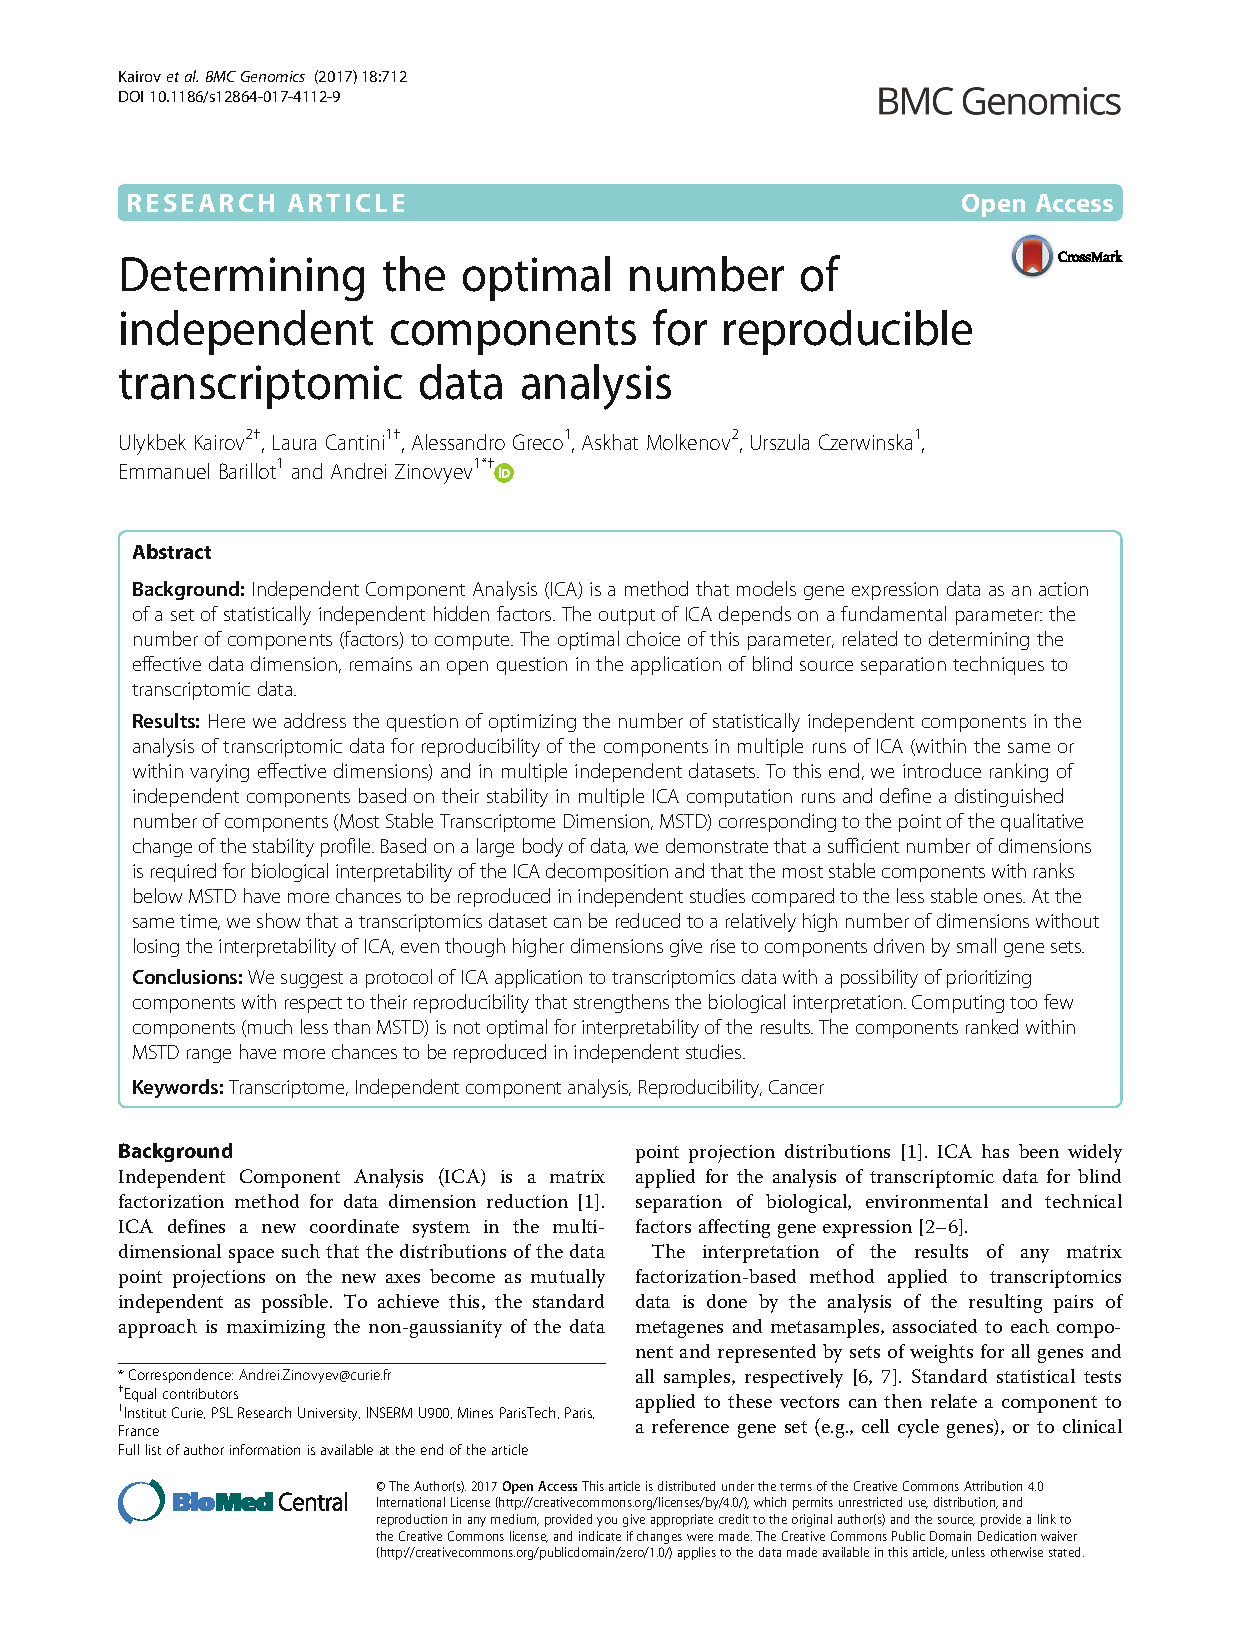
\includepdf[pages={1-}, scale=1]{pdf-ext/BMCMSTD.pdf}

\hypertarget{lva}{%
\chapter{Application of Independent Component Analysis to Tumor
Transcriptomes Reveals Specific and Reproducible Immune-Related
Signals}\label{lva}}

\chaptermark{Reproductibility if ICA: Breast cancer}

\textbf{Urszula Czerwinska}, Laura Cantini, Ulykbek Kairov, Emmanuel
Barillot, Andrei Zinovyev

\emph{Published in
~\href{https://link.springer.com/bookseries/558}{Lecture Notes in
Computer Science}~book series (LNCS, volume 10891) at conference LVA/ICA
2018:~\href{https://link.springer.com/book/10.1007/978-3-319-93764-9}{Latent
Variable Analysis and Signal Separation}, 6 June 2018}

\hypertarget{context-1}{%
\section{Context}\label{context-1}}

LVA/ICA conference is an interdisciplinary conference that gathers
researches working on Latent Variable Analysis and Signal Separation in
different fields of application. Works presented at LVA/ICA conference
can be both methodological and application works. Submitted papers are
reviewed by at least three members of the Technical Program Committee
(TPC) or by competent additional reviewers assigned by the TPC members.

I have decided to expose my work on immune-related signals obtained
using the fastICA algorithm to the signal deconvolution community in
order to receive feedback from the experts of the field. It was a great
chance to systematize my findings on overdecomposition of breast cancer
transcriptomes and describe them in details. I did not aim to expand
biological interpretation in this work given the technical character of
the conference.

\hypertarget{description-1}{%
\section{Description}\label{description-1}}

In this work, I applied ICA to six breast cancer datasets in a way to
obtain a high number of sources (\(k \gg MSTD\) as described in the
previous chapter). Then, I identified the sources related to the immune
signals in all of the datasets. Finally, I concluded that three
cell-types could be identified: T-cell, B-cell and Myeloid cells in most
of the datasets.

I am using the protocol of decomposition defined in the previous
chapter:

\begin{enumerate}
\def\labelenumi{\arabic{enumi}.}
\tightlist
\item
  Compute the MSTD for each dataset
\item
  If number of samples is \textgreater{}100 then decompose to \(k\)=
  100, otherwise to the maximal possible number of components (\(k\) =
  \(m\)) (assuming that 100 \(\gg\) 25 - the average MSTD)
\item
  Interpret the components with the gene enrichment methods
\end{enumerate}

I also improved this over-mentioned protocol with additional steps that
will be later included in
\href{https://urszulaczerwinska.github.io/DeconICA/}{DeconICA R package}
described in \protect\hyperlink{deconica}{chapter 6}.

\begin{enumerate}
\def\labelenumi{\arabic{enumi}.}
\item
  The components of the \(S\) matrix are oriented in the direction of
  the \emph{heavy tail} (the side of an ICA component with absolute
  higher weights) so that the \emph{top} genes are always at the
  positive side.
\item
  The components are interpreted through correlations with two panels:

  \begin{itemize}
  \tightlist
  \item
    reference metagenes, published in \citep{Biton2014} - the factors
    present in most tumor transcriptomes
  \item
    immune cell-type signatures used by CIBERSORT \citep{Newman2015} as
    pure cell-type profiles
  \item
    reciprocity was a condition to label the components with reference
    metagenes and maximal correlation for immune cell-type signatures
  \end{itemize}
\end{enumerate}

\hypertarget{impact-on-the-further-work-1}{%
\section{Impact on the further
work}\label{impact-on-the-further-work-1}}

With six independent datasets, I validated the hypothesis that using
decompositions of \(k \gg MSTD\). It is possible to compute signals
corresponding to immune cell types in tumor transcriptomes.

I was also able to test different ways to characterize components and
chose the one giving the most consistent results in many datasets. This
work was an important step that enabled me to develop an R package and
apply it to over 100 cancer datasets.

In the next chapter, I will show a comparison of this approach with an
alternative method: Nonnegative Matrix Factorisation (NMF).

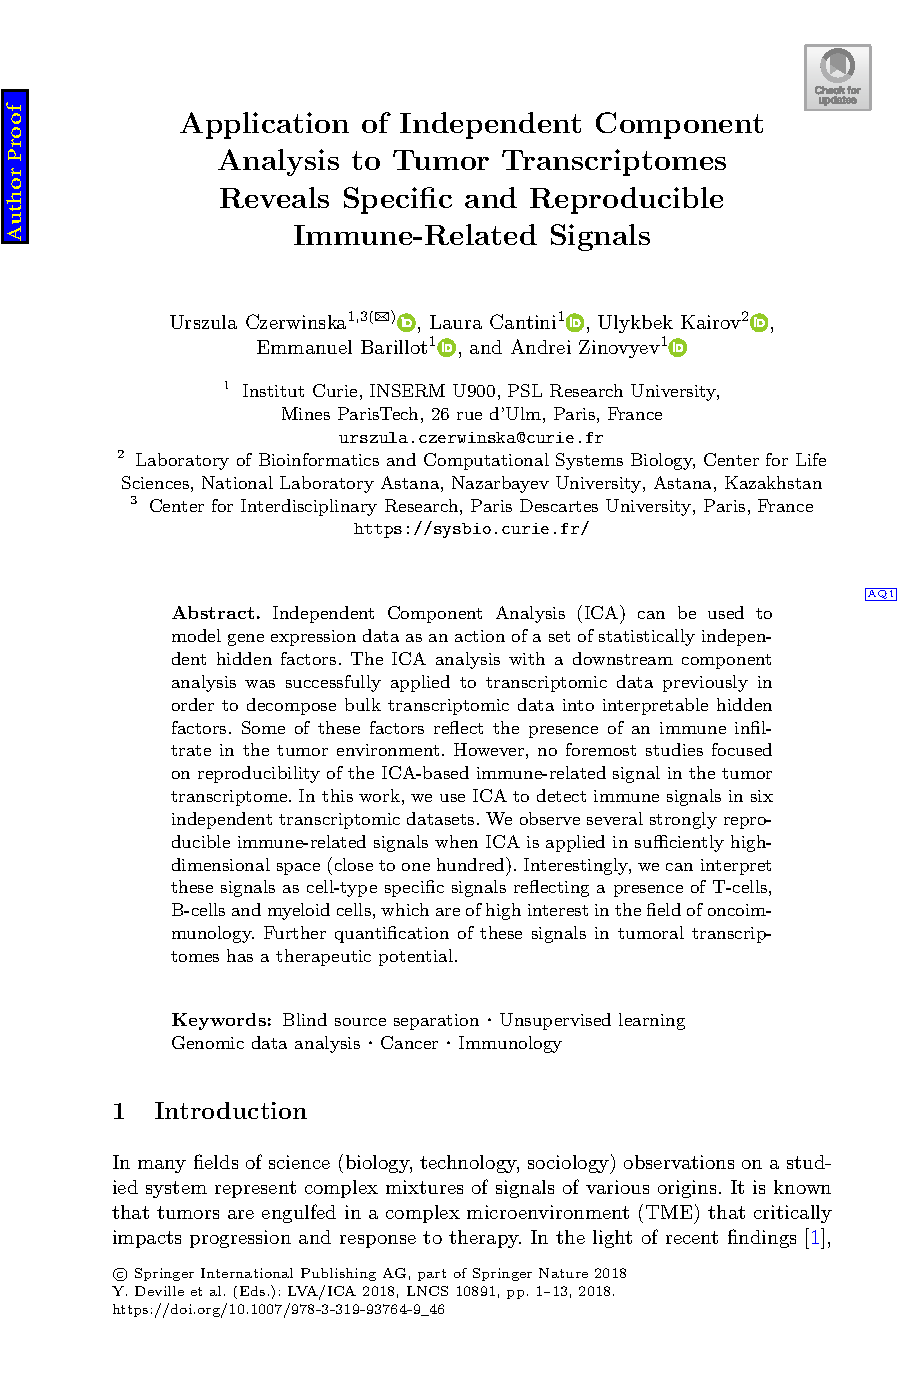
\includepdf[pages={1-}, scale=1]{pdf-ext/LVAICA_proof.pdf}

\hypertarget{nmfica}{%
\chapter{Comparison of reproducibility between NMF and
ICA}\label{nmfica}}

\chaptermark{Reproducibility: NMF vs. ICA}

NMF and ICA are algorithms often applied to solve blind source
deconvolution problem. NMF gained popularity as a tool of transcriptomic
analysis reflected in many publications
\citep{Moffitt2015, Shen-Orr2013, Brunet2004, Repsilber2010}. However,
none of these works compare components obtained from different datasets
between each other.

The non-negativity constraint, an attractive concept in the case of
non-negative transcriptome counts, may be a reason why the results of
NMF decomposition are not the best candidate for our deconvolution task.
I performed an analysis that demonstrates that NMF-based metagenes are
less reproducible between different transcriptomic datasets than
ICA-based metagenes.

\hypertarget{comparing-metagenes-obtained-with-nmf-versus-ica}{%
\section{Comparing metagenes obtained with NMF versus
ICA}\label{comparing-metagenes-obtained-with-nmf-versus-ica}}

I compared the reproducibility of NMF (classical \emph{brunet} version,
see Section 2.3.6.2) and ICA (fastICA) through decomposition of four
breast cancer datasets (BRCATCGA, METABRIC, BEK,
WAN)\citep[\citet{Wang2005}]{Cancer2012, Curtis2012, Bekhouche2011}.
Those datasets were selected because of their size (number of samples
\textgreater{} 50) and because they were available in not centered
format necessary for NMF.

For NMF the procedure was following:

\begin{enumerate}
\def\labelenumi{\arabic{enumi}.}
\tightlist
\item
  data was transformed into log2(x +1)
\item
  zero-rows were removed
\item
  the algorithm assessing cophenetic index was applied to select the
  optimal number of components
\item
  datasets were decomposed with Matlab NMF implementation from
  \citet{Brunet2004} into (i) number of components suggested by the
  cophenetic coefficient (ii) MSTD dimension (iii) 50 components
  (approaching overdecomposition)
\item
  the obtained metagenes were decorrelated from the mean using a linear
  regression model
\end{enumerate}

For ICA, the procedure was following:

\begin{enumerate}
\def\labelenumi{\arabic{enumi}.}
\tightlist
\item
  data were transformed into log2(x +1)
\item
  transformed data were mean-centered by gene
\item
  our implementation of MSTD (most stable transcriptomic dimension) from
  \citep{Kairov2017} was used to evaluate most stable dimension
\item
  datasets were decomposed into (i) MSTD dimension and (ii) 50
  components (approaching overdecomposition) with Matlab implementation
  of fastICA with icasso stabilization
\end{enumerate}

I did not decompose ICA into a low number of components as we consider
it as strong underdecomposition and we suspect signals would not be the
most reproducible.

To define the optimal number of factors for NMF (\(k\)), I followed the
strategy employed in \citep{Brunet2004} using the cophenetic coefficient
which is a metric related to the stability of clusters obtained over
iterative runs of NMF.

\begin{quote}
\emph{{[}\textbf{The cophenetic coefficient}{]} is defined as the
Pearson correlation between the samples' distances induced by the
consensus matrix (seen as a similarity matrix) and their cophenetic
distances from a hierarchical clustering based on these very distances
(by default an average linkage is used)} \citep{Brunet2004}
\end{quote}

\emph{The cophenetic distance} between two observations that have been
clustered is defined to be the intergroup dissimilarity at which the two
observations are first combined into a single cluster. The minimum of
the cophenetic coefficient values over \(k\) indicates the optimal
number of factors.

Finding the best \(k\) number of factors for NMF of the biggest dataset
(METABRIC) for \(k\) ranging from 2 to 50 took 30245 minutes (3 weeks).
Therefore, I limited the \(k_{max}\) to 50 components (maximal number of
factors) and not to 100 as initially planned.

Once, the four datasets were decomposed to MSTD, Cophenetic\(_{min}\)
and 50, I proceed to the comparison of the components between datasets.
I correlated all obtained metagenes with each other and with known
reference metagenes \citep{Biton2014}. We represented the results in the
form of a correlation graph where nodes are metagenes from different
datasets and decomposition levels, and edge width corresponds Pearson
correlation coefficients (Fig \ref{fig:icavsnmf}).

\begin{figure}

{\centering 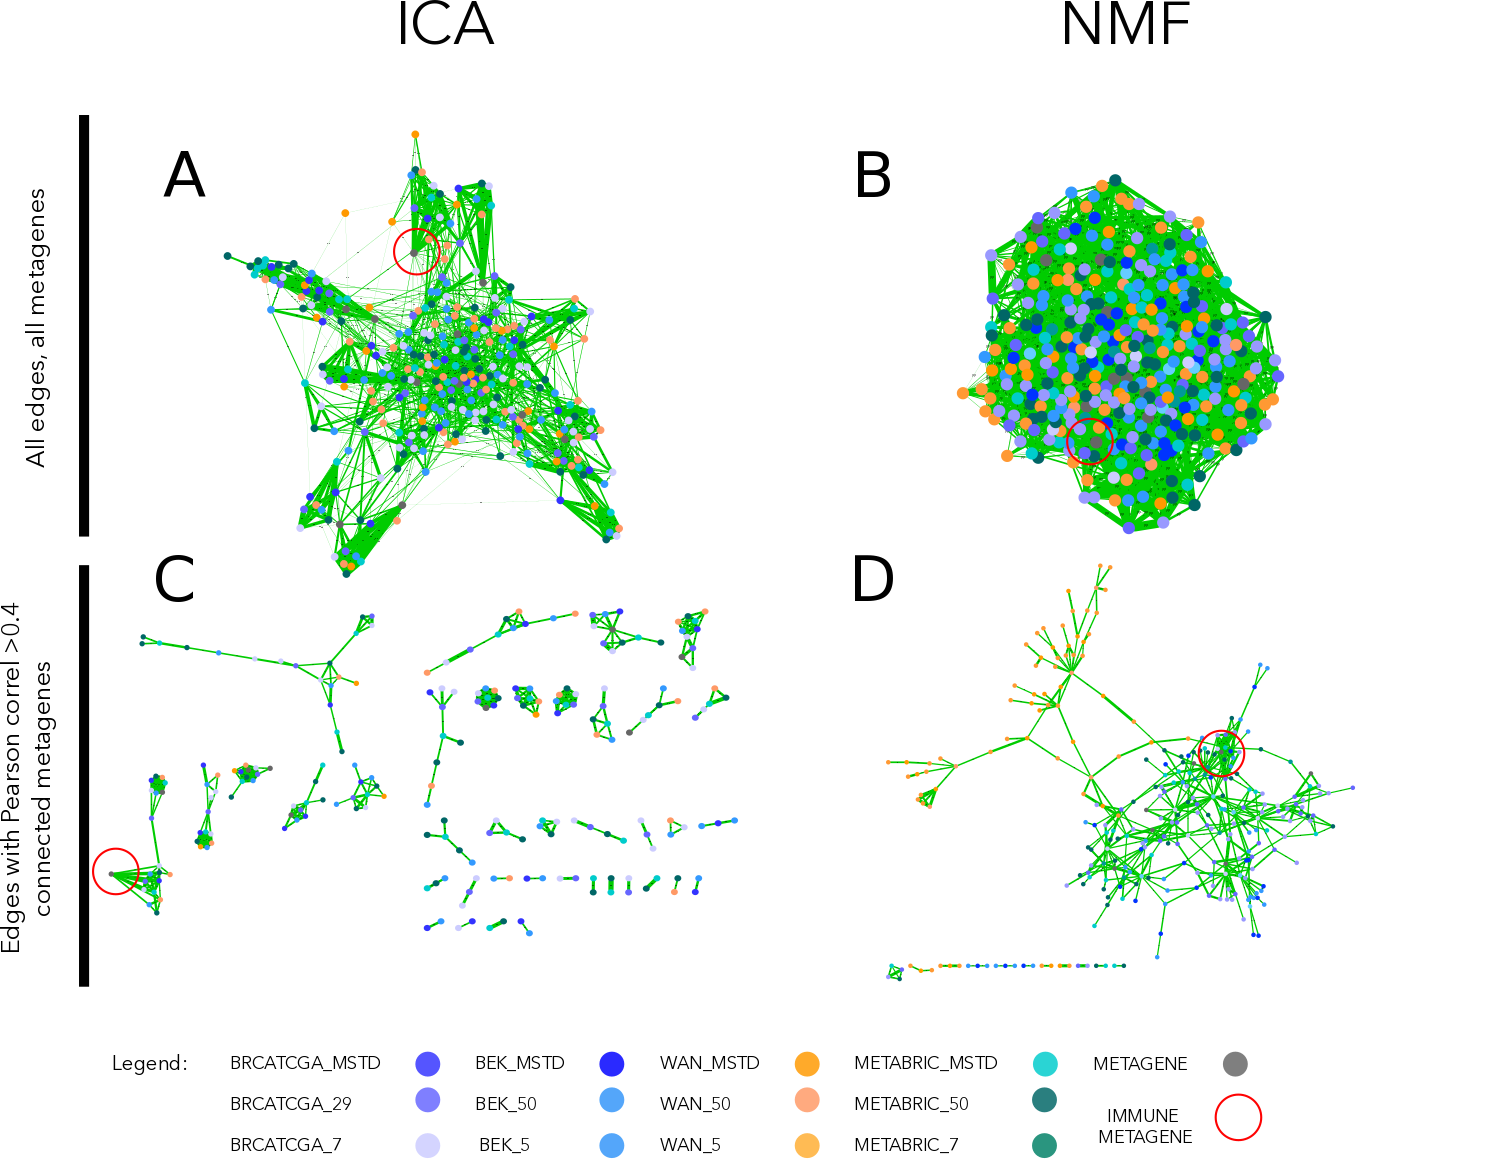
\includegraphics[width=1\linewidth]{figures-ext/ICANMF} 

}

\caption[Correlation graph of ICA and NMF multiple decompositions]{\textbf{Correlation graph of ICA and NMF multiple
decompositions.} In the upper part of the figure (A, B) we observe the
correlation graph of all metagenes (ICA or NMF-based) displayed using
edge-weighted bio layout. In the lower part of the figure (C, D) we
applied \textgreater{}0.4 thresholds to filter the edges. In the case of
ICA (C), remaining nodes form pseudo-cliques, immune-related
pseudo-clique is highlighted. In the case of NMF (D), components cluster
by the dataset. Edges' width corresponds to Pearson correlation
coefficient. Node colors correspond to the dataset from which a metagene
was obtained (see legend).}\label{fig:icavsnmf}
\end{figure}












I expected to observe a subset of components from different datasets (no
matter the decomposition level) correlated with each other firmly and
much less with other components in order to confirm that the signal is
reproducible (can be found in several dataset) and specific (can be
matched to one corresponding signal in another dataset). I used the
reference components here to help with the identification of signals
(labeling) of indicative nature. In ICA-based correlation of components,
without applying any threshold (Fig \ref{fig:icavsnmf}A), some emerging
clusters can be remarked and after application of \textgreater{}0.4
thresholds on the Pearson correlation coefficient value(Fig
\ref{fig:icavsnmf}C) numerous pseudo-cliques emerge. While for metagenes
from NMF decomposition, they are more tightly connected globally and
when the threshold is applied components group by the dataset. In NMF
decomposition, if it is hard to define different signals as the
components seem all related to each other. We can see from (Fig
\ref{fig:icavsnmf}D) that the IMMUNE signal is correlated
\textgreater{}0.4 with a high number of NMF components that are also
linked to some other components. In ICA (Fig \ref{fig:icavsnmf}C)
components related to the IMMUNE metagenes form a pseudo-clique that is
related only with one link to INTERFERON metagene. This makes them much
more specific, and therefore the interpretation is more straightforward.

\hypertarget{summary-3}{%
\section{Summary}\label{summary-3}}

This simple analysis illustrates that NMF applied to cancer
transcriptomes decomposes them to metagenes that are not selectively and
specifically matching between datasets. In part, this is because NMF
components are correlated with the average gene expression. Therefore,
NMF can be sensitive to the normalization. However, even after the
``removal'' through linear regression, this phenomen persist. It is not
clear why, from a mathematical perspective, we observe such a
discrepancy of interpretation of NMF and ICA components.

It is also possible that using a different method to find correct
decomposition dimension (\(k\)) should be used. Ideally, different NMF
implementation should be tested to verify if using different error
updates can have an impact on the results.

In practice, it will not always be possible to work with the data
processed in the same way. Using ICA for decomposition seems to be more
straightforward, and the obtained components are easier to interpret as
biological functions (thanks to the reciprocal matching) without a need
to renormalize datasets.

A deepened extension of this study was performed by \citet{Cantini2018}
and is available online.

\hypertarget{deconica}{%
\chapter{DeconICA: an R package for Deconvolution of omic data through
Immune Components Analysis}\label{deconica}}

\chaptermark{DeconICA R package}

\emph{Selected content from this chapter is a part of a publication in
preparation}

\hypertarget{from-blind-deconvolution-to-cell-type-quantification-general-overview}{%
\section{From blind deconvolution to cell-type quantification: general
overview}\label{from-blind-deconvolution-to-cell-type-quantification-general-overview}}

In the introduction chapters 1 and 2, I have presented why there is a
need to extract knowledge about the immune system from the cancer
transcriptomes and how it can be done. In the result chapters 3, 4 and 5
I have presented studies of ICA application to transcriptomes, ideas for
finding a way to extract the cell-specific components through
\emph{overdecomposition} procedure.

However, I in the presented works, the proposed biological
interpretation was not deepened. In order to enable standardized
unsupervised deconvolution framework and an interpretation of obtained
components as immune cell types and their quantification that is
scalable, I introduce, in this chapter, a method named ``DeconICA'':
\textbf{Decon}volution of omic data through \textbf{I}mmune
\textbf{C}omponents \textbf{A}nalysis. The method is published online on
GitHub:
\href{https://github.com/UrszulaCzerwinska/DeconICA}{UrszulaCzerwinska/DeconICA}
in the form of an R package and has a
\href{https://zenodo.org/record/1250070}{doi number
(10.5281/zenodo.1250069)} for citations. In this chapter, I will
describe my pipeline and the rationale behind my strategy of analysis
and quantification of components. I will also briefly compare its
performance in the quantifying abundance with previously published
methods. The user guide for DeconICA R package is available in
\protect\hyperlink{deconicatut}{Annexes} and online at
\url{https://urszulaczerwinska.github.io/DeconICA/DeconICA_introduction.html}.

\hypertarget{unsupervised-deconvolution}{%
\section{Unsupervised deconvolution}\label{unsupervised-deconvolution}}

So far, I have focused on ICA-based decompositions of transcriptomes. In
the \protect\hyperlink{nmfica}{chapter 5}, I have compared ICA and NMF
decompositions concluding that ICA-based decompositions shall be more
convenient. In my work, because of my team expertise, the proven
computational efficiency, interpretability, and reproducibility, I will
use mostly ICA components to deconvolve tumor data (analysis described
in the next \protect\hyperlink{results}{chapter 6}). However, the
constructed interpretation pipeline can take as input any metagenes,
i.e., NMF factors, convex-hull derived sources or attractor metagenes
(methods described in \protect\hyperlink{methods}{chapter 2}).

In this section, I will explain the DeconICA pipeline (Fig.
\ref{fig:deconicaschema}) based on the stabilized fastICA
overdecomposition protocol as it is resulting from our expertise and
results are satisfying.

\begin{figure}

{\centering 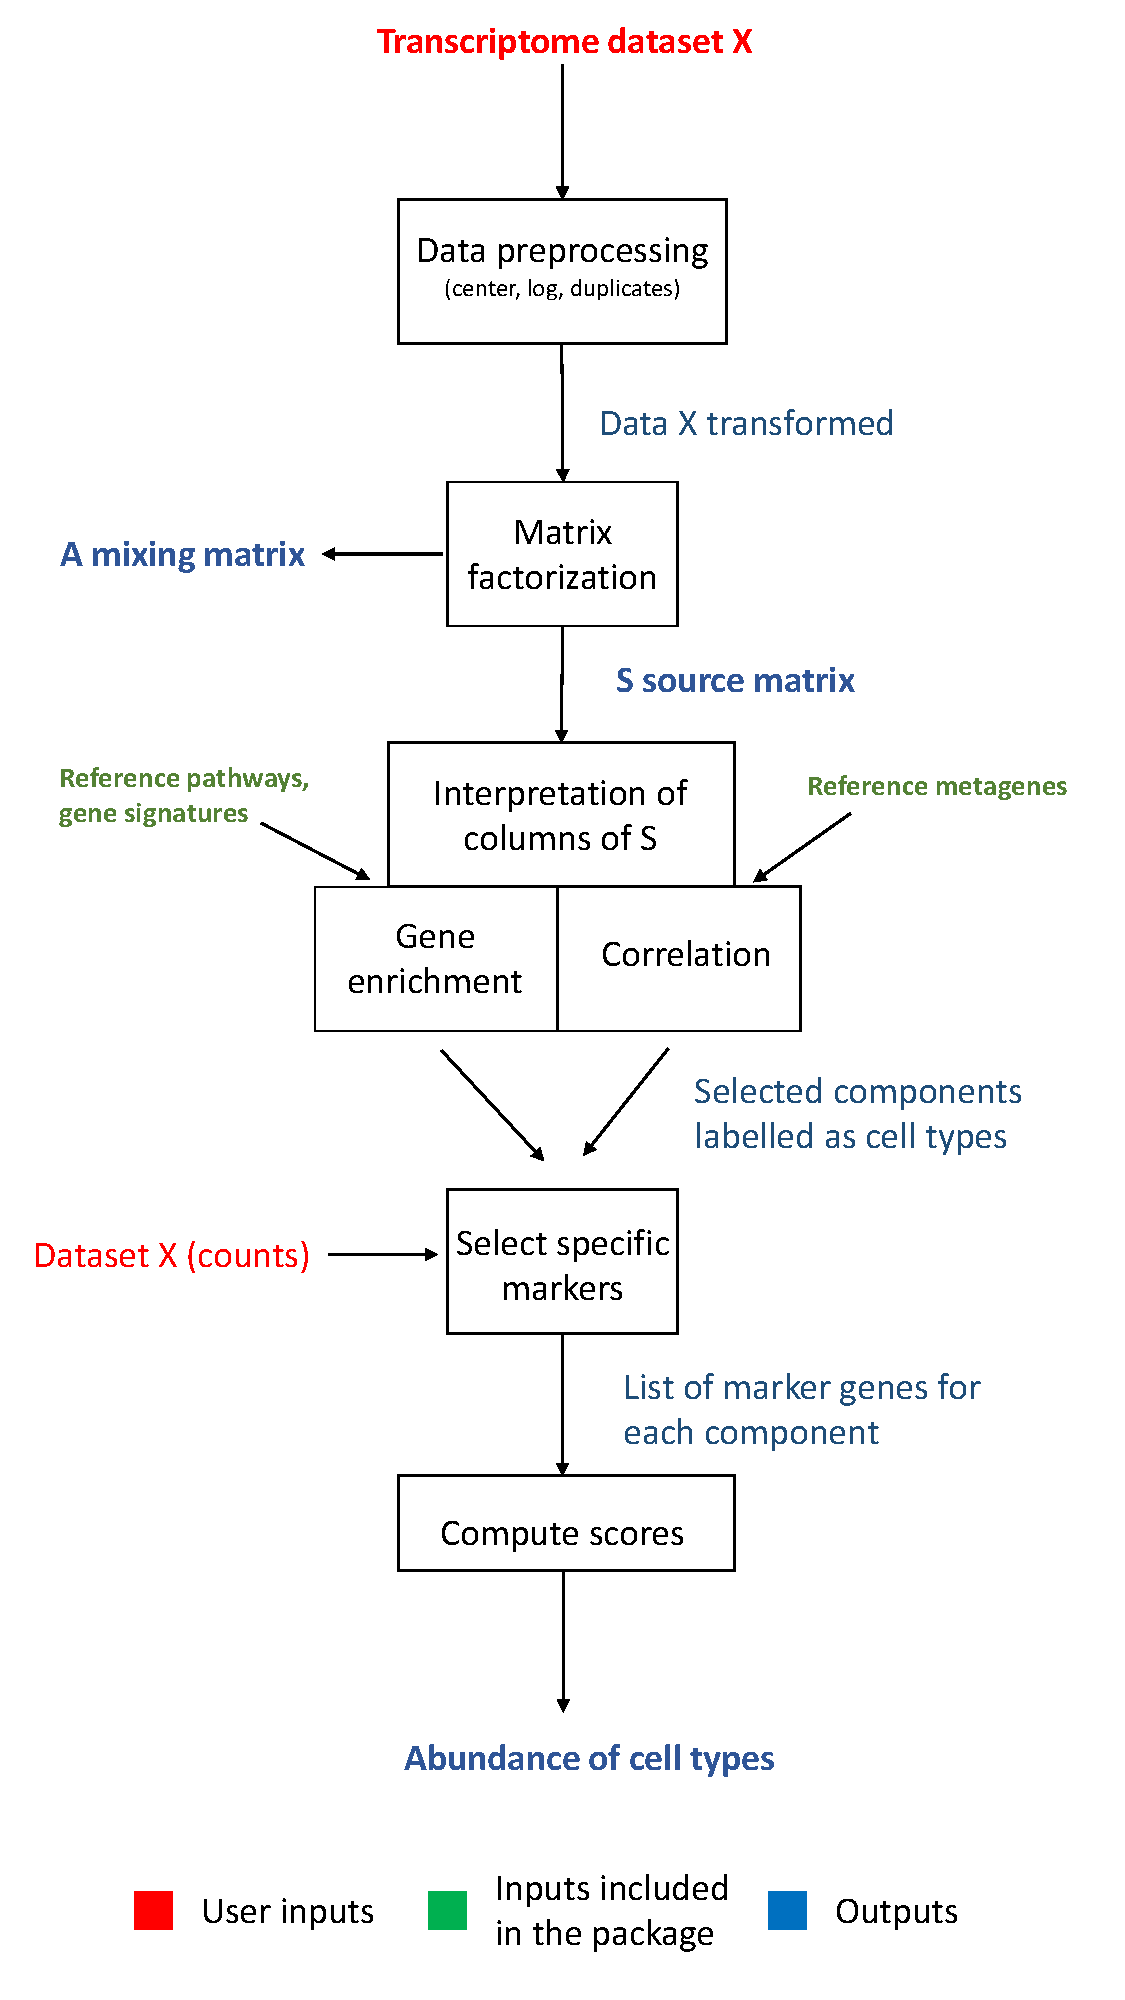
\includegraphics[height=0.8\textheight]{figures-ext/deconica_schema} 

}

\caption[Flowchart of DeconICA method]{\textbf{Flowchart of DeconICA method}. In
this flowchart steps of DeconICA are represented as boxes. Each
operation corresponds to one or multiple functions in the R package.
Input data X (red) is preprocessed and then decomposed into components.
Interpretation of the components is performed with correlation or gene
enrichment analysis (using reference materials - green). For components
labeled as cell types or other important factors, abundance can be
estimated using top genes of each component and computing average of
counts in a non-log scale of those genes. Main outputs are ( in blue),
the S component matrix, labeled components, and their abundance scores.}\label{fig:deconicaschema}
\end{figure}












\hypertarget{fastica-overdecomposition-protocol}{%
\subsection{FastICA overdecomposition
protocol}\label{fastica-overdecomposition-protocol}}

The main inputs of unsupervised deconvolution methods are data matrix
\(X\) and number of output sources \(k\). I have developed a protocol
that can define \(k\) for fastICA algorithm applied to cancer
transcriptome datasets and prepares the data for interpretation steps.

\hypertarget{data-transformation}{%
\subsubsection{Data transformation}\label{data-transformation}}

The input matrix of gene expression is transformed to \(log_{2}(x +1)\)
where is \(x\) is a data point and then row (gene) centered: mean of
each row is removed. This step is necessary for ICA algorithm.

If gene names or probes are provided, the duplicated genes are removed -
the genes with higher variance are kept.

\hypertarget{determining-k-number-of-sources}{%
\subsubsection{\texorpdfstring{Determining \(k\) number of
sources}{Determining k number of sources}}\label{determining-k-number-of-sources}}

If the number of sources in the mixture is known, \(k\) can be fixed by
the user.

In case of complex mixtures of tumor transcriptomes, the input matrix of
gene in rows (\(n\)) and samples (\(m\)) in columns is decomposed into
\(k=100\) components if \(m\) \textgreater{} 100. If m
\textless{}\(100\), then the \(k\) number is equal to the number of PCA
components necessary to explain 90\% of data.

If a different data type is analyzed, one can also compute MSTD (see
\protect\hyperlink{mstd}{chapter 3}) of the data and redefine the
\emph{overdecompositon} dimension.

\hypertarget{fastica}{%
\subsubsection{FastICA}\label{fastica}}

The fastICA algorithm uses icasso stabilization (described in chapter 2
section 2.3.6.3) to obtain an average representation of components over
the \(i\) number of iterations (by default \(i=100\)) in order to buffer
the effect of local minima resulting from stochastic initializations.

The stabilized version of FastICA algorithm is, so far, only available
in Matlab. A custom Matlab scripts ``fastica++'' that I am using have
initially been distributed with
\href{https://github.com/LabBandSB/BIODICA}{BIODICA software} by
Zinovyev and Kairov. I have created an R interface to use it easily
without any knowledge of Matlab. I also provided a detailed description
on how and why use this version of fastICA as a part of
\href{https://urszulaczerwinska.github.io/DeconICA/Icasso.html}{DeconICA
tutorial} (available in Annex Z), even without Matlab software installed
(through a Docker image). Although it is possible to use non-stabilized
and slower R version of fastICA, it impacts the results significantly.

To remind, the input \(X_{n\times m}\) matrix is in therefore decomposed
to \(S_{k\times n}\) source matrix and \(A_{m \times k}\) mixing matrix,
where \(k\) is the number of components. Therefore, for example, having
as an input transcriptome matrix of 20 000 genes and 150 samples, if
\(k\) = 100 (overdecomposition), then the \(S\) will have dimensions 20
000 \(\times\) 100 and \(A\) matrix 100 \(\times\) 150.

\hypertarget{orienting-the-components}{%
\subsubsection{Orienting the
components}\label{orienting-the-components}}

The \(S\) columns (components/sources) contain positive and negative
values that the projections of data in the given dimension. The sign
(positive or negative) cannot be directly interpreted. Therefore the
values should be seen as an absolute value of the projection. The genes
ranked top (by the absolute value), separately for positive and negative
ends) are representative for the component. Usually, only one end leads
to a biological interpretation. To define which end should be
interpreted, I apply a simple statistical procedure (Fig.
\ref{fig:orienting}).

I plot density distribution of a component, compute a standard deviation
and count how many genes are above or below a threshold of \(t\). I
define \(t =\) 3 standard deviation (sd). If there are no points
\textgreater{}\(t\), the threshold is lowered to 2sd, etc. The end of
the independent components with a higher number of genes over the
threshold is decided to be the one representing the component that we
call \emph{heavy tail}.

If the \emph{heavy tail} is negative the component weights are
multiplied by -1 in order to reverse signs.

In this way, all the representative ends of \(S\) are all positive which
makes the further steps easier.

This procedure can fail if the initial sources are coming from, i.e.,
uniform distribution and the component \(S_i\) is symmetric. In those
cases, components can be oriented for examples based on correlation with
known sources (to have only positive correlations). In practical terms,
there is an option to skip this step.

Generally, the orientation procedure applies to microarray and RNA-seq
transcriptomes that are overdecomposed.

\begin{figure}

{\centering 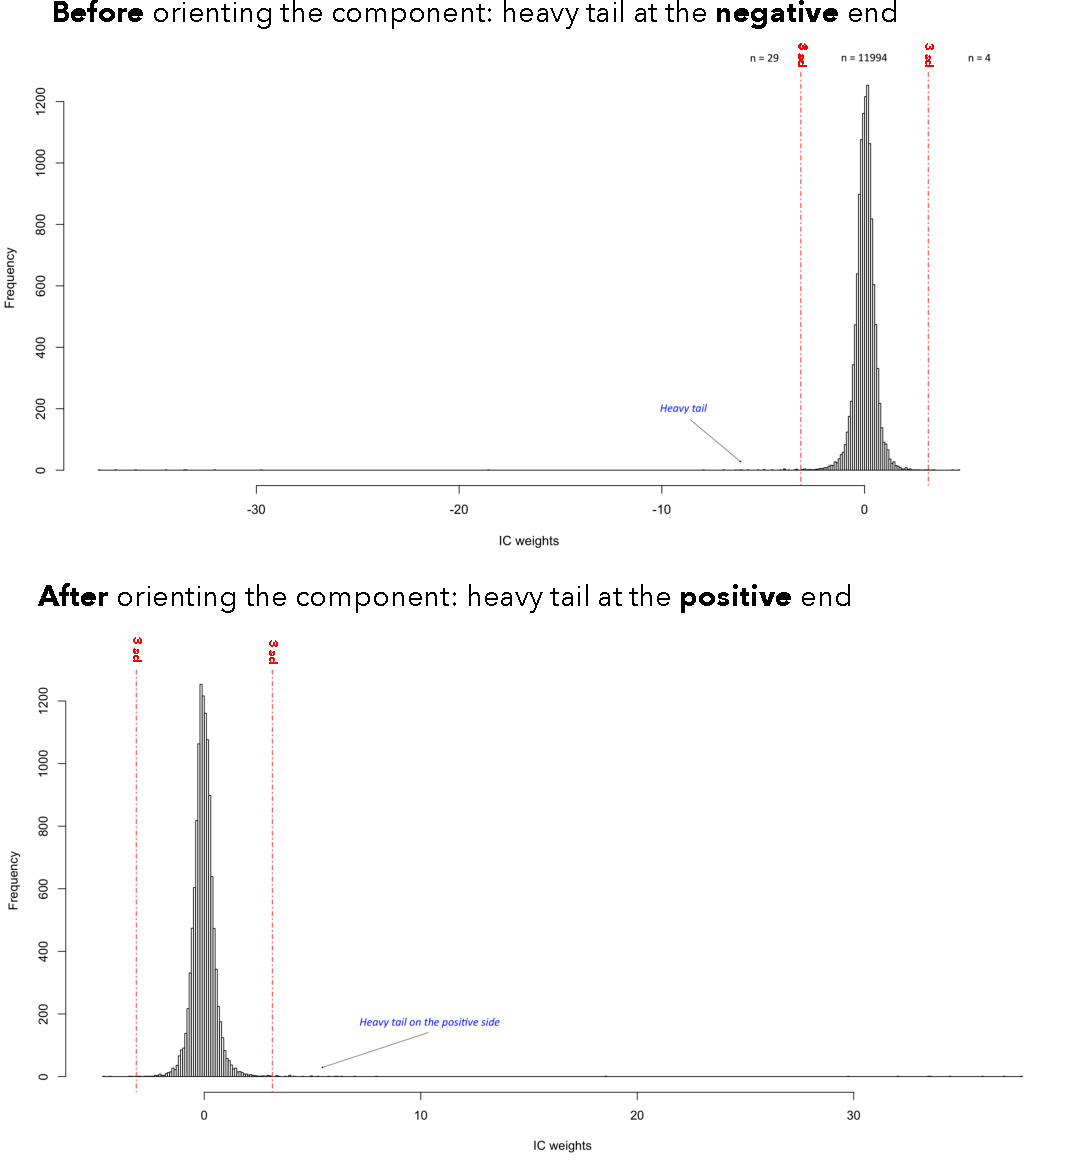
\includegraphics[width=0.7\linewidth]{figures-ext/orienting} 

}

\caption[Principle of components orienting]{\textbf{Principle of components orienting}. An
independent component illustrated here has more values under the
threshold of - 3 standard deviations (sd) than over 3 sd (64 vs.~4).
Therefore the heavy tail is on the negative side. DeconICA orients the
heavy tail towards the positive side. This procedure is applied to all
independent components.}\label{fig:orienting}
\end{figure}








\hypertarget{interpretation-of-the-components}{%
\section{Interpretation of the
components}\label{interpretation-of-the-components}}

\hypertarget{identification-of-immune-cell-types-with-an-enrichment-test}{%
\subsubsection{Identification of immune cell types with an enrichment
test}\label{identification-of-immune-cell-types-with-an-enrichment-test}}

Based on previous work of our team, a way to characterize obtained
components is to select top genes and verify if they belong to a
described biological pathway or a list of genes. There is a wide choice
of websites (i.e., \href{http://biogps.org/\#goto=welcome}{BioGPS},
\href{https://toppgene.cchmc.org/}{Toppgene} or
\href{http://amp.pharm.mssm.edu/Enrichr/}{EnrichR}) that compares a
selected list of genes with databases and computes, in different ways,
an enrichment score. Often, proposed pathways or conditions are quite
general, for instance, type of immune response and associated cell type
would not be specified. Another way to compute enrichment is to use GSEA
(described in section 2.3.3). It is possible that I will extend the
package to facilitate an enrichment with GSEA (for example using the
\emph{fgsea} R package \citep{Sergushichev2016}). However, the essence
of the interpretation though enrichment is not the score itself but the
pathways/processes identified to be associated with the analyzed
component.

This is why, in DeconICA package, I implemented a simple Fisher exact
test (described in section 2.3.3) that computes a significance of an
overlap between a list of top genes from a component and a collection of
known gene sets. An ensemble of known pathways is called the universe.

I set some default parameters for the analysis: the number of top genes,
minimal and maximal length of the gene list in the universe, p-value
correction. I have tested the enrichment of the components in a custom
collection of cell-type specific signatures published in primary
research articles or as a part of deconvolution tools.

Enrichment allows to link a list of component's top genes to biological
process, but the p-value depends strongly on the size of the universe
and the size of gene sets. In most cases, only a small number of genes
is known to be specific to a cell type. These specific genes are not
always expressed in the analyzed dataset. Therefore, often false
positives are found only due to technical dimension of the analysis.
Depending on which compendium of signatures I used I would identify very
different cell types with the enrichment test for the same component.

The enrichment methods were not conceived for small and close related
gene sets. A more sophisticated solution like in xCell \citep{Aran2017},
are necessary to overcome those limitations. Thus, I would advise using
basic enrichment for exploratory analysis of the general factors
impacting the transcriptome rather than to identify cell types.

Looking for more robust evaluation of immune cells identification I have
proposed a correlation-based interpretation.

\hypertarget{correlation-based-identification}{%
\subsubsection{Correlation based
identification}\label{correlation-based-identification}}

\hypertarget{reciprocal-match}{%
\subsubsection{Reciprocal match}\label{reciprocal-match}}

Working with many datasets, I remarked that correlation with a reference
metagene enables quickly and robustly label the components. The
reference metagenes provided with DeconICA were published in the study
of \citet{Biton2014}. As these signals represent independent biological
factors, one reference metagene should match one component. This is why
I applied the rule of reciprocal matching to label components
corresponding to reference metagenes.

Formally, the reciprocity rule is defined as follows. Given correlations
between the set of reference metagenes \(M=\{M_{1},...,M_{m}\}\) and
\(S\) source matrix \(S=\{IC_{1},...,IC_{N}\}\), if
\(S_{i}=argmax_k (corr(M_{j},S_{k}))\) and
\(M_{j}=argmax_k (corr(S_{i},M_{k}))\), then \(S_{i}\) and \(M_{j}\) are
reciprocal. This rule was already applied previous publications of our
group \citep{Kairov2017, Czerwinska2018, Cantini2018}. An important
feature of this association is that it is not based on the strength of
the correlation and hypothesise that even weak correlation can be
meaningful if there is an exclusive reciprocal match between reference
metagene and a component.

\hypertarget{maximal-correlation-match}{%
\subsubsection{Maximal correlation
match}\label{maximal-correlation-match}}

As there are no established metagenes of immune cells, I used a
signature matrix published in \citep{Newman2015} LM22 containing 22
immune cells profiles reduced to 510 genes that should enable the
differentiation between the cell types. I used specifically this
reference as it had more genes than other similar matrices (i.e., the
one from EPIC \citep{Racle2017} contains \(\approx\) 100 genes). The
number of genes is critical because the correlation needs to be based on
a minimal number of genes to be reliable. It may happen that genes
present in the reference profiles are not present in studied gene
matrix. Therefore, more genes in the reference set to increase the
probability to interpret the data. Generally, the power of the
correlation coefficient increases with the number of genes used to
compute it (the overlap between the reference and the analyzed data). On
the other hand, the full cell profiles (10000-20000 genes) would
introduce a significant amount of noise.

To assign a reference cell type to a component, I adopted a strategy
different from described in the previous section. It is known that cell
type subtypes have quite similar expression profiles. Therefore, the
match of one component to different subtypes of the same cell type
should not be penalized. I have also remarked that sometimes closely
related cell types cannot be discriminated and one component can be the
most related to, i.e., T-cell and NK. Thus, the label is attributed
through maximal correlation, for instance, which of all components has
the highest correlation coefficient with given reference profile.

This results in the fact that each reference metagene has a component
attributed. Then, the user needs to define manually is the association
can be trusted from the value of the Pearson correlation coefficient.
Usually, if there is one component with remarkably stronger associated
to the reference cell type than others, the association can be trusted.
A graphical representation (Fig. \ref{fig:corrEx}) can be help in
decision making. This step should be automatized if possible in the
future.

\begin{figure}

{\centering 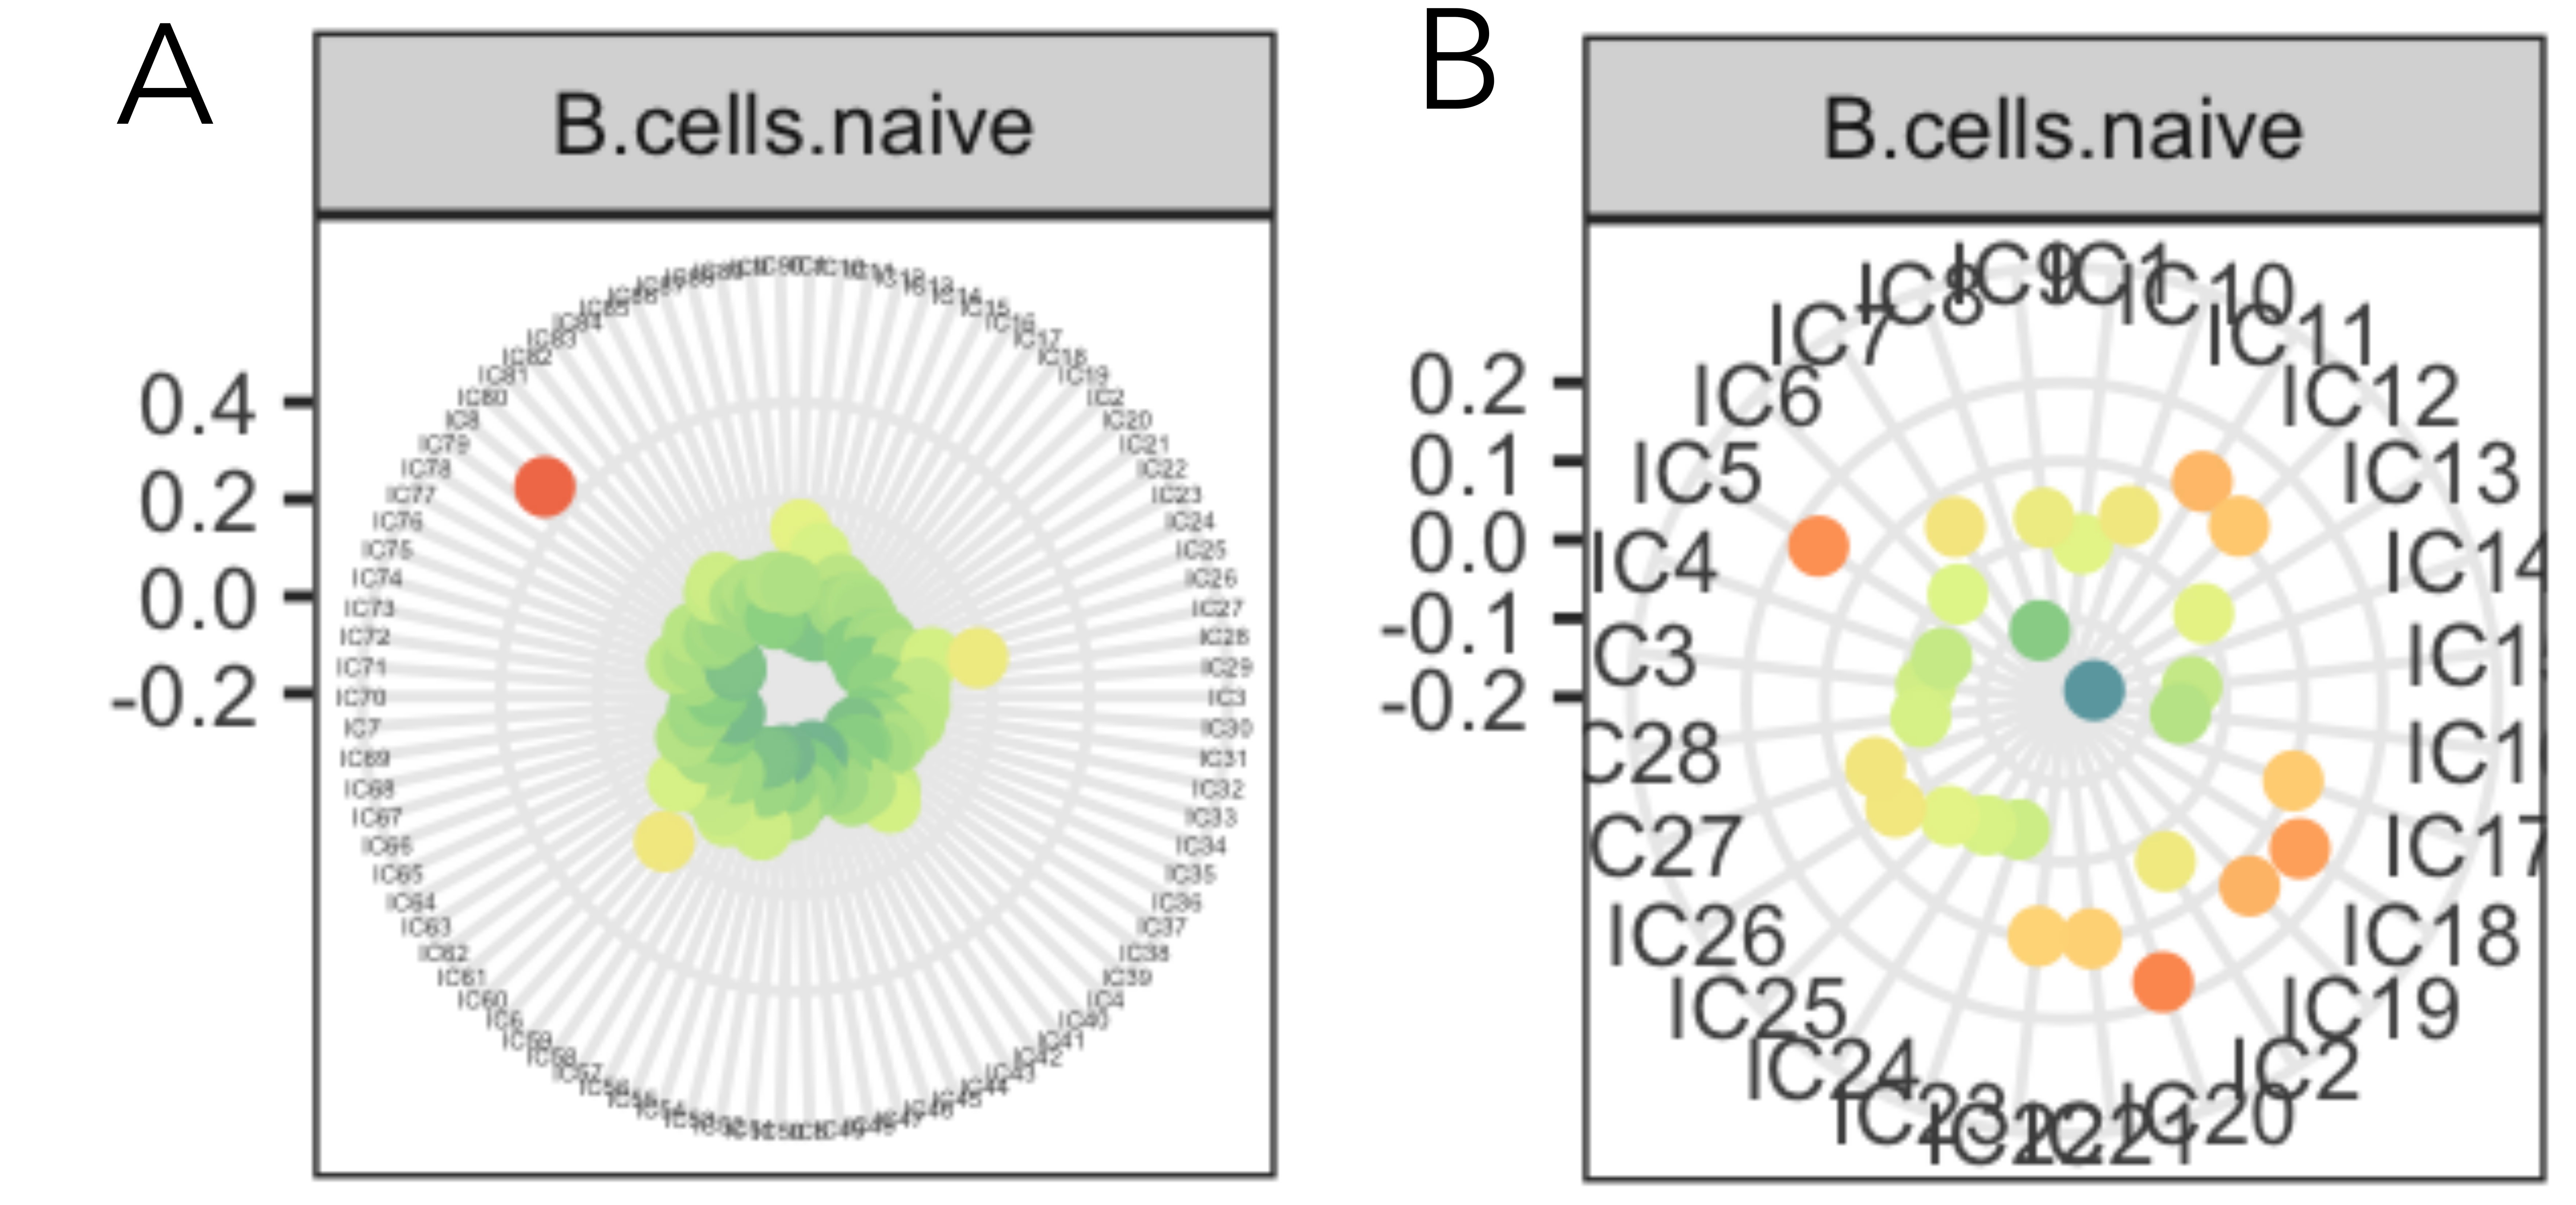
\includegraphics[width=0.7\linewidth]{figures-ext/corrEx} 

}

\caption[Example of sucesfull and unsucessful component matching to refrence]{\textbf{Example of successful and unsuccessful
component matching to a refrence}. Among all components there can be one
component that matches the reference profile (A) or many components that
weekly matches the reference profile (B). Only in the case, `A' the most
correlated component should be labeled as B-cell.}\label{fig:corrEx}
\end{figure}







\hypertarget{computing-the-abundance-of-the-identified-cell-types}{%
\section{Computing the abundance of the identified
cell-types}\label{computing-the-abundance-of-the-identified-cell-types}}

Once the components are labeled, their contribution in each sample can
be estimated. For cell type related components this contribution can be
interpreted as cell-type abundance (in arbitrary units).

Before deciding on the final way in which cell-type contribution can be
evaluated, I have tested different possibilities.

In theory, the \(A\) mixing matrix reflects contributions of each
component. However, it reflects the contribution of both positive and
negative ends of components. In my protocol, one end is selected to be
representative of a biological signal. This is why \(A\) matrix scores
do not reflect well abundance of the information on cell types.

One idea was to use the components as ``pure cell-type expression'' in a
regression model (testing different regression types: SVR, quadratic
programming, simple linear regression, lasso regression). I tested this
approach on blood transcriptome benchmark (described in more details
below). The results were acceptable, but they got outperformed by the
mean of top genes approach that is included in DeconICA.

Finally, I tested the approach inspired by \citep{Becht2016}. Selecting
the most specific genes and computing arithmetic mean of the genes in
the original counts matrix. This method is based on the hypothesis that
those particular markers are unique to one cell type. Therefore gene
expression of those genes should be proportional to the abundance of the
cell type.

\hypertarget{defining-markers}{%
\subsubsection{Defining markers}\label{defining-markers}}

In \citep{Becht2016} cell-type specific markers are defined based on
expert knowledge and validated in gene expression data. In this work,
the specific markers are generated in the unsupervised deconvolution. I
adopted a hypothesis that \(n_{top}\) genes of a labeled component is a
unique signature of this component. I defined the value of \(n_{top}\)
empirically to be in a range of 10 to 30 genes.

\hypertarget{computing-scores}{%
\subsubsection{Computing scores}\label{computing-scores}}

In order to compute the scores, a mean of the selected marker genes for
each component is computed. The user has a choice between arithmetical,
geometric, harmonic or weighted mean. So far, the arithmetic means to
seem to give the best performance on the benchmark data.

\hypertarget{validation-of-the-abundance-estimation-with-deconica}{%
\section{\texorpdfstring{Validation of the abundance estimation with
\emph{DeconICA}}{Validation of the abundance estimation with DeconICA}}\label{validation-of-the-abundance-estimation-with-deconica}}

\emph{Code used to produce the validation, and more extensive
description of each step is available as a part of the
\href{https://urszulaczerwinska.github.io/DeconICA/DeconICA_introduction.html}{online
tutorial} and in Annexe X}

\hypertarget{in-silico}{%
\subsection{\texorpdfstring{\emph{In
silico}}{In silico}}\label{in-silico}}

First, the performance of the DeconICA was tested on simulated data. I
wrote a function that produces a linear mixture of randomly generated
sources of selected distribution with known proportions and possibility
to set the number of marker genes. Here I generated ten sources drawn
from the negative binomial distribution (10000 \emph{genes}) and mix
them at known proportions, adding some noise resulting in 130 mixtures
(\emph{samples}). As the ten original sources are known, a component is
attributed to an original source through reciprocal correlation. I
demonstrate that for each original source a matching component can be
identified and using 10 top markers I estimate abundance with
correlation coefficient ranging from 0.95 to 0.99 (where 1.0 is a
perfect correlation), equal to average \(R^2\)= 0.96 (Fig
\ref{fig:insilico}).

\begin{figure}

{\centering 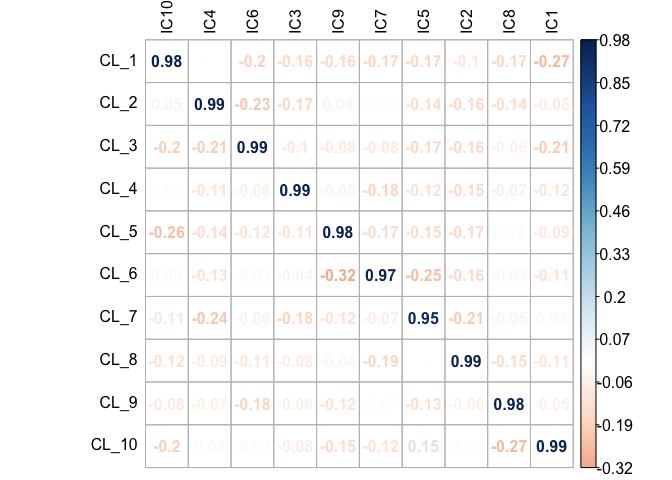
\includegraphics[width=0.7\linewidth]{figures-ext/insilico} 

}

\caption[Accuracy of estimation versus true proporitons in an in silico mixture]{\textbf{Accuracy of estimation versus true
proportions in an \emph{in silico} mixture}. The simulated matrix of
mixtures (10000 \(\times\) 130) was decomposed, and obtained components
were used to estimate proportions. The estimated proportions of each of
10 cell types were correlated with the known abundance values of the
given cell type. The Pearson correlation coefficient values are reported
in the correlation matrix.}\label{fig:insilico}
\end{figure}









\hypertarget{in-vitro}{%
\subsection{\texorpdfstring{\emph{In vitro}}{In vitro}}\label{in-vitro}}

Previously published in \citep{Becht2016} \emph{in vitro}~immune cell
types sorted from 3 healthy donors' peripheral blood and mixed at
different proportions resulting in 12 mixed samples. Following my
pipeline, data is decomposed with stabilized fastICA, each of cell types
finds its match and marker genes are defined as top 10 genes of each
component. Then the correlation with abundance is computed. The Pearson
correlation with true mixing proportions varies from 0.93 to 0.99,
average \(R^2\)= 0.94 (Fig. \ref{fig:invitro}).

\begin{figure}

{\centering 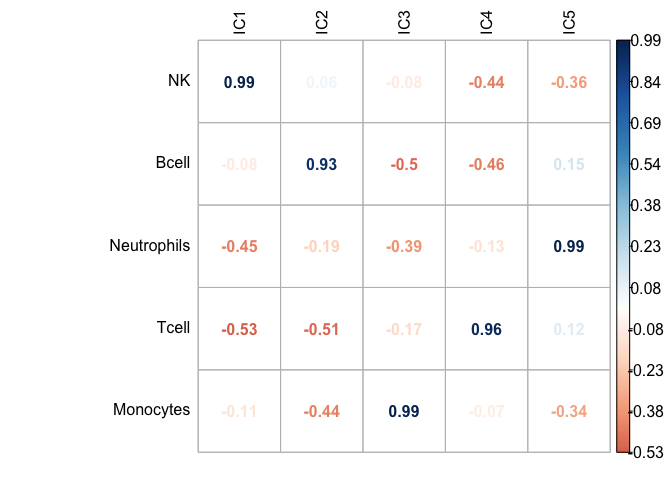
\includegraphics[width=0.7\linewidth]{figures-ext/invitro} 

}

\caption[Accuracy of estimation versus true proporitons in an in vitro mixture]{\textbf{Accuracy of estimation versus true
proportions in an \emph{in vitro} mixture}. Five different immune cell
types from three donors were mixed at known proportions. The estimated
proportions of each of 5 cell types were correlated with the known
abundance values of the given cell type. The Pearson correlation
coefficient values are reported in the correlation matrix.}\label{fig:invitro}
\end{figure}








\hypertarget{pbmc-transcriptome}{%
\subsection{PBMC transcriptome}\label{pbmc-transcriptome}}

Finally, I applied DeconICA to PBMC expression data of 104 healthy
patients, paired CyTOF proportion estimation for each sample
\citep{Whiting2015}, processed data were shared kindly by
\citep{Aran2017}. I use MSTD to estimate the optimal dimension (39).
From the correlation profiles, it can be seen that this task is
remarkably more challenging than the previous tests (Fig @(fig:radarB))
and not all cell types can be perfectly matched to components. Based on
maximal correlation a subset of components is labeled as immune cells
and based on 10 top markers abundance is computed for B-cells, T cells
CD8, T cells CD4, NK and Monocytes.

The correlation between CyTOF measured abundance and DeconICA estimated
abundance varies from 0.31 to 0.77. Some cell types as T-regs, NKT,
other T-cell, naive-B-cells subtypes could not be differentiated with
individual components. I compared DeconICA performance with five other
methods of immune cell-type deconvolution (Fig \ref{fig:comparison}).
The strategical differences between compared methods were explained in
\protect\hyperlink{methods}{Chapter 2}. All of them are recent
supervised deconvolution approaches, state-of-art at the date. DeconICA
performance is better or similar than the one of previously published
methods for the cell types that we could identify and in average has
slightly better \(R^2\).

It is necessary to mention that EPIC probably performs worse than
expected because data were not TPM normalized. For MCPcounter CD8
T-cells were matched to ``cytotoxic T-cells'' and CD4 T-cells to
T-cells. For CIBERSORT between naive B-cells and activated B-cells
better correlation was reported as ``B-cells''.

\begin{figure}

{\centering 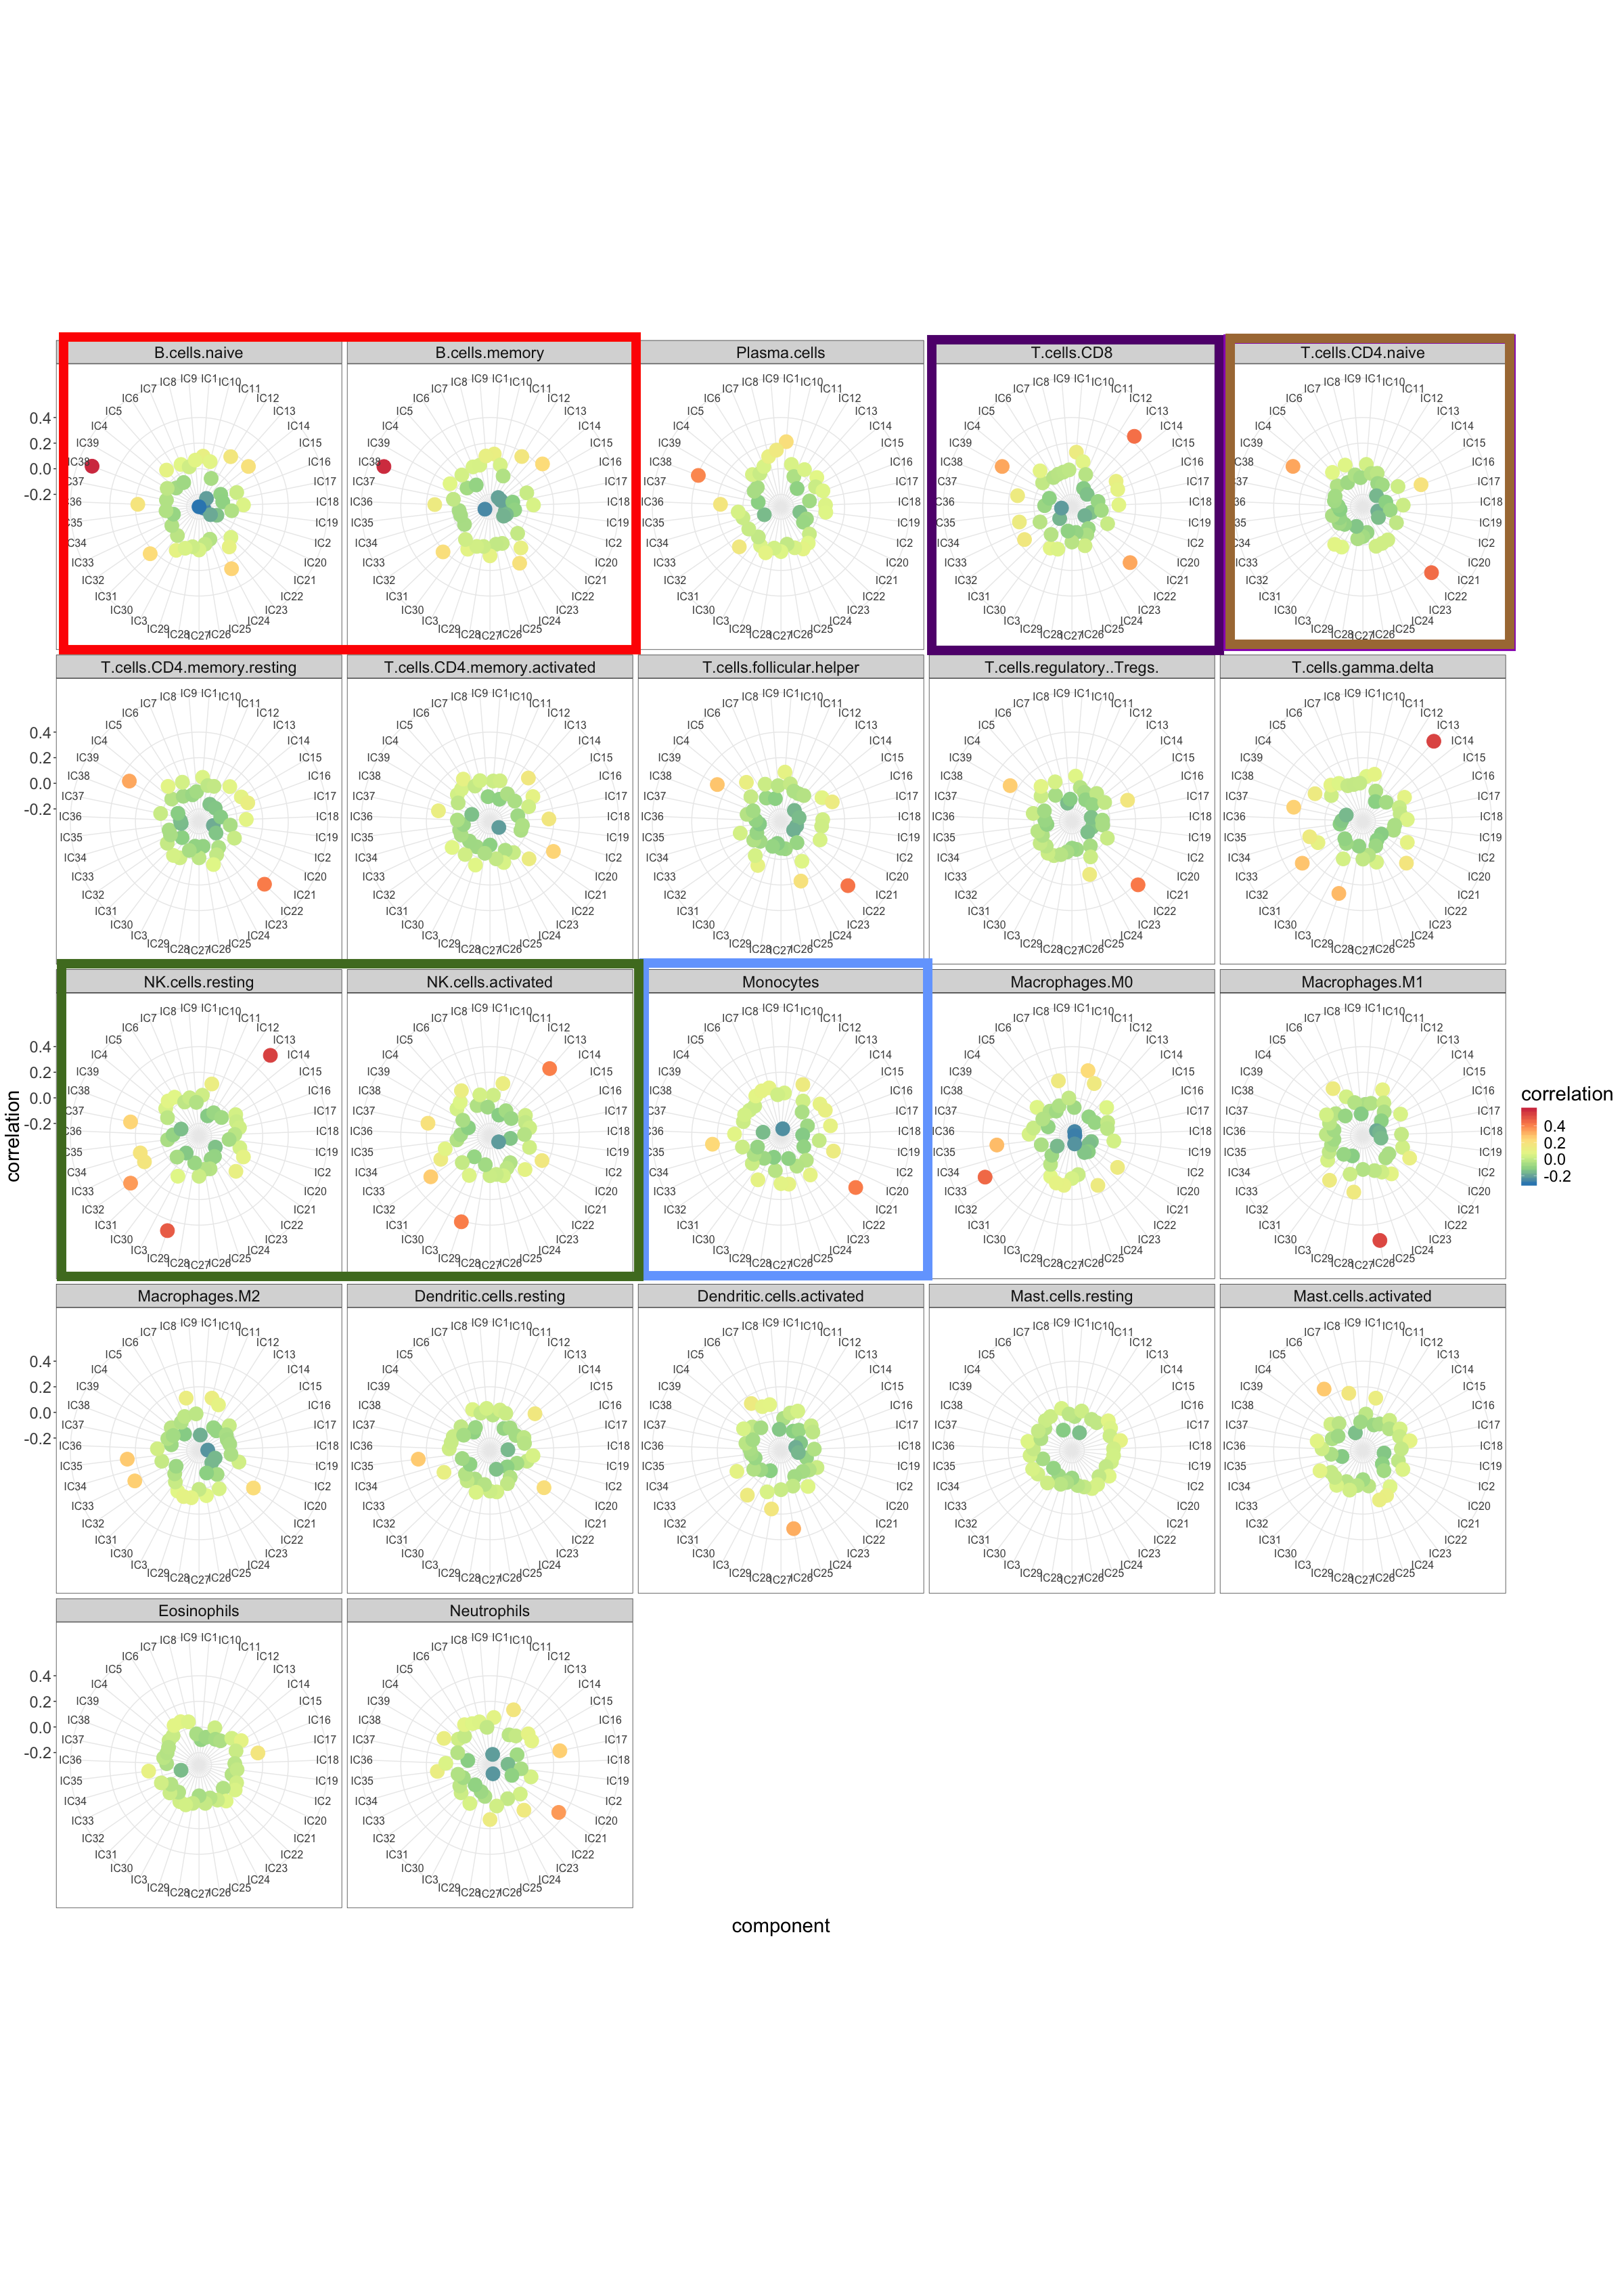
\includegraphics[width=1\linewidth]{figures-ext/radarBlood} 

}

\caption[Correlation between independent components and reference immune cell-type metagenes]{\textbf{Correlation between independent components
and reference immune cell-type metagenes}. All correlation and reference
cell types are illustrated. Surrounded by color squares are the most
important panels for decision making and matching cell types measures as
well with CyTOF, used for further comparison.}\label{fig:radarB}
\end{figure}







\begin{figure}

{\centering 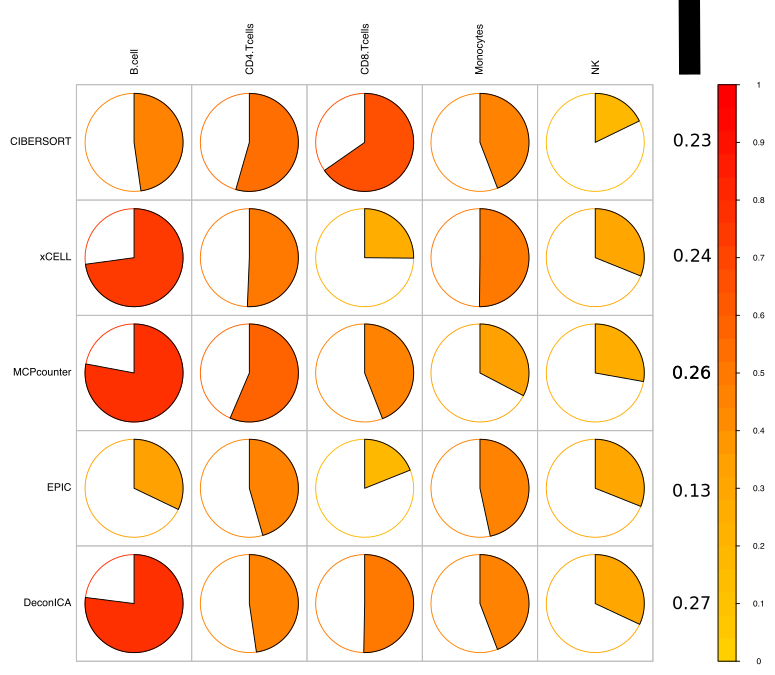
\includegraphics[width=0.7\linewidth]{figures-ext/comparisonR2} 

}

\caption[Estimation of abundance of immune cell types in PBMC transcriptome of 104 healthy donors]{\textbf{Estimation of abundance of immune cell
types in PBMC transcriptome of 104 healthy donors}. Five different
methods (xCell \citep{Aran2017}, CIBERSORT \citep{Newman2015}, EPIC
\citep{Racle2017}, MCPcounter \citep{Becht2016}, DeconICA
\citep{Czerwinska2018}), were applied to compare estimated proportions
and CyTOF measured proportions of five cell types: B-cells, CD8
T-.cells, CD4 T-cells, Monocytes and NK as they were identified with
DeconICA and measured proportions were available. In the case of a not
exact match of cell types between the CyTOF and deconvolutions method,
best correlation was reported. The average \(R^2\) is computed as an
average of \(R^2\) for each cell types by the method. DeconICA slightly
overperforms existing methods.}\label{fig:comparison}
\end{figure}














Besides, the markers discovered from data by DeconICA, are not
significantly overlapping with markers used by MCPcounter or xCell (Fig.
\ref{fig:venn}) (for EPIC and CIBERSORT list of specific cell-markers is
provided as they use a basis matrix).

\begin{figure}

{\centering 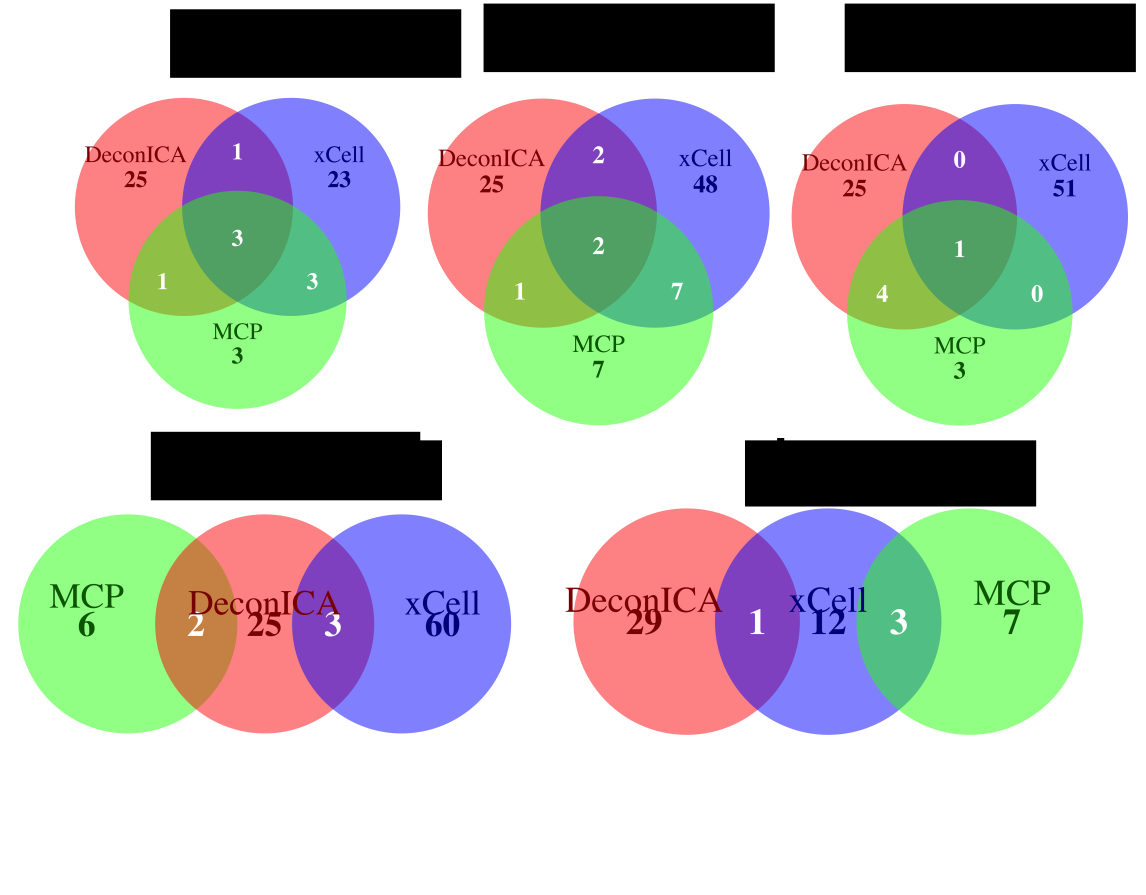
\includegraphics[width=1\linewidth]{figures-ext/venn} 

}

\caption[Comparison of markers used by different deconvolution methods]{\textbf{Comparison of markers used by different
deconvolution methods}: markers of xCell, MCPcounter, and markers
discovered from data by DeconICA are compared. Venn diagrams illustrate
insignificant overlap between the specific markers list for each cell
type.}\label{fig:venn}
\end{figure}







\hypertarget{summary-4}{%
\section{Summary}\label{summary-4}}

I developed a DeconICA method and R package that allow decomposition of
omic data into components. Based on stabilized fastICA decomposition I
demonstrated that DeconICA could estimate cell proportions of immune
cell types in PMBC transcriptome with better performance than previously
published tools without an \emph{a priori} use of cell-type signatures.
The \emph{marker} genes discovered with ICA, proven to evaluate cell
abundance correctly, turned out to be different from the markers used by
knowledge-based supervised deconvolution methods.

Even though the first release of DeconICA is published online
\citep{Czerwinska2018} and fully functional, some improvements can still
be considered in the future. Examples using other unsupervised
deconvolution methods can be included to demonstrate that the pipeline
is not limited to ICA. An interactive online interface can be built with
R shiny for instance. Also, more automatized label attribution and
confidence of the match between a reference metagene and a component
should be added. I would like also demonstrate the use of DeconICA with
methylome data.

Main limitations of DeconICA are

\begin{itemize}
\tightlist
\item
  the need to work with many samples (\textgreater{}100)
\item
  the interpretation that requires manual adjustments
\item
  the number of detected cell types usually lower than other tools
\item
  the abundance scores that cannot be directly interpreted as
  percentages of sample content
\item
  it is not guaranteed to find a source of the desired cell-type
\end{itemize}

Main advantages of DeconICA are:

\begin{itemize}
\tightlist
\item
  the possibility to discover new markers from data
\item
  context independence (no a priori use of blood-derived cell-type
  signatures)
\item
  universality: DeconICA can identify not only cell types but also other
  factors governing cancer transcriptomes, can also be applied for
  different purposes with a little adjustment
\item
  sequencing/ microarray platform independence
\item
  data normalization independence
\item
  speed (a formal benchmark is to be provided, but the analysis of the
  biggest available transcriptomic dataset METABRIC (1980 samples) can
  be analyzed within less than 1 hour)
\item
  user-friendly form of R package, tutorials, and transparent,
  open-source code
\end{itemize}

So far, the tool does not have many users from outside my research
group. I hope it will change once the tool is published in a scientific
journal.

An ability to discover possible new marker genes of cell states can be
extremely interesting in cancer context where true cell-type
context-dependent signatures are not known. If this hypothesis is
correct, DeconICA should not only correctly evaluate cell-type
abundances but also give insight to context-dependent cell type/cell
state signatures.

In the next chapter, I will apply DeconICA to \textgreater{}100
transcriptomic datasets of different cancer types to identify
tumor-specific signatures of immune cell types, compare them and
describe their features.

\hypertarget{results}{%
\chapter{Comparative analysis of cancer immune
infiltration}\label{results}}

\emph{Selected content of this chapter is a part of a publication in
preparation}

\hypertarget{background}{%
\section{Background}\label{background}}

\hypertarget{methods-1}{%
\section{Methods}\label{methods-1}}

\hypertarget{data-sources}{%
\subsection{Data sources}\label{data-sources}}

\textbf{Bulk datasets}

\textbf{Single cell datasets}

\hypertarget{the-deconica-pipeline-on-bulk}{%
\subsection{The DeconICA pipeline on
bulk}\label{the-deconica-pipeline-on-bulk}}

Labeling components

post Data cleaning

\hypertarget{the-deconica-pipeline-on-single-cell}{%
\subsection{The DeconICA pipeline on single
cell}\label{the-deconica-pipeline-on-single-cell}}

\hypertarget{results-1}{%
\section{Results}\label{results-1}}

\begin{figure}

{\centering 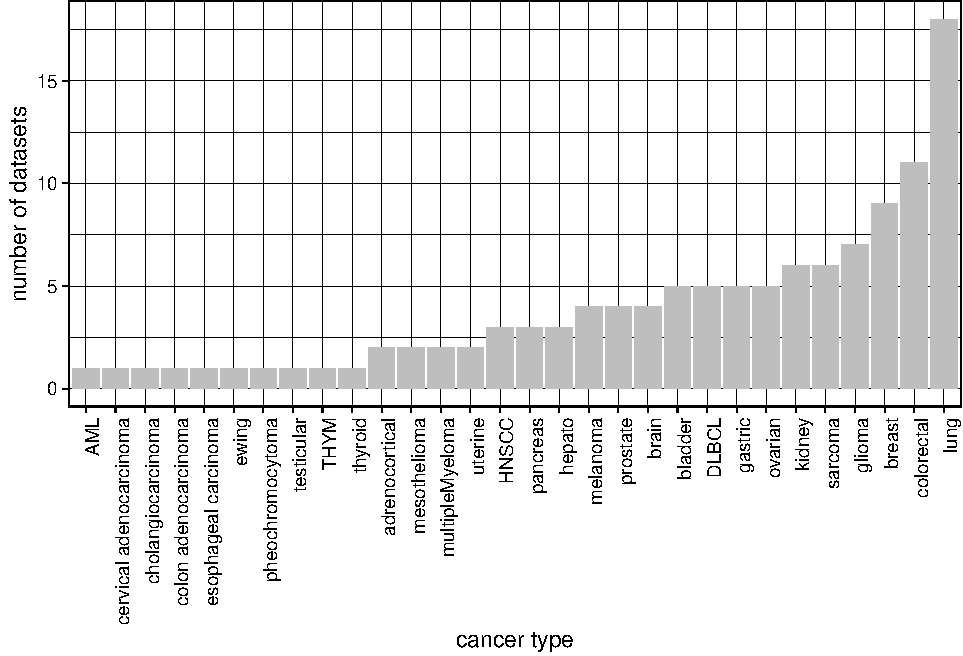
\includegraphics[width=0.8\linewidth]{UCzPhDThesis_files/figure-latex/datasetcount-1} 

}

\caption[Count of the dasets analyzed with DeconICA]{(ref:datasetcount-caption)}\label{fig:datasetcount}
\end{figure}

(ref:datasetcount-caption)

\begin{figure}

{\centering 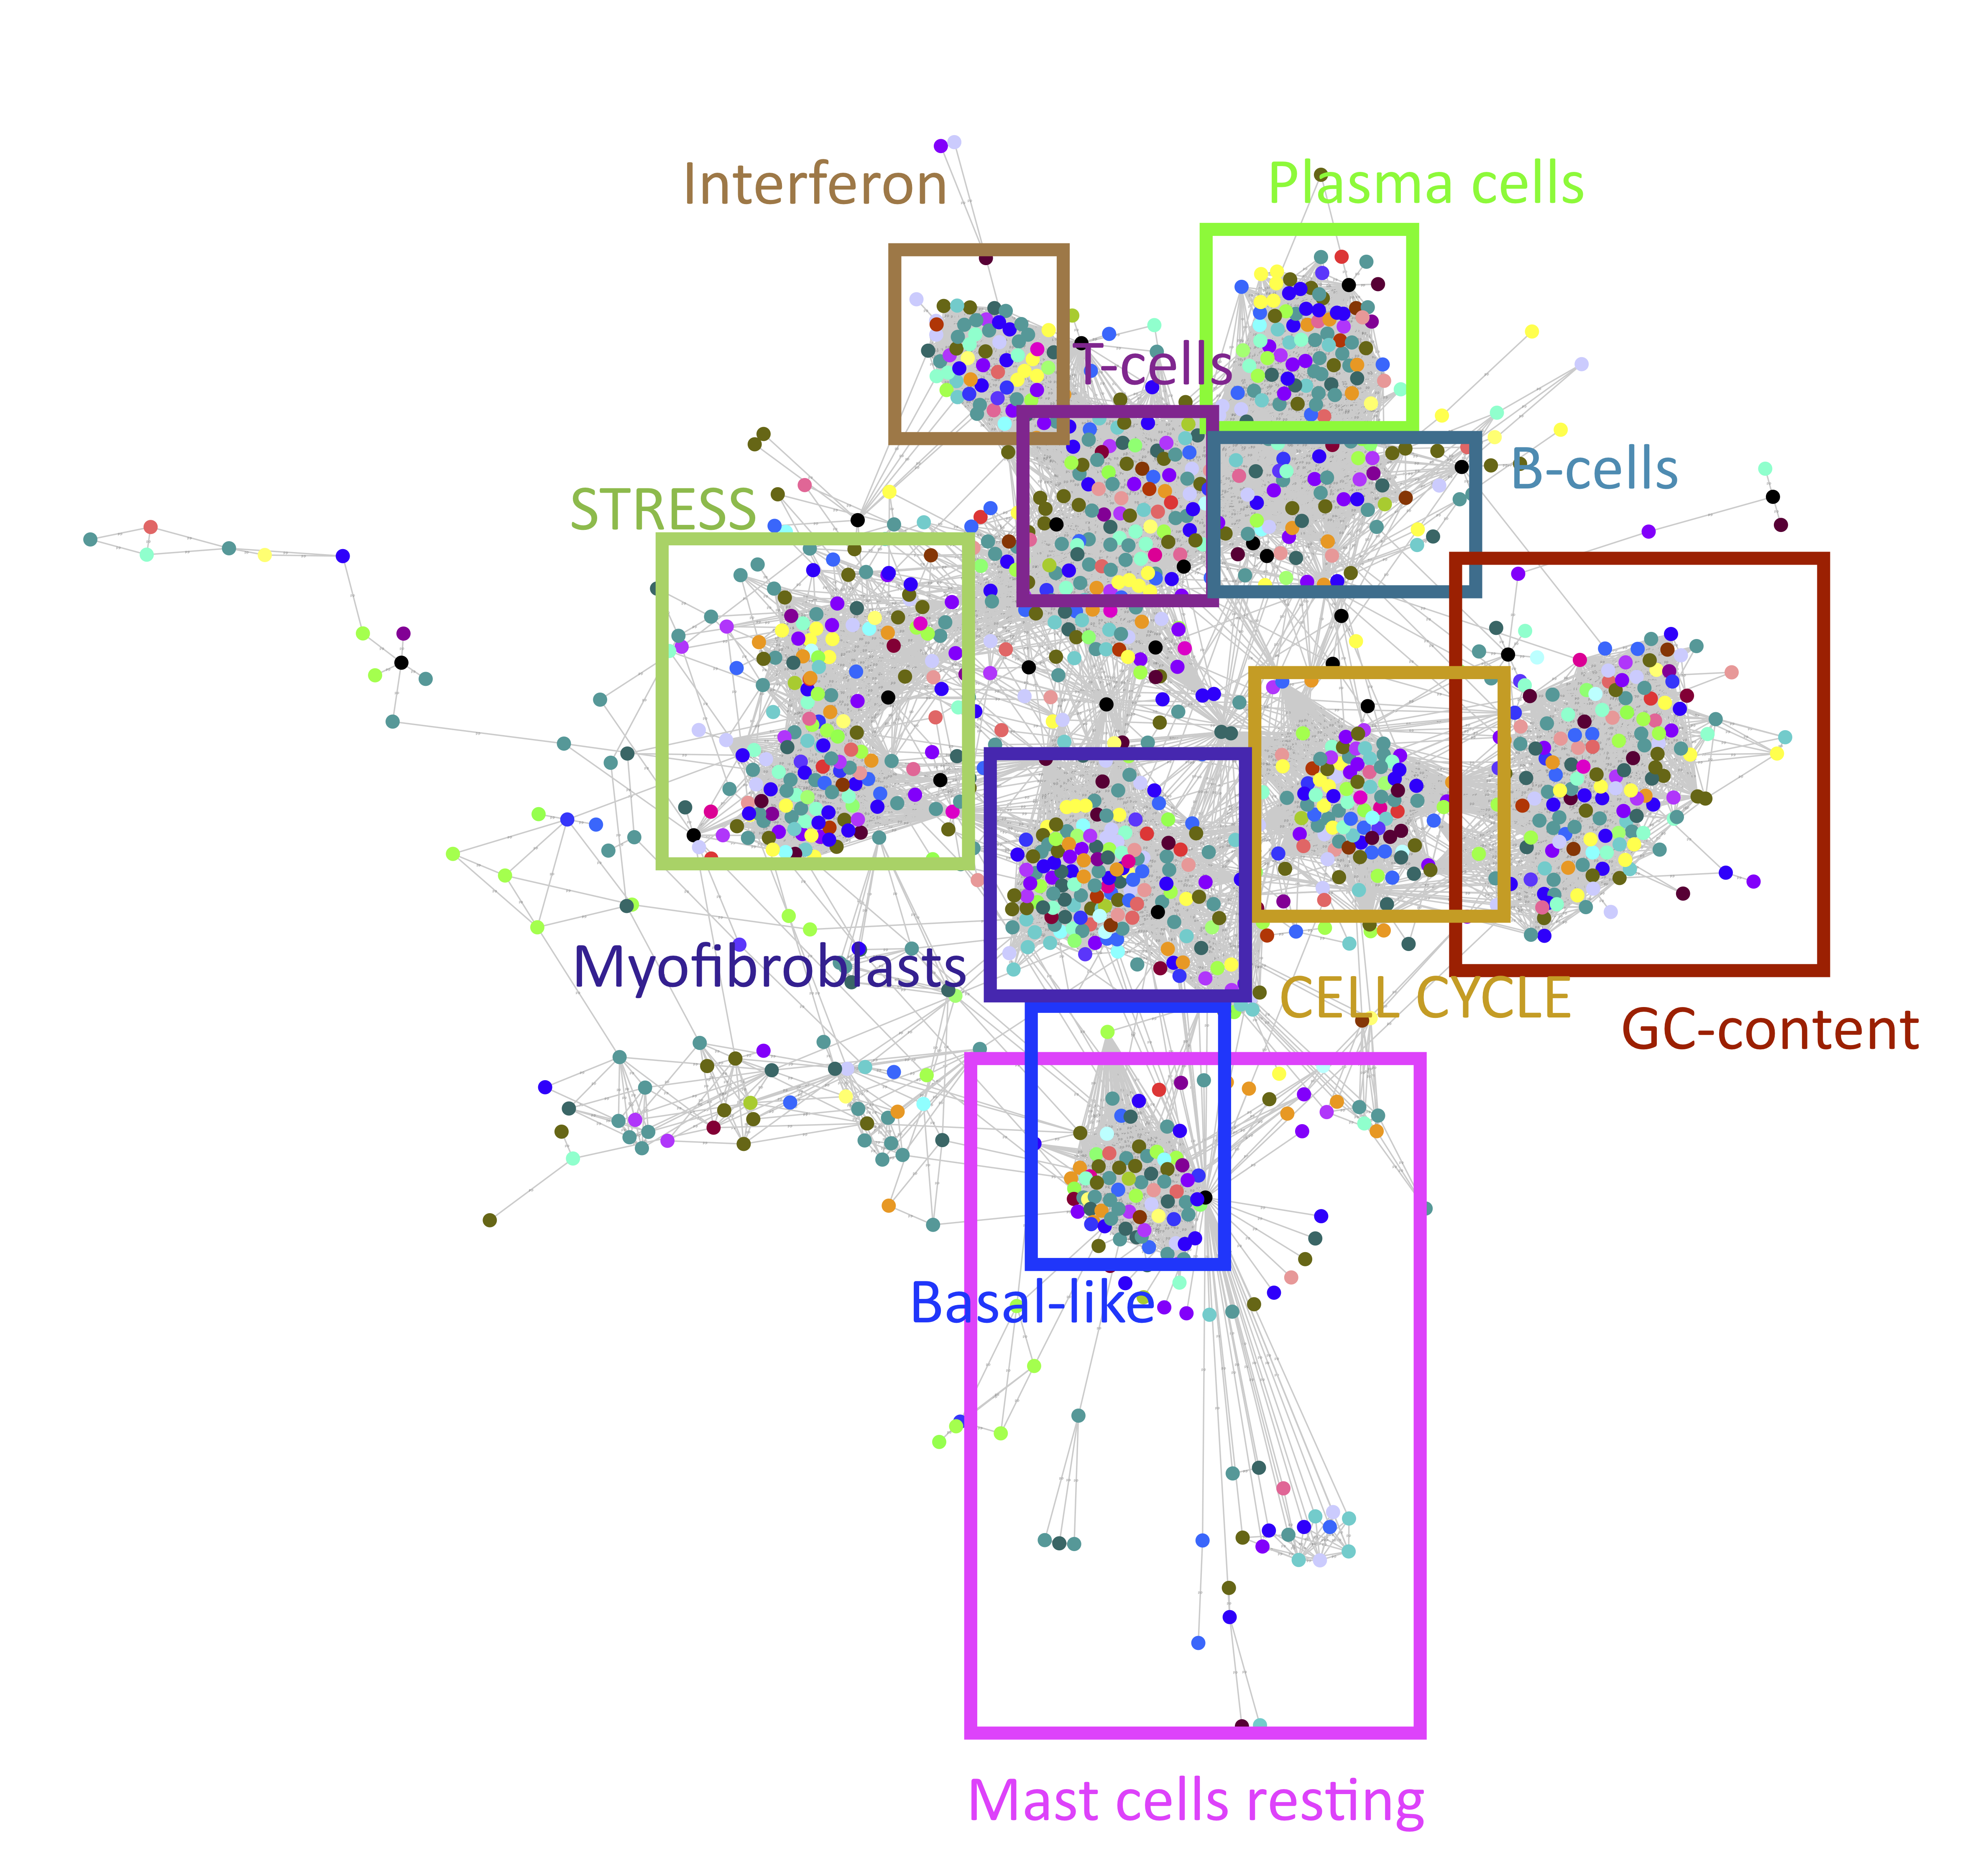
\includegraphics[width=1\linewidth,height=0.5\textheight]{figures-ext/full_02_recip_color_annot} 

}

\caption[Correlation graph of metagenes]{(ref:corrgraphfull-caption)}\label{fig:corrgraphfull}
\end{figure}

(ref:corrgraphfull-caption)

\begin{figure}

{\centering 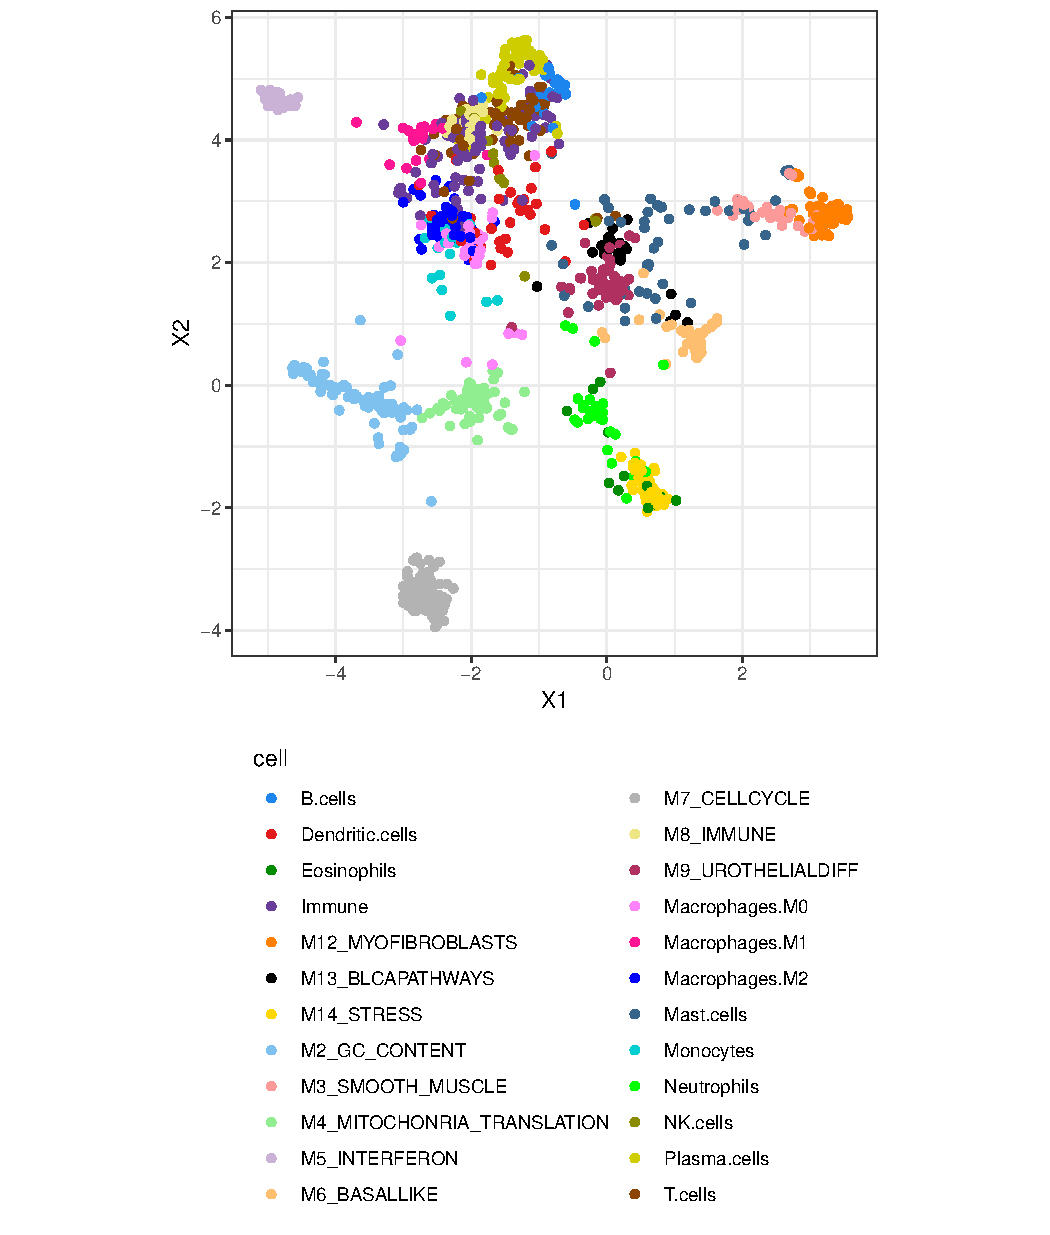
\includegraphics[width=0.9\linewidth]{figures-ext/umap_plot_cleaned} 

}

\caption[2D representation of labelled metagenes]{(ref:umapplotclean-caption)}\label{fig:umapplotclean}
\end{figure}

(ref:umapplotclean-caption)

\begin{figure}

{\centering 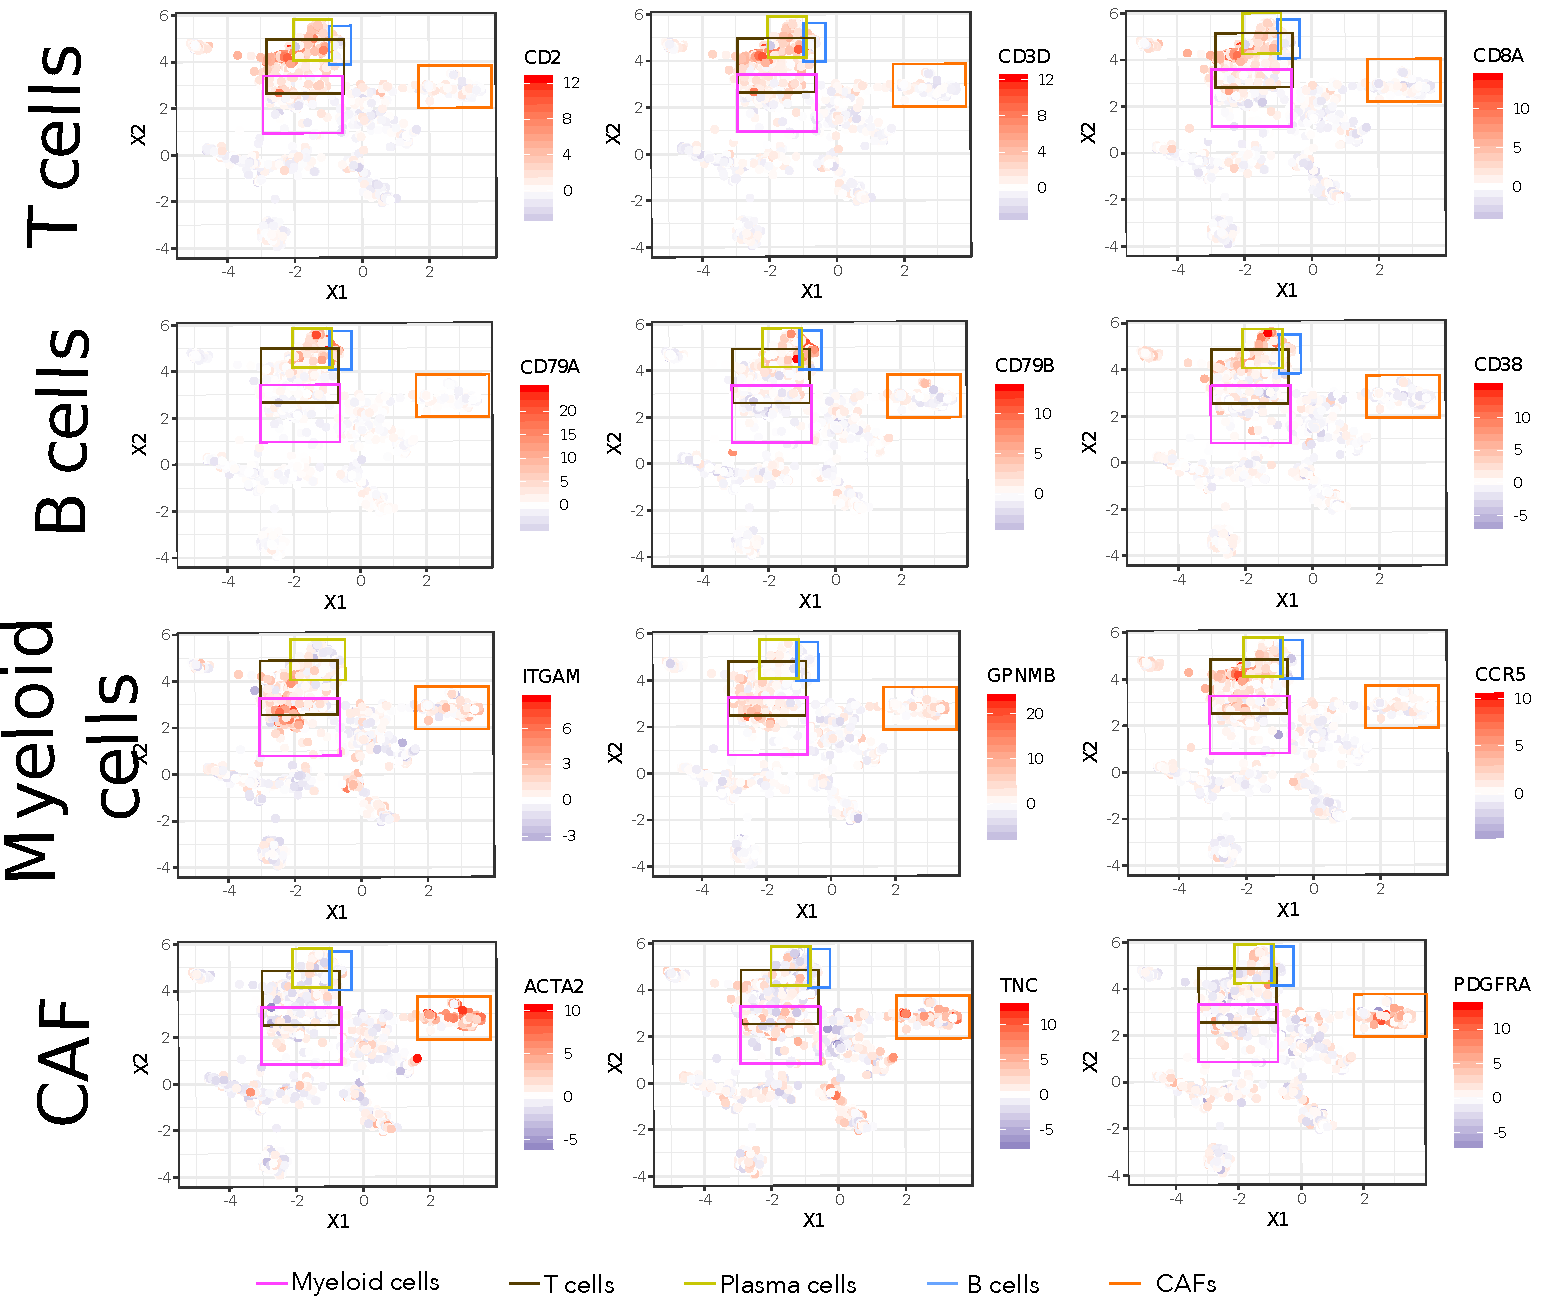
\includegraphics[width=1\linewidth]{figures-ext/panel_markers_labels_gates_legend} 

}

\caption[Cell markers expression in the metagenes]{(ref:panel-caption)}\label{fig:panel}
\end{figure}

(ref:panel-caption)

\begin{figure}

{\centering 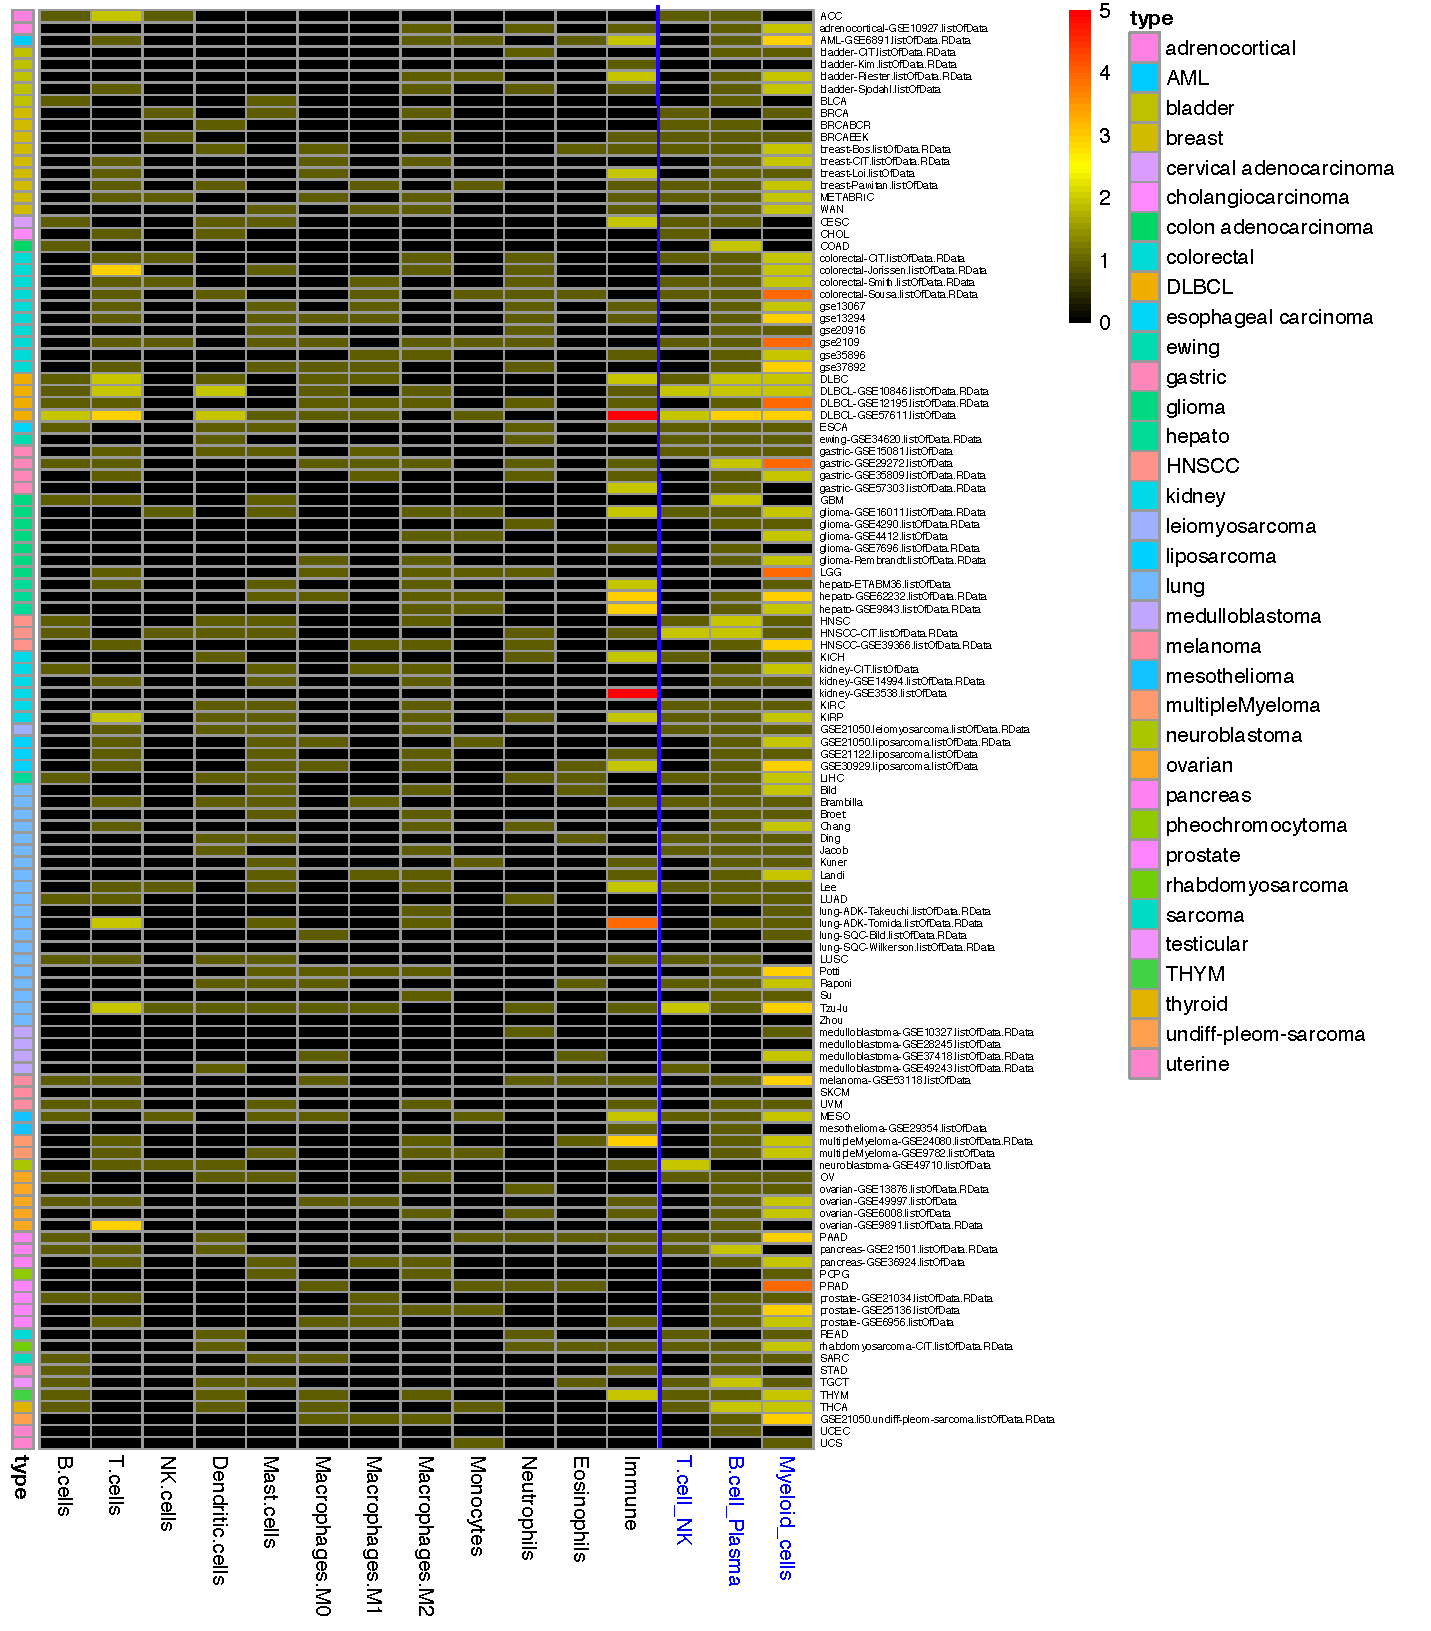
\includegraphics[width=1\linewidth]{figures-ext/count_detectability_immune_only} 

}

\caption[Cell markers expression in the metagenes]{(ref:countdectect-caption)}\label{fig:countdectect}
\end{figure}

(ref:countdectect-caption)

\begin{figure}

{\centering 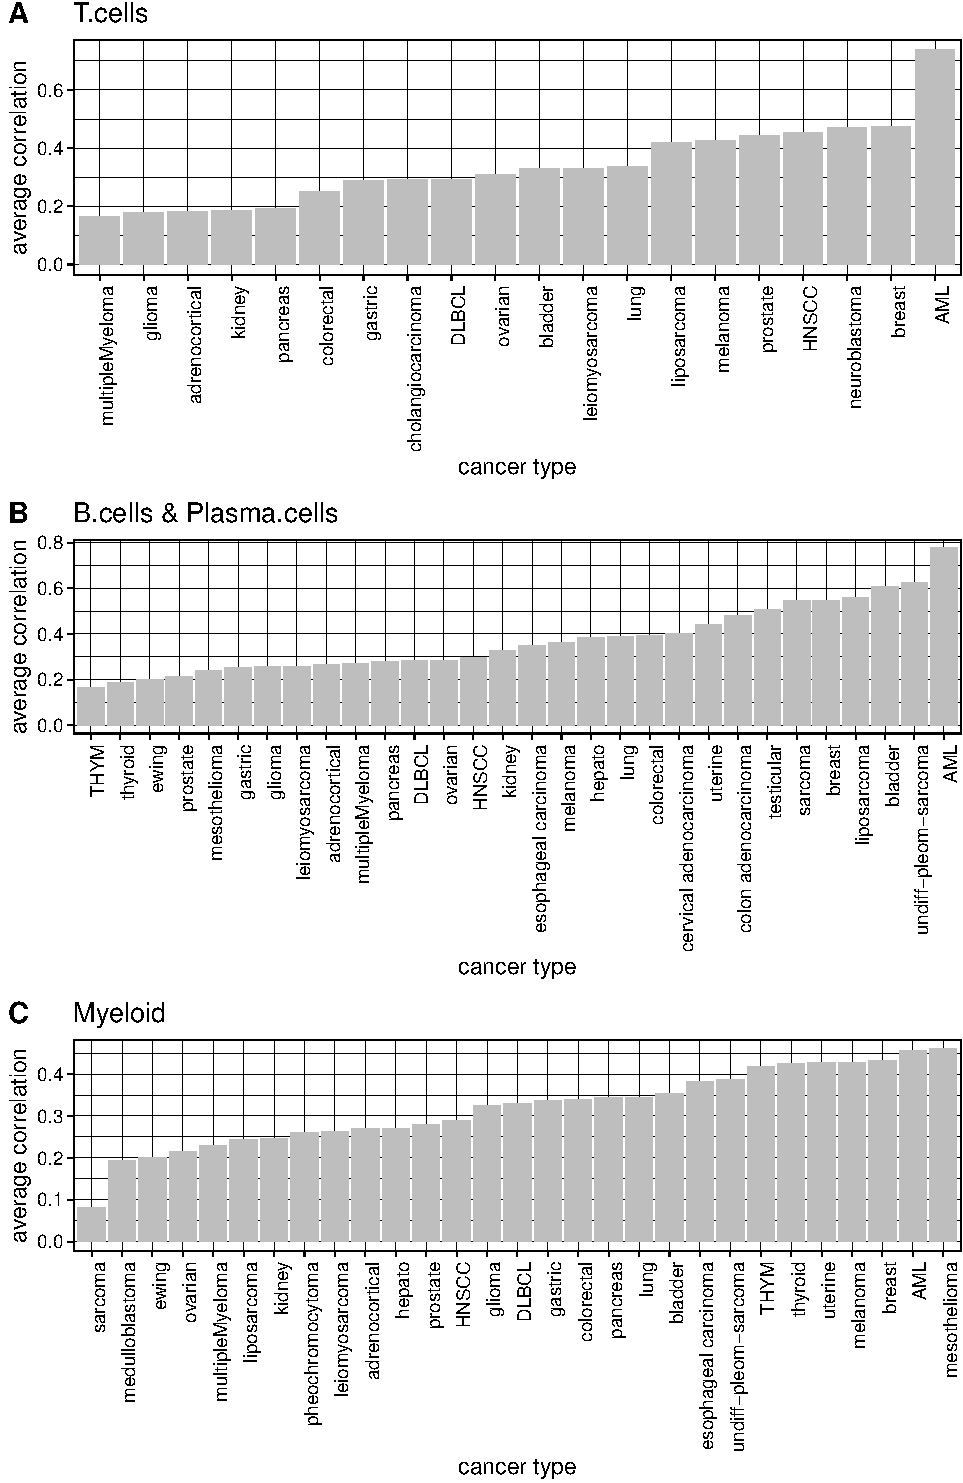
\includegraphics{UCzPhDThesis_files/figure-latex/corrbar-1} 

}

\caption[Correlation of cell-type metagenes with the refrence profiles]{(ref:corrbar-caption)}\label{fig:corrbar}
\end{figure}

(ref:corrbar-caption)

\begin{figure}

{\centering 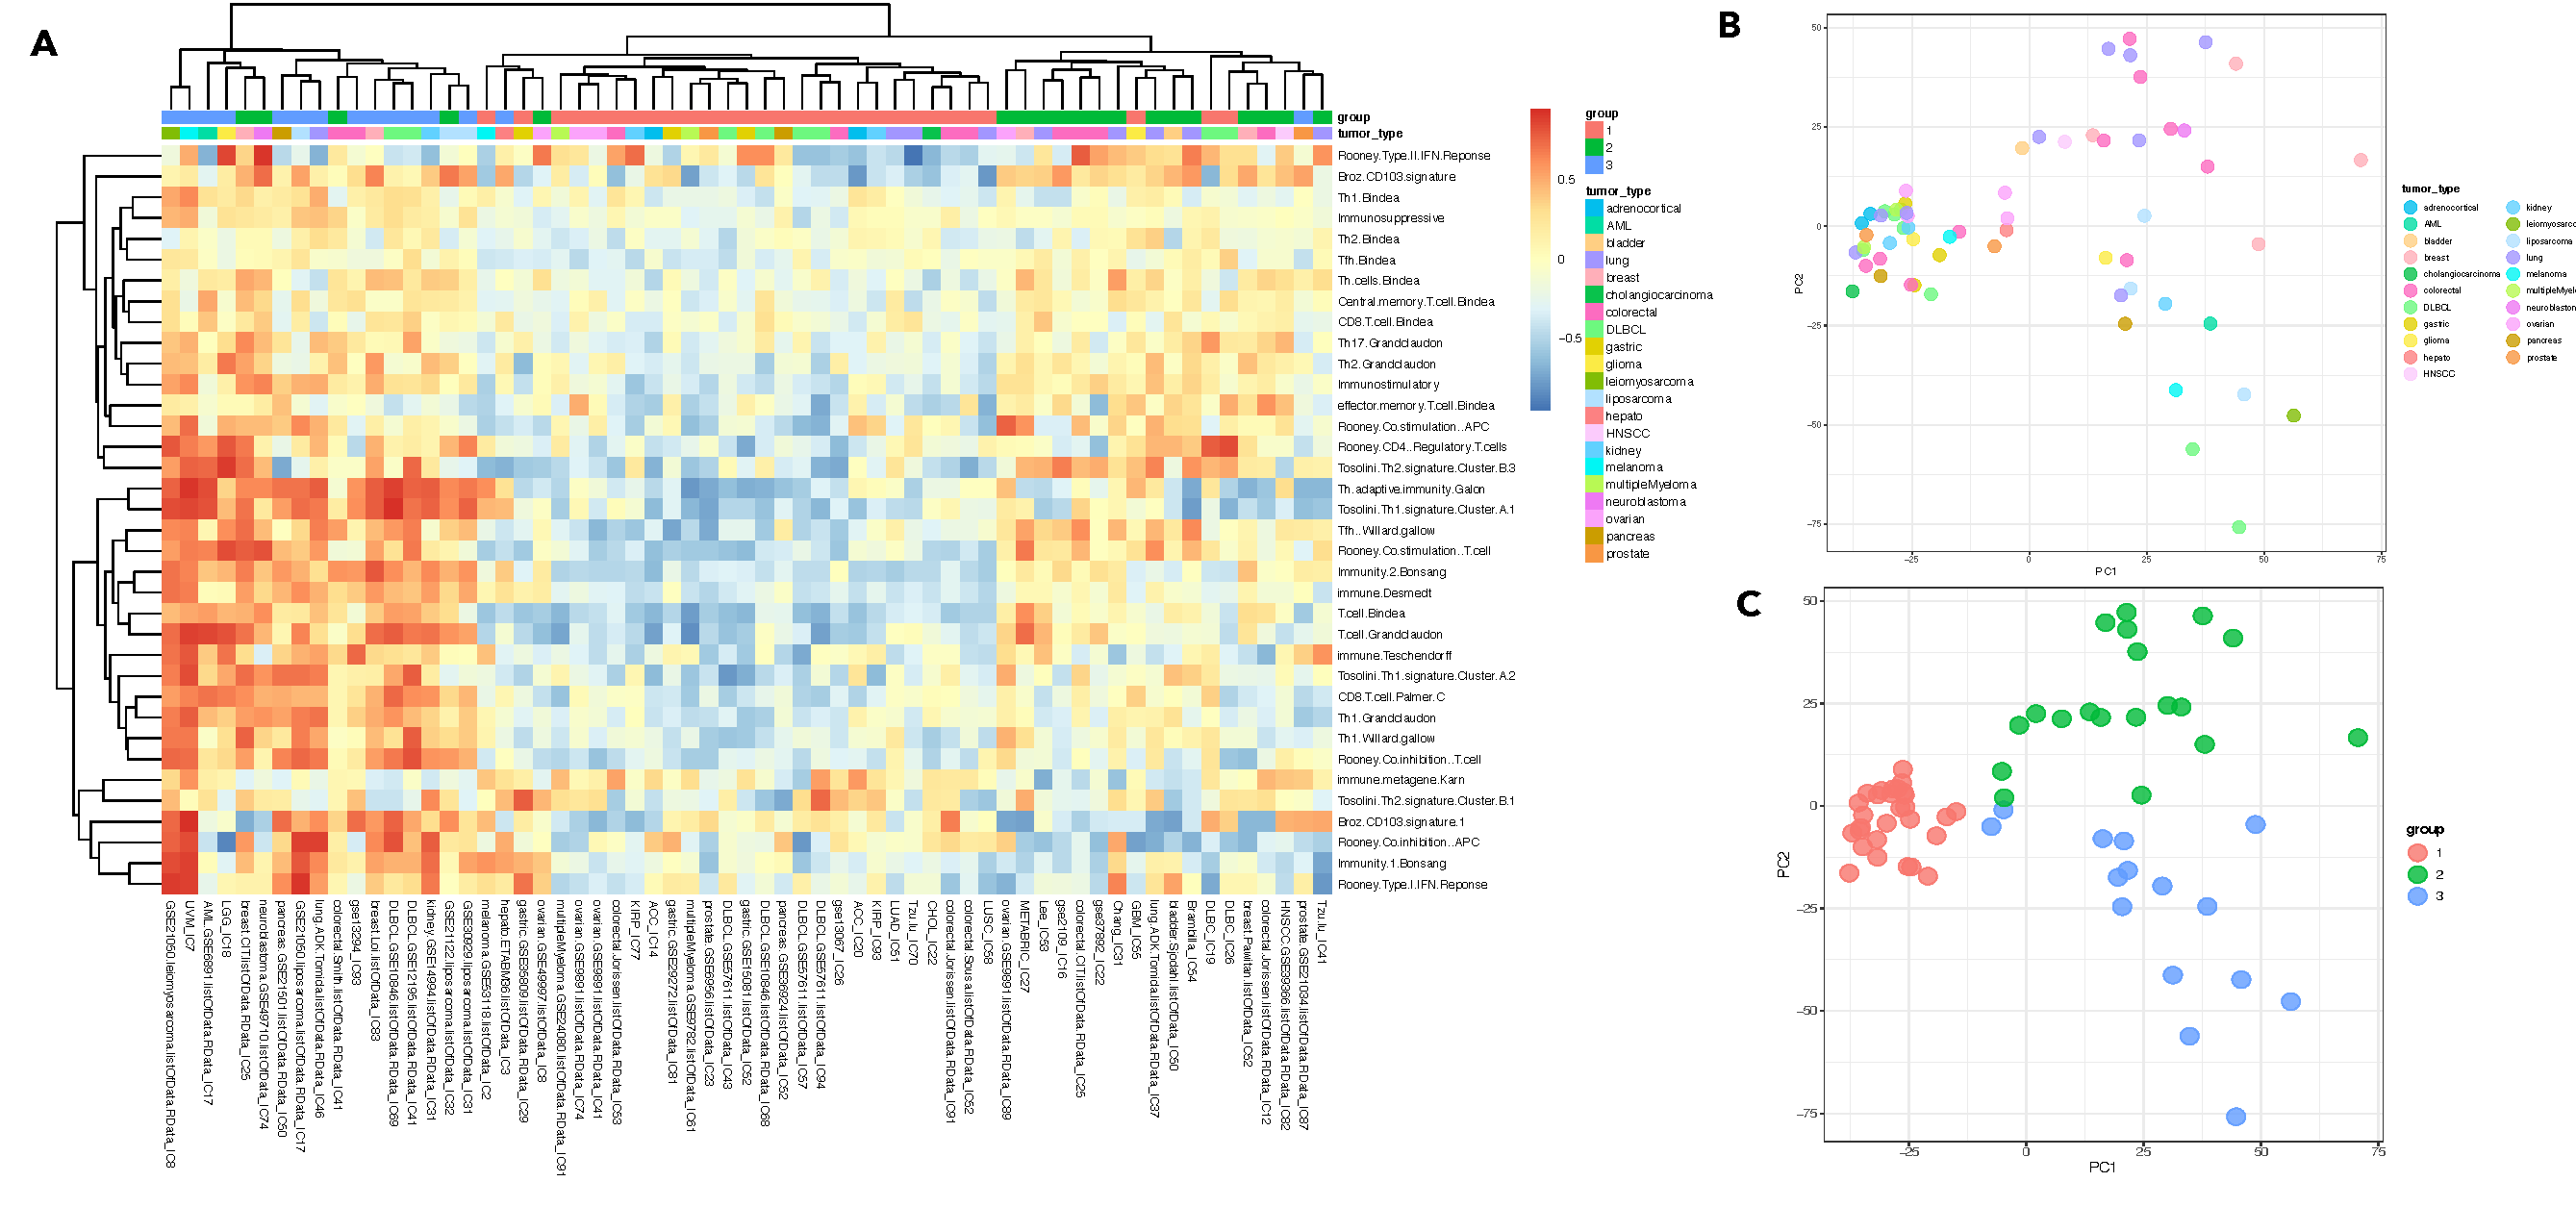
\includegraphics[width=7.5in,angle=90]{figures-ext/TcellDiv} 

}

\caption[Analysis of T cell diversity]{(ref:tcelldiv-caption)}\label{fig:tcelldiv}
\end{figure}

(ref:tcelldiv-caption)

\begin{figure}

{\centering 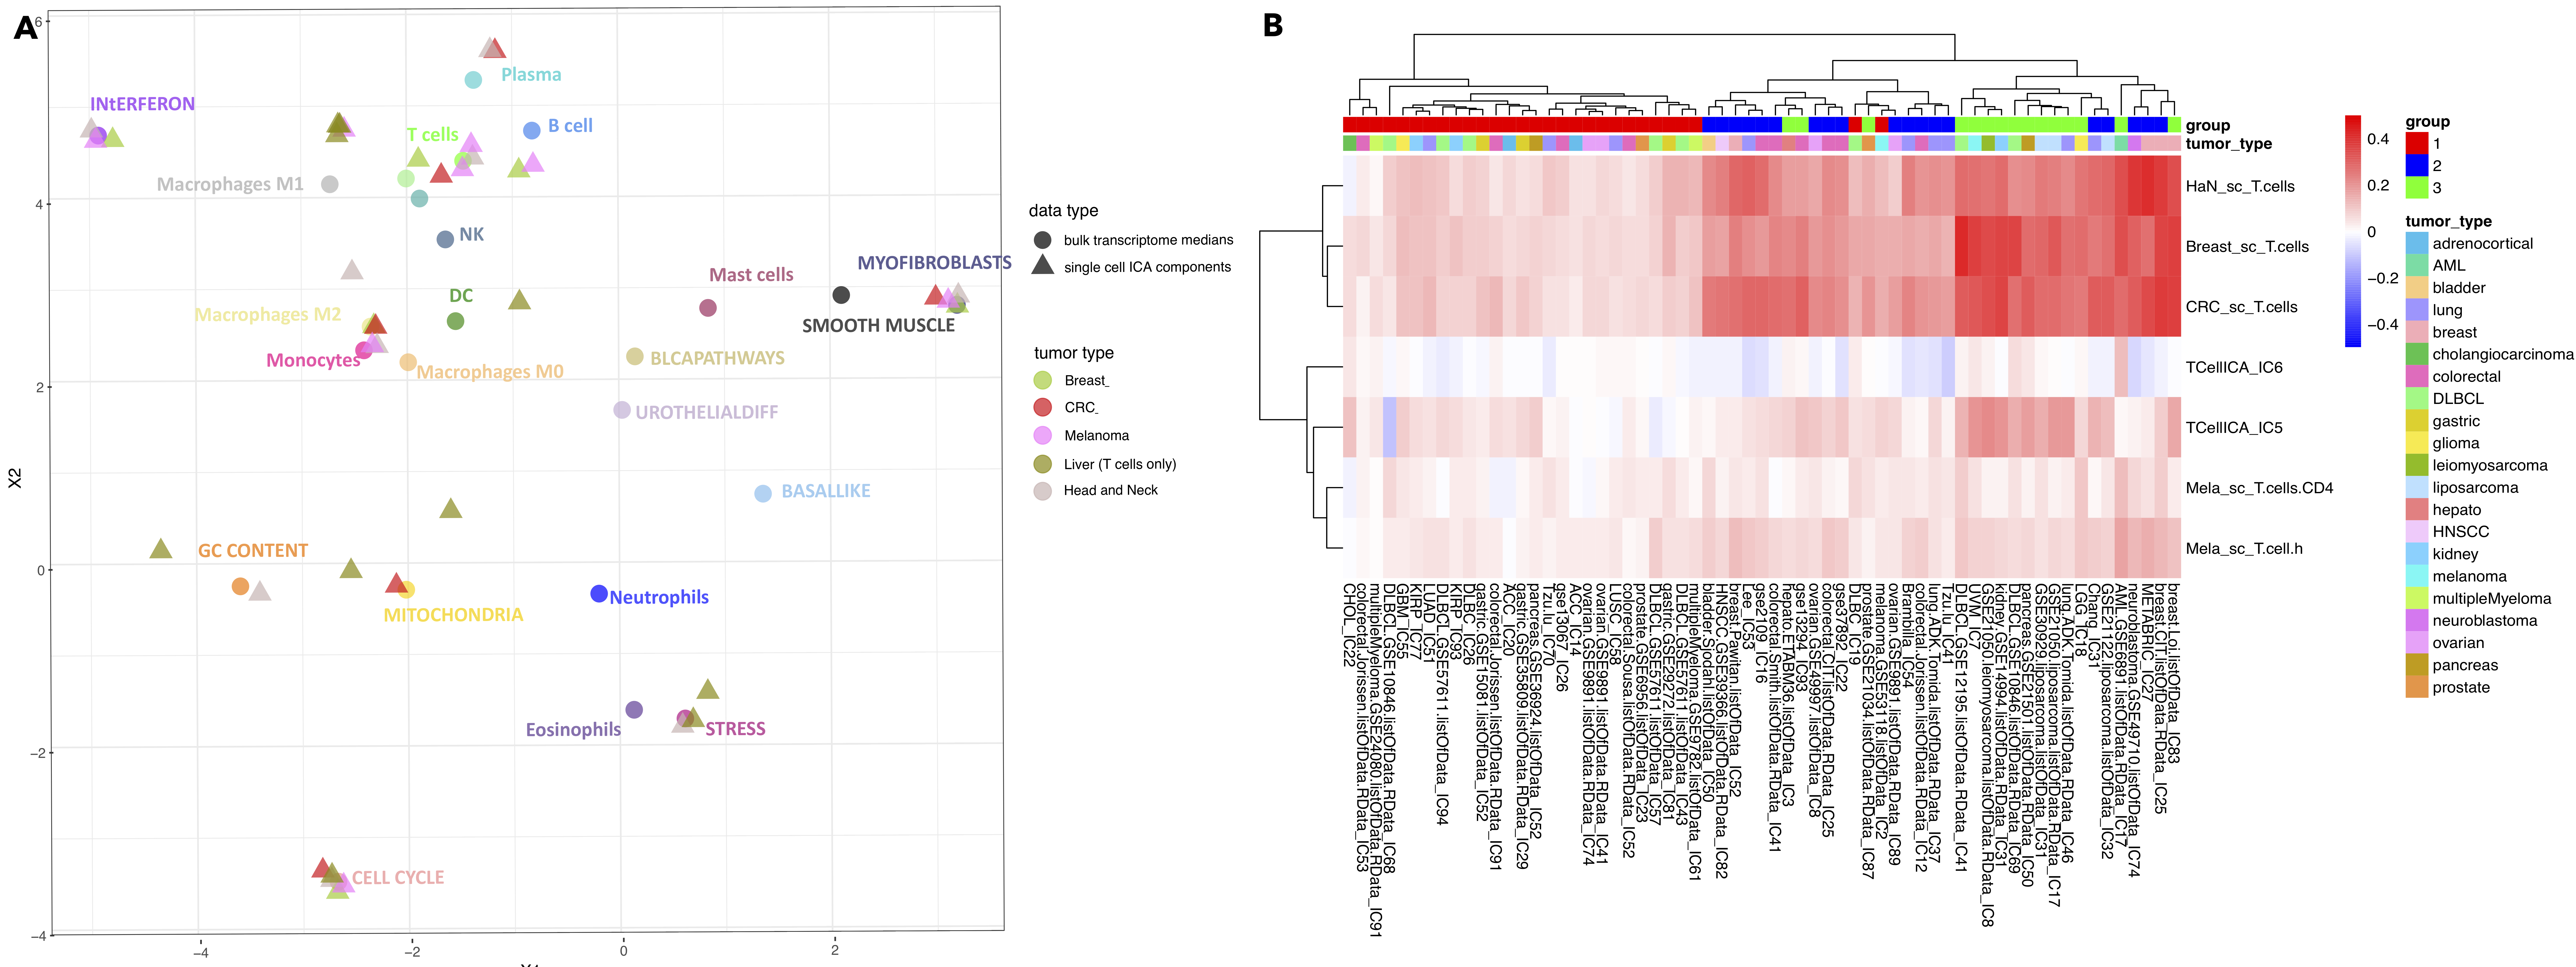
\includegraphics[width=7.5in,angle=90]{figures-ext/corr_sc_tcell_plot} 

}

\caption[Metagenes from single cell and bulk transcriptome]{(ref:scbulk-caption)}\label{fig:scbulk}
\end{figure}

\hypertarget{discussion}{%
\section{Discussion}\label{discussion}}

\hypertarget{conclussions}{%
\section{Conclussions}\label{conclussions}}

\newpage

\hypertarget{supplementary}{%
\section{Supplementary}\label{supplementary}}

\hypertarget{figures}{%
\subsection{Figures}\label{figures}}

\begin{figure}
\subfloat[1\label{fig:tsne1}]{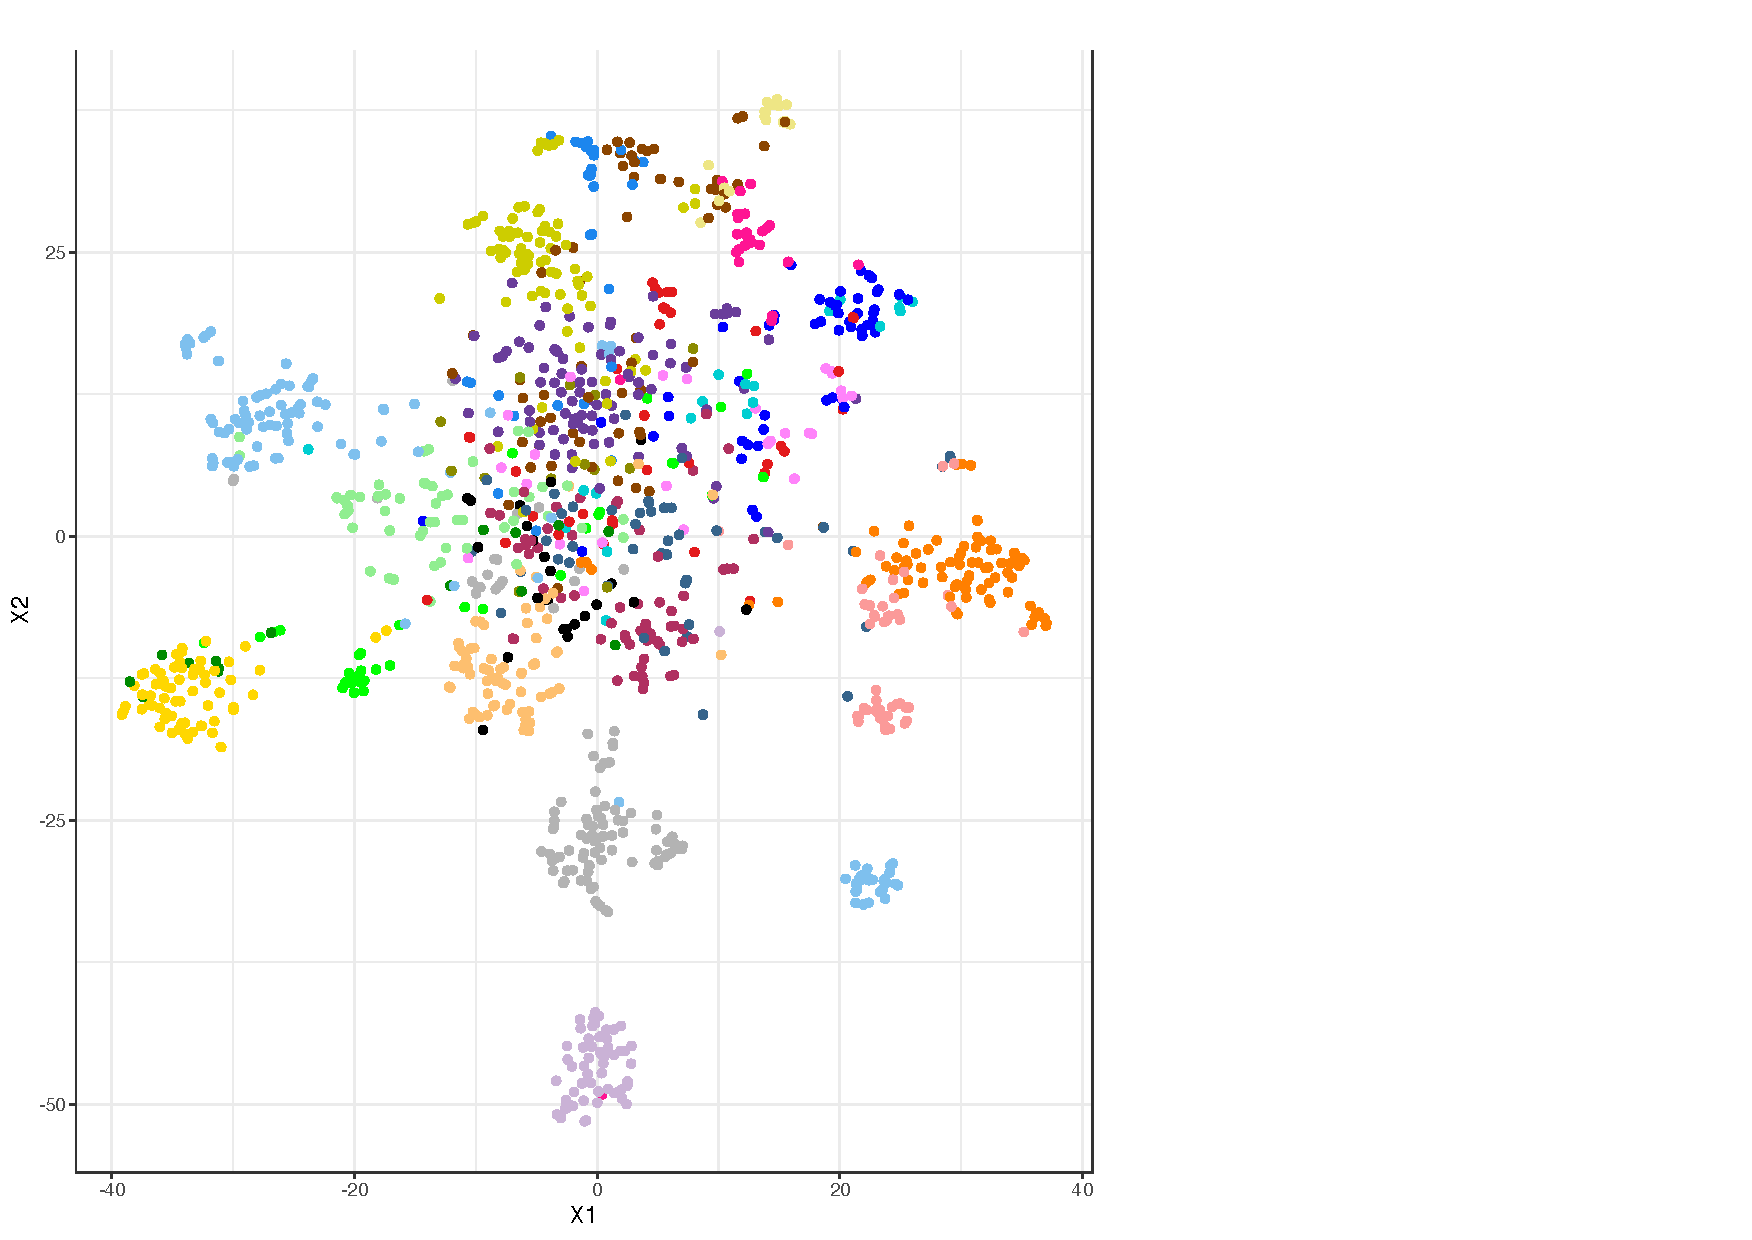
\includegraphics[width=0.33\linewidth]{./figures-ext/tsne_clean_P10_D100} }\subfloat[2\label{fig:tsne2}]{\includegraphics[width=0.33\linewidth]{./figures-ext/tsne_cleaned_P20_D50} }\subfloat[3\label{fig:tsne3}]{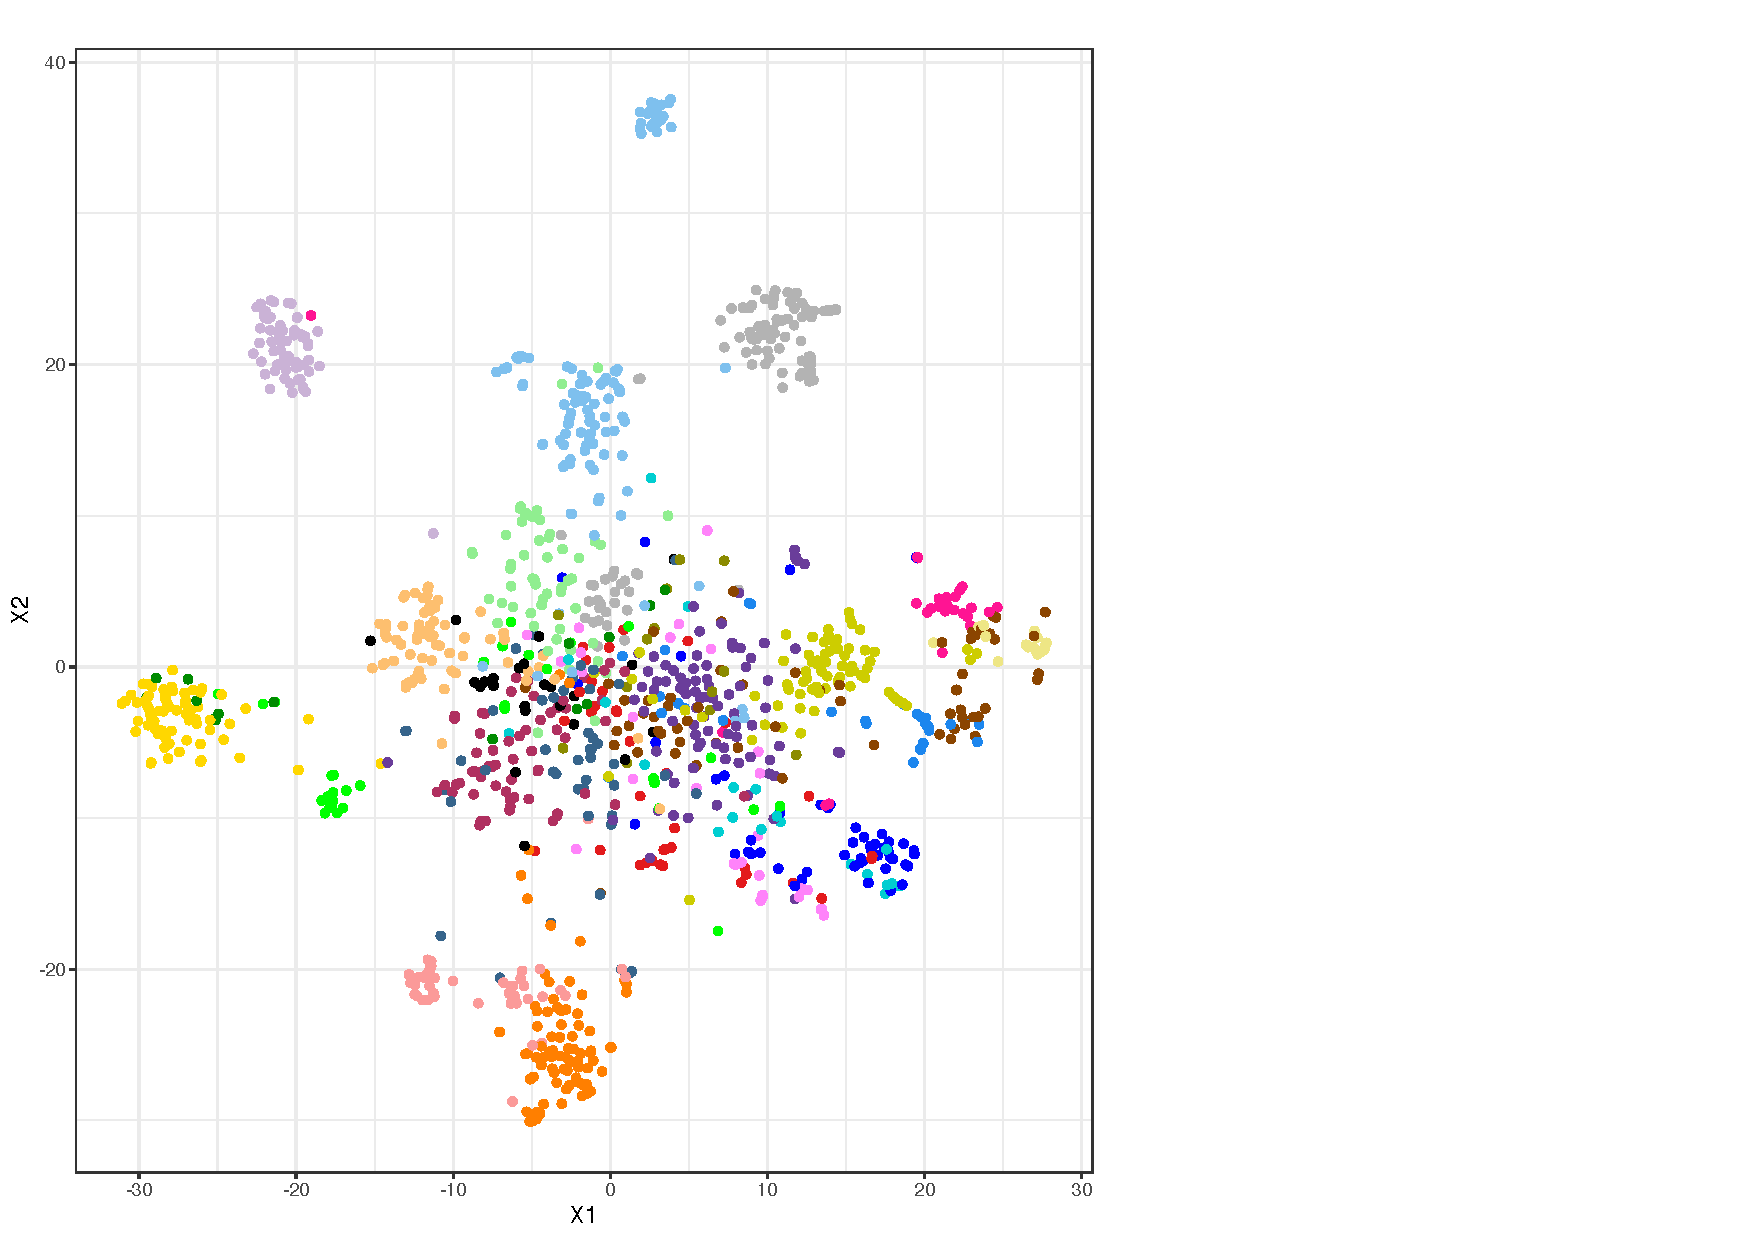
\includegraphics[width=0.33\linewidth]{./figures-ext/tsne-clean_P20_D100} }\caption[Metagenes 2D landscape, parameters testing]{(ref:tsne-caption)}\label{fig:tsne}
\end{figure}

(ref:tsne-caption)

\begin{figure}
\subfloat[1\label{fig:umap1}]{\includegraphics[width=2in]{./figures-ext/umap_nn5_dist0.2} }\subfloat[2\label{fig:umap2}]{\includegraphics[width=2in]{./figures-ext/umap_nn15_dist0.2} }\subfloat[3\label{fig:umap3}]{\includegraphics[width=2in]{./figures-ext/umap_nn20_dist0.2} }\caption[Metagenes 2D landscape, parameters testing]{(ref:umap-caption)}\label{fig:umap}
\end{figure}

(ref:umap-caption)

\begin{figure}

{\centering \includegraphics[width=1\linewidth]{figures-ext/ration_only_immune} 

}

\caption[Ratio of detected components by cancer type]{(ref:ratiodectect-caption)}\label{fig:ratiodectect}
\end{figure}

(ref:ratiodectect-caption)

\hypertarget{tables}{%
\subsection{Tables}\label{tables}}

\begingroup\fontsize{7}{9}\selectfont\rowcolors{2}{white}{gray!6}

\begin{longtable}[l]{>{\centering\arraybackslash}p{3em}>{\centering\arraybackslash}p{8em}>{\centering\arraybackslash}p{3em}>{\centering\arraybackslash}p{3em}>{\centering\arraybackslash}p{3em}>{\centering\arraybackslash}p{3em}>{\centering\arraybackslash}p{8em}>{\centering\arraybackslash}p{8em}>{\centering\arraybackslash}p{8em}c}
\caption[List of datasets]{\label{tab:bulklist}\textbf{Some capiton}.}\\
\hiderowcolors
\toprule
ID & Name & Cancer.type & Samples & Genes & Components & Source & Normalization & Technology & PMID\\
\midrule
\endfirsthead
\caption[]{\label{tab:bulklist}\textbf{Some capiton}. \textit{(continued)}}\\
\toprule
ID & Name & Cancer.type & Samples & Genes & Components & Source & Normalization & Technology & PMID\\
\midrule
\endhead
\
\endfoot
\bottomrule
\endlastfoot
\showrowcolors
1 & ACC & adrenocortical & 78 & 20501 & 54 & TCGA & custom & several & NA\\
2 & adrenocortical-GSE10927 & adrenocortical & 65 & 20621 & 36 & GSE10927 & quantile-normalized and log transformed as described & Affymetrix HG\_U133\_plus\_2 arrays & 19147773\\
3 & AML-GSE6891 & AML & 536 & 32194 & 100 & GSE6891 & MAS5.0 & Affymetrix HG-U133 plus 2 & 20522712\\
4 & Bild & lung & 111 & 33193 & 90 & GSE3141 & custom (see Bild et al.) & Affymetrix Human U133 2.0 plus arrays & 16273092\\
5 & bladder-CIT & bladder & 85 & 32194 & 56 & E-MTAB-1940 & custom & Affymetrix GeneChip Human Genome U133 Plus 2.0 & 24142880\\
\addlinespace
6 & bladder-Kim & bladder & 61 & 24533 & 28 & GSE13507 & quantile normalization, log2-transformed and median-centered across samples & Illumina human-6 v2.0 expression beadchip & 20059769\\
7 & bladder-Riester & bladder & 78 & 32194 & 49 & GSE31684 & GCRMA & Affymetrix Human Genome U133 Plus 2.0 Array & 22228636\\
8 & bladder-Sjodahl & bladder & 93 & 18581 & 62 & GSE32894 & median scaling & Illumina HumanHT-12 V3.0 expression beadchip & 22553347\\
9 & BLCA & bladder & 408 & 20501 & 100 & TCGA & custom & Illumina HiSeq & 24476821\\
10 & Brambilla & lung & 334 & 32396 & 100 & ? & ? & hgu133plus2 & ?\\
\addlinespace
11 & BRCA & breast & 1085 & 20501 & 100 & TCGA & custom & several & 23000897\\
12 & BRCABCR & breast & 1127 & 6837 & 100 & Fusion of 6 datasets from GEO: GSE6532, GSE3494, GSE1456, GSE7390, GSE5327, and ArrayExpress E-TABM-158 & see methods of Reyal et al., 2011 & Affymetrix HG-U133a & 21655258\\
13 & BRCABEK & breast & 197 & 21755 & 100 & GSE23720 & GCRMA & Affymetrix HG-U133Plus2.0 & 21339811\\
14 & breast-Bos & breast & 204 & 32194 & 100 & GSE12276 & GeneSpring 7.2 & Affymetrix HG-U133A & 19421193\\
15 & breast-CIT & breast & 537 & 32194 & 100 & ArrayExpress E-MTAB-365 & GCRMA & Affymetrix HG-U133Plus2.0 & 21785460\\
\addlinespace
16 & breast-Loi & breast & 327 & 19789 & 100 & gse6532 & custom & Affymetrix Human Genome U133A & NA\\
17 & breast-Pawitan & breast & 159 & 19789 & 100 & GSE1456 & global mean method & Affymetrix Human Genome U133A and U133B Array & 16280042\\
18 & Broet & lung & 72 & 33193 & 46 & GSE10445 & custom & Affymetrix Human Genome U133 Plus 2.0 Array & 20810387\\
19 & CESC & cervical adenocarcinoma & 303 & 20501 & 100 & TCGA & custom & Illumina HiSeq 2000 & 28112728\\
20 & Chang & lung & 90 & 14376 & 52 & GSE14814 & RMA & Affymetrix Human Genome U133A Array & 20823422\\
\addlinespace
21 & CHOL & liver & 36 & 20501 & 25 & TCGA & custom & Illumina HiSeq 2000 Genome Analyzers & 28297679\\
22 & COAD & colorectal & 278 & 20501 & 100 & TCGA & custom & several & 22810696\\
23 & colorectal-CIT & colorectal & 566 & 32194 & 100 & GSE39582 & ComBat & Affymetrix Human Genome U133 Plus 2.0 Array & 23700391\\
24 & colorectal-Jorissen & colorectal & 290 & 32194 & 100 & GSE14333 & custom & Affymetrix Human Genome U133 Plus 2.0 Array & 19996206\\
25 & colorectal-Smith & colorectal & 101 & 32194 & 61 & GSE17538 & NA & NA & NA\\
\addlinespace
26 & colorectal-Sousa & colorectal & 90 & 32194 & 58 & GSE33113 & fRMA & Affymetrix Human Genome U133 Plus 2.0 Array & 22496204\\
27 & Ding & lung & 75 & 33193 & 51 & GSE12667 & custom & Affymetrix Human Genome U133 Plus 2.0 Array & 18948947\\
28 & DLBC & DLBCL & 48 & 20501 & 34 & TCGA & custom & Illumina HiSeq 2000 Genome Analyzers & NA\\
29 & DLBCL-GSE10846 & DLBCL & 414 & 32194 & 100 & GSE10846 & NA & Affymetrix Human Genome U133 Plus 2.0 Array & 21546504\\
30 & DLBCL-GSE12195 & DLBCL & 83 & 32194 & 50 & GSE12195 & GenePattern & Affymetrix Human Genome U133 Plus 2.0 Array & 28314854\\
\addlinespace
31 & DLBCL-GSE57611 & DLBCL & 148 & 13239 & 100 & GSE57611 & custom & Affymetrix Human Genome U133A Array & 25042405\\
32 & ESCA & esophageal carcinoma & 182 & 20501 & 100 & TCGA & custom & Illumina HiSeq 2000 Genome Analyzers & 28052061\\
33 & ewing-GSE34620 & ewing & 117 & 32194 & 75 & GSE34620 & gcrma & Affymetrix Human Genome U133 Plus 2.0 Array & 22327514\\
34 & gastric-GSE15081 & gastric & 141 & 13105 & 100 & GSE15081 & custom & Hitachisoft AceGene Human Oligo Chip 30K 1 Chip Version & 20012501\\
35 & gastric-GSE29272 & gastric & 134 & 13239 & 100 & GSE29272 & custom & Affymetrix Human Genome U133A Array & 24867265\\
\addlinespace
36 & gastric-GSE35809 & gastric & 70 & 32194 & 43 & GSE35809 & custom & Affymetrix Human Genome U133 Plus 2.0 Array & 23684942\\
37 & gastric-GSE57303 & gastric & 70 & 32194 & 50 & GSE57303 & custom & Affymetrix Human Genome U133 Plus 2.0 Array & 24935174\\
38 & GBM & glioma & 760 & 20501 & 100 & TCGA & custom & several & 24120142\\
39 & glioma-GSE16011 & glioma & 284 & 32194 & 100 & GSE16011 & custom & Affymetrix GeneChip Human Genome U133 Plus 2.0 Array & 19920198\\
40 & glioma-GSE4290 & glioma & 180 & 32194 & 100 & GSE4290 & custom & Affymetrix Human Genome U133 Plus 2.0 Array & 16616334\\
\addlinespace
41 & glioma-GSE4412 & glioma & 85 & 19789 & 44 & GSE4412 & dCHIP & Affymetrix Human Genome U133A and U133B Array & 15374961\\
42 & glioma-GSE7696 & glioma & 80 & 32194 & 50 & GSE7696 & genewise-mean-centered, the log-scale robust multi-array average normalized & Affymetrix Human Genome U133 Plus 2.0 Array & 21642372\\
43 & glioma-Rembrandt & glioma & 534 & 32194 & 100 & https://caintergator.nci.nih.gov/rembrandt & MAS5 & Affymetrix HG U133 v2.0 Plus & 19208739\\
44 & GSE13067 & colorectal & 74 & 20307 & 47 & GSE13067 & MAS5.0 & Affymetrix Human Genome U133 Plus 2.0 Array & 19088021\\
45 & GSE13294 & colorectal & 155 & 20307 & 100 & GSE13294 & MAS5.0 & Affymetrix Human Genome U133 Plus 2.0 Array & 19088021\\
\addlinespace
46 & GSE20916 & colorectal & 100 & 20307 & 47 & GSE20916 & GCRMA & Affymetrix Human Genome U133 Plus 2.0 Array & 20957034\\
47 & GSE21050 & leiomyosarcoma & 85 & 32194 & 56 & GSE21050 & GCRMA & Affymetrix Human Genome U133 Plus 2.0 Array & 20581836\\
48 & GSE21050 & liposarcoma & 62 & 32194 & 43 & GSE21050 & GCRMA & Affymetrix Human Genome U133 Plus 2.0 Array & 20581836\\
49 & GSE21050 & undiff-pleom-sarcoma & 136 & 32194 & 100 & GSE21050 & GCRMA & Affymetrix Human Genome U133 Plus 2.0 Array & 20581836\\
50 & GSE2109 & colorectal & 277 & 20307 & 100 & GSE2109 & custom & Affymetrix Human Genome U133 Plus 2.0 Array & NA\\
\addlinespace
51 & GSE21122 & liposarcoma & 89 & 13239 & 53 & GSE21122 & RMA & Affymetrix Human Genome U133A Array & 20601955\\
52 & GSE30929 & liposarcoma & 140 & 13239 & 100 & GSE30929 & RMA & Affymetrix Human Genome U133A Array & 21335544\\
53 & GSE33382 & osteosarcoma & 84 & 24934 & 51 & GSE33382 & custom & Illumina human-6 v2.0 expression beadchip & 23688189\\
54 & GSE35896 & colorectal & 62 & 19040 & 40 & GSE35896 & RMA & Affymetrix Human Genome U133 Plus 2.0 Array & 23272949\\
55 & GSE37892 & colorectal & 130 & 20307 & 100 & GSE37892 & GCRMA & Affymetrix Human Genome U133 Plus 2.0 Array & 22917480\\
\addlinespace
56 & hepato-ETABM36 & hepato & 57 & 13239 & 38 & E-TABM-36 & RMA & Affymetrix GeneChip Human Genome HG-U133A & 17187432\\
57 & hepato-GSE62232 & hepato & 82 & 32194 & 54 & GSE62232 & custom & Affymetrix Human Genome U133 Plus 2.0 Array & 25822088\\
58 & hepato-GSE9843 & hepato & 91 & 32194 & 55 & GSE9843 & custom & Affymetrix Human Genome U133 Plus 2.0 Array & 21324318\\
59 & HNSC & HNSCC & 515 & 20501 & 100 & TCGA & custom & several & 25631445\\
60 & HNSCC-CIT & HNSCC & 98 & 32194 & 68 & E-TABM-302 & RMA & Affymetrix GeneChip Human Genome U133 Plus 2.0 & 18679425\\
\addlinespace
61 & HNSCC-GSE39366 & HNSCC & 138 & 17093 & 100 & GSE39366 & loess normalization & Agilent-UNC-custom-4X44K & 23451093\\
62 & Jacob & lung & 461 & 14376 & 100 & GSE68465 & MAS 5.0 & Affymetrix Human Genome U133A Array & 18641660\\
63 & KICH & kidney & 65 & 20501 & 42 & TCGA & custom & Illumina HiSeq 2000 Genome Analyzers & 29617669\\
64 & kidney-CIT & kidney & 57 & 20452 & 35 & E-MTAB-3267 & custom & Affymetrix GeneChip Human Gene 1.0 ST Array & 25583177\\
65 & kidney-GSE14994 & kidney & 59 & 13239 & 36 & GSE14994 & RMA & Affymetrix HT Human Genome U133A Array & 19470766\\
\addlinespace
66 & kidney-GSE3538 & kidney & 177 & 2275 & 100 & GSE3538 & custom & Agilent & 16318415\\
67 & KIRC & kidney & 515 & 20501 & 100 & TCGA & custom & several & 29617669\\
68 & KIRP & kidney & 285 & 20501 & 100 & TCGA & custom & several & 29617669\\
69 & Kuner & lung & 58 & 33193 & 41 & GSE10245 & custom & Affymetrix Human Genome U133 Plus 2.0 Array & 18486272\\
70 & Landi & lung & 107 & 14376 & 53 & GSE10245 & custom & Affymetrix Human Genome U133A Array & 18297132\\
\addlinespace
71 & Lee & lung & 138 & 33193 & 100 & GSE8894 & GCRMA & Affymetrix Human Genome U133 Plus 2.0 Array & 19010856\\
72 & LGG & glioma & 514 & 20501 & 100 & TCGA & custom & several & 26061751\\
73 & LIHC & hepato & 368 & 20501 & 100 & TCGA & custom & Illumina HiSeq 2000 Genome Analyzers & 28622513\\
74 & LUAD & lung & 594 & 20501 & 100 & TCGA & custom & several & 25079552\\
75 & lung-ADK-Takeuchi & lung & 90 & 16339 & 55 & GSE11969 & custom & Agilent Homo sapiens 21.6K custom array & 16549822\\
\addlinespace
76 & lung-ADK-Tomida & lung & 117 & 30387 & 79 & GSE13213 & custom & Agilent-014850 Whole Human Genome Microarray 4x44K G4112F & 19414676\\
77 & lung-SQC-Wilkerson & lung & 56 & 17028 & 36 & GSE17710 & normexp background correction and loess normalization & Agilent-UNC-custom-4X44K & 20643781\\
78 & LUSC & lung & 488 & 20501 & 100 & TCGA & custom & several & 22960745\\
79 & medulloblastoma-GSE10327 & medulloblastoma & 62 & 32194 & 37 & GSE10327 & GCRMA & Affymetrix Human Genome U133 Plus 2.0 Array & 18769486\\
80 & medulloblastoma-GSE28245 & medulloblastoma & 64 & 10814 & 37 & GSE28245 & custom & Agilent-014850 Whole Human Genome Microarray 4x44K G4112F & 21911727\\
\addlinespace
81 & medulloblastoma-GSE37418 & medulloblastoma & 76 & 32194 & 46 & GSE37418 & custom & Affymetrix Human Genome U133 Plus 2.0 Array & 22722829\\
82 & medulloblastoma-GSE49243 & medulloblastoma & 73 & 32194 & 46 & GSE49243 & MAS 5.0 & Affymetrix Human Genome U133 Plus 2.0 Array & 24871706\\
83 & melanoma-ETABM1 & melanoma & 83 & 14764 & 72 & E-TABM-1 & custom & Agilent Whole Human Genome Oligo Microarray 012391 G4112A & 16595783\\
84 & melanoma-GSE53118 & melanoma & 79 & 17494 & 44 & GSE53118 & lumi & Illumina HumanWG-6 v3.0 expression beadchip & 22931913\\
85 & MESO & mesothelioma & 87 & 20501 & 58 & TCGA & custom & Illumina HiSeq 2000 Genome Analyzers & ?\\
\addlinespace
86 & mesothelioma-GSE29354 & mesothelioma & 53 & 13238 & 34 & GSE29354 & custom & Affymetrix Human Genome U133A Array & 21642991\\
87 & METABRIC & breast & 1980 & 24360 & 100 & EGAS00000000083 & custom & Illumina HT-12 v3 & 22522925\\
88 & multipleMyeloma-GSE24080 & multipleMyeloma & 559 & 32194 & 100 & GSE24080 & custom & Affymetrix Human Genome U133 Plus 2.0 Array & 20676074\\
89 & multipleMyeloma-GSE9782 & multipleMyeloma & 264 & 13239 & 100 & GSE9782 & MAS5.0 & Affymetrix Human Genome U133A and U133B Array & 17185464\\
90 & neuroblastoma-GSE49710 & neuroblastoma & 498 & 19698 & 100 & GSE49710 & custom & Agilent-020382 Human Custom Microarray 44k & 25633159\\
\addlinespace
91 & OV & ovarian & 591 & 20501 & 100 & TCGA & custom & several & 21720365\\
92 & ovarian-GSE13876 & ovarian & 157 & 15942 & 100 & GSE13876 & Quantile normalization was applied to log2-transformation & Operon human v3 \textasciitilde{}35K 70-mer two-color oligonucleotide microarrays. & 19192944\\
93 & ovarian-GSE49997 & ovarian & 194 & 16725 & 100 & GSE49997 & custom & ABI Human Genome Survey Microarray Version 2 & 22497737\\
94 & ovarian-GSE6008 & ovarian & 99 & 13239 & 66 & GSE6008 & custom & Affymetrix Human Genome U133A Array & 27538791\\
95 & ovarian-GSE9891 & ovarian & 243 & 32194 & 100 & GSE9891 & custom & Affymetrix Human Genome U133 Plus 2.0 Array & 18698038\\
\addlinespace
96 & PAAD & pancreas & 177 & 20501 & 100 & TCGA & custom & Illumina HiSeq 2000 Genome Analyzers & 28810144\\
97 & pancreas-GSE21501 & pancreas & 132 & 19724 & 100 & GSE21501 & Lowess normalization & Agilent-014850 Whole Human Genome Microarray 4x44K G4112F & 20644708\\
98 & pancreas-GSE36924 & pancreas & 91 & 30838 & 56 & GSE36924 & CPM and log2 transformed & Illumina HumanHT-12 V4.0 expression beadchip & 26909576\\
99 & PCPG & pheochromocytoma & 178 & 20501 & 100 & TCGA & custom & Illumina HiSeq 2000 Genome Analyzers & 28162975\\
100 & Potti & lung & 198 & 14326 & 100 & GSE3593 & RMA & Affymetrix Human Genome U133A Array & 21366430\\
\addlinespace
101 & PRAD & prostate & 494 & 20501 & 100 & TCGA & custom & Illumina HiSeq 2000 Genome Analyzers & 26544944\\
102 & prostate-GSE21034 & prostate & 131 & 17008 & 100 & GSE21034 & custom & Affymetrix Human Exon 1.0 ST Array & 20579941\\
103 & prostate-GSE25136 & prostate & 79 & 13239 & 48 & GSE25136 & custom & Affymetrix Human Genome U133A Array & 19343730\\
104 & prostate-GSE6956 & prostate & 69 & 13239 & 38 & GSE25136 & raw & Affymetrix Human Genome U133A Array & 19343730\\
105 & Raponi & lung & 130 & 14376 & 100 & GSE4573 & MAS 5 & Affymetrix Human Genome U133A Array & 16885343\\
\addlinespace
106 & READ & rectum & 90 & 20501 & 60 & TCGA & custom & several & 22810696\\
107 & SARC & sarcoma & 255 & 20501 & 100 & TCGA & custom & Illumina HiSeq 2000 Genome Analyzers & 29100075\\
108 & SKCM & melanoma & 103 & 20501 & 66 & TCGA & custom & Illumina HiSeq 2000 Genome Analyzers & 26091043\\
109 & STAD & gastric & 401 & 20501 & 100 & TCGA & custom & Illumina HiSeq 2000 Genome Analyzers & 25079317\\
110 & Su & lung & 66 & 14376 & 28 & NA & custom & Affymetrix Human Genome U133A Array & 7540040\\
\addlinespace
111 & TGCT & testicular & 149 & 20501 & 100 & TCGA & custom & Illumina HiSeq 2000 Genome Analyzers & NA\\
112 & THCA & thyroid & 501 & 20501 & 100 & TCGA & custom & Illumina HiSeq 2000 Genome Analyzers & 25417114\\
113 & THYM & THYM & 120 & 20501 & 100 & TCGA & custom & Illumina HiSeq 2000 Genome Analyzers & 29438696\\
114 & Tzu-lu & lung & 120 & 33193 & 100 & GSE19804 & Partek & Affymetrix Human Genome U133 Plus 2.0 Array & 20802022\\
115 & UCEC & uterine & 173 & 20501 & 100 & TCGA & custom & several & 23636398\\
\addlinespace
116 & UCS & uterine & 57 & 20501 & 42 & TCGA & custom & several & 23636398\\
117 & UVM & melanoma & 80 & 20501 & 47 & TCGA & custom & Illumina HiSeq 2000 Genome Analyzers & 28810145\\
118 & WAN & breast & 286 & 12993 & 100 & GSE2034 & GCRMA & Affymetrix HG-U133a & 15721472\\
119 & Zhou & lung & 79 & 27634 & 54 & GSE4824 & NA & NA & 16843264\\*
\end{longtable}\rowcolors{2}{white}{white}\endgroup{}



\begin{landscape}\rowcolors{2}{white}{gray!6}

\begin{longtable}[t]{ccccccccccccccc}
\caption[List of datasets 2]{\label{tab:sclist}azez}\\
\hiderowcolors
\toprule
dataset & type & normal.cells & cancer.cells & total.cells & B.cells & T.cells & macrophages & endothelial.cell & mast.cell & DC & fibroblasts & NK & patients & PMID\\
\midrule
\showrowcolors
Tirosh et al. & Melanoma & 3256 & 1257 & 4645 & 515 & 2068 & 126 & 65 & 0 & 0 & 61 & 52 & 19 & 27124452\\
Li et al. & CRC + normal mucosa & 215 & 375 & 215 & 35 & 45 & 29 & 6 & 4 & 0 & 26 & 0 & 11 & 28319088\\
Chung et al. & Breast+ lymph nodes & 175 & 317 & 515 & 83 & 54 & 38 & 0 & 0 & 0 & 23 & NA & 11 & 28474673\\
Zheng et al. & Liver + PBMC+ Adjacent & 1939 & 3124 & 5063 & 0 & 5063 & 0 & 0 & 0 & 0 & 0 & 0 & 6 & 28622514\\
Sidharth et al. & Head and Neck & 3363 & 2215 & 5902 & 138 & 1237 & 98 & 0 & 120 & 51 & 1440 & 0 & 18 & 29198524\\
\bottomrule
\end{longtable}
\rowcolors{2}{white}{white}
\end{landscape}



\rowcolors{2}{white}{gray!6}

\begin{longtable}[t]{ccc}
\caption[PC1 neg]{\label{tab:pc1negt}(ref:pc1negt-caption)}\\
\hiderowcolors
\toprule
hgnc\_symbol & PC1.loading & description\\
\midrule
\showrowcolors
MIR155HG & -0.0362630 & MIR155 host gene\\
TRAF3IP3 & -0.0357350 & TRAF3 interacting protein 3\\
CD48 & -0.0356778 & CD48 molecule\\
ARHGAP9 & -0.0353338 & Rho GTPase activating protein 9\\
TTC24 & -0.0351939 & tetratricopeptide repeat domain 24\\
\addlinespace
PTPRC & -0.0349510 & protein tyrosine phosphatase, receptor type C\\
SASH3 & -0.0345074 & SAM and SH3 domain containing 3\\
NCF1B & -0.0344873 & neutrophil cytosolic factor 1B pseudogene\\
IL16 & -0.0340726 & interleukin 16\\
CORO1A & -0.0340213 & coronin 1A\\
\bottomrule
\end{longtable}\rowcolors{2}{white}{white}

\rowcolors{2}{white}{gray!6}

\begin{longtable}[t]{ccc}
\caption[PC1 plus]{\label{tab:pc1upt}(ref:pc1upt-caption)}\\
\hiderowcolors
\toprule
hgnc\_symbol & PC1.loading & description\\
\midrule
\showrowcolors
SNORA4 & 0.0333187 & small nucleolar RNA, H/ACA box 4\\
SNORD61 & 0.0316536 & small nucleolar RNA, C/D box 61\\
SNORD63 & 0.0307560 & small nucleolar RNA, C/D box 63\\
SNORD75 & 0.0288080 & NA\\
SNORD5 & 0.0283364 & small nucleolar RNA, C/D box 5\\
\addlinespace
SNORD116-26 & 0.0280464 & small nucleolar RNA, C/D box 116-26\\
SNORD77 & 0.0266930 & NA\\
SNORD29 & 0.0262101 & NA\\
SNORD62A & 0.0262101 & small nucleolar RNA, C/D box 62A\\
SNORD81 & 0.0262101 & NA\\
\bottomrule
\end{longtable}\rowcolors{2}{white}{white}

\rowcolors{2}{white}{gray!6}

\begin{longtable}[t]{ccc}
\caption[PC2 up]{\label{tab:pc2upt}(ref:pc2upt-caption)}\\
\hiderowcolors
\toprule
hgnc\_symbol & PC2.loading & description\\
\midrule
\showrowcolors
MS4A1 & 0.1964618 & membrane spanning 4-domains A1\\
CXCL13 & 0.1707072 & C-X-C motif chemokine ligand 13\\
CCR7 & 0.0856343 & C-C motif chemokine receptor 7\\
CD79A & 0.0849372 & CD79a molecule\\
SELL & 0.0767457 & selectin L\\
\addlinespace
POU2AF1 & 0.0736385 & POU class 2 associating factor 1\\
PTGDS & 0.0726992 & prostaglandin D2 synthase\\
CD79B & 0.0717050 & CD79b molecule\\
LTB & 0.0680091 & lymphotoxin beta\\
P2RX5 & 0.0630145 & purinergic receptor P2X 5\\
\bottomrule
\end{longtable}\rowcolors{2}{white}{white}

\rowcolors{2}{white}{gray!6}

\begin{longtable}[t]{ccc}
\caption[PC2 down]{\label{tab:pc2downt}(ref:pc2downt-caption)}\\
\hiderowcolors
\toprule
hgnc\_symbol & PC1.loading & description\\
\midrule
\showrowcolors
GZMA & -0.1048656 & granzyme A\\
GZMH & -0.0960732 & granzyme H\\
CXCL10 & -0.0906670 & C-X-C motif chemokine ligand 10\\
GNLY & -0.0876746 & granulysin\\
NKG7 & -0.0845232 & natural killer cell granule protein 7\\
\addlinespace
CCL4 & -0.0843869 & C-C motif chemokine ligand 4\\
GZMB & -0.0828089 & granzyme B\\
GBP5 & -0.0822878 & guanylate binding protein 5\\
FCGR3A & -0.0810187 & Fc fragment of IgG receptor IIIa\\
IFNG & -0.0798791 & interferon gamma\\
\bottomrule
\end{longtable}\rowcolors{2}{white}{white}

\begin{verbatim}
## Warning in styling_latex_scale_down(out, table_info): Longtable cannot be
## resized.
\end{verbatim}

\rowcolors{2}{white}{gray!6}

\begin{longtable}[t]{cc}
\caption[top]{\label{tab:topt}(ref:topt-caption)}\\
\hiderowcolors
\toprule
gene & description\\
\midrule
\showrowcolors
CD3D & CD3d molecule\\
CD8A & CD8a molecule\\
CD2 & CD2 molecule\\
GZMK & granzyme K\\
KLRB1 & killer cell lectin like receptor B1\\
\addlinespace
GZMA & granzyme A\\
SELL & selectin L\\
ITK & IL2 inducible T cell kinase\\
LCK & LCK proto-oncogene, Src family tyrosine kinase\\
TRAT1 & T cell receptor associated transmembrane adaptor 1\\
\addlinespace
CCL5 & C-C motif chemokine ligand 5\\
GPR171 & G protein-coupled receptor 171\\
CD52 & CD52 molecule\\
TBC1D10C & TBC1 domain family member 10C\\
IL7R & interleukin 7 receptor\\
\addlinespace
CD27 & CD27 molecule\\
THEMIS & thymocyte selection associated\\
TIGIT & T cell immunoreceptor with Ig and ITIM domains\\
SH2D1A & SH2 domain containing 1A\\
CST7 & cystatin F\\
\addlinespace
EOMES & eomesodermin\\
ITGAL & integrin subunit alpha L\\
LTB & lymphotoxin beta\\
CD3E & CD3e molecule\\
ZAP70 & zeta chain of T cell receptor associated protein kinase 70\\
\addlinespace
NLRC3 & NLR family CARD domain containing 3\\
PVRIG & PVR related immunoglobulin domain containing\\
CD3G & CD3g molecule\\
TRAF3IP3 & TRAF3 interacting protein 3\\
STAT4 & signal transducer and activator of transcription 4\\
\addlinespace
CXCL13 & C-X-C motif chemokine ligand 13\\
SCML4 & Scm polycomb group protein like 4\\
CD247 & CD247 molecule\\
KLRK1 & killer cell lectin like receptor K1\\
CD69 & CD69 molecule\\
\addlinespace
ICOS & inducible T cell costimulator\\
CD48 & CD48 molecule\\
IL2RB & interleukin 2 receptor subunit beta\\
SIRPG & signal regulatory protein gamma\\
GPR18 & G protein-coupled receptor 18\\
\addlinespace
FAM26F & NA\\
NKG7 & natural killer cell granule protein 7\\
BCL11B & B cell CLL/lymphoma 11B\\
RASGRP1 & RAS guanyl releasing protein 1\\
CCR5 & C-C motif chemokine receptor 5 (gene/pseudogene)\\
\addlinespace
GBP5 & guanylate binding protein 5\\
PTPN7 & protein tyrosine phosphatase, non-receptor type 7\\
SEPT1 & septin 1\\
CD96 & CD96 molecule\\
PRKCQ & protein kinase C theta\\
\addlinespace
HLA-DQA2 & major histocompatibility complex, class II, DQ alpha 2\\
GIMAP4 & GTPase, IMAP family member 4\\
RARRES3 & retinoic acid receptor responder 3\\
BIRC3 & baculoviral IAP repeat containing 3\\
XCL2 & X-C motif chemokine ligand 2\\
\addlinespace
SLAMF1 & signaling lymphocytic activation molecule family member 1\\
ARHGAP15 & Rho GTPase activating protein 15\\
PRF1 & perforin 1\\
BTLA & B and T lymphocyte associated\\
P2RY10 & P2Y receptor family member 10\\
\addlinespace
HLA-DPA1 & major histocompatibility complex, class II, DP alpha 1\\
PRKCB & protein kinase C beta\\
IL21R & interleukin 21 receptor\\
MIR155HG & MIR155 host gene\\
SPOCK2 & SPARC (osteonectin), cwcv and kazal like domains proteoglycan 2\\
\addlinespace
SKAP1 & src kinase associated phosphoprotein 1\\
CYTIP & cytohesin 1 interacting protein\\
ITM2A & integral membrane protein 2A\\
FCRL6 & Fc receptor like 6\\
MIAT & myocardial infarction associated transcript (non-protein coding)\\
\addlinespace
RAC2 & Rac family small GTPase 2\\
PLAC8 & placenta specific 8\\
GBP2 & guanylate binding protein 2\\
SASH3 & SAM and SH3 domain containing 3\\
GZMH & granzyme H\\
\addlinespace
CXCR6 & C-X-C motif chemokine receptor 6\\
UBASH3A & ubiquitin associated and SH3 domain containing A\\
EMB & embigin\\
CD6 & CD6 molecule\\
EVI2B & ecotropic viral integration site 2B\\
\addlinespace
APOBEC3G & apolipoprotein B mRNA editing enzyme catalytic subunit 3G\\
LCP2 & lymphocyte cytosolic protein 2\\
AIM2 & absent in melanoma 2\\
PTPRCAP & protein tyrosine phosphatase, receptor type C associated protein\\
NCF1B & neutrophil cytosolic factor 1B pseudogene\\
\addlinespace
GIMAP6 & GTPase, IMAP family member 6\\
FYB & NA\\
CCL4 & C-C motif chemokine ligand 4\\
HLA-DPB1 & major histocompatibility complex, class II, DP beta 1\\
SLA2 & Src like adaptor 2\\
\addlinespace
HCST & hematopoietic cell signal transducer\\
ACAP1 & ArfGAP with coiled-coil, ankyrin repeat and PH domains 1\\
P2RY8 & P2Y receptor family member 8\\
SP140 & SP140 nuclear body protein\\
MMP9 & matrix metallopeptidase 9\\
\addlinespace
CD5 & CD5 molecule\\
CCR2 & C-C motif chemokine receptor 2\\
CXCL10 & C-X-C motif chemokine ligand 10\\
GIMAP1 & GTPase, IMAP family member 1\\
CTSW & cathepsin W\\
\bottomrule
\end{longtable}\rowcolors{2}{white}{white}

\hypertarget{map}{%
\chapter{A multiscale signalling network map of innate immune response
in cancer reveals signatures of cell heterogeneity and functional
polarization}\label{map}}

\chaptermark{Innate immune map}

Maria Kondratova\(^\star\) , \textbf{Urszula Czerwinska\(^\star\)},
Nicolas Sompairac, Sebastian D Amigorena, Vassili Soumelis, Emmanuel
Barillot, Andrei Zinovyev and Inna Kuperstein

\(^\star\) \(^{_{contributed}}\) \(^{_{equally}}\)

\emph{Under review in Nature Communications}

\hypertarget{context-2}{%
\section{Context}\label{context-2}}

The intra- and intercellular signaling pathways are a broad subject of
biological research. It is known that in cancer disease, important
signaling pathways get altered. These phenomena got described in the
field-breaking \citep{Hanahan2000} publication Hallmarks of cancer. Many
pathways altered in cancer determine how cell get out of the `healthy
state' and become invasive, immortal and deleterious. Researchers
performing metabolic, proteomic and genetic experiments can measure the
interactions between different molecules and link with observed
phenotype. This knowledge is collected in databases, of so-called,
protein-protein interactions or pathway databases (i.e.~HPRD
\citep{KeshavaPrasad2009}, STRING \citep{Szklarczyk2017}, REACTOME
\citep{JoshiTope2004}), some including metabolic interactions as well
RECON \citep{Brunk2018}, KEGG\citep{Kanehisa2000}. These databases can,
besides the experimental knowledge, contain computationally inferred
interactions based on text mining or data inference. It is a usual
practice as well to include interactions observed in different animal
species (Human, mice, yeast), or in different states (healthy, cancer,
infection). Therefore, it is not trivial to retrieve relevant
information for a given organism in a given state. In our group, there
was created an Atlas of Cancer Signaling Networks (ACSN) that contains
manually curated interactions retrieved from cancer-specific literature,
to create a compendium of knowledge that is specific to tumor cells. The
created database has a number of additional features facilitating the
content exploration (google map based semantic zooming), hierarchical
content organization (pathways, modules, maps), manually designed layout
facilitating interpretation and allowing projection of proteomic and
genomic data into the existing pathways to create, so-called, molecular
portraits illustrating state of the represented pathways
(activation/inhibition) in the data.

However, given the importance of the TME in the cancer progression and
response to treatment, the intracellular cancer pathways are not enough
to have a system-level view of the cancer data. The evaluation of the
polarization status within the subtle innate immune cell subpopulations
in TME is essential for the improvement of immunotherapy. This is why,
in my team, we developed TME-related maps that will be soon a part of
ACSN 2.0. The first part of TME maps collection was related to the
innate immunity including NK, Macrophages and DC maps which form
together, with additional intercellular interactions, an innate immunity
meta map. With respect to existing databases of immune signaling
networks, the innate immune maps we propose are cancer-focused and
minutely manually curated, which make our resource the first of its
kind.

In this publication which I am a co-author, in the first place, we
describe the details and strategy of the innate immunity maps creation.
In the second place, we demonstrate with scRNA-seq transcriptomic
profiles of NK and Macrophages in Metastatic Melanoma how this maps can
be used to understand immune cells heterogeneity better.

I participated mostly in the second part of the work and as well as in
figures design and article writing.

\hypertarget{description-2}{%
\section{Description}\label{description-2}}

The created innate immune meta map contains 1466 nodes among which there
are 582 proteins, 1084 biochemical reactions based on 837 cell
type-specific and cancer-related articles. The map has a
multidimensional hierarchical structure (Fig.3 \citet{Kondratova2018})

\begin{itemize}
\tightlist
\item
  right-left axis: anti- and pro-tumor polarisation
\item
  up-down axis: signaling pathways structure (Inducers \(\rightarrow\)
  Intermediates \(\rightarrow\) Effectors)
\item
  layers: signaling pathways, functional modules, biological processes
\end{itemize}

Three cell-type specific maps (macrophages, NK, DC) can also be used
separately. However, the combined meta-map contains more interactions
and can often bring a complete picture.

To illustrate the use of the innate immune maps, we used the scRNA-seq
of macrophages and NK cells from metastatic melanoma (section:
\textbf{``Application of innate immune maps for high-throughput cancer
data visualization and analysis''} of \citet{Kondratova2018}).

We used \textbf{ICA to identify factors driving diversity of the cells
within the population of macrophages and NK single cells}. We split NK
and macrophages along the axis of the first independent component. Then
the functional phenotypes of the subgroups of cells were analyzed with
the innate immune map.

We selected from the single cell profiles the genes present in the
innate immune map. For each functional map module, we computed an
activity score which corresponds to the mean of 50\% most variant genes
between two groups. The activity scores were projected on the innate map
facilitating the visual representation. The ensemble of the results
allowed the further interpretation of functional phenotypes of NK and
Macrophage groups.

For macrophages, we identified \textbf{pro- and anti-tumor
polarisation}. The expression of inflammatory cytokines that induces
local adaptive immunity via the antigen presentation process was the
marker of the anti-tumor macrophage activity. The expression of
immunosuppressive cytokines and growth factors supporting tumor growth
characterized the pro-tumor phenotype.

Among NK cells we identified \textbf{tumor-killing} and
\textbf{immunosuppressed phenotypes}. The upregulation of map modules:
Lytic granules exocytosis, Recruitment of immune cells, Integrins, Fc
receptors, Danger signal pathway were upregulated in the tumor killing
phenotypes. We suggested that the tumor-killing would possibly be cells
that are recently recruited and actively migrating. In contrast, an
immunosuppressed group of cell seems to be the resting group that does
not express strongly any anti-tumor activity.

We also identified possible molecular pathways differentially regulated
between the phenotypes (Fig 5D \citet{Kondratova2018}).

Besides, we demonstrate that the genes present in the map are
significantly linked with the prediction of patients survival (both good
and bad prognosis) therefore the map could be a support to analyze
patient samples with conclusions sensibly affecting the prognosis.

\hypertarget{discussion-and-perspectives}{%
\section{Discussion and
perspectives}\label{discussion-and-perspectives}}

In this work, we constructed the cell-specific and the meta
innate-immune map including intra- and intercellular signaling in the
Tumor Microenvironment. Using ICA, we defined groups of cells of
scRNA-seq, and we interpreted their functional phenotypes using the
constructed map.

We presented here a quite simplistic view of ``heterogeneity'' focusing
on two groups for each cell type. It cannot illustrate the full
complexity of the immune cell types interacting with the tumor. With
increasing accessibility of single-cell data, it will be possible to
perform multidimensional analysis to discover more functional subtypes
that might also be dependent on tumor type, patient clinical features,
and the treatment. Here we presented the first trial, shortly after the
publication of the first cancer single cell RNAseq \citep{Tirosh2016}.
An interesting extension could be a comparison of NK and Macrophages
from melanoma with the ones sequenced in other cancer since then, i.e.,
CRC or Brest cancer. It could also be interesting to project data from
different patients on the complete ACSN 2.0 (cancer cell and TME), using
different cell types: cancer, immune, etc., under a condition, that they
would have equilibrated and a sufficient number of cells sequenced per
patient, to see possible differences between patients.

In the context of the thesis, this work demonstrated that the
deconvolution of single-cell transcriptomes is possible and useful. It
represents a deeper \emph{zoom in} level if contrasted with the bulk
transcriptome deconvolution performed so far. It demonstrates that ICA
(and probably other deconvolution techniques) can also be used with
single cell profiles to obtain coarse grain dissection of functional
cell space.

\includepdf[pages={1-}, scale=1]{pdf-ext/MapPaper.pdf}\}

\hypertarget{part-discussion}{%
\part{Discussion}\label{part-discussion}}

\hypertarget{discussiongenerale}{%
\chapter{Discussion}\label{discussiongenerale}}

\begin{quote}
\emph{There are known knowns. These are things we know that we know.
There are known unknowns. That is to say, there are things that we know
we don't know. But there are also unknown unknowns. There are things we
don't know we don't know.} Donald Rumsfeld
\end{quote}

In this work, I aimed to combine biological and mathematical expertise
in order to approach the better understanding of the TME. I approached
the complexity of TME with mathematical tools applied to transcriptome
data. Starting this work, three years ago, little was know about the
possibility of extracting immune signals from bulk tumor transcriptomes.
\textbf{In this Ph.D.~project I tested the limits of detection of the
immune signal from bulk transcriptomes with unsupervised methods.}

Through Chapters \ref{mstd}-\ref{nmfica}, I tested parameters of
Independent Components Analysis to optimize it for immune signal
extraction. First publication (Chapter \ref{mstd}) focused on developing
and computing the MSTD index. This work led to a better understanding of
our methods. It also resulted in helpful observations for my further
deconvolution work.

The work on MSTD index triggered a change in my protocol towards
\emph{overdecomposition} of transcriptomes. With my application of this
protocol to six breast cancer transcriptomic datasets, I validated a
hypothesis that ICA can extract reproducible signals from breast cancer
transcriptomes and that some of those signals can be consequently
labeled as cell-types (Chapter \ref{lva}). In my additional work, I
compared ICA and NMF algorithms showing that ICA breast cancer
transcriptomes decomposition results in more interpretable readout
(Chapter \ref{nmfica}). Despite this result, no categorical statement on
the superiority of ICA over NMF can be made. ICA and NMF differ in
mathematical approach, and usually, a direct comparison (as I did) is
avoided. Different \emph{flavors} of NMF and ICA should also be tested
with real data taking into account facility of use, the speed, and
interpretability. Some recent works on ICA indicate that the performance
of an algorithm can be strikingly different when applied to simulated
and real data \citep{Ablin2018}.

​It is worth mentioning that the tests were performed all in breast
cancer as it is one of the most frequent cancers and there are publicly
available datasets with large cohorts. Later results (Chapter
\ref{results}) show that immune signal extracted through ICA
deconvolution from breast cancer transcriptomes are the closest to the
reference profiles for all three considered cell types (T cell, B cell,
and Myeloid cells) and their \emph{detectability} is quite high. This
suggests that similar studies could not be reproduced in some cancer
types, the, i.e., the T-cell signal is much further from the reference
profiles (or not detectable) in colorectal cancer.

In Chapter \ref{deconica}, I implemented the methods used in the
previous studies in a well-documented tool. It was an essential part of
this work to make it reproducible and freely accessible to any
researcher. I demonstrated that ICA is able to separate immune
cell-types in blood transcriptomes with a competitive performance.

To put it in the context, in the introduction of Chapter \ref{methods},
I presented a wide array of deconvolution tools. It can be observed that
the field evolves impressively fast, and competition is fierce. \emph{It
would be interesting to measure the direct impact of each of the tool on
the immunobiology field and percentage of the progress in
immunotherapies due to the deconvolution methods.} What can be observed,
it is the number and type of citations. For most of the methods
published in theory-focused journals, they are rarely cited in
biological works using the method. All in all, without doubts CIBERSORT
met the most significant success, not only thanks to the solid
scientific basis, extensive validation, and high impact journal but
probably also because of the user-friendly web interface and simplicity
(from the user perspective). Even though newer tools argue its accuracy
for RNA-seq data, it will probably remain the champion of the field for
a long time. Which does not mean that subsequent efforts are pointless
as (1) CIBERSORT is under MIT license which means any new tools based on
CIBERSORT methods belong to MIT (2) there is more to explore in the TME
than only cell-type abundance (3) validity of CIBERSORT (and other
methods) cannot be confirmed without gold standard benchmark.

The success of CIBERSORT brings into the light another critical topic
which is reproducibility crisis in research \citep{Fanelli2018}. It is
still common to find publications about software without code or online
access provided. Moreover, even if thanks to community and publishers
pressure it is less and less frequent (as demonstrated with numbers in
Chapter \ref{methods}), still it is not trivial to understand and
reproduce published tools. Often documentation is not provided or
floppy. Scripts deposed on a public repository are not conformed to any
standards and are not tested on different operating systems and software
versions. One answer to this problem could be Docker image technology
that allows sharing a \emph{frozen} environment where the tool can run,
and that is not affected by user informatics environment. However, this
does not replace substantial documentation and examples provided with
realized tools. I put my best effort to make my tool easy to use
providing a tutorial and an R package following good practice guidelines
with a sincere hope that users will be able to reproduce my work and
build on without my extensive assistance.

As I stated in the Chapter \ref{methods}, there is a schematic
validation framework that is followed by many authors of deconvolution
tools. This framework has one crucial problem: lack of gold standard
validation datasets. Without a high-dimensional collection of bulk
transcriptomic samples paired with an independent measure of cell-type
proportions in different solid tumors, it is not possible to objectively
assess the performance of published cell-type deconvolution tools. With
such a benchmark it would be easier to make the field progress in the
direction that can bring most benefits to immunobiology through trustful
information.

I claimed that most of the tools published in the filed are using cell
profiles available from the blood and some from cancer single cell
studies. The few existing unsupervised tools were not widely applied in
the context of tumor transcriptomes and, if tested, they were generally
over-performed by supervised frameworks.

A crucial part of an unsupervised analysis is the data interpretation.
So far most of the unsupervised methods proposed deconvolution algorithm
without the facilitation of the interpretation of the resulting
components. This may be a reason why supervised tools met great success.
Another possibility is that the data-driven nature of the unsupervised
methods, that can bring unexpected results, contrasted with the more
predictable behavior of supervised methods discourage researches from
experimenting with them.

This brings the discussion back to our awareness of the limits of
deconvolution methods in the context of the tumor transcriptomes.
Through the application of DeconICA to numerous transcriptomic datasets,
I observed variable detectability depending on tumor type and a number
of samples. For the tumor types, some trends can be observed and
interpreted. In a case of AML which immune cell-type signals were highly
correlated with the reference profiles, the samples are liquid to
contrast with solid tissues. Then the differences in the decomposition
of solid tumors and possible biological consequences of deviation of the
cell-type specific signal from the reference to be understood. The
number of samples is more of technical matter. However, it is surprising
that for some datasets even a low number of samples (50-90) results in
meaningful signal extraction, while for some datasets with
\textgreater{}100 samples, the decomposition can be unsuccessful. The
general trend says more tumor samples, better chance to extract
meaningful signals however it is not guaranteed. As the DeconICA signal
extraction is data-driven and the same reference as used for all
datasets, we can learn that probably use of reference genes in some
tumor types may be difficult. In xCell publication \citep{Aran2017}, the
authors applied their deconvolution tool to TCGA tumor types. Their
sample space tSNE visualization (Fig.
\href{https://media.springernature.com/full/springer-static/image/art\%3A10.1186\%2Fs13059-017-1349-1/MediaObjects/13059_2017_1349_Fig4_HTML.gif}{4b})
show that some tumor types samples can be clearly distinguished from
other (AML, KIRC, SKCM, BRCA) and for some, it is more difficult (STAD,
COAD, BLCA). This fact is not directly commented on by the authors. This
result partially confirms our hypothesis that tissue type can play a
role in the immune signal detectability.

\textbf{Deep deconvolution } should also be discussed. Many authors
\citep[\citet{He2018}, \citet{Aran2017}]{Newman2015} claimed to be able
to distinguish cell subtypes from transcriptome. My results say that
data-driven deconvolution is not suited to accomplish this task. As
shown in Chapter \ref{maps}, I dissected the functional subgroups of the
NK and Macrophages. Starting with single-cell resolution, I was able to
detect groups of cells within studied cell types with distinct
functional phenotype. Limited by the number of cells, the number of cell
states was limited to two.

In Chapter \ref{results}, I decomposed five single-cell cancer
transcriptomes: Melanoma, CRC, Breast, Liver, and Head and Neck.
Applying ICA decomposition, I did not detect cell-subtypes. However, I
identified cell types and common signals: cell-cycle, stress, etc. This
shows the limits of the blind deconvolution methods for sub-types
detection. Probably the gene expression profiles of immune cell
sub-types are not strong enough to be detected in an unsupervised setup.

The overall diversity of resources should also be discussed. As
mentioned in Chapter \ref{intro}, TCGA is the most widely used resource
in pan-cancer omics studies. Main reasons are:

\begin{itemize}
\tightlist
\item
  accessibility
\item
  multilevel data for the same patient
\item
  many cancer types
\item
  big number of patients
\end{itemize}

Studies integrating many data sources for different cancer types are
less frequent as an additional effort is necessary, and even then the
removal of technical biases is not guaranteed.

In hoped to overcome this issue including datasets generated with
different platforms and by different research groups. In this work, I
integrated data sets of published by different authors and from
different technologies RNA-seq and Microarray. TCGA data were analyzed
together with a corpus of datasets shared with us by Aurélien de Reynès
and publicly available data. Usually, data integration poses an
essential challenge in transcriptomic studies. Different tools like
Combat \citep{Johnson207} were developed to overcome this issue. Thanks
to ICA, we can get rid of most of the batch effects as they can be
discovered as an independent factor. In \citep{Biton2014}, the authors
detected a particular batch effect thanks to one of the non-biological
components. Therefore, ICA proposes a unique working framework that
allowed me to compare signals from independently produced datasets in a
single study without a need for re-normalization of the data. It was
possible thanks to the use of ICA that removes the significant batch
effects and the fact that the extracted from different datasets ICA
components are comparable.

Despite the best research effort, the pan-cancer studies are missing
some critical elements: time and space dimensions.

Most studies are based on omic data of tumor biopsies, which do not
allow spatial localization of gathered information. In TCGA project
pathology slides are available for a subset of patients. However, it is
impossible to project the cell markers on them a posteriori or obtain
gene expression from a selected area. Many studies, including
\citep{Bindea2014, Galon2018, Dieu-Nosjean2014, Sautes-Fridman2016}
demonstrated that the presence of the immune cells at the invasive
margin versus tumor core, or the adjacent tertiary lymphoid structures
(TLS) could have a different impact on the tumor evolution and patients
response to prognosis.

It is possible to estimate the abundance of some immune cells based on
pathological images and also relate the patterns of cells to the
patients' survival \citep{Saltz2018}. This work can be done with an
algorithm or by a pathologist. However, we cannot learn anything about
the nature of the cells, cell state or functional subtype from the
pathological images.

Therefore, even though most of the immunophenotyping works neglect this
aspect, it is important to remember that even if we assume that we can
correctly estimate cell type abundance in the sample, its impact can be
confounded with spatial information.

There is a hope that with an evolution of spatial transcriptomic this
gap in our knowledge will be filled in a near future.

Another crucial missing in most studies dimension is time. \textbf{The
immune system is a highly dynamic system}. Immune cells secrete various
molecules depending on stimulants coming from the surrounding tissue
(endothelial cells, blood, and lymphatic vessels), tumor cells and other
immune cells. Different stimuli can have additive, suppressive of
synergistic effects, the order of stimuli can also matter
\citep{Touzot2014}.

The animal studies can profit from time resolution data, but it is
linked with a sacrifice of the animal. In human studies, this approach
cannot be considered. Thus, most of the patients' samples are a
\emph{snapshot} at some time \(t\). With sequential biopsies, it is
possible to have several time points and observe a sort of dynamic
nature of TME. Unfortunately, this kind of data is not widely available
for many patients, and pan-cancer multi-omics cancer immunophenotyping
remains wishful thinking.

Finally, I would like to discuss the place of bulk deconvolution in a
single cell transcriptomic. As I mentioned before in the introduction
(Chapter \ref{intro}), scRNA-seq data are bringing single-cell
resolution to transcriptomics. This allows studying cell states and
re-definition of cell types from gene expression perspective. With few
cancer singe cell datasets, the scientific community learned a lot about
patients and cell heterogeneity. The single cell signatures are already
used in bulk deconvolution. In my work, I showed that immune cells
signature extracted from a single cell are closely related to the
signature extracted from the bulk transcriptomes. Due to technical
challenges, scRNA-seq is not so far applied to large patient cohorts. It
was also observed that rare cell types are not trivial to capture even
with single-cell technologies. Even though scRNA-seq may one day replace
the bulk RNA-seq, it will not be immediate. Till then both technologies
should be used to cross-confirm findings and advance the state of our
knowledge.

Despite continuous advances in research, our knowledge is limited on how
tumor and immune cells interact with each other and how much this
ecosystem is depending on intrinsic and extrinsic factors. The interest
in the TME increased significantly over the last twenty years based on
the percentage of publications dedicated to the TME. This was due mostly
due to the vital breakthrough of immunotherapies. \textbf{Medical
advances become a motivation for many projects, mine included, to be
founded and perform fundamental or applied for work on the TME. }Many
fundamental questions remain unanswered or controversial in the field.
For example, the cell-type definition is an open issue that leads to
multiple interpretations. Also, the role of different compartments of
TME is now considered as context-dependent which means that it is
difficult to infer a clinical-level conclusion and prognosis with
heterogeneous patients. The putative predictive/explanatory still await
large cohort studies followed by independent validation

As discussed briefly in the Chapter \ref{intro}, researchers produce
more and more data, on different scales: from molecule specific to
system level which does not always directly leads to a generation of
knowledge. \textbf{Biological scientists need to join their efforts with
analysts (mathematicians, physicists, engineers and computer scientists)
to better exploit the available data, to generate the data in a smart
way which would improve our understanding of complex biological
systems}.

Thanks to a multi-level transversal analysis of available data a few
recent classifications of cancers based on TME features were proposed.
It remains unclear how these classifications can be brought to clinical
practice in a near future and what the real impact of those studies will
be on patients' survival, diagnosis, and treatment selection. The
descriptive character of the immunophenotyping lack simplicity
(combination of various machine-learning-derived scores and
knowledge-based curation) and it is not guaranteed to be universal
(applicable to different cohorts, technologies).

Possible research directions will be discussed in perspectives.

\hypertarget{conclusions}{%
\chapter{Conclusions and perspectives}\label{conclusions}}

\hypertarget{conclusions-1}{%
\section{Conclusions}\label{conclusions-1}}

This thesis described methods and results of applying unsupervised
deconvolution to bulk omic data to extract cell-type specific signals.

The first contribution of this thesis is the review of deconvolution
tools, including very recent ones that illustrate the diversity of the
approaches to the bulk transcriptome deconvolution problems.

The second contribution is the work on methodological aspects of ICA
deconvolution. I participated in the definition of Most Stable
Transcriptomic Dimension (MSTD) index, and I redefined the way to apply
ICA in order to extract cell-type related signals (overdecomposition)
best. I demonstrated that ICA-based signals are reproducible in breast
cancer and that the interpretability of ICA is higher than \emph{brunet}
version of NMF.

The third contribution is the DeconICA method for omic data
deconvolution through immune components and the R package published
online. DeconICA allows detection of immune cell-type signals from tumor
bulk data and quantification of their abundance. The tool is not limited
to ICA-based decomposition interpretation and can be easily used with
different metagene generating methods. The R package has extensive
documentation and tutorials that help the user to use the method
autonomously. The performance of the DeconICA was evaluated in PBMC
transcriptome and concluded to obtain better performance for extraction
of some of the cell-type signals than the state-of-the-art published
methods.

The fourth contribution is the pan-cancer DeconICA deconvolution study
in which signals from 119 datasets, of 32 tumor types, with a total of
26561 samples were analyzed. The ongoing analysis highlighted detection
limits of immune cell signals in some tumor types. On the natural side,
so far, I focused on T-cell signal analysis which revealed that there is
a high heterogeneity of t-cell signals that could be identified. Further
analyses will show if this diversity has a link with patient survival or
impacts other immune populations.

Finally, I contributed to a study of heterogeneity of NK and Macrophages
based on scRNA-seq transcriptomic data illustrating distinct cell states
of the mentioned cell types revealed thanks to a new resource: Innate
free map (of the tumor microenvironment).

\hypertarget{perspectives}{%
\section{Perspectives}\label{perspectives}}

Hopefully, the achievements and findings of the thesis will not finish
with the Ph.D.~project itself. Many directions can be employed to
continue presented work.

In the first place, the DeconICA package can still be improved. Actual
compatibility of the tool with other BSS/Matrix factorization methods
should be illustrated with examples, and future adjustments can be
integrated into the R package. The reference signatures (for cell types
and biological processes) can be extended with new signatures, i.e.,
based on single-cell technology if proven to bring a better
interpretation to bulk decompositions. A graphical web-based interface
could be a real added value and should be realized in the near future.
The applicability of DeconICA to other data types, for instance,
methylome is to be demonstrated.

There is a wide array of possibilities on how the analysis of ICA-based
deconvoluted immune landscape can be continued. The ways I consider to
be employed before journal publication of the results are:

\begin{itemize}
\tightlist
\item
  incorporation of clinical and survival data (when available): test for
  correlations between clinical features and immune cell infiltration,
  compare survival of patients with high and low infiltrate of different
  immune cell types
\item
  better study signal reproducibility in different tumor types, better
  understand why in some tumor types extracted cell-type signals are
  closer to the reference than others.
\item
  analysis of the diversity of Myeloid cells, B cells, CAFs, mast cells
\item
  study of the relationship of immune signatures and cell cycle using
  bulk and single cell data
\end{itemize}

In a long-term perspective, the possible biological findings resulting
from this work, concerning a gene or a set of genes, that would novel in
the cancer immunity context could be validated \emph{in vitro} through
our partnership with the team of Vassili Soumelis.

From the more general point of view, this work could be extended in a
multi-omic manner. Many groups proposed ways to combine multilevel data.
Would the analysis of the immune infiltrates be more meaningful if other
data types were used simultaneously?

The primary constraints for all algorithms applied to biological data
are the amount of data (efficiency of the algorithm) and the course of
dimensionality (large p, small n ). Different data types can have
specific difficulties (sparsity, missing values, drop out). Therefore in
the multi-omics integration, one needs to cope with all the constraints
of different data types simultaneously and the integration problem
itself.

One possibility is to employ the tensor decomposition that allows
simultaneous decomposition of multidimensional matrices
\citep{Teschendorff2018, Taguchi2017} (called orders in tensors jargon).
\emph{Late} integration can also be considered: applying algorithms to
multi-omic data independently and integrate them \emph{a posteriori},
through a consensus \citep{Bonnet2015}. Many methods were developed for
multi-omics integration \citep{Huang2017}, little literature is
available on the profit of multi-omics integration on the extraction of
immune-related signals from bulk cancer data.

A significant constraint of unsupervised approaches is the need to use
data including high variability and therefore, many samples. In theory,
it could be possible to compute values for a new single sample given a
space established by other samples. In practice, the values predicted
for the new samples should be carefully verified for possible biases.

Finally, the blind deconvolution approaches can be applied to detect
different signals from diverse tissues. For their interpretation
adequate reference profiles or known signatures are necessary. Also for
single-cell data, blind deconvolution can be a powerful tool to unveil
new cell states.

\hypertarget{annexes}{%
\chapter*{Annexes}\label{annexes}}
\addcontentsline{toc}{chapter}{Annexes}

\chaptermark{Annexes}

\hypertarget{deconica-documentation}{%
\section*{1 DeconICA documentation}\label{deconica-documentation}}
\addcontentsline{toc}{section}{1 DeconICA documentation}

Tutorials and manual are available as a part of R package documentation
(Vignettes and Reference Manual) at
\url{https://github.com/UrszulaCzerwinska/DeconICA}.

\hypertarget{introduction-to-deconica}{%
\subsection*{1.1 Introduction to
deconICA}\label{introduction-to-deconica}}
\addcontentsline{toc}{subsection}{1.1 Introduction to deconICA}

See the online tutorial \emph{Introduction to deconICA} at:
\url{https://urszulaczerwinska.github.io/DeconICA/DeconICA_introduction.html}

\includepdf[pages={1-}, scale=1]{pdf-ext/IntroductiontodeconICA.pdf}\newpage

\hypertarget{running-fastica-with-icasso-stabilisation}{%
\subsection*{1.2 Running fastICA with icasso
stabilisation}\label{running-fastica-with-icasso-stabilisation}}
\addcontentsline{toc}{subsection}{1.2 Running fastICA with icasso
stabilisation}

See the online tutorial \emph{Running fastICA with icasso stabilisation}
at: \url{https://urszulaczerwinska.github.io/DeconICA/Icasso.html}

\includepdf[pages={1-}, scale=1]{pdf-ext/icasso.pdf}

\newpage

\hypertarget{reference-manual}{%
\subsection*{1.3 Reference manual}\label{reference-manual}}
\addcontentsline{toc}{subsection}{1.3 Reference manual}

The formal documentation of the R package automatically generated.
Describes all functions and data with examples included in the package.

\includepdf[pages={1-}, scale=1]{pdf-ext/DeconICA.pdf}

\newpage

\hypertarget{publications-and-conferences}{%
\section*{2 Publications and
conferences}\label{publications-and-conferences}}
\addcontentsline{toc}{section}{2 Publications and conferences}

In this section I included publications with my minor contribution or
not related to the thesis topic. At the end of the section, there is my
CV with listed publicatons, conferences and selected graduated courses.

\hypertarget{adjustment-of-dendritic-cells-to-the-breast-cancer-microenvironment-is-subset-specific}{%
\subsection*{2.1 Adjustment of dendritic cells to the breast-cancer
microenvironment is
subset-specific}\label{adjustment-of-dendritic-cells-to-the-breast-cancer-microenvironment-is-subset-specific}}
\addcontentsline{toc}{subsection}{2.1 Adjustment of dendritic cells to
the breast-cancer microenvironment is subset-specific}

Paula Michea\(^\star\), Floriane Noël\(^\star\), Eve Zakine,
\textbf{Urszula Czerwinska}, Philemon Sirven, Omar Abouzid, Christel
Goudot, Alix Scholer-Dahirel, Anne Vincent-Salomon, Fabien Reyal,
Sebastian Amigorena, Maude Guillot-Delost, Elodie Segura, and Vassili
Soumelis

\(^\star\) \(^{_{contributed}}\) \(^{_{equally}}\)

\emph{Published in Nature Immunology on 16th July 2018}

This project developed by Michea et al.~originated in Vassili Soumelis
group with interesting quality bulk RNa-seq data on pDC cells subsets in
breast cancer.

On my side, I worked on an alternative to DGE (presented in this
publication) approach aiming to verify if the pDC subsets can be
discovered in an unsupervised manner from the data. As there were a
number of samples for each subset available, I used ICA to decompose
each subset. With the ICA components I created a correlation network of
common and subset-specific signals.

On the other hand, I computed module activity scores with ROMA software
\citep{Maginetti2017} of each samples using a wide collection of
pathways and then used hierarchical clustering to order the samples.

In my analysis, some subsets were clearly separated (MMAC, BDCA1pDC) and
some not (BDCA1nDC and CD14pDC).

A strategical decision was taken to not to include my part of work in
the main storyline. I actively participated in article writing and the
review process.

\includepdf[pages={1-}, scale=1]{pdf-ext/pDC_Paula_official.pdf}

\newpage

\hypertarget{the-inconvenience-of-data-of-convenience-computational-research-beyond-post-mortem-analyses}{%
\subsection*{2.2 The inconvenience of data of convenience: computational
research beyond post-mortem
analyses}\label{the-inconvenience-of-data-of-convenience-computational-research-beyond-post-mortem-analyses}}
\addcontentsline{toc}{subsection}{2.2 The inconvenience of data of
convenience: computational research beyond post-mortem analyses}

Chloé-Agathe Azencott, Tero Aittokallio, Sushmita Roy, \textbf{DREAM
Idea Challenge Consortium}, Thea Norman, Stephen Friend, Gustavo
Stolovitzky \& Anna Goldenberg

\textbf{DREAM Idea Challenge Consortium:}

Ankit Agrawal, Tero Aittokallio, Chloé-Agathe Azencott, Emmanuel
Barillot, Nikolai Bessonov, Deborah Chasman, \textbf{Urszula
Czerwinska}, Alireza Fotuhi Siahpirani, Stephen Friend, Anna Goldenberg,
Jan Greenberg, Manuel Huber, Samuel Kaski, Christoph Kurz, Marsha
Mailick, Michael Merzenich, Nadya Morozova, Arezoo Movaghar, Mor Nahum,
Torbjörn E M Nordling, Thea Norman, Robert Penner, Sushmita Roy,
Krishanu Saha, Asif Salim, Siamak Sorooshyari, Vassili Soumelis, Alit
Stark-Inbar, Audra Sterling, Gustavo Stolovitzky, S S Shiju, Jing Tang,
Alen Tosenberger, Thomas Van Vieet, Krister Wennerberg \& Andrey
Zinovyev

\emph{Published in Nature Methods on 29 September 2017}

One of burning problems of computational scientists is the fact that the
data ideal to verify some hypothesis born from theoretical work or
simulations do not exist. Idea Dream Challenge was a call for projects
that would describe the ideal data for a proposed model. Winning project
would obtain money to gather necessary data. All projects would
participate in matching board that aimed to expose interesting
theoretical work with experimental scientist that may have or produce
necessary data.

I proposed a project, together with my thesis supervised Andrei Zinovyev
and Vassili Soumelis. We proposed three independent datasets that could
be used to study TME.

\begin{enumerate}
\def\labelenumi{\arabic{enumi}.}
\tightlist
\item
  A single cell data from tumor transcriptomes filling requirements of
  minimal number of cells of each type to facilitate the statistical
  analysis.
\item
  A bulk transcriptome data of systematically co-culture immune-related
  cells of different types together controlling their proportions with
  sufficient number of combinations (at least several hundreds) of
  different cell type proportions in order to study cell-cell
  interactions. This data would contain 1) individual transcriptomic
  profiles of pure cell cultures (few tens, containing the replicas) and
  2) transcriptomic profiles of controlled mixtures of cell cultures (if
  possible, containing combinations of many cell types).
\item
  A benchmark dataset for deconvolution methods: bulk transcriptomic
  profiles of tumoral samples coupled with carefully quantified
  proportions of the immune-related cells of different types and the
  tumoral cellularity .
\end{enumerate}

In the project description we presented as well the ICA model of
deconvolution and our preliminary results.

Our project was selected in the first but not the second round of the
review process.

All participant of the Idea Dream Challenge co-authored the
correspondence to \emph{Nature Mathods} as the DREAM Idea Challenge
Consortium.

\includepdf[pages={1-}, scale=1]{pdf-ext/data.pdf}

\hypertarget{cv-publications-conferences-courses}{%
\subsection*{2.3 CV: publications, conferences,
courses}\label{cv-publications-conferences-courses}}
\addcontentsline{toc}{subsection}{2.3 CV: publications, conferences,
courses}

\includepdf[pages={1-}, scale=1]{pdf-ext/CV.pdf}

\newpage

\hypertarget{glossary}{%
\chapter*{Glossary}\label{glossary}}
\addcontentsline{toc}{chapter}{Glossary}

\hypertarget{biological-terms}{%
\section*{Biological terms}\label{biological-terms}}
\addcontentsline{toc}{section}{Biological terms}

\textbf{bulk data} - a pooled assay using a weighted average of a bulk
cell sample from a particular tissue (i.e., a large population of
cells), obscuring cell-to-cell variation

cancer biopsy

cytotoxic

efectors

gene enrichment

gene expression genome immunosuppresive inducers ligands liquid tissue
marker gene molecular biology omic data phenotyping receptors solid
tissue subtyping tumor purity

\hypertarget{mathematical-terms}{%
\section*{Mathematical terms}\label{mathematical-terms}}
\addcontentsline{toc}{section}{Mathematical terms}

\textbf{basis matrix} - in cell-type deconvolution, the characteristic
expression profiles for each of the cell types to be estimated used in
the regression-based deconvolution

bayesian

\textbf{condition number} - a function with respect to an argument
measures how much the output value of the function can change for a
small change in the input argument. A problem with a low condition
number is said to be~\textbf{well-conditioned}, while a problem with a
high condition number is said to be~\textbf{ill-conditioned}. In~linear
regression the condition number can be used as a diagnostic
for~multicollinearity \citep{Belsley2005}.

correlation

covariance

\textbf{deconvolution} - \emph{Math}:the resolution of a convolution
function into the functions from which it was formed in order to
separate their effects; \emph{Common}: a process of resolving something
into its constituent elements or removing complication
\citep{deconvolution}

diagonal matrix dimension reduction eigenvalue eigenvector matrix matrix
factorisation metagene metasample monte carlo simulations

multicollinearity

p-value

\hypertarget{post-scriptum-thesis-writing}{%
\chapter*{Post Scriptum: Thesis
writing}\label{post-scriptum-thesis-writing}}
\addcontentsline{toc}{chapter}{Post Scriptum: Thesis writing}

This Thesis is written in
\href{https://github.com/rstudio/bookdown}{\emph{bookdown}}. I have
chosen this form as it can easily compile to \emph{LaTeX}, PDF, MS Word,
ebook and html. Optimally, the final manuscript will be also published
online in a form of an open source
\href{https://www.gitbook.com/about}{gitBook} and an ebook including
interactive figures and maybe even data demos. Another good reason for
using \href{https://github.com/rstudio/bookdown}{\emph{bookdown}} is its
simple syntax of markdown and natural integration of code snippets with
.Rmd. It reduces formatting time and give multiple outputs.

The template of for this thesis manuscript was adapted from \emph{LaTeX}
template provided by University Paris Descartes.

Citations are stocked in Mendeley Desktop and exported to .bib files
automatically.

\addcontentsline{toc}{chapter}{Bibliography}

\bibliography{01-Interdisciplinarity.bib,01-Intro.bib,02-MathIntro.bib,packages.bib,UCzcite.bib,lva.bib,deconica.bib,data.bib,references.bib}


\end{document}
